\documentclass[11pt,oneside]{book}
\usepackage{fontspec}
\usepackage{xeCJK}
\setmainfont{Latin Modern Roman}
\setCJKmainfont[ItalicFont={Noto Serif CJK JP},BoldItalicFont={Noto Serif CJK JP Bold}]{Noto Serif CJK JP}
\setCJKsansfont{Noto Sans CJK JP}
\setCJKmonofont{Noto Sans Mono CJK JP}
\newfontfamily\proseunicodefont{DejaVu Serif}
\usepackage[margin=1in]{geometry}
\usepackage{microtype}
\usepackage{amsmath,amssymb,amsthm,mathtools,bm}
\usepackage{graphicx}
\usepackage{xcolor}
\usepackage{booktabs}
\usepackage{array}
\usepackage{longtable}
\usepackage{enumitem}
\usepackage{float}
\usepackage{caption}
\usepackage{hyperref}
\usepackage{fancyhdr}
\usepackage{tikz}
\usetikzlibrary{arrows.meta,positioning,calc,decorations.pathmorphing}

\hypersetup{
  colorlinks=true,
  linkcolor=blue!50!black,
  urlcolor=blue!50!black,
  citecolor=blue!50!black
}

\setlength{\parskip}{0.5em}
\setlength{\parindent}{0pt}
\setlist[itemize]{topsep=0.25em,itemsep=0.2em}
\setlist[enumerate]{topsep=0.25em,itemsep=0.2em}
\setlength{\headheight}{40pt}
\numberwithin{equation}{chapter}

\newtheorem{theorem}{定理}[chapter]
\newtheorem{proposition}[theorem]{命題}
\newtheorem{lemma}[theorem]{補題}
\newtheorem{corollary}[theorem]{系}
\theoremstyle{definition}
\newtheorem{definition}[theorem]{定義}
\newtheorem{example}[theorem]{例}
\theoremstyle{remark}
\newtheorem{remark}[theorem]{注意}

\providecommand{\ket}[1]{\left\lvert#1\right\rangle}
\providecommand{\bra}[1]{\left\langle#1\right\rvert}
\providecommand{\braket}[2]{\left\langle#1\,\middle|\,#2\right\rangle}
\providecommand{\expect}[1]{\left\langle#1\right\rangle}
\newcommand{\lectureoverview}[1]{\paragraph{概観。} #1}

\makeatletter
\newcommand{\course@headerfont}{\normalfont\small\itshape}
\newcommand{\course@pagefont}{\normalfont\small}
\newcommand{\course@headerraise}{14pt}
\newlength{\course@headerboxheight}
\setlength{\course@headerboxheight}{\dimexpr\headheight-\course@headerraise-9pt\relax}
\newcommand{\course@leftheadbox}[1]{%
  \raisebox{\course@headerraise}{%
    \parbox[t][\course@headerboxheight][t]{0.82\textwidth}{%
      \raggedright\course@headerfont\strut\MakeUppercase{#1}\strut%
    }%
  }%
}
\newcommand{\course@rightheadbox}[1]{%
  \raisebox{\course@headerraise}{%
    \parbox[t][\course@headerboxheight][t]{0.82\textwidth}{%
      \raggedleft\course@headerfont\strut\MakeUppercase{#1}\strut%
    }%
  }%
}
\renewcommand{\chaptermark}[1]{\markboth{\MakeUppercase{\chaptername\ \thechapter.\ #1}}{}}
\renewcommand{\sectionmark}[1]{\markright{\MakeUppercase{\thesection\hspace{0.4em}#1}}}
\fancyhf{}
\fancyhead[L]{\course@leftheadbox{\leftmark}}
\fancyhead[R]{\course@pagefont\thepage}
\renewcommand{\headrulewidth}{0.5pt}
\pagestyle{fancy}
\fancypagestyle{plain}{%
  \fancyhf{}
  \fancyhead[L]{\course@leftheadbox{\leftmark}}
  \fancyhead[R]{\course@pagefont\thepage}
  \renewcommand{\headrulewidth}{0.5pt}
}
\makeatother

% Reader-facing provenance for classroom exchanges and editorial additions.
\newenvironment{classroomqa}{%
  \par\medskip\noindent\begin{minipage}{\linewidth}\small\hrule\medskip
}{%
  \medskip\hrule\end{minipage}\par\medskip
}
\newcommand{\audiencequestion}[1]{\noindent\textbf{受講者からの質問。} #1\par\smallskip}
\newcommand{\lecturerresponse}[1]{\noindent\textbf{回答。} #1\par}
\newcommand{\lecturetimestamp}[1]{\footnote{講義時刻： #1.}}
\newcommand{\lectureframe}[1]{\par\smallskip{\centering\footnotesize\itshape 講義映像： #1.\par}}
\newcommand{\editorialnote}[1]{\footnote{編集上の補足： #1}}

\renewcommand{\contentsname}{目次}
\renewcommand{\chaptername}{章}
\renewcommand{\figurename}{図}
\renewcommand{\tablename}{表}
\renewcommand{\proofname}{証明}
\renewcommand{\bibname}{参考文献}
\emergencystretch=2em
\pdfstringdefDisableCommands{\def\proseunicodefont{}}

\geometry{paperwidth=177.6mm,paperheight=252mm,left=16mm,right=16mm,
 top=18mm,bottom=18mm,includeheadfoot,headheight=28pt,headsep=7mm,footskip=9mm}
\usepackage{scrextend}
\changefontsizes[17pt]{12pt}
\raggedbottom
\renewenvironment{classroomqa}{\par\medskip\begingroup}{\par\endgroup\medskip}
\fancyhf{}
\setlength{\headwidth}{\textwidth}
\fancyhead[L]{\parbox{\textwidth}{\raggedright\fontsize{9}{11}\selectfont\nouppercase{\leftmark}}}
\fancyfoot[C]{\small\thepage}
\renewcommand{\headrulewidth}{0.3pt}
\fancypagestyle{plain}{\fancyhf{}\fancyfoot[C]{\small\thepage}\renewcommand{\headrulewidth}{0pt}}

\hypersetup{
  pdftitle={Topics in String Theory},
  pdfauthor={Leonard Susskind},
  pdfsubject={Independently edited companion notes for the 2011 Winter lecture course},
  pdfcreator={LaTeX with hyperref}
}
\graphicspath{{../../../generated_course_notes/supplementary/cosmology_and_black_holes/2011_winter_topics_in_string_theory/figures/}{../../../generated_course_notes/supplementary/cosmology_and_black_holes/2011_winter_topics_in_string_theory/assets/}}
\begin{document}
\frontmatter
\hypersetup{pageanchor=false}
\begin{titlepage}
\thispagestyle{empty}
\begin{tikzpicture}[remember picture,overlay]
  \node[anchor=center,inner sep=0] at (current page.center) {%
    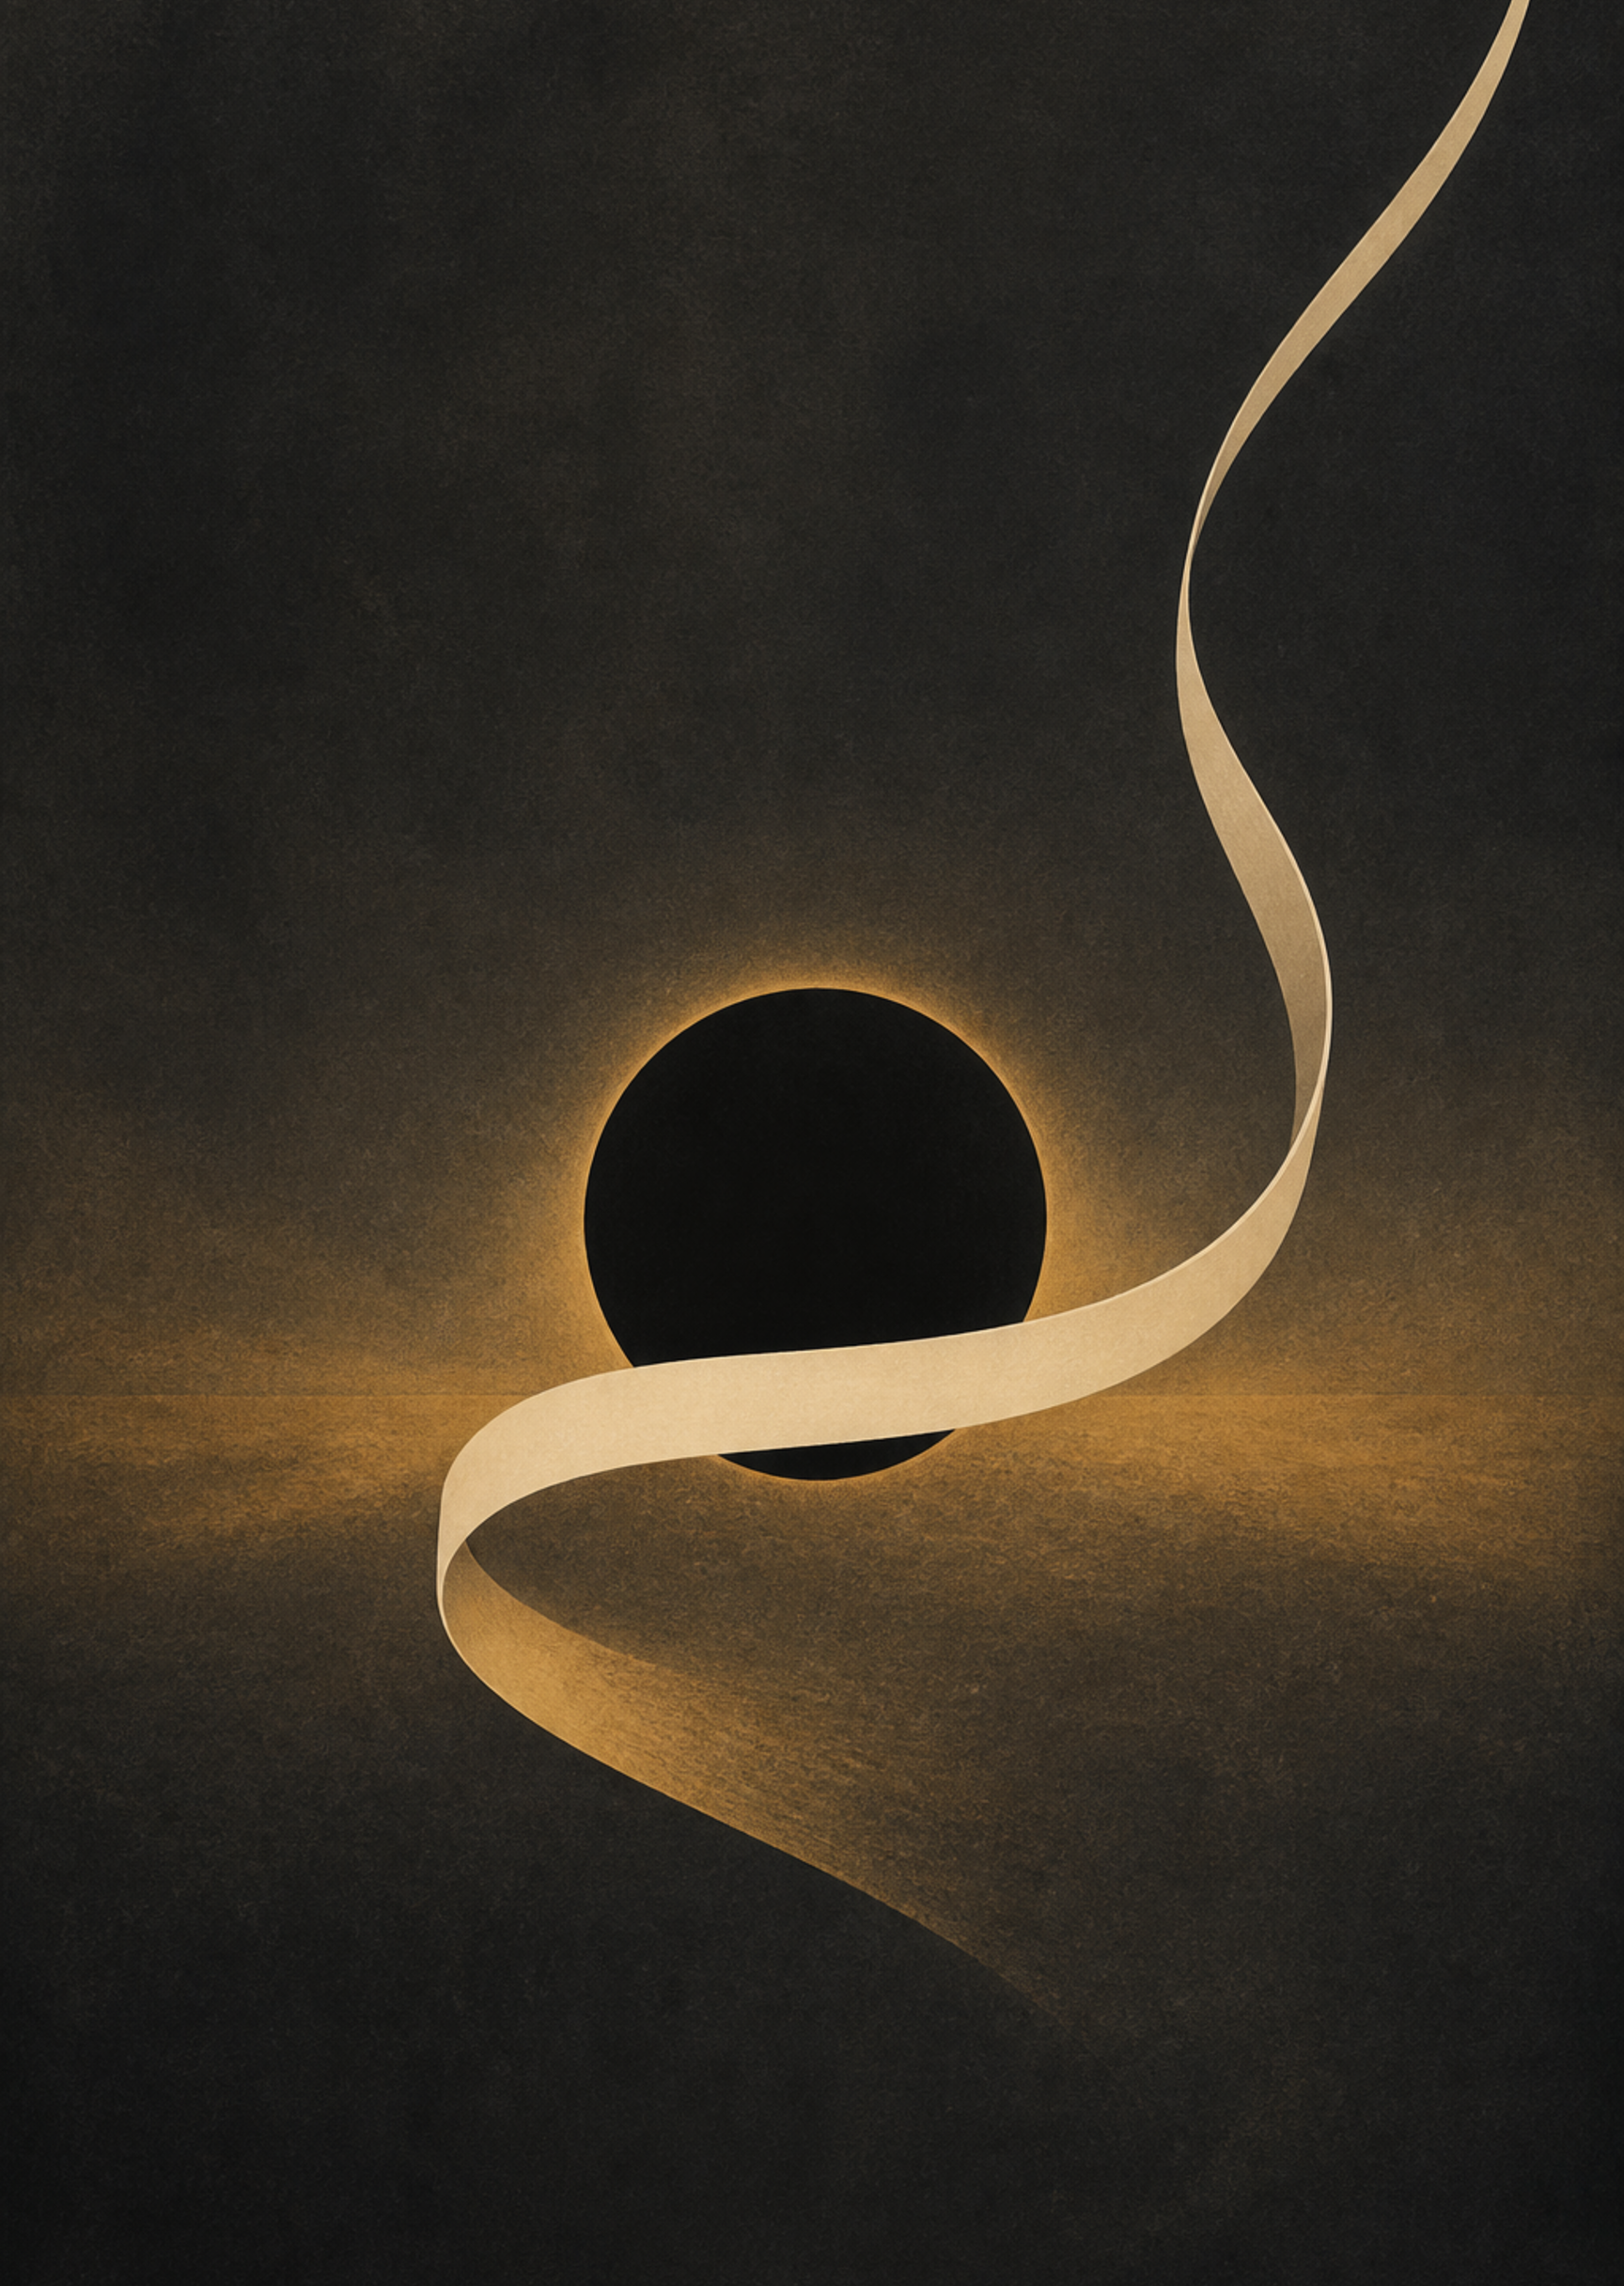
\includegraphics[height=\paperheight,keepaspectratio]{../../../generated_course_notes/supplementary/cosmology_and_black_holes/2011_winter_topics_in_string_theory/assets/cover-art.png}%
  };
  \node[
    anchor=north west,
    align=left,
    text width=0.78\paperwidth,
    fill=white,
    fill opacity=0.9,
    rounded corners=8pt,
    inner xsep=10pt,
    inner ysep=8pt
  ] at ([xshift=0.08\paperwidth,yshift=-0.06\paperheight]current page.north west) {%
    {\fontsize{30}{33}\selectfont\bfseries\color{black!88} 弦理論の諸問題\\[0.85em]}
    {\large\color{black!72} 日本語版 / 2011 winter topics in string theory}
  };
  \node[
    anchor=south west,
    align=left,
    text width=0.68\paperwidth,
    fill=white,
    fill opacity=0.82,
    text opacity=1,
    rounded corners=6pt,
    inner sep=12pt
  ] at ([xshift=0.08\paperwidth,yshift=0.08\paperheight]current page.south west) {%
    {\normalsize\color{black!78} 原講義：Leonard Susskind\\[0.35em]}
    {\small\color{black!72} 講義補助版：\href{https://lazying.art}{LazyingArt LLC} / \href{https://github.com/lachlanchen/Video2Book}{Video2Book}}
  };
\end{tikzpicture}
\mbox{}
\end{titlepage}
\hypersetup{pageanchor=true}

\clearpage
\chapter*{本ノートについて}
本独立編集のコンパニオンノートは、Leonard Susskind による講義に基づくものである。これらは機械文字起こし、字幕、および選択された黒板画像から再構成され、その後、利用可能な原資料と照合して確認された。これは Susskind 教授による原著原稿ではなく、同教授による査読や承認を受けたものでもない。

本版は \href{https://lazying.art}{LazyingArt LLC} がオープンソースの \href{https://github.com/lachlanchen/Video2Book}{Video2Book} ツールキットを用いて作成した。機械文字起こしは別途入手可能であり、認識誤りを含む可能性がある。編集上の明確化および自明でない再構成は脚注で示されている。
\clearpage
\tableofcontents
\mainmatter
\chapter{講義 1：弦理論の諸問題}

\lectureoverview{還元主義への挑戦は、\(1+1\)次元におけるボソン化、電気--磁気双対性、Dブレーン、強結合転移、創発的幾何、そして弦真空の組合せ的ランドスケープを通じて鋭くなる。同じ物理系が根本的に異なる素朴な記述を持ちうる。どちらの記述が単純に見えるかは、結合定数と幾何に依存する。}

\section{還元主義、複雑性、そして単純さの問題}

サスキンドは、意図的に親しみやすい哲学的スローガンから始める。大きなものは小さなものからできており、小さなものはさらに小さなものからできている、というものである。次に彼は同じ考えのより野心的な版、基礎物理学にとって本当に重要な版を付け加える。より深い層へと降りていくにつれて、対象はより小さくなるだけでなく、より単純にもなるはずだ、というものである。彼の比喩は、家はレンガからできており、家をレンガと間違える人はいない、というものである。レンガはより小さいが、より単純でもある。

この講義の最初の一手は、その期待を素粒子物理学の実際の状況と突き合わせることである。もし還元主義がその強い意味で増大する単純さをもたらしているのなら、現在の素粒子物理学は簡素に近いはずだと期待されるかもしれない。そうではなく、サスキンドは、量子重力が入る前でさえ、帳簿付けはすでに messy に見えると強調する。講義ではこれらは粗い数え上げであるが、その粗さ自体が論点の一部である：
\begin{equation}
\begin{aligned}
N_{\mathrm{species}}&\sim 75,\\
N_{\mathrm{independent}}&\sim 10\text{--}20,\\
N_{\mathrm{parameters}}&\sim 20.
\end{aligned}
\end{equation}
話はこれで終わらない。標準模型は重力を含まず、暗黒物質を説明せず、インフレーションに必要な余分な構造を与えず、深刻な微調整問題を抱えている。通常の修復機構を加えると、数え上げは増えるだけである。超対称性が講義の例である。講義の時点で、多くの物理学者は大型ハドロン衝突型加速器が超対称パートナーを露わにすることを望んでいた。サスキンドは、対応する拡張は帳簿付けを直ちに単純化するどころか、百を超える追加パラメータを導入することになると強調する。彼の図式的なメッセージは
\begin{equation}
N_{\mathrm{parameters}}^{\mathrm{extended}} \sim 200.
\end{equation}
これらの数は意図的に粗く、歴史的なものである。それらは、より深い記述が、その粒子の目録と測定された定数のレベルで必ずしもより単純に見える必要はない、という議論に資する。

この定量的な不満は、まだサスキンドの主テーゼではない。それは前奏曲である。より深い主張、そして講義の残りを駆動する主張は、現代の量子場理論と弦理論が、レンガと家の間の一意で結合定数に依存しない区別を明らかに支持しているわけではない、というものである。次の例は、``素粒子''の意味そのものが、どの変数が効率的であるかに依存しうることを示すために選ばれている。

\section{ボソン化：固定された基礎性の最初の崩壊}

サスキンドの最初の理論的例は、\(1+1\)次元量子場理論、すなわち空間一次元、時間一次元から来る。彼はすぐに、その等価性を詳細に導出するつもりはないと宣言する。要点は形式的な証明ではなく、概念的教訓である。

フェルミオンの場の理論から始める。フェルミオン場は\(\psi\)で表される。近接する二つのフェルミオンはボソン的複合体を形成しうる。対応するボソン場は\(\phi\)で表される。一見すると階層は単純に見える。\(\psi\)が基本的であり、\(\phi\)は複合または有効変数である。講義では、ボソンはまさにこのように、フェルミオンの束縛対を生成する場として導入される。

しかし発見されたのは、同じ理論が反対の出発点から書き直せるということである。ボソン場\(\phi\)から始めてもよい。するとフェルミオンはもはや点状の構成要素として現れない。代わりに、ボソン場のキンク、すなわち\(\phi\)が二つの漸近値の間を滑らかに補間する拡張的配置として現れる。講義の最小限の数学的内容はこの漸近構造である：
\begin{equation}
\phi(x\to -\infty)=\phi_-,
\qquad
\phi(x\to +\infty)=\phi_+.
\end{equation}
便利な図式的代表は
\begin{equation}
\phi(x)\approx \frac{\phi_++\phi_-}{2}
+
\frac{\phi_+-\phi_-}{2}\tanh\!\left(\frac{x}{\ell}\right),
\end{equation}
ここで\(\ell\)は遷移領域の幅である。

\editorialnote{双曲線正接のプロファイルは、講義で描かれたキンクの標準的な滑らかな代表であり、そこで導出された式ではない。正確なボソン化の辞書は模型に依存する。概念的な要点は、フェルミオン的励起とボソン場のトポロジカルソリトンの間の交換である。}

講義で用いられたベルトの類推は、保持する価値があるほど精密である。ねじれのない平らなベルトは、キンクを持たない配位である。一端を\(2\pi\)だけ回転させると、ベルトは遠方で同じ局所的向きに戻るが、その間では広がったねじれ領域を通らなければならない。そのねじれ領域がキンクである。ボソン的記述では、フェルミオンはまさにそのような広がった対象によって表される。

結合を導入すると、この点はより鮮明になる。Susskindはこの例でそれを\(G\)と呼んでいる。主張は、二つの記述が漠然と関係しているということではなく、二つの記述の効率がパラメータ領域に依存するということである：
\begin{align}
G \ll 1
&\Rightarrow
\ell\text{ small, tight kink; }\psi\text{ efficient},\\
G \gg 1
&\Rightarrow
\ell\text{ large, broad kink; }\phi\text{ efficient}.
\end{align}
\(G\)が小さいとき、キンクは引き締まっており、フェルミオンは単純な対象のように見える。\(G\)が増大すると、キンクは広がり、フェルミオンは点状ではなくなる。そのときボソン的変数のほうがより経済的になる。

\paragraph{概略的な更新規則。}
\begin{enumerate}
\item \(\psi\)で記述されるフェルミオン的理論から始める。
\item \(\phi\)で記述されるボソン的複合体を同定する。
\item 同じ理論を完全に\(\phi\)の言葉で書き直す。
\item ボソン的記述では、フェルミオンは幅\(\ell\)のキンクとして再現する。
\item \(G\ll 1\)では、\(\ell\)は小さく、フェルミオン的記述が最も単純である。
\item より大きな\(G\)では、\(\ell\)が成長し、ボソン的記述が最も単純になる。
\end{enumerate}

これは、固定された``家とレンガ''という描像に対する最初の明示的な反例である。講義の落ちは、複合的な対象が存在するというだけではなく、何が要素的変数とみなされるかが結合によって変わりうるということである。

\section{電荷、磁気単極子、および弱結合対強結合}

次にSusskindは、同様の話がより身近な素粒子物理学にも現れるかと問う。例は電荷対磁気単極子である。電子のような通常の荷電粒子は、この言葉では電気単極子である：電場の局在した源である。磁気単極子は棒磁石の類推によって導入される。もし棒磁石の端を、目に見えない連結棒なしに何とか単離できたなら、場の線は電荷のそれとまったく同じに見えるだろうが、電気的ではなく磁気的である。

関連する制御パラメータは微細構造定数\(\alpha\)である。講義でSusskindはそれを電荷の二乗として発見法的に扱う：
\begin{equation}
\alpha \sim e^2.
\end{equation}
また彼は粗い操作的解釈も与えている：それは電子がどれほど容易に放射するかを測るものであり、彼はその強さを、加速された電子は関連する意味でおよそ``\(1/100\)''個の光子を放射すると述べることで要約している。講義自身の粗い数値的言葉では、
\begin{equation}
\alpha \approx 10^{-2}.
\end{equation}
これは精密な規約として意図されたものではなく、電荷が弱いことを符号化する教育的な方法である。

\editorialnote{弱--強の関係には、ディラック量子化という精密な祖先がある。よく用いられる一つの規約では、電気的電荷と磁気的電荷は\(e g_m=2\pi n\)を満たす。したがって、弱い電気的結合は強い磁気的結合に対応するが、正確な数値因子や保護された質量関係は理論に依存する。}

\(\alpha\ll 1\)のとき、電子が単純な対象である。その電場は弱く、その真空偏極の雲は希薄で、ほとんど点状に見える。そのとき磁気単極子は反対である：その場は巨大で、その周囲は激しく歪み、それは広く、複雑で、重い。Susskindはこの状況をまさにこの弱--強の様式で要約している：
\begin{equation}
\begin{aligned}
\alpha \ll 1
&\Rightarrow \text{simple electron;}\\
&\phantom{\Rightarrow{}}\text{heavy, extended monopole},\\
\alpha \gg 1
&\Rightarrow \text{simple monopole;}\\
&\phantom{\Rightarrow{}}\text{heavy, structured electron}.
\end{aligned}
\end{equation}
講義は単極子の質量公式を導出しない。その必要もない。要点は定性的である。\(\alpha\)が増大すると、電子の場は強まりその構造は成長し、一方で単極子は縮み軽くなる。1をはるかに超えると、有用な記述は交換される：単極子が単純で、電子が複雑になる。

これが、先のボソン化からの教訓の場の理論版である。基本的なものと複合的なものの区別は絶対的ではない。それは結合に依存する。

\begin{classroomqa}
\audiencequestion{もし還元主義が信頼できる指針でないなら、なぜ物理学者は、系を任意に小さな断片に分割するように見える微積分に依拠するのか。\lecturetimestamp{00:21:21}}
\lecturerresponse{微積分は滑らかな変化を主張するが、理論の基本的対象を同定するものではない。量子場はあらゆる距離スケールで揺らぎ、何が要素的かを一度きりで決められる最終的な滑らかな層ではなく、終わりのない階層を生み出す。}
\end{classroomqa}

このやり取りは、階層性がフラクタルに似ているという示唆へと続く。サスキンドはその類推を受け入れ、さらにそれを鋭くする。量子場はあらゆるスケールで揺らぐため、古典的な意味で決して滑らかではない。この過剰な変動こそが量子場理論を数学的に難しくしている一因であり、通常の微積分は、素朴に滑らかな微視的場に対してではなく、繰り込み済みの量に対して用いなければならない。

\section{弦、Dブレーン、そして弱--強双対性の回帰}

講義における次の移行は、意図的に素朴である。もし弦理論が基本的な構成要素の理論であるはずなら、答えはきっと単純に違いない。構成要素とは弦である。サスキンドはその期待を率直に述べ、そして講義の次の部分をその解体に費やす。

\subsection{なぜ弦がすべてではないのか}

最初の厄介な点は、避けがたく存在するDブレーンである。D\(p\)ブレーンは、弦が端を置ける\(p\)次元の物体である。文字\(D\)はディリクレ境界条件に由来するが、その名はその役割ほど重要ではない。これらの物体は理論の一部であり、捨て去ることはできない。それらは任意の飾りではない。

最も単純な例は次のとおりである。
\begin{itemize}
\item 点状であるD0ブレーン、
\item 弦状であるD1ブレーン、すなわちD弦、
\item 通常の基本弦であるF弦。
\end{itemize}
D0ブレーンは、任意の数のF弦が端を置ける重い点状の場所である。D1ブレーンは重いケーブル状の物体であり、F弦よりもはるかに太く、単位長さあたりの質量も大きいが、同様にF弦が端を置ける場所である。弱結合では、講義はこれらの物体を等しく基本的な選択肢として提示しない。Dブレーンは、重く、構造を持ち、複合的に見える物体として導入されるが、それでも理論が我々に強いるものである。

\editorialnote{講義のこの部分で用いられる奇数ブレーン理論は、タイプIIB弦理論である。その安定なDブレーンは、D1ブレーンやD3ブレーンを含む奇数空間次元を持つ。サスキンドがこれらの名称を後回しにするのは、分類ではなく双対性のパターンが当面の主題だからである。}

\paragraph{記法。}
サスキンドは講義の異なる部分で\(G\)と\(g\)をやや緩く用いている。ここでは\(G\)はボソン化の例のために取っておかれ、一方\(g\)は弦結合定数を表す。

弦結合定数\(g\)は、公理的にではなく操作的に定義される。それは、揺らぐ弦が分裂して娘弦を形成する確率を測るパラメータである。だからこそサスキンドは、それをQEDにおける\(\alpha\)の役割に直接比較する。講義はまた、張力を単位長さあたりのエネルギーと同定するために一息つく。
\begin{equation}
T=\frac{E}{L}=\frac{M}{L}.
\end{equation}

F弦とD弦について、標準的な張力の公式は弱--強の比較を明示的にする。
\begin{equation}
T_{\mathrm{F1}}=\frac{1}{2\pi\alpha'},
\qquad
T_{\mathrm{D1}}=\frac{1}{2\pi\alpha' g_s},
\qquad
\frac{T_{\mathrm{D1}}}{T_{\mathrm{F1}}}=\frac{1}{g_s}.
\end{equation}
\editorialnote{これらの張力の公式は、講義の定性的なケーブルと糸の比較の背後にある従来の規格化を与える。それらは編集上の追加であり、講義は結合定数によるスケーリングのみを用いている。}

\subsection{F弦とD弦}

弱--強の物語は、ここで弦の言葉で繰り返される。小さな結合定数では、F弦は軽く、細く、基本物体という元々の直観的イメージに近い。D弦は太く、重く、F弦の構造に満ちている。結合定数が大きくなるにつれて、F弦はより容易に分裂し、その周りに娘弦の雲が増殖し、F弦はより重く複雑になる。同時に、D弦は今や重くなったF弦を放出することがますます難しくなるため、その周囲の構造は薄くなり、D弦はより軽く、より線状になる。したがって講義の弱--強の対応は
\begin{align}
g \ll 1
&\Rightarrow
\begin{gathered}
\text{F-string light and thin;}\\
\text{D-string heavy and structured},
\end{gathered}\\
g \sim 1
&\Rightarrow
\text{F-string and D-string comparable},\\
g \gg 1
&\Rightarrow
\begin{gathered}
\text{D-string light and thin;}\\
\text{F-string heavy and structured}.
\end{gathered}
\end{align}
サスキンドは、\(g\sim 1\)付近で二つの記述が鋭く区別されなくなる、と述べる。その点を超えると、それらは事実上役割を交換する。これは電子--磁気単極子の交換の弦理論版であり、その受け入れられた名称はS双対性である。

同じ交換は、弦が閉じてループになった後にも追跡できる。弱結合では、小さなF弦ループは軽い粒子様励起であり、対応するD弦ループは重く複雑である。強結合ではそれらの役割が逆転する。D弦ループが軽い記述となり、その結果生じる軽い閉弦励起の中には重力子が含まれる。講義はこの例を用いて、なじみ深い粒子の同一性さえも、双対性のどちら側を用いるかに依存しうると主張する。

講義はこの点をさらに一歩押し進める。理想化された理論では、結合定数は単に手で調整する数ではない。それは場のように振る舞う。模式的には、
\begin{equation}
g = g(x).
\end{equation}
したがって、空間の異なる領域は異なる双対記述を好むことがあり得る。ある領域ではF弦が軽い変数であり、別の領域ではD弦がそうである。その中間では、何も特に単純ではない。だからこそSusskindにとって、弦理論は単純な還元主義的描像を回復するものではない。それは曖昧さを先鋭化するのである。

\editorialnote{摂動弦理論では、局所的な結合定数はディラトン\(g_s(x)=e^{\Phi(x)}\)によって定まる。したがって\(g=g(x)\)と書くことは単なる類推ではない。ただし、現実的なコンパクト化は一般にそのような変動を制約するポテンシャルを生じる。}

\begin{classroomqa}
\audiencequestion{結合定数が十分に変動して、別の領域でD弦がF弦より軽くなるなら、その変化は観測可能なスペクトルに影響するだろうか。\lecturetimestamp{00:34:15}}
\lecturerresponse{はい。それが、議論されている完全に対称で数学的に制御された模型を、我々の世界と直接同一視できない理由の一つである。その教訓は、整合的な量子理論が何をなし得るかに関するものであり、自然の文字通りのスペクトルに関するものではない。}
\end{classroomqa}

\begin{classroomqa}
\audiencequestion{D2ブレーンにも類似の双対記述があるだろうか。\lecturetimestamp{00:34:39}}
\lecturerresponse{はい、しかしそれは別のD弦的な交換ではない。偶数ブレーンの場合は膜解釈と追加の空間次元へと導く。それが次の構成である。}
\end{classroomqa}

\begin{classroomqa}
\audiencequestion{弦が分裂する確率が大きいことが、内部複雑性の増大を説明するのだろうか。\lecturetimestamp{00:34:53}}
\lecturerresponse{はい。機構を具体的にするためにQEDに戻ろう。電子は光子を放出し、光子は荷電対へと揺らぎ、それらの荷電線は再び放射する。結合定数を大きくすると、その階層はより希薄でなくなる。}
\end{classroomqa}

\subsection{問いに駆動された量子電磁力学への回帰}

次に学生が、分裂確率が大きいことは単により複雑な構造が``上流に''あるということを意味するだけなのかと尋ねる。Susskindは量子電磁力学に戻り、再び電子の世界線を描くことで答える。この回帰は重要である。それは、弦の話が孤立した珍奇さではなく、同じ弱--強のパターンのもう一つの実例であることを示すからである。

\begin{figure}[htbp]
\centering
\begin{tikzpicture}[scale=1.0]
\draw[->] (-1.2,0) -- (3.7,0) node[right] {space};
\draw[->] (0,-0.2) -- (0,4.3) node[above] {time};

\draw[line width=0.9pt] (0,0.2) -- (0,4.0);
\node[left] at (0,3.55) {\(e^{-}\)};

\draw[line width=0.8pt] (0,1.0) -- (0.18,1.08) -- (0.36,0.92) -- (0.54,1.10) -- (0.72,0.94) -- (0.90,1.12) -- (1.08,0.96) -- (1.26,1.14);
\draw[line width=0.8pt] (0,2.35) -- (-0.18,2.43) -- (-0.36,2.27) -- (-0.54,2.45) -- (-0.72,2.29) -- (-0.90,2.47);

\draw[line width=0.8pt] (1.26,1.14) -- (1.48,1.42);
\draw[line width=0.8pt] (1.26,1.14) -- (1.04,1.42);
\draw[line width=0.8pt] (1.48,1.42) -- (1.58,2.10);
\draw[line width=0.8pt] (1.04,1.42) -- (0.94,2.10);
\draw[line width=0.8pt] (0.94,2.10) -- (1.58,2.10);

\draw[line width=0.7pt] (1.58,1.78) -- (1.72,1.84) -- (1.86,1.72) -- (2.00,1.86);
\draw[line width=0.7pt] (0.94,1.78) -- (0.80,1.84) -- (0.66,1.72) -- (0.52,1.86);

\node at (2.35,1.95) {\(\gamma\)};
\node at (-1.15,2.75) {\(\gamma\)};
\end{tikzpicture}
\caption{講義で用いられた模式的なQED階層：点状電子が光子を放出し、光子が対を生成し、娘の荷電線が再び放射し、次第に短いスケールで構造を生じる。}
\end{figure}

講義の要点は、点状電子でさえ過程の階層を伴うということである：
\begin{enumerate}
\item 電子は光子を放出し吸収する、
\item 光子は電子--陽電子対を生成し得る、
\item 娘の荷電線自身が光子を放出し得る、
\item 階層はより小さなスケールへと続く。
\end{enumerate}
弱結合ではこの雲は希薄であり、したがって電子は実験室ではほとんど点状に見える。より強い結合ではそれは増殖し、電子は構造を持つ対象となる。弦の話は、このことの直接の類似として提示される。

同じ後半の議論は、Susskindのヒューリスティックなエネルギー計算の動機にもなっている。彼は、関係するエネルギーが単に自由粒子の寄与の和ではないと主張する。相互作用エネルギーも含めなければならない：
\begin{equation}
E_{\mathrm{tot}} = E_e + E_\gamma + E_{\mathrm{int}}.
\end{equation}
ここで\(E_{\mathrm{int}}\)が決定的な項である。これによって、着衣電子の質量が、その周囲の場と仮想構造に伴うエネルギーを含むことができる。講義はこれを形式的な繰り込み自己エネルギーの導出にはしない。要点はヒューリスティックだが本質的である：対象の質量は、その周りの複雑な雲を支えるのに必要な相互作用エネルギーをすでに含んでいる。

\begin{classroomqa}
\audiencequestion{電子が実対を生成するのに十分な自由エネルギーを含まないなら、仮想光子と電子--陽電子対のエネルギーはどこから来るのか。\lecturetimestamp{00:37:01}}
\lecturerresponse{裸の電子から始めて後からそのクーロン場を付けるということは決してない。観測される電子は着衣状態であり、その質量はすでに場と相互作用のエネルギーを含んでいる。QEDでは全エネルギーは自由電子のエネルギーと自由光子のエネルギーのみの和ではない。相互作用項が不可欠である。中間の対を仮想と呼ぶのは有用だが、エネルギーの計算は完全な相互作用状態に属する。}
\end{classroomqa}

\begin{classroomqa}
\audiencequestion{高エネルギーの探針がこの構造を明らかにするとき、探針はすでに存在していた何かを発見したのではなく、それを創り出したのだろうか？\lecturetimestamp{00:38:59}}
\lecturerresponse{その解釈上の区別は議論の余地がある。操作上は、十分に高エネルギーの散乱は計算可能で非自明な終状態を持つ。弱結合ではほとんどの事象は依然として単純に見えるが、およそ\(\alpha\)程度の割合で追加の放射や対が現れる。}
\end{classroomqa}

\begin{classroomqa}
\audiencequestion{D1ブレーンがF弦よりも重いと言われるとき、その張力もまた大きいのか？\lecturetimestamp{00:39:37}}
\lecturerresponse{はい。拡がった弦にとって、ここでの``質量''とは単位長さあたりのエネルギーを意味し、それはまさに張力である。}
\end{classroomqa}

\begin{figure}[htbp]
\centering
\includegraphics[width=0.72\textwidth]{lecture_01_figure_02.png}
\lectureframe{00:38:22.500}

\vspace{1em}

\begin{tikzpicture}[scale=0.95]
\draw (-5.3,-2.4) rectangle (-1.0,2.1);
\draw (0.3,-2.4) rectangle (4.6,2.1);

\node at (-3.15,2.55) {$\alpha \ll 1$};
\node at (2.45,2.55) {$\alpha \gg 1$};

\draw[line width=0.9pt] (-3.15,-0.15) circle (0.22);
\draw[->,line width=0.8pt] (-3.15,0.07) -- (-3.15,1.35);
\draw[->,line width=0.8pt] (-2.98,-0.01) -- (-1.95,1.00);
\draw[->,line width=0.8pt] (-3.32,-0.01) -- (-4.35,1.00);
\draw[->,line width=0.8pt] (-2.95,-0.23) -- (-1.80,-0.95);
\draw[->,line width=0.8pt] (-3.35,-0.23) -- (-4.50,-0.95);

\draw[line width=1.0pt] (2.15,-1.8) .. controls (1.95,-0.6) and (1.95,0.8) .. (2.15,1.55);
\draw[line width=1.0pt] (2.75,-1.8) .. controls (2.95,-0.6) and (2.95,0.8) .. (2.75,1.55);
\draw[line width=0.8pt] (2.15,-0.85) -- (2.75,-0.85);
\draw[line width=0.8pt] (2.45,1.55) -- (2.45,1.95);
\end{tikzpicture}
\caption{相互作用エネルギーの議論における弱--強QEDの比較。この図はSusskindの周辺で見える二つの領域、すなわち希薄な弱結合の雲と増殖する強結合の雲を分離して示している。}
\end{figure}

弱--強の比較は以前に導入されたにもかかわらず、この図がここに属する理由は、講義においてSusskindが相互作用エネルギーと増殖する構造を議論しながら、この後の質問に駆動された時点で対比を描き直すからである。

\section{偶数ブレーン理論と創発する余剰次元}

ここまで、講義は交換について強い物語を語ってきた。フェルミオン対ボソン、電子対モノポール、F弦対D弦である。次の段階はより驚くべきものである。Susskindは弦理論の別のバージョンへと切り替える。奇数次元のDブレーンではなく、偶数次元のDブレーンを持つものである。この区別が重要であるのは、この理論にはF弦と交換すべきD弦が存在しないからである。D0ブレーン、D2ブレーン、D4ブレーンなどがある。

したがって強結合極限は、単にある弦を別の弦としてラベル付けし直すことではありえない。講義によれば、もっと奇妙なことが起こる。余分な空間次元が顕在化するのである。Susskindは意図的にこれを最も劇的な形でまず述べる--- ``新しい次元が実体化する'' ---、そして直ちにより慎重な表現に翻訳する。非常に小さなコンパクトな方向が膨張し、もはや無視できなくなるのである。

帳簿付けは論点の一部であるため、彼はそこで間を置く。
\begin{equation}
\begin{aligned}
10\text{-dimensional string theory} &= 9\text{ space}+1\text{ time},\\
11\text{-dimensional theory} &= 10\text{ space}+1\text{ time}.
\end{aligned}
\end{equation}
講義の主張は、偶数ブレーン理論の強結合極限が事実上11次元であるというものである。

\editorialnote{偶数ブレーン理論はType IIA弦理論であり、その強結合完備化はM理論である。標準的な単位では、創発する円の半径と11次元プランク長は\(R_{11}=g_s\ell_s\)および\(\ell_{11}=g_s^{1/3}\ell_s\)のようにスケールする。これらの名称と公式は、講義の幾何学的な説明の背後にある現代的な辞書を明示している。}

\subsection{ピーナッツバターサンドイッチ}

コンパクトな方向を思い描くために、Susskindは``ピーナッツバターサンドイッチ''模型を用いる。無限に薄い二枚のパンがあり、その間に実空間が存在する。特別な規則は、一方の側から出ると他方の側に戻るというものである。講義が形式的ではなく絵的に説明する従来の記法では、次のように書ける。
\begin{equation}
y \sim y + 2\pi R.
\end{equation}
もし\(R\)が非常に小さければ、サンドイッチの中に住む観測者は自分の世界を事実上低次元として記述する。そのとき鍵となる強結合の更新は
\begin{equation}
g\uparrow
\qquad \Longrightarrow \qquad
R_{\mathrm{compact}}\uparrow.
\end{equation}
である。これが、Susskindが空間の新しい次元が現れると言うときに意味することである。すなわち、空間が無から創られるのではなく、以前は小さかったコンパクトな方向が膨張し、有効理論において可視的になるのである。

\begin{figure}[htbp]
\centering
\resizebox{\linewidth}{!}{%
\begin{tikzpicture}[scale=0.95]
\draw[line width=0.9pt] (-5,1.7) -- (5,1.7);
\draw[line width=0.9pt] (-5,-1.7) -- (5,-1.7);

\node[left] at (-5,1.7) {ceiling};
\node[left] at (-5,-1.7) {floor};

\draw[->,line width=0.8pt] (5.2,1.45) -- (5.2,-1.45);
\draw[->,line width=0.8pt] (5.5,-1.45) -- (5.5,1.45);
\node[right] at (5.55,0) {periodic};

\draw[line width=1.0pt] (-2.6,0.45) -- (2.2,0.45);
\draw[line width=1.0pt] (-2.6,-0.05) -- (2.2,-0.05);
\draw[line width=1.0pt] (-2.6,0.45) -- (-2.6,-0.05);
\draw[line width=1.0pt] (2.2,0.45) -- (2.2,-0.05);
\node at (-0.2,0.9) {floating D2-brane};

\draw[line width=1.0pt] (3.15,-1.7) -- (3.8,-1.7);
\draw[line width=1.0pt] (3.15,1.7) -- (3.8,1.7);
\draw[line width=1.0pt] (3.15,-1.7) -- (3.15,1.7);
\draw[line width=1.0pt] (3.8,-1.7) -- (3.8,1.7);
\node[right] at (3.95,0) {D2 ribbon};

\fill (-3.8,0) circle (0.07);
\node[below] at (-3.8,-0.05) {D0};
\end{tikzpicture}
}%
\caption{サンドイッチコンパクト化。上下の境界は周期的に同一視され、一つのD2ブレーンは絨毯のようにそれらの間を浮かび、別のものは床から天井まで伸び、コンパクトな方向が小さいときには弦のように見える。}
\end{figure}

\subsection{D0ブレーンとD2ブレーンはどうなるのか？}

講義は今、D0ブレーンと弦がどうなるかを問う。答えは非対称である。\(g\)が大きくなるにつれて、D0ブレーンはますます軽くなり、高次元の解釈では新たに顕在化した方向に運動量を持つ粒子の塔に加わる。こうして、弱結合の描像における重く複雑な物体が、強結合の描像における通常の軽い励起となる。

質量関係は次の同一視を示している：
\begin{equation}
M_{D0}(n)=\frac{n}{g_s\ell_s}
=\frac{n}{R_{11}}
=M_{\mathrm{KK}}(n).
\end{equation}
\editorialnote{SusskindはD0ブレーンを11次元理論の``重力子''と呼んでいる。より正確には、それらの束縛状態が11次元超重力多重項のKaluza--Klein運動量モードであり、その質量ゼロのセクターには重力子が含まれる。この区別は、講義における物理的な同一視を保ちつつ、文字通りの一粒子の過大評価を避けている。}

D2ブレーンは弦の運命を説明する。講義で強調される配置は二つある：
\begin{enumerate}
\item ピーナッツバターの中のカーペットのように床と天井の間に浮かぶD2ブレーン；
\item リボンのように床から天井へ張られ、可視方向に沿って伸びたD2ブレーン。
\end{enumerate}
サンドイッチが薄いとき、リボンは実効的に一次元に見える。低エネルギー観測者が弦と呼ぶのはこの物体である。コンパクト方向が開くにつれて、同じ物体は紛れもなく膜的なものになる。垂直方向により多くの物質を含むようになるため、重くなり、弦らしくなくなる。

\paragraph{移行の論理。}
\begin{enumerate}
\item 非常に薄いコンパクト方向から始めると、床から天井へのリボンは実効的に弦のように振る舞う。
\item \(g\)を増やすと、コンパクト方向が膨張する。
\item D0ブレーンは軽くなり、高次元理論におけるKaluza--Klein運動量状態として再解釈される。
\item 弦のようなD2リボンは目に見えて伸びた膜となり、重くなる。
\end{enumerate}
これが、双対性から創発的幾何学への講義の蝶番である。強結合は単にある物体を別の物体に交換するのではなく、どちらの幾何学が効率的であるかを変える。

Susskindはこれがどれほど奇妙に聞こえるかについてしばし留まる。提案された同一視の網は困難な数学的整合性関係を必要とし、そのうちのいくつかは最初に物理学者たちに予想として現れ、後に数学者たちによって確立された。彼の主張は、あらゆる現実的な弦の真空が理解されているということではなく、双対性の網そのものが異常に厳しい検証を生き延びてきたということである。

この理想化された設定で結合が場所ごとに変化するならば、効率的な幾何学もそれに伴って変化しうる。ある領域は軽い弦と重いD0ブレーンを伴うほとんど10次元に見えるかもしれず、別の領域は重い巻き付いた膜と軽いKaluza--Kleinモードを伴う11次元記述へと開くかもしれない。言語の局所的な変化は同じ双対性の網の一部である。

記録はこれらの関係の名称を一時的に``不等式''と表記している。文脈上、意図された語は\emph{双対性}である：パラメータ空間の両端の間の関係である。この訂正が重要であるのは、講義の結論がまさに、基本的構成要素の一意なリストは知られていないというものであるからだ。弦、ブレーン、粒子、高次元幾何学は互いに変換しうる；網のどの成員も絶対的に基本的でないか、あるいは何らかのより深い組織化が未知のまま残っているかのいずれかである。

\section{D3ブレーン、巻き付いた膜、そして双対性の幾何学的描像}

休憩の後、Susskindはこの主題を相互に結びついた理論とアイデアの``巨大な網''であると明示的に述べる。次の例は新たな孤立した効果ではなく、以前のものを結び合わせる橋である。

\subsection{D3ブレーンの世界体積}

最初の橋はD3ブレーンを用いる。D3ブレーンは三つの空間次元を持ち、それに閉じ込められた観測者はそれを通常の空間と容易に誤認しうる。ブレーンは曲がり揺らぐことができ、一方それに端点を持つ弦は結合し、分裂し、散乱しうる。ブレーンに沿った方向のみを見る観測者にとって、各端点は粒子のように見え、端点間の相互作用は通常の量子場理論のように見える。

\begin{figure}[htbp]
\centering
\resizebox{\linewidth}{!}{%
\begin{tikzpicture}[scale=1.0]
\draw[fill=gray!15] (-4,-0.35) rectangle (4,0.35);
\node at (0,-0.75) {D3-brane};

\draw[line width=0.9pt] (-1.5,2.1) -- (-1.5,0.35);
\fill (-1.5,0.35) circle (0.07);
\node[left] at (-1.72,1.25) {F-string};
\node[below left] at (-1.5,0.32) {electric charge};

\draw[line width=1.5pt] (1.7,2.1) -- (1.7,0.35);
\fill (1.7,0.35) circle (0.09);
\node[right] at (1.95,1.25) {D-string};
\node[below right] at (1.7,0.32) {magnetic monopole};
\end{tikzpicture}
}%
\caption{D3ブレーンの世界体積解釈。F弦の端点は電荷として現れ、D弦の端点は磁気単極子として現れる。}
\end{figure}

これは講義の中でも最も満足のいく同一視の一つである。D3ブレーンに端点を持つF弦は、世界体積の観測者には電荷として現れる。同じブレーンに端点を持つD弦は磁気単極子として現れる。言い換えれば、F弦とD弦の間の双対性は、D3ブレーンの世界体積上で、通常の場の理論の電磁双対性--となる。以前は類推であったものが、今や明示的な辞書となっている。

\editorialnote{D3ブレーンを重ねたものの低エネルギー世界体積上の記述は、四次元\(\mathcal N=4\)超対称Yang--Mills理論である。その電気--磁気双対性は、IIB型S双対性の場の理論における実現である。単一のブレーンは、講義で図的に用いられた可換極限を与える。}

\subsection{二つのコンパクト方向と非対称な巻き付き}

次にSusskindは高次元の幾何学に戻り、一つではなく二つの小さな方向をコンパクト化する。黒板に11次元を描くことはできないので、彼はスケッチで用いていない七つの大きな方向を一つの見える水平方向に押し込み、次に二つのコンパクトな方向を明示的に描く。彼はコンパクト化を非対称に描くことにこだわる。なぜなら、有効な弦が異なる張力をもつためには、一方のコンパクト方向が他方より短くなければならないからである。

\begin{figure}[htbp]
\centering
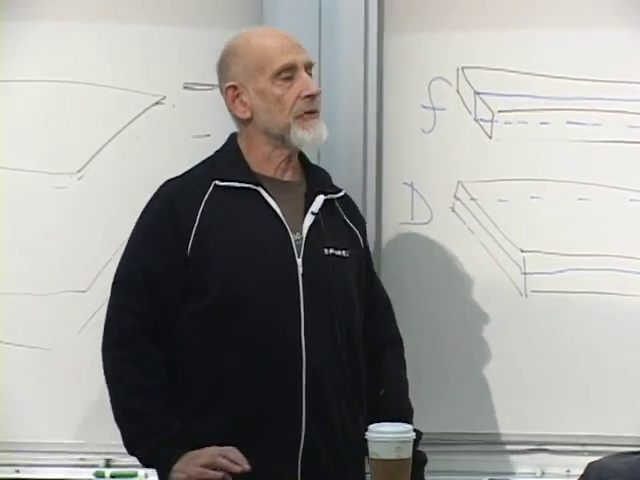
\includegraphics[width=0.78\textwidth]{lecture_01_figure_03.png}
\lectureframe{01:10:25.000}
\caption{二つの巻き付いた膜について完成した黒板の状態。短いコンパクトサイクルと長いコンパクトサイクルは、右に描かれたF弦およびD弦のようなリボンを生じる。}
\end{figure}

膜はどちらのコンパクト方向にも巻き付くことができ、非コンパクト方向から見ると弦のように見える。\(R_1\)と\(R_2\)が二つの円の半径であるなら、その有効張力は
\begin{equation}
\begin{aligned}
T_{(1)}&=2\pi R_1 T_{\mathrm{M2}},\\
T_{(2)}&=2\pi R_2 T_{\mathrm{M2}},\\
\frac{T_{(1)}}{T_{(2)}}&=\frac{R_1}{R_2}.
\end{aligned}
\end{equation}
したがって、等しくない円の大きさは等しくない弦の張力を生じる。短い方への巻き付きを軽いF弦、長い方への巻き付きを重いD弦と同定すると、概略的に
\begin{equation}
g_s\sim \frac{R_{\mathrm{short}}}{R_{\mathrm{long}}},
\qquad
\frac{T_{\mathrm{D1}}}{T_{\mathrm{F1}}}\sim \frac{1}{g_s}.
\end{equation}
と書ける。

\begin{classroomqa}
\audiencequestion{この描像における結合定数は、二つのコンパクト次元の比として理解できるか。\lecturetimestamp{01:10:13}}
\lecturerresponse{はい。弱--強パラメータはアスペクト比として幾何化される。一方の方向を短くすると小さな結合定数が生じ、二つの方向を交換すると軽い弦と重い弦が交換される。}
\end{classroomqa}

\editorialnote{講義では一時的にこの比を\(\alpha\)と呼び、以前にQEDの微細構造定数に用いた記号を再利用している。ここでは二つの意味を区別しておくために\(g_s\)と書く。完全なM理論の構成では、IIB型の結合定数はコンパクトな二次元トーラスの複素構造に符号化されており、正確な分子はそのサイクルをどのようにラベル付けするかに依存する。}

巻き付いた膜の描像は、黒板の絵の遠近の歪みなしに次のように要約できる。

\begin{figure}[htbp]
\centering
\begin{tikzpicture}[scale=1.0]
\draw[line width=0.9pt] (0,0) rectangle (5.2,2.2);
\node[below] at (2.6,-0.2) {\(R_1\)};
\node[right] at (5.4,1.1) {\(R_2\)};

\draw[->,line width=0.7pt] (5.45,1.9) -- (5.45,0.3);
\draw[->,line width=0.7pt] (5.7,0.3) -- (5.7,1.9);
\draw[->,line width=0.7pt] (0.4,-0.35) -- (4.8,-0.35);
\draw[->,line width=0.7pt] (4.8,-0.6) -- (0.4,-0.6);

\draw[line width=1.0pt] (1.1,0) -- (1.6,0) -- (1.6,2.2) -- (1.1,2.2) -- cycle;
\node at (1.35,2.55) {light};

\draw[line width=1.0pt] (0,1.45) -- (5.2,1.45);
\draw[line width=1.0pt] (0,1.00) -- (5.2,1.00);
\node at (4.55,1.95) {heavy};

\node at (1.35,-0.95) {F-string};
\node at (4.55,0.55) {D-string};
\end{tikzpicture}
\caption{二つの巻き付いた膜の配置はどちらも非コンパクト方向からは弦のように見えるが、等しくないコンパクトなスケールのために一方の有効な弦が他方より軽くなる。}
\end{figure}

これは以前の双対性の話の幾何学的な版である。一方の方向を圧縮し他方を伸ばすと、一方の巻き付いた対象が重くなり他方が軽くなるので、F弦とD弦の役割は入れ替わりうる。

\begin{classroomqa}
\audiencequestion{コンパクト方向が周期的であるなら、巻き付いた対象は無限に広いのか。\lecturetimestamp{01:10:41}}
\lecturerresponse{いいえ。コンパクトな円は、端に達することなく繰り返し周回できるとしても、有限の円周をもつ。切り開いた絵の上端と下端は同じ点を表し、ちょうど区間の端点が一つの円の点を表しうるのと同じである。}
\end{classroomqa}

\begin{figure}[htbp]
\centering
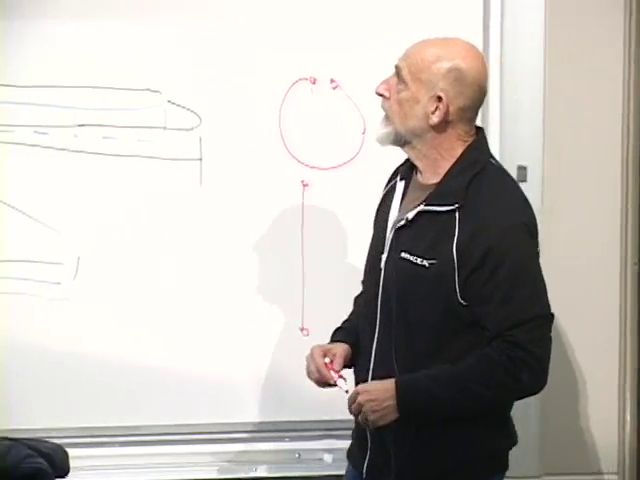
\includegraphics[width=0.78\textwidth]{lecture_01_figure_04.png}
\lectureframe{01:12:25.000}

\vspace{1em}

\begin{tikzpicture}[scale=0.95]
\draw[line width=0.9pt,->] (-3.7,0) arc[start angle=180,end angle=535,radius=0.95];
\node at (-2.75,0) {compact circle};
\draw[line width=0.9pt] (0.0,0) -- (4.8,0);
\fill (0.0,0) circle (0.06);
\fill (4.8,0) circle (0.06);
\draw[<->] (0.0,-0.45) -- (4.8,-0.45);
\node at (2.4,-0.75) {cut-open interval of length \(2\pi R\)};
\node[above] at (0.0,0.1) {same point};
\node[above] at (4.8,0.1) {same point};
\end{tikzpicture}
\caption{コンパクトな円とその切り開いた黒板表示。一方の端点を越えると他方で戻る。円の周りを進みながら同時に非コンパクト方向にも進むなら、代わりに螺旋を描くであろう。}
\end{figure}

\begin{classroomqa}
\audiencequestion{なぜコンパクトな経路は螺旋ではなく円なのか。\lecturetimestamp{01:12:23}}
\lecturerresponse{非コンパクト方向の各固定点において、コンパクト方向は円である。螺旋は、非コンパクト方向に進みながら同時に円の周りを巻く場合にのみ現れる。黒板上の区間は単に切り開かれた円であり、その二つの端点は同一視されている。}
\end{classroomqa}

\begin{classroomqa}
\audiencequestion{この幾何学自体が、Dブレーンが近くから調べられたときにどのようにF弦の集まりのように見えうるかを説明するのか。\lecturetimestamp{01:12:49}}
\lecturerresponse{関連は存在するが、この初等的な描像では透明ではない。それを見るにはより多くの幾何学的な道具立てが必要である。この図は双対性を整理するためのものであり、あらゆる微視的な構成要素の記述を導出するためのものではない。}
\end{classroomqa}

\begin{classroomqa}
\audiencequestion{長いコンパクト方向と短いコンパクト方向は、空間を移動するにつれて、あるいは時間が進むにつれて交換しうるか。\lecturetimestamp{01:13:35}}
\lecturerresponse{理想化された模型ではどちらも可能である。一方のサイクルを潰し他方を膨張させると、どちらの巻き付いた弦が軽いかが入れ替わる。これは``基本弦''が単なる名前であるもう一つの理由である。好ましい記述は領域ごとに、あるいは時間とともに変化しうる。}
\end{classroomqa}

\section{理想化、特別に対称な点、そしてランドスケープ}

講義の最後の楽章は、優雅な双対性の例から一歩引いて、それらが現実世界について何を語り、何を語らないのかを問う。

まず、Susskindは、精密に制御された双対性は高度に理想化された超対称理論の特徴であり、そこではボソンとフェルミオンが正確に一致した質量で現れると警告する。彼の類推はニュートン力学における円軌道である。実際の惑星運動が完全な円で尽くされるからではなく、対称で数学的に扱いやすいから、まずそれを研究するのである。まったく同じように、超対称弦理論は、自然が示すよりも対称性が高いため、解析しやすいのである。

それでもこの理想化は有益である。完全な円軌道は現実的な惑星系ではないが、より対称性の低い軌道にも生き残る特徴を表している。同様に、超対称な例は、量子力学、重力、微視的構造が整合的に共存しうる仕方を示している。Susskindの意図的に鋭い定式化によれば、扱いやすい弦理論は文字通り我々の世界の理論ではない。その価値は、より対称性が低く扱いにくい設定で再び現れそうな現象を明らかにすることにある。

\subsection{多くの結果をもたらす構成キット}

Dブレーンは利用可能な構成キットの一部にすぎない。講義ではフラックス、オービフォールド、オリエンティフォールドも挙げられている。まずコンパクトな幾何学を選び、次にどのブレーンとフラックスがそのサイクルを占めるかを選ぶ。単純なサンドイッチでさえ、浮遊するD2ブレーンを1枚、2枚、あるいは3枚挿入すると、その低次元物理を変える。そのような要素を加えたり減らしたりすると、有効な粒子、相互作用、パラメータが変化する。

講義の概略的な数え方で、6次元コンパクト空間がおよそ\(500\)個のサイクルを持ち、各サイクルが巻き付いたブレーン、フラックス、または関連する構造の\(10\)通りの選択を許すとしよう。すると構成の数は次のように増大する。
\begin{equation}
N_{\mathrm{vacua}} \sim 10^{500}.
\end{equation}
講義の数え方の論理は初等的である。
\begin{equation}
10 \times 10 \times \cdots \times 10 = 10^{500}
\end{equation}
ここで\(500\)個の因子がある。DNAの類推は同じ点をより身近な調子で述べている。
\begin{equation}
N_{\mathrm{DNA}}(500)=4^{500}.
\end{equation}
DNAの比較の際、聴衆の一人が一本の鎖に沿って4つの選択肢、A、C、G、Tがあることを確認する。この訂正は議論を変えるのではなく、むしろ補強する。局所的な選択の短いリストが何度も繰り返されることで、膨大な数の大域的配置が生じる。正確な指数が要点ではなく、Susskindは\(10^{500}\)を古い過小評価と呼んでいる。要点は組合せ論的な急増である。

これは冒頭の還元主義的期待の最終的な反転を与える。複雑な素粒子物理学は複雑な微視的規則から生じる必要はない。ちょうど複雑な生物が4つの塩基から作られた配列によって符号化されうるように、我々の真空が多くの単純な要素からなる一つの複雑な配置であるために生じうるのである。

\begin{classroomqa}
\audiencequestion{双対性で結ばれた等価な記述を同一視した後、完全な情報は、我々の世界の記述としてこれらの可能な真空のうちただ一つまたは少数だけを選び出すのだろうか。\lecturetimestamp{01:26:11}}
\lecturerresponse{おそらく制限された集合を選び出すだろうが、多くの異なる真空が到達可能なエネルギーでは極めて似て見えるかもしれない。引用されたランドスケープの数は、双対な記述を同一視した後でも依然として大きいままであり、無関係な高エネルギー的詳細は``ジャンクDNA''}のように機能しうる。\end{classroomqa}

\subsection{対称な点と一般的な複雑さ}

ランドスケープの中には特別に対称な点がある。幾何学的な描像では、等アスペクト配置
\begin{equation}
R_1=R_2,
\end{equation}
は二つの巻き付いた記述を等しく単純にする。電気--磁気の類推では、これは模式的に次で表される。
\begin{equation}
m_{\mathrm{monopole}}=m_e.
\end{equation}

\begin{figure}[htbp]
\centering
\begin{tikzpicture}[scale=0.95]
\draw[line width=0.9pt] (-4.5,-1.0) rectangle (-2.5,1.0);
\draw[<->] (-4.5,-1.35) -- (-2.5,-1.35);
\draw[<->] (-2.15,-1.0) -- (-2.15,1.0);
\node at (-3.5,1.45) {symmetric point};
\node at (-3.5,-1.75) {$R_1=R_2$};

\draw[line width=0.9pt] (0.0,-0.55) rectangle (4.8,0.55);
\draw[<->] (0.0,-0.9) -- (4.8,-0.9);
\draw[<->] (5.15,-0.55) -- (5.15,0.55);
\node at (2.4,1.45) {lopsided point};
\node at (2.4,-1.3) {$R_1\ne R_2$};
\end{tikzpicture}
\caption{等アスペクトのコンパクト化は二つの巻き付いた弦を対称に扱い、偏ったコンパクト化は一方の記述を他方よりずっと軽くする。}
\end{figure}

\begin{classroomqa}
\audiencequestion{F弦とD弦の記述が一致するために構成がずっと単純になるような真空がランドスケープの中にあるのだろうか。\lecturetimestamp{01:27:21}}
\lecturerresponse{はい、特別に対称な点はある。我々の世界はそのような点に位置しているようには見えない。身近な電気的粒子と磁気単極子は等しい質量を持たない。なぜ自然が偏った点を占めるのかは知られていない。}
\end{classroomqa}

\editorialnote{電子--モノポールの質量が等しいことは、適切に保護された自己双対模型の模式的な特徴であり、通常の超対称性のない量子電磁力学の予言ではない。これは観測された電子についての主張ではなく、講義における対称点の考え方を表している。}

サスキンドは次に、通信理論からの類推を思い起こす。ランダム符号は極めて優れたものになり得る一方、最も記述しやすく復号しやすい符号は余分な数学的構造を持ち、歴史的には性能が劣っていた。符号理論は後に非常に効果的な構造化された構成を発見したが、類推はなお残る。すなわち、簡潔に名づけられ、あるいは記述されるものは、可能なもの全体の空間の中でも非常に特別な、低複雑性の隅を占める。同様に、最も計算しやすい弦真空は、典型的でないほど単純かもしれない。

したがって、適切な問いは変わり得る。あらゆる微視的細部において厳密なコンパクト化を要求する代わりに、広いアンサンブルにわたってどの特徴が共通であるか、あるいは一般的であるかを問うことができる。サスキンドはこれを、決着した結論ではなく研究課題として提示し、計算の代わりにイデオロギー的議論を退ける。

\subsection{宇宙論的問い}

\begin{classroomqa}
\audiencequestion{巨大な円周を持つコンパクトな方向は、無限の方向と観測上異なるのか、また、我々の三つの大きな空間次元が無限であることを我々は知っているのか。\lecturetimestamp{01:30:03}}
\lecturerresponse{それらが無限であることは知られていない。閉じた三次元球面は、コンパクトでありながら膨張することができる。ほぼ平坦であることの測定は、曲率半径に関する下限を与えるにすぎない。ちょうど、ほぼ平坦な土地を測量しても、地球の表面が無限であることを証明せずに地球の大きさを制限できるのと同じである。検出された曲率または大域的識別だけが、有限のスケールを決定するであろう。}
\end{classroomqa}

\begin{classroomqa}
\audiencequestion{理想化された模型において結合が空間を通じて変動し得るなら、そのような変動は現実世界でどのように起こり得るのか。\lecturetimestamp{01:32:43}}
\lecturerresponse{対称的な例で用いられた無制限の滑らかな変動としてではない。後に論じられる現実的な可能性は、異なる有効法則を持つ領域間の離散的遷移による変動である。そのような跳びが起こるかどうかは宇宙論的問いである。}
\end{classroomqa}

\editorialnote{この応答は、あらゆる滑らかに変動するスカラー場を禁じる一般的定理としてではなく、フラックス真空と領域遷移についての講義の予告として読まれるべきである。観測は無次元結合の変動を強く制限する一方、安定化機構は、与えられた模型において連続的モジュライが利用可能なままであるかどうかを決定する。}

録音は最後の聴衆からの質問を保存していない。残っている応答は、提案された現象がある種のブラックホールについては起こり得るが、通常のシュヴァルツシルト・ブラックホールの事象の地平面では起こらない、と言っている。その地平面は、自由落下する観測者にとって局所的には普通の場所である。質問を信頼できる形で復元できないため、このやり取りにこれ以上具体的な主張は帰されない。

\section{レンガから記述の網へ}

物理学のより深い層はより単純でなければならないという希望は、もろいものと判明した。\(1+1\)次元のボソン化では、同じ理論をフェルミオンを中心に組織することも、ボソンを中心に組織することもでき、フェルミオンはキンクとして再現する。量子電気力学では、弱結合と強結合が電子と磁気単極子の記述的役割を交換する。弦理論では、F弦とD弦が同じパターンを繰り返し、偶数ブレーン理論では強結合はさらに進む。コンパクトな方向が膨張し、D0ブレーンがKaluza--Klein運動量状態となり、有効弦がより高次元の幾何学における巻き付いた膜として再解釈される。したがって、現代の量子場の理論と弦理論は、``どちらがレンガでどちらが家か''という問いに対して、唯一の最終的な答えを与えるものではない。それらは、それぞれが自らの領域で効率的である記述の網と、可能な構成の巨大な景観とを与える。その一般的な出力は単純さではなく複雑さである。

\chapter{幾何学、情報、そしてブラックホールの面積則}

\lectureoverview{宣言された目的地は宇宙論であるが、そこへの最短の道は特殊相対性理論への回帰から始まる。計量は時空の幾何学を教え、固有時間がゼロであるという条件は光がどのように運動するかを教える。この一つの規則をシュヴァルツシルト幾何学へと持ち込み、事象の地平面と特異点を区別し、そしてブラックホールが放射によって蒸発するとき情報はどうなるのかを問う。その答えは通常のエントロピーから始まり、ベッケンシュタインの1ビットの議論で終わる。すなわち、ブラックホールは体積ではなく地平面の面積を単位として情報を蓄えるのである。}

ススキンドは、弦理論の成功と失敗について約束した会計をしばらく延期する。彼によれば、時間が遅く、また監査よりも実質の方が有用である。今夜の実質とは、ブラックホール情報問題を定式化するために必要な最小限の幾何学と熱力学である。

\section{光に対する一つの規則}

特殊相対性理論は空間と時間を一つの幾何学的対象として扱う。\(dt,dx,dy,dz\)だけ離れた隣接する事象に対して、ススキンドは主にマイナスの符号の規約を用いて次のように書く。
\begin{equation}
d\tau^2=dt^2-\frac{1}{c^2}\left(dx^2+dy^2+dz^2\right).
\end{equation}
時間的部分と空間的部分の符号が反対であることが、ミンコフスキー幾何学を4次元ユークリッド幾何学から区別する。因子\(1/c^2\)は単に単位を調和させるだけであり、時間と距離を整合的に測ることにより\(c=1\)と置くことができる。

時間的隔たりでは\(d\tau^2>0\)であり、\(d\tau\)はその軌道に従う時計が記録する固有時間である。空間的隔たりでは代わりに\(d\tau^2<0\)となる。今夜必要となる場合はちょうどその中間にある。光線は\emph{ヌル}な軌道に従い、
\begin{equation}
d\tau^2=0.
\end{equation}
まず\(x\)軸に沿った運動に制限すると、
\begin{align}
0&=dt^2-\frac{dx^2}{c^2},\\
c\,dt&=\pm dx,\\
\frac{dx}{dt}&=\pm c.
\end{align}
符号は右向きおよび左向きの光線を表す。\(c\)に割り当てられる数値は、センチメートルをメートルやキロメートルに置き換えると変化する。不変な言明は数ではなく、ヌル条件である。

一般相対性理論が複雑にするのは計量であって、この規則ではない。座標\(x^\mu\)、\(\mu=0,1,2,3\)を用いると、
\begin{equation}
ds^2=g_{\mu\nu}(x)\,dx^\mu dx^\nu,
\end{equation}
ここで繰り返された添字は和をとり、係数は点ごとに変化しうる。光が局所的に許される方向を見つけるには、この二次形式をゼロと置けばよい。

\section{球座標とシュヴァルツシルト計量}

回転しないブラックホールは球対称であるため、デカルト座標は有用な構造を隠してしまう。\(r\)を動径距離とし、\(\theta,\phi\)を単位球面上の方向を指定するものとしよう。その線素は
\begin{equation}
d\Omega^2=d\theta^2+\sin^2\theta\,d\phi^2.
\end{equation}
である。半径\(r\)の球面上では、角度の変位はしたがって\(r^2d\Omega^2\)に寄与する。球座標における平坦な時空は
\begin{equation}
d\tau^2=dt^2-\left(dr^2+r^2d\Omega^2\right),
\qquad (c=1).
\end{equation}
である。

ススキンドはアインシュタイン方程式からブラックホール解を導出しない。彼はそれを書き下し、我々にそれを吟味するよう求める。黒板は意図された比較を明示する。

\begin{figure}[htbp]
\centering
\includegraphics[width=0.86\textwidth]{lecture_02_figure_02.png}
\caption{上は平坦な球面時空、下はシュヴァルツシルトの変形。繰り返される因子\(1-2GM/(c^2r)=1-R_s/r\)と動径方向のスケッチが一緒に見える。}
\lectureframe{00:19:12.520}
\end{figure}

質量\(M\)のブラックホールに対して、シュヴァルツシルト半径を
\begin{equation}
R_s=\frac{2GM}{c^2}.
\end{equation}
と定義する。外部の線素は
\begin{equation}
d\tau^2=\left(1-\frac{R_s}{r}\right)dt^2
-\frac{dr^2/c^2}{1-R_s/r}
-\frac{r^2}{c^2}d\Omega^2.
\label{eq:schwarzschild-explicit-c}
\end{equation}
である。等価に、\(c=1\)と置いた後では、
\begin{equation}
ds^2=\left(1-\frac{2GM}{r}\right)dt^2
-\frac{dr^2}{1-2GM/r}-r^2d\Omega^2.
\label{eq:schwarzschild}
\end{equation}
となる。遠方では\(R_s/r\ll1\)であり、平坦な球面計量が戻ってくる。この漸近的検査は公式を暗記することよりも重要であるが、ススキンドは後者をカクテルパーティーの材料として推奨している。

\editorialnote{黒板は\(d\tau^2\)と\(ds^2\)の間で交互に切り替わり、\(c\)のすべての因子を一貫して表示しているわけではない。式~\eqref{eq:schwarzschild-explicit-c}は講義の時間座標の規約に従っており、そこでは\(t\)は時間の単位を持つ。\(x^0=ct\)を用いた標準的な形は代数的に等価である。}

\subsection{地平面は特異点ではない}

座標の中で二つの半径が怪しく見える。自然単位で\(r=R_s=2GM\)では、\(dt^2\)の係数が消え、\(dr^2\)の係数が発散する。\(r=0\)では、曲率自体が特異になる。これらは同じ事象の二つの版ではない。
\begin{equation}
\begin{aligned}
r=R_s &:\quad \text{horizon},\\
r=0 &:\quad \text{curvature singularity}.
\end{aligned}
\end{equation}

潮汐力が物理的な区別を与える。重力場は広がりを持つ物体の各部で異なる。すなわち、足は頭よりも強く引かれ、物体を引き伸ばす一方で横方向は圧縮される。地平面ではそれらの潮汐力は有限であり、十分に大きな質量のブラックホールの地平面では非常に小さくなりうる。そこでは局所的に破局的なことは何も起こる必要がない。対照的に\(r=0\)では、潮汐力は発散する。\(r=R_s\)における警告的な係数はシュヴァルツシルト座標の欠陥を告げている。\(r=0\)の特異点は物理的である。

\editorialnote{曲率が\(r=R_s\)で有限であることは、Kretschmannスカラー\(R_{\mu\nu\rho\sigma}R^{\mu\nu\rho\sigma}=48G^2M^2/(c^4r^6)\)から確認できる。これは事象の地平線で有限であり、\(r\to0\)でのみ発散する。この不変量は講義では書かれなかったが、潮汐力の区別を精密にするものである。}

\section{地平線近傍の動径方向の光}

ここで一つの規則に戻る。動径方向の光線は角位置を固定したままであるから、\(d\Omega=0\)であり、光線では\(ds^2=0\)である。\(c=1\)単位では、式~\eqref{eq:schwarzschild}より
\begin{equation}
0=\left(1-\frac{2GM}{r}\right)dt^2
-\frac{dr^2}{1-2GM/r}.
\end{equation}
\(1-2GM/r\)を掛けて平方根をとると二つの分枝が得られる。
\begin{align}
dr&=\pm\left(1-\frac{2GM}{r}\right)dt,\\
\frac{dr}{dt}&=\pm\left(1-\frac{2GM}{r}\right).
\label{eq:radial-null}
\end{align}
プラス符号は外向き、マイナス符号は内向きである。遠方ではそれらの座標速度は\(\pm1\)に近づく。地平線では両者とも\(\lvert dr/dt\rvert\to0\)を満たす。すなわち、Schwarzschild座標時間では、外向き光線はそこで静止しているように見え、内向き光線は到達するのに無限の座標時間を要する。

\begin{figure}[htbp]
\centering
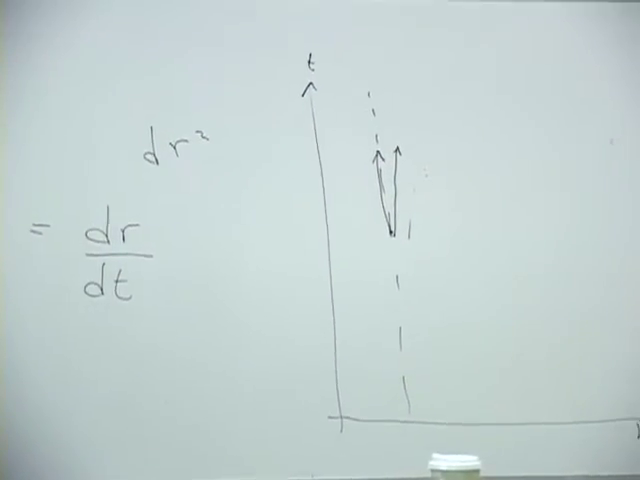
\includegraphics[width=0.82\textwidth]{lecture_02_figure_03.png}
\caption{完成した\(t\)-\(r\)黒板スケッチ。破線の地平線に近づくにつれて、動径方向のヌル光線はほぼ垂直になる。}
\lectureframe{00:30:25.000}
\end{figure}

\begin{figure}[htbp]
\centering
\begin{tikzpicture}[x=1.0cm,y=0.9cm]
\draw[->] (0,0) -- (6.6,0) node[right] {$r$};
\draw[->] (0,0) -- (0,6.2) node[above] {$t$};
\draw[dashed,thick] (2.0,0) -- (2.0,5.9) node[above] {$r=R_s$};
\draw[thick,->] (2.08,.4) .. controls (2.10,2.2) and (2.55,3.8) .. (5.8,5.7);
\draw[thick,->] (5.8,.5) .. controls (3.2,2.0) and (2.15,4.2) .. (2.03,5.7);
\node[align=center] at (4.7,4.4) {outgoing};
\node[align=center] at (4.5,1.2) {ingoing};
\end{tikzpicture}
\caption{黒板スケッチを座標時間で整理した版。見かけの減速はSchwarzschild\(t\)についての記述であり、光が\(c\)で進むことの局所的な破綻についてのものではない。}
\end{figure}

地平線の内側では、未来光円錐が内側へ大きく傾き、未来向きの動径方向の両分枝が\(r\)の減少へ向かう。そこから出発した信号は外部へ脱出できず、未来向きの因果的経路はすべて特異点に到達する。

\begin{classroomqa}
\audiencequestion{光速度が不変であるなら、地平線近くで光が減速すると言うことは正確には何を意味するのか。\lecturetimestamp{00:31:44}}
\lecturerresponse{表示された量は、特定の座標系における\(dr/dt\)である。数値的な速度は、メートルをセンチメートルに置き換えただけでもすでに変化する。ここでは、有効な動径方向と時間方向の目盛りが位置によって変わる。普遍的な言明は、すべての光線がヌル軌道\(ds^2=0\)に従うということである。}
\end{classroomqa}
\editorialnote{自由落下する局所観測者は真空中の光を\(c\)と測定する。地平線でSchwarzschild座標速度が消えることは局所的な観測量ではない。}

\begin{classroomqa}
\audiencequestion{光が通る物質媒質にかかわらず、同じヌル速度の言明が成り立つのか。\lecturetimestamp{00:33:24}}
\lecturerresponse{成り立たない。利用可能な認識は、もはやこの答えの説明を保持していない。}
\end{classroomqa}
\editorialnote{ヌル速度の主張は、真空時空における伝播に関するものである。物質との相互作用は波束に小さな有効速度を与えうるが、それは媒質の性質であり、局所的な因果速度\(c\)の変化ではない。}

\begin{classroomqa}
\audiencequestion{同じ\(t\)-\(r\)図で、入射する光線はどのように見えるか。\lecturetimestamp{00:33:32}}
\lecturerresponse{それは逆向きに見える分枝である。大きな\(r\)から地平線へ曲がり、漸近的に近づく。到達するには無限の座標時間\(t\)を要する。}
\end{classroomqa}
\editorialnote{落下する観測者は有限の固有時間で地平線に到達し、それを横切る。発散するのはSchwarzschild\(t\)のみである。}

\section{なぜ蒸発が問題を生むのか}

地平線はさらに多くの研究に値する。どのように形成されるか、落下する観測者に何が見えるか、そこで局所的に異常なことが起こるかどうかである。Susskindはこれらの問いを後回しにし、量子力学へと跳ぶ。外部から見ると、物質とその識別情報のすべてはますます地平線近くに押し込められ、利用できなくなる。それだけでは情報を破壊する必要はない。単に隠しているだけかもしれない。

Hawkingの結果はこの問題を深刻にする。落ち着いた古典的黑洞は、想像しうる最も退屈な物体のように見える。球対称で、暗く、メッセージを送ることができない。しかし``black''には二つの意味がある。何も放出しないという意味にもなりうるし、熱的な黒体放射を放出するという意味にもなりうる。量子的な黑洞は第二の意味で黒い。温度を持ち、輝き、エネルギーを失う。
\begin{equation}
E=Mc^2,
\qquad
R_s=\frac{2GM}{c^2},
\end{equation}
であるから、放射はその質量と地平線半径の両方を減少させる。蒸発が最終的に黑洞を消し去るなら、その地平線に残っているように見えた情報はどうなるのか。それは破壊されるか、小さな残骸に閉じ込められるか、外向き放射に符号化されるかもしれない。これらの可能性の間の緊張が情報問題であり、弦理論は後にその解決を鋭くする助けとなるであろう。

今夜は曲がった時空における量子場の計算は試みない。代わりにSusskindはBekensteinのより単純な道をたどる。まずエントロピーを情報として理解し、次に黑洞がどれだけの情報を隠せるかを計算する。

\section{存在するが隠されている情報}

箱を、各セルが占有されているか空であるかのどちらかになるほど小さなセルに分割することを想像しよう。二値文字列---セルごとに一つの答え---は、その配置を他のすべての許された配置から区別する。より現実的な物質では、粒子の種類や他の自由度についての問いが必要になるが、原理は変わらない。情報は、状態を指定するために必要なはい--いいえの問いの最小数によって測られる。

\begin{classroomqa}
\audiencequestion{これは静的な系の記述にすぎないのですか。\lecturetimestamp{00:45:49}}
\lecturerresponse{これはある1つの時刻における瞬間的な記述である。その後、力学がその状態を別の状態へ写す。}
\end{classroomqa}

次の原理はより深い。閉じた系の時間発展は、2つの異なる微視的状態を1つに融合しない。2つの配置が現在異なっているなら、それらが時間発展した配置も原理的には区別可能なままである。古典的ハミルトン時間発展は可逆であり、量子時間発展はユニタリである。\editorialnote{散逸的な有効方程式が区別を消し去ることができるのは、観測されない環境の自由度が省略されているからにすぎず、完全な閉じた状態はそれらを保持している。}

浴槽は、損失と到達不能性の違いを具体的にする。2つの水滴の流れは、2つの異なるモールス符号のテキストを符号化しうる。水が落ち着いた後、両方の浴槽は同じに見える。目に見える波紋は消えたが、完全な微視的測定を行えば、依然として異なる分子配置が見出されるであろう。メッセージは、追跡するには小さすぎ、多すぎる自由度へと広がってしまったのである。

エントロピーとは、この隠れた情報のことである。我々が問うことのできる巨視的な問い---温度、全エネルギー、組成、水位---に対して、多くの微視的区別は可能なままだが到達不能である。講義のビット数え上げの言葉では、
\begin{equation}
S=\hbox{number of hidden bits}.
\end{equation}
厳密な統計的公式は\(S=k_B\ln\Omega\)であるが、定性的な定義でブラックホールの議論には十分である。

\section{ビットを隠すコストとしての温度}

温度は測定するのは身近だが、定義するのは驚くほど間接的である。サスキンドはエントロピーとエネルギーを原始的な概念として選ぶ。コンピュータのビットが標準的な値にリセットされると仮定しよう。物理的デバイスは残るが、以前の0と1の状態の区別はコンピュータから消える。それは完全な世界から消えることはできず、環境の微視的自由度に移され、それらをわずかに加熱する。これがランダウアーの原理である。

1エントロピー単位が1ビットであり、温度がエネルギー単位で測られるなら、講義は次のように書く。
\begin{align}
\Delta S&=1,\\
\Delta E&=T\,\Delta S,\\
dE&=T\,dS.
\label{eq:first-law}
\end{align}

\begin{figure}[htbp]
\centering
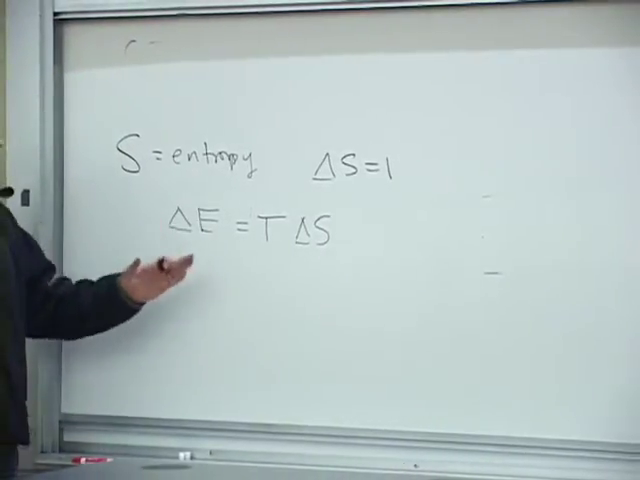
\includegraphics[width=0.84\textwidth]{lecture_02_figure_04.png}
\caption{黒板の情報理論的热力学：\(S\)はエントロピーであり、1つの隠れたビットは\(\Delta S=1\)を持ち、その最小エネルギーコストは\(\Delta E=T\Delta S\)と書かれる。}
\lectureframe{00:58:40.000}
\end{figure}

\editorialnote{従来の単位では、1つの二進ビットの可逆的消去コストは\(k_BT\ln2\)である。式~\eqref{eq:first-law}は\(k_B=1\)を用い、講義のエントロピー単位を1ビットとして扱い、関連する\(\ln2\)を抑制している。これらの規約は、続くスケーリングの議論には影響しない。}

ある聴衆による見積もりでは、およそ\(100\)ギガバイトを消去することによる最低温度上昇は、コップ一杯の水でおよそ\(10^{-15}\)度である。サスキンドは正確な数値ではなく、その要点を受け入れる。室温では1ビットが運ぶ最小エネルギーは極めて小さく、実際のコンピュータは消去が可逆的に行われないためにはるかに多くを散逸する。

\begin{classroomqa}
\audiencequestion{ハードドライブの例は単なる類推なのか、それとも消去による加熱は実際の法則なのか。\lecturetimestamp{01:00:02}}
\lecturerresponse{それは実際の物理的制約、すなわちランダウアーの規則である。メモリセルをリセットすると、古い区別がコンピュータから取り除かれ、その情報は環境へ運ばれなければならない。通常の操作は、回路を駆動し、電荷を移動させ、無関係な熱を生み出すため、理想的な最小値よりもはるかに効率が悪い。}
\end{classroomqa}

\begin{classroomqa}
\audiencequestion{1ビットを隠すコストは、より高い温度ではより多くのエネルギーを要しますか。\lecturetimestamp{01:02:07}}
\lecturerresponse{はい。関係\(dE=T\,dS\)はまさにそのことを述べている。同じエントロピー移動に対して、より熱い熱浴はより大きなエネルギー移動を必要とする。この隠れたビットあたりのエネルギー関係を温度の定義と見なすことも同様にできる。}
\end{classroomqa}

\begin{classroomqa}
\audiencequestion{以前に保存されたビットに上書きした場合、その古い情報は失われたのですか。\lecturetimestamp{01:02:43}}
\lecturerresponse{それはコンピュータから去ったが、閉じた物理系から消え去ったわけではない。上書きされた区別は環境へと分散され、そこで到達不能な情報として寄与し、したがってエントロピーに寄与する。}
\end{classroomqa}

熱力学的エントロピーを失われた微視的情報と同一視する見方はボルツマンにさかのぼる。シャノンは20世紀に対応する情報理論的な言語を与えた。ススキンドは、彼と聴衆の一部が1950年代に出会った熱力学の講義では、この説明が不思議なほど欠けていたと述べている。計算機科学によってこの結びつきは見落としにくくなったが、その物理的内容を生み出したわけではない。

\section{ブラックホールに1ビットを入れる}

今や、浴槽に一滴ずつ水を注ぐように、概念上ビットを一つずつ加えてブラックホールを構成できる。問題は微分形である。追加の1ビットが隠されたとき、事象の地平面はどれだけ成長するか。質量\(M\)、半径\(R_s\)の穴から始め、回収可能な区別が吸収されたかどうかだけである最も単純な物体を送り込む。

\begin{classroomqa}
\audiencequestion{情報が穴に入るには無限の座標時間が必要ではないのか。\lecturetimestamp{01:08:07}}
\lecturerresponse{それは地平面近傍で指数的に圧縮され、実際の短い時間のうちに外部から利用できなくなる。ただしシュヴァルツシルト座標時間では実際の横断に無限の値が割り当てられる。したがって外部の会計としては、地平面に蓄えられているとみなしてよい。}
\end{classroomqa}

光子は自然な候補であるが、一般的な光子は一ビットより多くの情報を運ぶ。その偏光は二値的な選択を符号化しうる。鋭く局在した到達点は、さらに多くのイエス--ノーの問いを与える。上半球か下半球か、左半分か右半分か、などである。量子力学は局在をおよそ一波長に制限するので、位置情報を抑える方法は、穴がなお吸収できる最長の波長を用いることである。

\begin{classroomqa}
\audiencequestion{光子が入ることのできない上限波長が本当にあるのか。\lecturetimestamp{01:12:15}}
\lecturerresponse{はい。穴よりずっと大きな波は、吸収されるよりも主に散乱される。有用な限界的選択は、地平面半径と同程度の波長である。すなわち、入射点をぼかすのに十分長く、しかも実質的な吸収確率をもつのに十分短い。}
\end{classroomqa}

\begin{classroomqa}
\audiencequestion{光子が到来する方向自体が情報を加えるのか。\lecturetimestamp{01:13:28}}
\lecturerresponse{波長が地平面全体程度であれば、場は穴を横切って非常にゆっくり変化するので、到来方向を細かい精度で分解できない。これが、長波長極限が鋭く局在した衝突ではなく単一のイエス--ノーのデータに近似的に対応する理由である。}
\end{classroomqa}

したがって桁の程度で次を選ぶ。
\begin{equation}
\lambda\sim R_s=\frac{2GM}{c^2}.
\label{eq:one-bit-wave}
\end{equation}
光子の運動学から次が得られる。
\begin{equation}
E=cp,
\qquad
p=\hbar k=\frac{h}{\lambda},
\qquad
\Delta E\sim\frac{\hbar c}{R_s}.
\label{eq:one-bit-energy}
\end{equation}
ここで\(k=2\pi/\lambda\)および\(h=2\pi\hbar\)である。この講義では\(2\pi\)を意図的に無視し、1次の吸収因子も同様に無視する。

\begin{classroomqa}
\audiencequestion{運動量は\(\hbar/\lambda\)と書くべきか、それとも\(h/\lambda\)か。\lecturetimestamp{01:16:00}}
\lecturerresponse{\(\lambda\)を通常の波長とすると、厳密な関係は\(p=h/\lambda=2\pi\hbar/\lambda\)である。波数\(k=2\pi/\lambda\)を用いれば\(p=\hbar k\)である。ここでの見積もりはスケールのみを保つので、因子\(2\pi\)は意図的に捨てられる。}
\end{classroomqa}

1ビットを隠すエネルギーのコストは温度スケールである。したがって式~\eqref{eq:one-bit-wave}と~\eqref{eq:one-bit-energy}から次が得られる。
\begin{equation}
k_BT_H\sim\frac{\hbar c}{R_s}
\sim\frac{\hbar c^3}{GM}.
\end{equation}
厳密なホーキングの結果は次である。
\begin{equation}
k_BT_H=\frac{\hbar c^3}{8\pi GM}.
\end{equation}
初等的な議論は\(M,G,c,\hbar\)への依存性は得るが、係数は得ない。

\section{1ビットは1プランクスケールのパッチを占める}

同じ光子が地平面の成長の仕方を教えてくれる。そのエネルギーは質量を次だけ変える。
\begin{equation}
\Delta M=\frac{\Delta E}{c^2}
\sim\frac{\hbar}{cR_s}.
\end{equation}
\(R_s=2GM/c^2\)なので、
\begin{equation}
\Delta R_s=\frac{2G}{c^2}\Delta M
\sim\frac{G\hbar}{c^3R_s},
\end{equation}
ここでもすべての1次の因子は抑圧されている。\(R_s\)を掛けると、
\begin{equation}
R_s\Delta R_s\sim\frac{G\hbar}{c^3}.
\end{equation}
\(A=4\pi R_s^2\)なので、その微分は\(dA=8\pi R_s\,dR_s\)である。したがって
\begin{equation}
\Delta A\sim\frac{G\hbar}{c^3}=\ell_P^2,
\qquad
\ell_P=\sqrt{\frac{G\hbar}{c^3}}.
\label{eq:planck-patch}
\end{equation}

\begin{figure}[htbp]
\centering
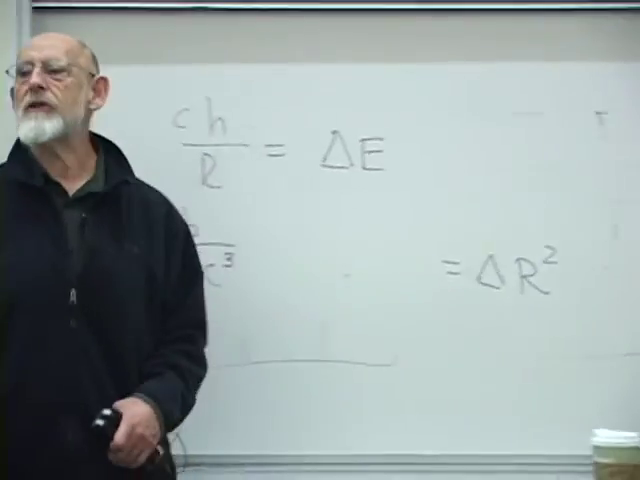
\includegraphics[width=0.84\textwidth]{lecture_02_figure_05.png}
\caption{黒板での完成したスケーリング議論。1ビットのエネルギー\(\Delta E\sim\hbar c/R_s\)は、\(G\hbar/c^3\)程度の半径の二乗、したがって面積の増分をもたらす。}
\lectureframe{01:22:40.000}
\end{figure}

実演計算の途中で\(c\)の因子が復元され、聴衆の一人がシュヴァルツシルト半径における欠落した\(c^{-2}\)を指摘する。その修正こそが式~\eqref{eq:planck-patch}における\(c^{-3}\)を生み出すものである。

\begin{classroomqa}
\audiencequestion{計算の一部だけで\(c\)を復元すると、その2乗を失うのか。\lecturetimestamp{01:21:18}}
\lecturerresponse{はい。次元関係は\(R_s=2GM/c^2\)であり、単に\(2GM\)ではない。その因子を復元すると面積は\(G\hbar/c^3\)のスケールになる。}
\end{classroomqa}

\(G\simeq6.7\times10^{-11}\,\mathrm{m^3\,kg^{-1}\,s^{-2}}\)、\(\hbar\simeq1.05\times10^{-34}\,\mathrm{J\,s}\)、\(c^3\simeq2.7\times10^{25}\,\mathrm{m^3\,s^{-3}}\)を用いると、
\begin{equation}
\ell_P^2\simeq2.6\times10^{-70}\,\mathrm{m^2},
\qquad
\ell_P\simeq1.6\times10^{-35}\,\mathrm{m}.
\end{equation}
黒板で見積もりを行う間、講義中の口頭の冪は揺れるが、物理的結論は安定している。このスケールは直接実験の分解能をはるかに下回る。

忘れがたいイメージは、鋭い肘をもつ不可侵のビットが地平線上に蓄積し、互いを押しのけ合うというものである。それぞれの新しいビットはおよそ1プランク面積のパッチを占める。これは面積の勘定のための比喩であって、文字どおりの正方形タイルが地平線を形成するという主張ではない。

\begin{classroomqa}
\audiencequestion{最初の光子がまだ近づいているときに、別の光子が地平線を拡大すると、古い光子は新しい地平線の内側に位置することになるのではないか。\lecturetimestamp{01:26:39}}
\lecturerresponse{単純な静的描像は、その問いを決着させるには十分に精密ではない。動的な時空における事象の地平線は大域的に定義されなければならず、その位置は物質が到着するにつれて変化する。ここで用いている外部記述では、情報は成長する地平線に関連づけられたままである。その地平線の厳密な定義は後回しにする。}
\end{classroomqa}

\begin{classroomqa}
\audiencequestion{巨大な質量が加えられる場合、たとえば二つのブラックホールが衝突する場合にも同じ問題が生じるのか。\lecturetimestamp{01:27:03}}
\lecturerresponse{はい。その場合には動的な性格を無視することは不可能である。講義では、地平線がより注意深く定義されるまで、合体の幾何学の完全な扱いを延期する。}
\end{classroomqa}

\begin{classroomqa}
\audiencequestion{プランク面積は、球面の地平線上ではなく、平らなパッチ上でのみ定義されるのか。\lecturetimestamp{01:27:30}}
\lecturerresponse{それは球面上の面積スケールであって、地平線が平らであることを要求するものではない。この数え上げにとって、平面か球面かという区別は重要ではない。}
\end{classroomqa}
\editorialnote{地平線の曲率半径が\(\ell_P\)に比べて巨大であるとき、各プランクサイズの近傍は局所的にほとんど平らである。}

直径八キロメートルの穴に対しては、限界の光子はそれに対応して、ほぼそのスケールの長い電波となる。聴衆向けの類推では、サイズに依存しない面積の増分を、バスケットボールの周りに巻いた紐にでも地球の周りに巻いた紐にでも同じ追加周長を加えることになぞらえている。どちらの場合も、固定された追加周長によって生じる半径方向の隙間は同じである。正確な幾何学は異なるが、どちらの例も、対象の元のサイズに依存しない変化を切り出している。

\section{面積の法則}

一度に1ビットずつ加えると、地平線の面積は普遍的な微視的量だけ変化する。したがって隠されうるビットの数は、体積ではなく\(A/\ell_P^2\)に比例しなければならない。ベッケンシュタインはこの比例関係を推論し、ホーキングの計算がその係数を確定した：
\begin{equation}
S_{\mathrm{BH}}=\frac{k_B A c^3}{4G\hbar}
=\frac{k_B A}{4\ell_P^2}.
\label{eq:bh-entropy}
\end{equation}
エントロピーを熱力学的単位ではなく二進ビットで数えるなら、\(S_{\mathrm{BH}}/k_B\)を\(\ln2\)で割る。

\begin{figure}[htbp]
\centering
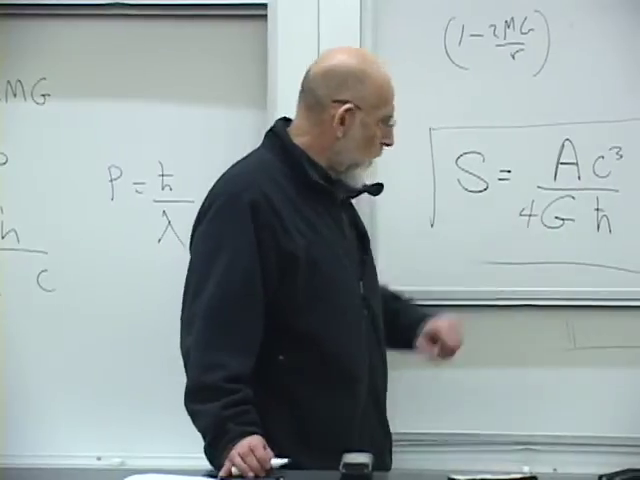
\includegraphics[width=0.84\textwidth]{lecture_02_figure_06.png}
\caption{ホーキングの因子\(1/4\)を含む最終的な板書の式は、講義のエントロピー単位で\(S\propto Ac^3/(4G\hbar)\)である。}
\lectureframe{01:31:02.000}
\end{figure}

したがってブラックホールは、同程度のサイズの通常の系よりも、桁違いに大きなエントロピーをもつ。それでもなお、その答えは素朴な体積の数え上げが示唆するよりも小さい。独立な情報は表面の測度によって制限される。この逆転---三次元の重力領域が二次元の境界としてスケールする情報によって記述されること---が、ホログラフィー原理の種である。

\begin{classroomqa}
\audiencequestion{エントロピーの式における因子\(1/4\)はどこから来るのか。\lecturetimestamp{01:30:30}}
\lecturerresponse{ベッケンシュタインの議論は面積への依存性と基本定数を確定したが、未知の係数を残した。彼の見積もりは2の対数などの可能性を生んだ。ホーキングの量子場の計算が係数を正確に\(1/4\)に確定した。}
\end{classroomqa}

\(\hbar\)の位置に最後の驚きが含まれている。量子エントロピーは\(\hbar\)に比例し、古典極限で消えると期待するかもしれない。そうではなく、\(\hbar\)が分母にある。\(\hbar\to0\)のとき、波は任意に小さいエネルギーコストで任意に細かい情報を運びうるので、エントロピー容量は発散する。量子化は、それ以外は古典的な穴に微小なエントロピーを加えるのではない。情報容量が無限になるのを防ぐのである。

\begin{classroomqa}
\audiencequestion{角運動量の単位をもつ\(\hbar\)が、通常の運動量と波長の関係も定めるのはなぜか。\lecturetimestamp{01:33:23}}
\lecturerresponse{\(\hbar\)は作用の単位、等価的には運動量×距離の単位をもつ。\(p\lambda\)が同じ単位をもつので、量子関係は\(2\pi\)の慣習を除いて\(p\sim\hbar/\lambda\)でありうる。角運動量\(\mathbf r\times\mathbf p\)が同じ次元をもつのは同じ理由による。}
\end{classroomqa}

講義はここで終わる。主題が尽きたからではなく、ここが正しい境界だからである。幾何学は地平線がなぜ情報を隠すのかを我々に告げ、熱力学は隠された情報をいかに数えるかを我々に告げ、量子力学はビット当たりの有限な面積を与えた。次の問いはもはや、ブラックホールが微視的状態を持つかどうかではなく、それらの状態が落下したものをどのように符号化し、最終的にどのように返すかである。
\chapter{平坦座標における地平線と蒸発の熱力学}

\lectureoverview{シュヴァルツシルト計量は地平線において特異になるように見えるが、自由落下する観測者はそこに何ら異常を感じないはずである。この緊張を、地平線近傍の計量を双曲極座標における平坦なミンコフスキー空間へ変換することによって解消する。同じ幾何学が、アリスの落下する記述とボブの加速された外部の記述とを分離する。後半ではエントロピーと温度を展開し、ホーキングの逆質量温度と\(M^3\)の蒸発則を導き、最後に情報の保存が重力の微視的理論に何を要求するかを問う。}

\section{\texorpdfstring{\(r=2GM\)}{r=2GM}における難問}

非常に大きなブラックホールから始めよう。その地平線は曲率が非常に小さいため、そこを落下して通過する観測者は、適度な実験室サイズの領域にわたって、ほとんど空の平坦な時空を見る。壁にぶつかることもなく、通過を告げる局所的な警報も鳴らない。それにもかかわらず、シュヴァルツシルト計量はまさにその半径において何か特異なことが起こると述べているように見える。講義の前半の目的は、これら二つの主張を両立させることである。

我々はmostly-plusの規約を用いる。平坦な時空では、
\begin{equation}
ds^2=-dt^2+dx^2+dy^2+dz^2,
\end{equation}
であるから、時間的worldlineは\(ds^2<0\)を持ち、固有時は\(d\tau^2=-ds^2\)を満たす。これは前の講義で用いた規約の全体的な符号反転である。観測可能な量はその選択に依存しない。

\(c=1\)とすると、シュヴァルツシルト線素は
\begin{equation}
\begin{aligned}
ds^2={}&-\left(1-\frac{2GM}{r}\right)dt^2
+\frac{dr^2}{1-\frac{2GM}{r}}
+r^2d\Omega_2^2,\\
d\Omega_2^2={}&d\theta^2+\sin^2\theta\,d\phi^2 .
\end{aligned}
\label{eq:l03-schwarzschild}
\end{equation}
である。シュヴァルツシルト半径は\(R_s=2GM\)、すなわち\(c\)を復元すれば\(R_s=2GM/c^2\)である。遠方では\(r\gg R_s\)であり、動径方向の両方の係数は平坦空間の値に近づく。しかし\(r=R_s\)では、\(dt^2\)の係数が消え、\(dr^2\)の係数が発散する。それは劇的に見える。問題は、幾何学が劇的なのか、それとも座標だけが劇的なのかである。

\section{二つの座標の教訓}

\subsection{極座標の無害な原点}

通常のユークリッド平面では、
\begin{equation}
ds^2=dx^2+dy^2.
\end{equation}
極座標を導入する。
\begin{equation}
x=\rho\cos\theta,
\qquad
y=\rho\sin\theta .
\end{equation}
微小変位は動径方向の長さ\(d\rho\)と横方向の長さ\(\rho\,d\theta\)を持つから、
\begin{equation}
ds^2=d\rho^2+\rho^2d\theta^2.
\label{eq:l03-polar}
\end{equation}
である。\(\rho=0\)では角度の係数が消える。これは平面の中心を特異にするものではない。そこでは\(\theta\)のどの値も同じ点を指すと述べているだけである。したがって、奇妙な計量の係数は、奇妙な物理ではなく奇妙な座標系を診断しているのかもしれない。

\subsection{双曲極座標}

次にユークリッド平面を\(1+1\)次元ミンコフスキー時空に置き換える。
\begin{equation}
ds^2=-dT^2+dX^2.
\end{equation}
右側のwedge\(X>|T|\)において、
\begin{equation}
X=\rho\cosh\omega,
\qquad
T=\rho\sinh\omega,
\qquad \rho>0 .
\label{eq:l03-rindler-transform}
\end{equation}
と定義する。通常の恒等式\(\cos^2\theta+\sin^2\theta=1\)は
\begin{equation}
\cosh^2\omega-\sinh^2\omega=1.
\end{equation}
に置き換えられる。したがって、\(\rho\)が一定の線は双曲線
\begin{equation}
X^2-T^2=\rho^2.
\end{equation}
である。周期的な角度\(\theta\)とは異なり、rapidity的な座標\(\omega\)は\(-\infty\)から\(+\infty\)まで走る。大きな正の\(\omega\)では、\(\cosh\omega\)と\(\sinh\omega\)はほとんど等しくなり、双曲線は未来のヌル光線\(X=T\)に近づく。

式~\eqref{eq:l03-rindler-transform}を微分すると
\begin{align}
dX&=\cosh\omega\,d\rho+\rho\sinh\omega\,d\omega,\\
dT&=\sinh\omega\,d\rho+\rho\cosh\omega\,d\omega .
\end{align}
が得られる。交差項は相殺され、
\begin{equation}
ds^2=-\rho^2d\omega^2+d\rho^2.
\label{eq:l03-rindler-metric}
\end{equation}
が残る。

\begin{figure}[htbp]
\centering
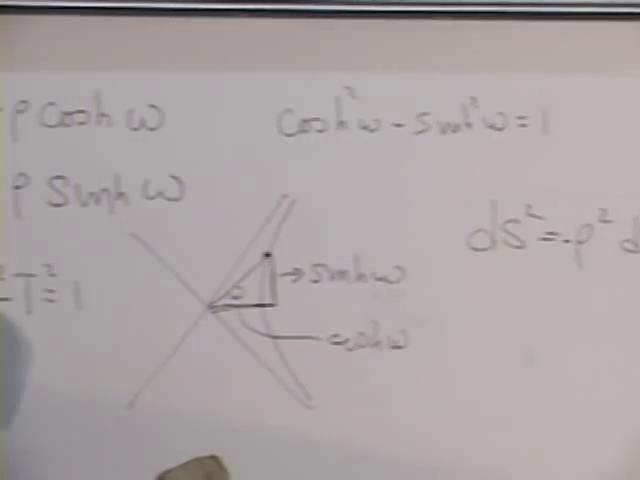
\includegraphics[width=0.72\textwidth]{lecture_03_figure_02.png}
\caption{完成した双曲座標の板書：\(X=\rho\cosh\omega\)、\(T=\rho\sinh\omega\)、単位双曲線の構成、そして\(ds^2=-\rho^2d\omega^2+d\rho^2\)の形の平坦計量。}
\lectureframe{00:16:55.000}
\end{figure}

式~\eqref{eq:l03-rindler-metric}は依然として完全に平坦な時空を記述している。その時間の係数は\(\rho=0\)で消える。ちょうど式~\eqref{eq:l03-polar}の角度の係数が原点で消えるのと同じである。そこでは座標チャートが退化するのであり、時空が退化するのではない。

\section{シュヴァルツシルト地平線へのズームイン}

式~\eqref{eq:l03-schwarzschild}の動径-時間部分に戻る。
\begin{align}
ds^2
&=-\frac{r-2GM}{r}\,dt^2
+\frac{r}{r-2GM}\,dr^2 .
\label{eq:l03-rewritten-schwarzschild}
\end{align}
ここで\(r=2GM\)の狭い近傍だけを調べる。ゆっくり変化する因子では、\(r\)を\(2GM\)で置き換えてよい。因子\(r-2GM\)は保持しなければならない。なぜならそれは地平線で消え、符号を変えるからである。したがって
\begin{equation}
ds^2\approx
-\frac{r-2GM}{2GM}\,dt^2
+\frac{2GM}{r-2GM}\,dr^2 .
\label{eq:l03-near-horizon-r}
\end{equation}

第二項が単に\(d\rho^2\)となるように新しい動径座標\(\rho\)を選ぶ。
\begin{equation}
d\rho^2=\frac{2GM}{r-2GM}\,dr^2.
\end{equation}
地平線の外側で、正の平方根をとり\(r=2GM\)から積分すると
\begin{align}
d\rho&=\sqrt{\frac{2GM}{r-2GM}}\,dr,\\
\rho&=2\sqrt{2GM}\sqrt{r-2GM},\\
\rho^2&=8GM(r-2GM),
\qquad
r-2GM=\frac{\rho^2}{8GM}.
\label{eq:l03-rho-r}
\end{align}
が得られる。式~\eqref{eq:l03-near-horizon-r}に代入すると
\begin{equation}
ds^2\approx
-\frac{\rho^2}{16G^2M^2}\,dt^2+d\rho^2.
\end{equation}
となる。最後にシュヴァルツシルト時間を再スケールし、
\begin{equation}
\omega=\frac{t}{4GM},
\qquad
d\omega^2=\frac{dt^2}{16G^2M^2},
\label{eq:l03-omega}
\end{equation}
を得る。
\begin{equation}
\boxed{ds^2\approx-\rho^2d\omega^2+d\rho^2.}
\label{eq:l03-near-horizon-rindler}
\end{equation}

\begin{figure}[htbp]
\centering
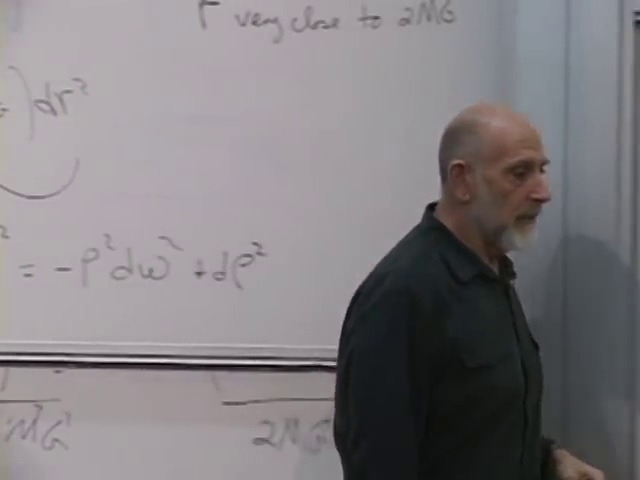
\includegraphics[width=0.70\textwidth]{lecture_03_figure_03.png}
\caption{時間再スケーリング後の板書：地平線近傍のシュヴァルツシルト計量は、平坦なミンコフスキー時空と同じ双曲極座標計量になった。}
\lectureframe{00:31:35.000}
\end{figure}

検査する近傍を地平線に向かって縮めていくと、この近似は際限なく良くなる。それは求められていた局所的な主張を証明している。すなわち、十分に大きな穴に対しては、地平線は異常な座標で書かれた通常の時空である。有限質量のシュヴァルツシルト穴に対して曲率が文字通りゼロであるわけではないが、地平線において有限であり、\(M\) を大きくすることでそこではいくらでも小さくできる。\editorialnote{局所的な曲率スケールは \(R_s^{-2}\) の程度である。リンドラー計量は地平線近傍の局所展開の主要項であり、シュヴァルツシルト幾何全体が大域的に平坦であるという主張ではない。}

\begin{classroomqa}
\audiencequestion{\(r<2GM\) に対して、式~\eqref{eq:l03-rho-r} はこの外部の \(\rho\) を虚数にする。これは物理的な問題を示しているのだろうか。\lecturetimestamp{00:32:30}}
\lecturerresponse{それは同じ座標の破綻を別の形で再現している。現在の座標は外部の楔のために構成されたものであり、地平線を越えて延長するには別の座標が必要である。この特定の \(\rho\) の破綻は、地平線における物理的な事象ではない。}
\end{classroomqa}

\begin{classroomqa}
\audiencequestion{地平線近傍への書き換えにおいて、近似された行は先行する厳密な行からどのように導かれるのか。\lecturetimestamp{00:39:21}}
\lecturerresponse{ゆっくりと変化する \(r\) の出現箇所だけが \(2GM\) に等しいと置かれている。小さな差 \(r-2GM\) はそのまま残されている。それがこの近似であり、\(r\) が \(2GM\) に近づくにつれてますます正確になる。}
\end{classroomqa}

\section{座標の意味}

この変換は次を同定する。
\begin{equation}
\rho=0\quad\Longleftrightarrow\quad r=2GM.
\end{equation}
外部 \(r>2GM\) は右リンドラー楔 \(X>|T|\) である。一定の \(\rho\) の双曲線は、固定されたシュヴァルツシルト半径にとどまる観測者を表す。その楔内のどこかで放出された外向きの光線は、より大きな \(\rho\) のすべての世界線と交差するので、外部の観測者は外向きに通信できる。未来のヌル境界を越えた点は、右の楔へ光信号を送り返すことができない。そのヌル境界が地平線である。

\begin{classroomqa}
\audiencequestion{ここに示された双曲線座標のパッチは、常に地平線の外側の領域を記述するのか。\lecturetimestamp{00:35:22}}
\lecturerresponse{はい。この構成では \(r>2GM\) が \(\rho^2>0\) を与え、事象を右の外部楔に置く。ヌル端 \(\rho=0\) が地平線であり、現在の座標はそれを越えて実の外部座標として続かない。}
\end{classroomqa}

\begin{classroomqa}
\audiencequestion{一定の \(\rho\) の双曲線は、一つの時間を表すのか、それとも一つの距離を表すのか。\lecturetimestamp{00:37:21}}
\lecturerresponse{それは地平線近傍近似において地平線からの一つの固定された固有距離を表し、したがって一つの固定されたシュヴァルツシルト半径を表す。双曲線に沿った運動は、そこに配置された観測者にとっての時間の経過である。}
\end{classroomqa}

固定された \(\rho\) の軌道に沿って、式~\eqref{eq:l03-rindler-metric} は次を与える。
\begin{equation}
d\tau=\rho\,d\omega.
\label{eq:l03-proper-time-rindler}
\end{equation}
したがって \(\omega\) はそれ自体では観測者の固有時ではない。それは双曲線の族に共通の角時間であり、各観測者はそれをその観測者の \(\rho\) で掛ける。ちょうど通常の角度が円の半径で掛けられて弧の長さを与えるのと同じである。

\begin{classroomqa}
\audiencequestion{\(\omega\) は加速する観測者の固有時か。\lecturetimestamp{00:51:45}}
\lecturerresponse{ほとんどそうである。固定された \(\rho\) において、固有時の増分は \(\rho\,d\omega\) である。\(\rho\) の因子が本質的である。}
\end{classroomqa}

\begin{figure}[htbp]
\centering
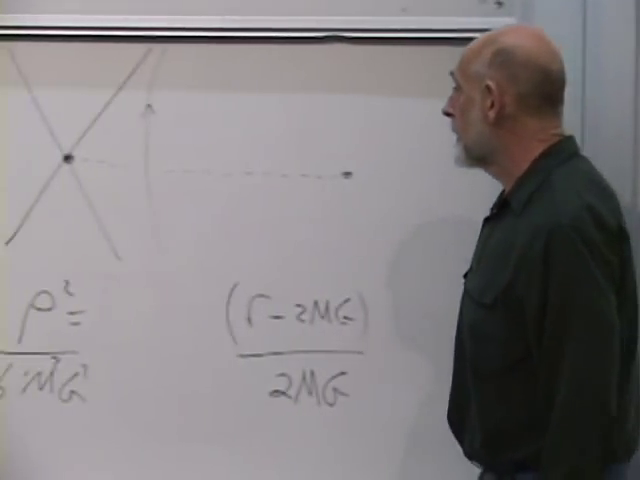
\includegraphics[width=0.72\textwidth]{lecture_03_figure_04.png}
\caption{地平線近傍の因果ボード。交差するヌル境界、外部楔における一定半径の双曲線、そして \(\rho\) と \(r-2GM\) の座標関係。}
\lectureframe{00:34:35.000}
\end{figure}

\begin{figure}[htbp]
\centering
\begin{tikzpicture}[scale=1.04,>=Latex]
  \draw[->] (-0.3,0) -- (4.6,0) node[right] {\(X\)};
  \draw[->] (0,-3.2) -- (0,3.2) node[above] {\(T\)};
  \draw[very thick,blue!55!black] (0,0) -- (3,3);
  \draw[very thick,blue!55!black] (0,0) -- (3,-3);
  \node[blue!55!black,rotate=45] at (0.72,1.02) {future horizon};
  \draw[thick,domain=-1.45:1.45,samples=80] plot ({0.75*cosh(\x)},{0.75*sinh(\x)});
  \draw[thick,domain=-1.25:1.25,samples=80] plot ({1.25*cosh(\x)},{1.25*sinh(\x)});
  \draw[very thick,domain=-1.05:1.05,samples=80] plot ({2.0*cosh(\x)},{2.0*sinh(\x)});
  \node at (3.64,2.18) {Bob: \(\rho=\mathrm{const.}\)};
  \draw[very thick,red!65!black,->] (1.2,-2.9) -- (1.2,2.9);
  \node[red!65!black] at (1.58,-1.75) {Alice};
  \fill[red!65!black] (1.2,1.2) circle (1.7pt);
  \draw[dashed,->] (1.2,0) -- (2.27,1.07);
  \node[align=left] at (3.18,0.80) {\small pre-crossing\\[-0.2em]\small light signal};
\end{tikzpicture}
\caption{ボードの組版された相棒。ボブは加速された一定の \(\rho\) の双曲線に従い、アリスは未来の地平線を通る局所的に慣性の直線に従う。ヌル境界は、アリスにとって局所的な障害となることなく、ボブの因果的アクセスを制限する。}
\end{figure}

\section{アリスは落下し、ボブはホバリングする}

ボブが地平線から固定された距離を保つ一方で、アリスは彼の手を離して落下する。ボブの世界線は双曲線であり、したがって加速されている。アリスの局所的な世界線はほぼ直線である。彼女は有限の固有時間でヌル境界を横切り、局所的な不連続に遭遇しない。

因果的記述は非対称である。アリスが横切った後、彼女からの光はボブに届かないが、ボブが放った光はしばらくの間アリスに届く。ボブは、アリスの有限な落下の次第に早い段階で放たれた信号を受け取る。それらの到達時刻はますます引き離され、周波数は赤方偏移し、強度は弱まる。シュヴァルツシルト時間では、彼は横断そのものを決して見ない。アリスは地平線に漸近的に近づき、それに張り付いて平坦化するように見える。彼女の鼻が平坦化する一方で後頭部が普通のままである、というのではない。あらゆる部分からの信号が同じ極限的な層に圧縮されるのである。

\begin{classroomqa}
\audiencequestion{アリスは横切った後、ボブの光子が彼女に向かって内向きに進むのでボブを見ることができるのか。\lecturetimestamp{00:42:48}}
\lecturerresponse{はい。一方向の因果関係が要点である。ボブの内向きの信号は入ることができるが、アリスの後の外向きの信号はボブへ逃げ戻ることができない。}
\end{classroomqa}

\begin{classroomqa}
\audiencequestion{アリスの足が先に横切り、目が外側に残っているなら、彼女は一時的に自分の足を見失うのか。\lecturetimestamp{00:43:03}}
\lecturerresponse{通常の落下では視覚的な途切れはない。光は足から目まで進むのに常に時間がかかる。関連する信号が到着するころには、彼女の目も横切っている。足が内向きに進み続ける間、頭を外側に保持しようとする激しい試みだけが、異なる破壊的な状況を生むであろう。}
\end{classroomqa}

位置を保持することは非慣性の選択である。ボブにはロケットが必要である。ちょうど床に立っている人には自由落下を避けるために床の上向きの力が必要であるのと同じである。ボブが地平線に近くホバリングするほど、必要な固有加速度は大きくなる。局所リンドラー近似では、その大きさは単位\(c=1\)で\(a=1/\rho\)である。\editorialnote{単位を戻すと、局所リンドラー観測者に対して\(a=c^2/\rho\)となる。厳密に静的シュヴァルツシルト観測者の固有加速度は、地平線に近づくにつれて発散する。}

\begin{classroomqa}
\audiencequestion{講義室に立っているとき、我々は加速しているのか。\lecturetimestamp{00:45:40}}
\lecturerresponse{はい、自由落下系に対してである。床が我々を支えている。床がなければ、あるいはジェットパックがなければ、我々は落下するであろう。}
\end{classroomqa}

\begin{classroomqa}
\audiencequestion{ボブは最終的に、地平線から1プランク長以内にいるアリスを見るのか。そしてその後何が起こるのか。\lecturetimestamp{00:49:24}}
\lecturerresponse{そこでは古典的幾何学的記述が十分でなくなる。プランク長には\(\hbar\)が含まれるので、そこでボブが何を分解できるかを答えるには量子力学が必要である。}
\end{classroomqa}

\begin{classroomqa}
\audiencequestion{一定半径の曲線は、直角のような座標の角で地平線に出会うように見える。そこで微分を取ることができるのか。\lecturetimestamp{00:51:12}}
\lecturerresponse{その点でこの座標チャートに特異なことが起こるが、局所物理には起こらない。他の楔を覆うチャートは人為的な角を取り除く。現在の外部に関する議論では、リンドラー描像が必要な因果的事実をすでに含んでいる。}
\end{classroomqa}

したがって、観測者を指定せずに、アリスが\emph{本当に}横切るのかどうかを問うことは役に立たない。アリスの時計は有限の固有時間で地平線に達する。ボブが受け取る信号列には横断事象が決して含まれない。物理学は、各観測者が何を測定し、それらの記録をどのように比較できるかを問う。

\begin{classroomqa}
\audiencequestion{ボブ自身の観測時間は非有界であるにもかかわらず、ボブはアリスの未来の有限部分しか見ることができない、というのが鋭い主張か。\lecturetimestamp{00:53:33}}
\lecturerresponse{はい。アリスは自分の落下の可視部分に有限の固有時間を割り当てる。理想化された永遠の幾何学では、ボブはますます遅延し赤方偏移したその信号を永遠に受け取るが、地平線横断を超えて彼女が年を取り続けるのを見ることはない。}
\end{classroomqa}

\section{加速地平線だけで十分である}

この因果構造にはブラックホールを必要とするものは何もない。永遠に一様に加速し続けるロケットは、平坦時空内でリンドラー双曲線に沿って進み、信号がそれに追いつけない零境界を持つ。その観測者にとって加速地平線が存在する。慣性観測者は同じ領域を通常のミンコフスキー空間とみなすにもかかわらず、である。

\begin{classroomqa}
\audiencequestion{この現象はブラックホールに固有のものか、それとも任意の地平線で起こるのか。\lecturetimestamp{00:55:25}}
\lecturerresponse{同じ現象は一様に加速する観測者でも起こる。そのような観測者には加速地平線があり、その先の事象を見ることはできない。局所的には、ブラックホールの地平線はその場合と物理的に異ならない。}
\end{classroomqa}

これは等価原理が働いている例である。まず一様加速を理解し、次に重力場の中に同じ局所構造を見出すのである。振り返れば、ブラックホールが受け入れられる以前から、加速の地平線から重力の地平線を予期できたはずである。アインシュタイン自身は、ブラックホールの物理的形成を受け入れなかった。その幾何学が従う理論を与えたにもかかわらず、である。地平線は自由落下する観測者にとっては退屈であり、外にとどまることに固執する観測者にとっては重大な帰結をもつ。これは有効な記述の間の緊張であって、まだパラドックスではない。

\section{熱とエントロピーに戻る}

休憩の後は、熱力学の帽子をかぶろう。前の構成では、ブラックホールは浴槽のように一滴ずつ満たされた。ただし、各滴はおよそ1ビットを運ぶ光子であった。各ビットは地平線の面積をプランク面積程度の量だけ増加させた。正確なエントロピーは
\begin{equation}
S_{\mathrm{BH}}=\frac{k_B A}{4\ell_P^2}.
\end{equation}
講義では、プランクが自分の長さを別様に定義していれば因子\(1/4\)は避けられたはずだと冗談を言う。真剣な点は、次元解析はスケールを固定するが数値係数は固定しないということである。ホーキングの計算がその係数を固定する。\editorialnote{プランク長には標準的な定義\(\ell_P=\sqrt{G\hbar/c^3}\)がある。この慣習と通常の熱力学的エントロピーを固定すれば、因子\(1/4\)は物理的である。これを再定義するという発言は、慣習についての教室での冗談である。}

温度は、指や温度計が直接それを感知するため、初等的に感じられる。エントロピーはしばしばより神秘的に感じられる。この講義はその階層を逆転させる。すなわち、エントロピーとエネルギーを基本的な変数として扱い、温度はエントロピーが変化するときにエネルギーがどれだけ変化しなければならないかから導かれる：
\begin{equation}
dE=T\,dS.
\end{equation}
講義の1ビット単位では\(\Delta S=1\)であるため、ビットを追加または消去する際に伴う最小エネルギーは\(T\)と呼ばれる。注意深さを欠いて---論理的に言えば大ハンマーに相当するもので---消去すると、任意にそれ以上のエネルギーを散逸させうる。この定義は、失われた情報が微視的な環境自由度へ移される際に可能な最小の散逸に関するものである。従来の単位では、1つの二進ビットは\(\Delta S=k_B\ln2\)を担い、可逆的な消去は少なくとも\(k_BT\ln2\)を散逸させる。\editorialnote{これは、講義がエントロピーと温度の両方をエネルギーに基づく自然単位で測ることを選んだために抑制されているランダウアーの規格化である。}

\subsection{1光子の見積もり}

波長がシュヴァルツシルト半径と同程度の光子を選ぶ：
\begin{equation}
\lambda\sim R_s=\frac{2GM}{c^2}.
\end{equation}
そのエネルギーは、\(h\)と\(\hbar\)を区別する\(2\pi\)の慣習を除いて、
\begin{equation}
\Delta E\sim \frac{\hbar c}{\lambda}.
\end{equation}
これが加えられたビットのエネルギーコストなので、
\begin{equation}
k_BT_H\sim\frac{\hbar c}{R_s}
\sim\frac{\hbar c^3}{GM}.
\label{eq:l03-hawking-scale}
\end{equation}
この発見的議論では\(2\)や\(\pi\)のような因子は決定できない。正確なホーキングの結果は
\begin{equation}
\boxed{k_BT_H=\frac{\hbar c^3}{8\pi GM}.}
\label{eq:l03-hawking-exact}
\end{equation}

\begin{figure}[htbp]
\centering
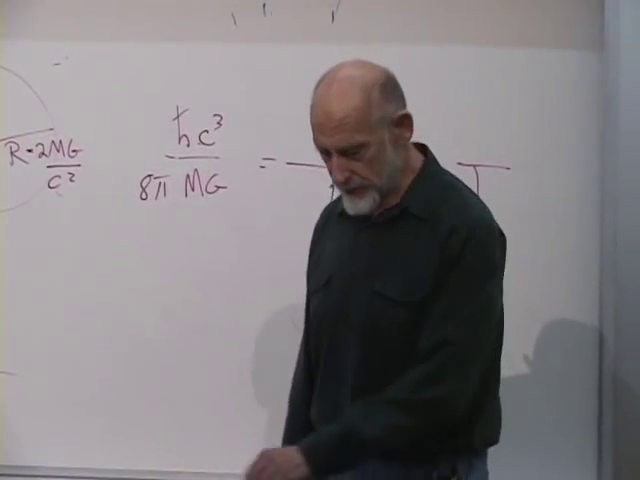
\includegraphics[width=0.72\textwidth]{lecture_03_figure_05.png}
\caption{完成した温度の板書：\(R_s=2GM/c^2\)、1ビットのスケール\(\hbar c/R_s\)、そして正確な\(8\pi\)のホーキング規格化。}
\lectureframe{01:07:48.000}
\end{figure}

ただちに二つの事実が導かれる。第一に、温度は\(\hbar\)とともに消えるので、これは量子効果である。第二に、
\begin{equation}
T_H\propto\frac{1}{M}.
\end{equation}
大きなブラックホールは冷たい。太陽質量1つに対して、
\begin{equation}
T_H\approx6\times10^{-8}\ {\rm K},
\end{equation}
これは講義の\(10^{-8}\,\mathrm{K}\)という見積もりと同じ程度の桁であり、宇宙マイクロ波背景放射の温度約\(2.7\,\mathrm{K}\)よりはるかに低い。

\subsection{負の熱容量}

そのようなブラックホールをより暖かい環境に置く。それはエネルギーを吸収し、質量が増加し、式~\eqref{eq:l03-hawking-exact}によればより冷たくなる。するとさらに吸収しやすくなる。より冷たい環境に置けば逆の暴走が始まる。それは放射し、質量を失い、より熱くなり、より速く放射する。形式的には、
\begin{equation}
C_{\mathrm{BH}}
=\frac{dE}{dT_H}
=c^2\frac{dM}{dT_H}
<0.
\end{equation}

\begin{classroomqa}
\audiencequestion{これが負の比熱という意味ですか。\lecturetimestamp{01:14:08}}
\lecturerresponse{まさにそのとおり。自己重力系はエネルギーを失いながら熱くなりうる。恒星も類似のことをする。放射すると圧力が下がって収縮し、重力圧縮がその温度を上げる。}
\end{classroomqa}

孤立したブラックホールがそれゆえ非物理的になるわけではない。今日の宇宙では、恒星質量のブラックホールは周囲より冷たく、主に吸収する。宇宙が膨張し背景が冷えるにつれ、バランスはやがて逆転し、蒸発が支配的になりうる。実効的に無限の熱浴との単純な平衡は不安定である。\editorialnote{境界条件が重要である。ブラックホールは有限の反射空洞の中や、適切な大きなブラックホールに対しては反ド・ジッター時空の中で安定化されうる。ここで述べた不安定性は、漸近的に平坦な通常の熱浴の場合である。}

\section{蒸発則}

スケーリングの導出にあたっては、参考書がない状況を想像し、記憶している方程式が最も短くなる単位を選ぶ：
\begin{equation}
c=\hbar=G=k_B=1.
\end{equation}
これらはプランク単位である。講義で引用された特徴的なスケールは
\begin{equation}
\ell_P\sim10^{-35}\ {\rm m},
\qquad
t_P\sim10^{-43}\ {\rm s},
\qquad
m_P\sim10^{-8}\ {\rm kg}.
\end{equation}
プランク質量はおおよそ目に見える塵の粒ほどであるが、プランク長とプランク時間は極めて小さい。\(c=1\) であるから、\(t_P\) は単に \(\ell_P\) を光が横切る時間である。

穴を黒体として扱う。すなわち、完全に暗いままでなければならない物体ではなく、熱的な放射体とみなす。それは電磁放射を放出でき、原理的にはグラビトンを含む他の利用可能な種も放出しうる。放射は表面を通って出ていくので、放射されるパワーは放射面積に比例する。シュテファン--ボルツマンのスケーリングは
\begin{equation}
L=-\frac{dE}{dt}\sim A T^4.
\end{equation}
プランク単位では \(E=M\)、\(R_s\sim M\)、\(A\sim R_s^2\sim M^2\)、\(T\sim R_s^{-1}\sim M^{-1}\) である。したがって
\begin{align}
-\frac{dM}{dt}
&\sim R_s^2\left(\frac{1}{R_s}\right)^4
\sim\frac{1}{R_s^2}
\sim\frac{1}{M^2},\\
-M^2\frac{dM}{dt}&\sim1,\\
-\frac{d(M^3)}{dt}&\sim1.
\label{eq:l03-evap-scaling}
\end{align}
1次の係数を無視すると、寿命は
\begin{equation}
\boxed{t_{\mathrm{evap}}\sim M^3.}
\label{eq:l03-lifetime}
\end{equation}

\begin{figure}[htbp]
\centering
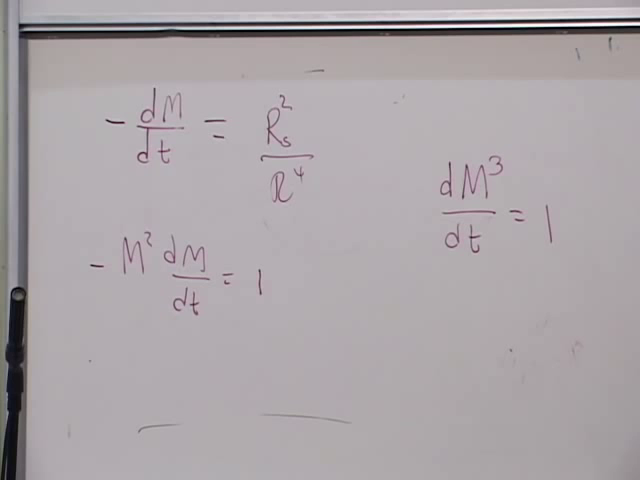
\includegraphics[width=0.72\textwidth]{lecture_03_figure_06.png}
\caption{妨げのない蒸発盤：光度は\(-dM/dt\sim1/M^2\)を与え、したがって\(M^3\)の一様な減少と、初期質量の三乗に比例する寿命が得られる。}
\lectureframe{01:23:20.000}
\end{figure}

この模式的なシュテファン--ボルツマン的取り扱いは、グレイボディ因子と粒子種の数を抑圧している。中性で回転しない穴について、最も単純な無質量放出近似で定数を復元すると
\begin{equation}
t_{\mathrm{evap}}
=\frac{5120\pi G^2M_0^3}{\hbar c^4}.
\label{eq:l03-exact-lifetime}
\end{equation}
この係数は編集上の補完であり、講義は頑健な \(M_0^3\) 依存性のみを導出している。

\subsection{太陽、山、キログラムのスケール}

太陽の質量は\(M_\odot\sim10^{30}\,\mathrm{kg}\sim10^{38}m_P\)である。これを三乗し、一プランク時間を掛けると、講義の意図的に粗い連鎖
\begin{equation}
t_{\mathrm{evap}}\sim10^{114}t_P
\sim10^{71}\ {\rm s}
\sim10^{64}\ {\rm yr}.
\end{equation}
が得られる。どちらの推定値も、宇宙のおよそ\(10^{10}\)年の年齢より途方もなく長い。式~\eqref{eq:l03-exact-lifetime}の係数を復元すると、標準的な太陽質量の推定値は約\(2\times10^{67}\)年になる。\editorialnote{この違いは予想されるものである。黒板での計算はすべての数値定数を落とし、プランクスケールを十の冪で丸めている。その目的は質量の三乗スケーリングであり、精密な寿命天文学ではない。}

次にクラスは\emph{山の質量}の穴を試す。教室での粗い値\(M\sim10^{10}\,\mathrm{kg}\)、したがって\(M\sim10^{18}m_P\)に落ち着き、
\begin{equation}
t_{\mathrm{evap}}\sim10^{54}t_P
\sim10^{11}\ {\rm s}
\sim10^4\ {\rm yr}.
\end{equation}
を得る。これは黒板で実際に行われた算術を保持している。その質量を動機づけるために用いられた言葉による幾何学---およそ\(100\,\mathrm{km}^3\)の岩石---は、実際にははるかに重く、正確な寿命の係数も結果を大きく変えるであろう。\editorialnote{通常の岩石密度では、\(100\,\mathrm{km}^3\)は\(10^{14}\,\mathrm{kg}\)の程度であり、\(10^{10}\,\mathrm{kg}\)ではない。\(10^{10}\,\mathrm{kg}\)に対して、式~\eqref{eq:l03-exact-lifetime}は\(10^6\)年の程度の寿命を与える。これらの補正は、寿命が質量の三乗として減少するという講義の教訓を変えない。}

\begin{classroomqa}
\audiencequestion{質量がわずか一キログラムのブラックホールは極端に小さいだろうか？\lecturetimestamp{01:29:14}}
\lecturerresponse{はい。半径は質量に比例し、太陽質量は数キロメートルに対応するので、一キログラムのシュヴァルツシルト半径は約\(10^{-27}\,\mathrm{m}\)である。そのような穴はまた極端に高温で短命であろう。}
\end{classroomqa}

\begin{classroomqa}
\audiencequestion{これらの蒸発の推定は周囲温度がゼロであると仮定しているのか？\lecturetimestamp{01:29:53}}
\lecturerresponse{それらは周囲が穴より冷たく、正味のエネルギーが外へ流れる場合に適用される。より高温の環境は代わりにブラックホールにエネルギーを供給する。ホーキング温度が現在の背景放射と一致する質量は演習問題として残されている。}
\end{classroomqa}

目安として、\(T_H=2.7\,\mathrm{K}\) と置くと \(M\) は \(10^{22}\,\mathrm{kg}\) の程度となり、シュヴァルツシルト半径は \(10^{-4}\,\mathrm{m}\) の程度となる。\editorialnote{これは講義で出された演習問題を評価するものであり、話された導出の一部ではない。}

\section{計量の下には何がなければならないか？}

\begin{classroomqa}
\audiencequestion{どのような機構が光子をブラックホールから出させるのか？\lecturetimestamp{01:30:53}}
\lecturerresponse{放射の微視的機構を与える前に、エントロピーの原因となる自由度を同定しなければならない。熱力学的議論は、それらの変数をまだ明示的に示すことなく、何が存在しなければならないかを制約する。}
\end{classroomqa}

類推は流体力学である。流体力学は、すべての分子を追跡することなく、滑らかな密度場と速度場を記述する。それにもかかわらず、エントロピーは、同じ滑らかな状態の背後に多くの隠れた微視的配置があることを明らかにする。同様に、古典的一般相対論は滑らかな計量を記述するが、ブラックホールエントロピーによって数えられる多数の微視的自由度を露わにしない。面積則とホーキング放射は、アインシュタインの理論が有効な巨視的記述であることの手がかりである。

\begin{classroomqa}
\audiencequestion{ブラックホールがエネルギーを放射するなら、それは情報を放射すると言うのと同じことで、成長中に飲み込まれた情報が蒸発中に戻ってくるのだろうか？\lecturetimestamp{01:33:27}}
\lecturerresponse{それが要請である。完全な時間発展が情報を保存するなら、出ていく放射は最終的に、ブラックホールを形成した可能な状態を区別できなければならない。これは依然として、物質が事象の地平面を横切るという因果的な描像と折り合いをつけなければならない。}
\end{classroomqa}

エネルギーの流れだけでは情報を指定するのに十分ではない。完全に熱的な密度行列は、詳細な初期状態を忘れつつエネルギーを運ぶことができる。ユニタリーな記述では、必要な情報は放出された量子間の微細な相関に符号化されている。\editorialnote{この区別は情報問題の現代的な形を明示する。それは講義で提起された問いを鋭くするのであって、変えるのではない。}

\section{情報保存の構造的原理としての位置づけ}

\begin{classroomqa}
\audiencequestion{情報の保存は本当に基本原理なのだろうか？\lecturetimestamp{01:34:13}}
\lecturerresponse{それは最も基本原理的なものの一つである。異なる初期状態がまったく同じ最終状態へと発展しうるなら、法則は自らの過去を消去してしまうことになる。通常の保存則は対称性だけでなく、可逆なハミルトニアン、すなわちユニタリーな形の時間発展にも依拠している。}
\end{classroomqa}

講義がそうするように、滑っている消しゴムをすべて単に静止させる架空の基本法則を想像してみよ。異なる初速度がすべて同じ状態に終わる。最終状態の消しゴムはもはやその履歴を区別しない。情報は破壊されている。運動量と力学的エネルギーも消える。現実の摩擦は微視的レベルではこうはならない。運動量とエネルギーは机、空気、熱的自由度へと移る。

完全に一様な無限の卓上であっても並進対称性をもつが、それでも架空の減衰法則は消しゴムを停止させうる。したがって並進対称性だけでは、そのような非ハミルトニアン的規則から運動量保存を導くのに十分ではない。ネーターの定理は作用原理とそれに伴う可逆な力学を前提とする。ここで用いられている言葉では、対称性と情報保存的な力学が保存則を与える。

\begin{classroomqa}
\audiencequestion{情報保存は因果性よりも基本原理なのだろうか？\lecturetimestamp{01:37:00}}
\lecturerresponse{それらは同程度に基礎的なレベルにある異なる原理である。因果性はまず正確に述べられなければならない---たとえば、信号は許された因果構造の外へ逆向きに伝播できないということ---が、どちらの原理も単純に他方を置き換えることはできない。}
\end{classroomqa}

\begin{classroomqa}
\audiencequestion{ハミルトン力学で議論される位相空間の面積保存は、この考えの古典版なのだろうか？\lecturetimestamp{01:37:38}}
\lecturerresponse{そのとおりである。リウヴィルの定理は、ハミルトン流が位相空間の体積を保存すると述べている。可能な初期状態の雲は、より小さな体積へと崩壊して区別を消去することはできない。量子力学では対応する主張はユニタリー性である。内積、したがって直交状態間の区別が保存される。}
\end{classroomqa}

古典的には、
\begin{equation}
\frac{d}{dt}\,\mathrm{Vol}_{\Gamma}=0,
\end{equation}
ハミルトン流によって輸送される位相空間領域に対して成り立つ。量子力学的には、
\begin{equation}
\begin{aligned}
\ket{\psi(t)}&=U(t)\ket{\psi(0)},\\
U^\dagger U&=I,\\
\braket{\psi(t)}{\phi(t)}
&=\braket{\psi(0)}{\phi(0)}.
\end{aligned}
\end{equation}
これらは、微視的な区別が時間発展を通じて生き残るという主張の正確な形である。

\section{エントロピーはどちらに依存するのか？}

最後のやり取りは情報理論的エントロピーに戻る。微視的な選択肢に対する確率\(p_i\)が与えられたとき、
\begin{equation}
S=-k_B\sum_i p_i\ln p_i
\label{eq:l03-shannon}
\end{equation}
熱力学的単位では、あるいは\(k_B\)を付けずに無次元のシャノンエントロピーとして表される。

\begin{figure}[htbp]
\centering
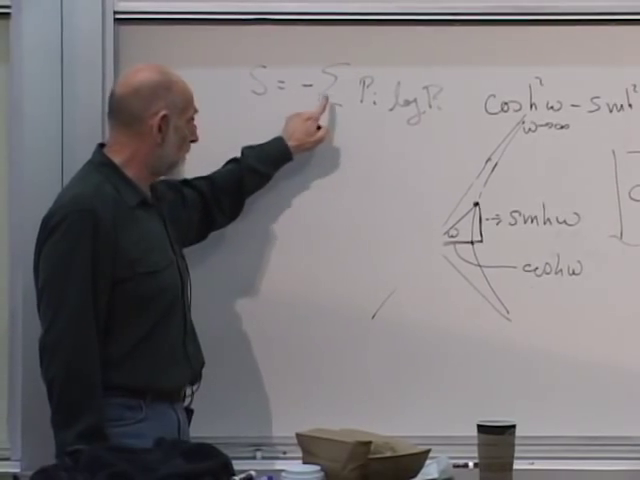
\includegraphics[width=0.72\textwidth]{lecture_03_figure_07.png}
\caption{最後の板書の式\(S=-\sum_i p_i\log p_i\)は、確率分布とそれから計算される単一のエントロピー値を区別しながら書かれたものである。}
\lectureframe{01:40:32.000}
\end{figure}

\begin{classroomqa}
\audiencequestion{エントロピーを最大化することが確率分布を定義するのであって、確率がエントロピーを定義するのではないのか？\lecturetimestamp{01:38:33}}
\lecturerresponse{確率分布は式~\eqref{eq:l03-shannon}を通じて一つのエントロピー値を定める。一つの数からすべての\(p_i\)を再構成することはできない。エントロピーの最大化が分布を選び出せるのは、規格化や、固定された平均エネルギーなどの他の制約も与えられた後だけである。}
\end{classroomqa}

この区別が講義をまさに正しい最前線で終わらせる。滑らかな幾何学は地平面へと導いた。地平面は熱力学へと導いた。熱力学は隠れた自由度を露わにした。そして情報保存は今や、それらの自由度が、ブラックホールに入った区別を消去することなく発展することを要求している。その機構はまだ与えられていない。代わりに幾何学と帳簿付けが、成功するどんな微視的理論も説明しなければならないことを明らかにしたのである。

\chapter{ブラックホール、ホワイトホール、大域的因果図}

\lectureoverview{事象の地平面は局所的には何ら特別なものではなく、大域的には決定的な意味をもつ。まず地平線近傍のシュヴァルツシルト計量から出発し、ユークリッドの葉巻の類推を用いてそれを外側へとたどり、次にアリスとボブが実際に何を見ることができるかを問う。特異点と時間反転されたホワイトホール領域は、その局所的描像を永遠のシュヴァルツシルト時空へと拡大する。ペンローズのコンパクト化により、因果構造は有限で読み取れるものになる。最後の段階では、永遠の解から、重力崩壊によって作られたブラックホールへと移る。そこではニュートンの球殻定理とバーコフの定理が、接合すべき部品を与える。}

\section{地平線から無限遠まで}

十分に大きなシュヴァルツシルト地平線の近傍では、小さな実験室の範囲で曲率は弱く、動径-時間幾何は近似的に平坦である。便利な動径変数はシュヴァルツシルト座標\(r\)ではなく、一定時刻の空間的断面に沿って地平線から外向きに測った固有距離\(\rho\)である：
\begin{equation}
\rho=0 \quad\Longleftrightarrow\quad r=2GM .
\label{eq:l04-rho-horizon}
\end{equation}
便利な時間座標は無次元量
\begin{equation}
\omega=\frac{t}{4GM},
\label{eq:l04-omega}
\end{equation}
である。ここで\(c=1\)である。したがって\(\omega\)は、シュヴァルツシルト半径の2倍を単位として測ったシュヴァルツシルト時間である。

mostly-plusの規約では、地平線近傍の動径-時間計量は
\begin{equation}
ds^2\approx-\rho^2d\omega^2+d\rho^2.
\label{eq:l04-rindler}
\end{equation}
である。角方向の2次元球面は省略した。現在の議論は時間と動径距離のみに関わるからである。

\begin{figure}[htbp]
\centering
\includegraphics[width=0.72\textwidth]{lecture_04_figure_02.png}
\caption{地平線近傍の計量と再スケールされたシュヴァルツシルト時間。}
\lectureframe{00:05:46.800}
\end{figure}

式~\eqref{eq:l04-rindler}は、極座標がユークリッド平面に対して持つ関係と同じ関係をミンコフスキー時空に対して持つ。
\begin{equation}
T=\rho\sinh\omega,
\qquad
X=\rho\cosh\omega,
\end{equation}
に対して
\begin{equation}
-dT^2+dX^2=-\rho^2d\omega^2+d\rho^2.
\end{equation}
が得られる。\(\rho\)が一定の線は双曲線\(X^2-T^2=\rho^2\)であり、一方\(\omega\)は遠い過去から遠い未来へと走る。2本のヌル線\(X=\pm T\)は、縮約された図の分岐点で交わる。4次元ではその点は2次元球面を表し、未来と過去のヌル面は分岐キリング地平線を形成する。\editorialnote{交差点のみを分岐地平線と呼ぶのは、動径図における有用な略記法である。より正確には、2つの地平線の枝は分岐2次元球面上で交わる。}

\subsection{遠方領域}

シュヴァルツシルト計量の動径-時間部分は
\begin{equation}
ds^2
=-\left(1-\frac{2GM}{r}\right)dt^2
+\frac{dr^2}{1-\frac{2GM}{r}}.
\label{eq:l04-schwarzschild}
\end{equation}
である。ブラックホールから遠く、\(r\gg2GM\)では、計量は
\begin{equation}
ds^2\approx-dt^2+dr^2.
\end{equation}
に近づく。そこでは\(r\)と\(\rho\)は本質的でない加法的補正だけ異なるので、\(dt=4GM\,d\omega\)とすると、
\begin{equation}
ds^2\approx-(4GM)^2d\omega^2+d\rho^2.
\label{eq:l04-far}
\end{equation}
となる。動径方向の係数は両方の極限で単純である。変化するのは時間方向の係数である：
\begin{equation}
ds^2\approx
\begin{cases}
-\rho^2d\omega^2+d\rho^2, & \rho\ll GM,\\[3pt]
-(4GM)^2d\omega^2+d\rho^2, & \rho\gg GM.
\end{cases}
\label{eq:l04-two-limits}
\end{equation}
ホバリングする軌道に沿っては、\(d\rho=0\)である。地平線の近くでは、
\begin{equation}
d\tau=\rho\,d\omega,
\end{equation}
であるのに対し、遠方では\(d\tau\approx4GM\,d\omega=dt\)である。外部時間座標の一定の増分に対して、地平線により近く保持された時計では、経過する固有時間はますます少なくなる。

\subsection{葉巻}

時空は描きにくいので、時間的方向を通常の角度方向で置き換える。
\begin{equation}
\begin{aligned}
d\ell^2&=F(\rho)^2d\theta^2+d\rho^2,\\
F(\rho)&\sim
\begin{cases}
\rho, & \rho\to0,\\
4GM, & \rho\to\infty.
\end{cases}
\end{aligned}
\label{eq:l04-cigar}
\end{equation}
と書く。\(\rho=0\)の近くでは、これは極座標における平面である。遠方では、円周はもはや半径とともに増大しない：
\begin{equation}
C_\infty=\int_0^{2\pi}4GM\,d\theta=8\pi GM.
\label{eq:l04-cigar-circumference}
\end{equation}
したがってこの曲面は一方の端で丸みを帯び、他方の端で円柱に近づく。それは葉巻のように見える。

\begin{figure}[htbp]
\centering
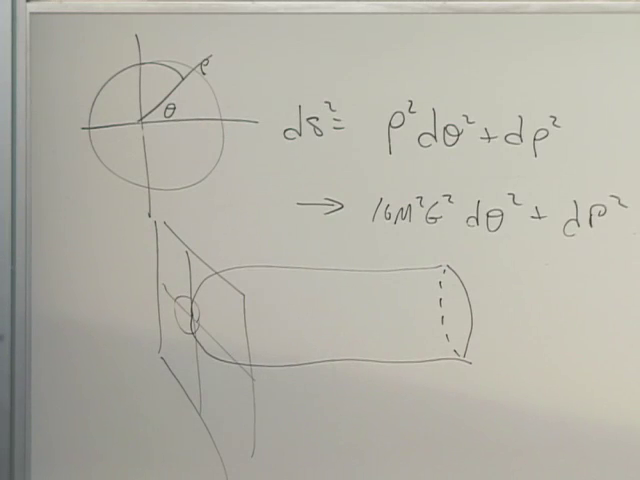
\includegraphics[width=0.74\textwidth]{lecture_04_figure_03.png}
\caption{ユークリッド的比較：極の先端が、周長\(8\pi GM\)の漸近的円柱に接合されている。}
\lectureframe{00:14:05.000}
\end{figure}

質量が大きいほど、漸近的な太さは大きくなり、先端近くの曲がりは緩やかになる。小さな穴は強く曲がった葉巻に対応し、大きな穴は広く弱く曲がった先端をもつ。これは式~\eqref{eq:l04-two-limits}における補間の描像であり、ローレンツ的ブラックホールそのものの埋め込みではない。\editorialnote{正確な幾何学的対象は、シュヴァルツシルト時間を虚時間へ解析接続することによって得られる。そのとき先端での滑らかさがユークリッド時間の周期を\(8\pi GM\)に固定する。これは後にホーキング温度を決定するのと同じスケールである。ここでは講義は視覚的類推のみを用いている。}

\section{地平線を因果的に読む}

穴の外側、\(\rho>0\)では、静止観測者は\(\rho\)が一定の双曲線に沿う。遠方では、重力に抗するのに必要な加速度はわずかである。地平線の近くでは、必要な固有加速度は際限なく増大する。世界線が未来のヌル境界を一度横切ると、そこからの未来向きの因果的信号は外部に到達できない。

\begin{classroomqa}
\audiencequestion{この図で光線は直線か？\lecturetimestamp{00:20:21}}
\lecturerresponse{別の規約が述べられない限り、動径方向の光線は\(45^\circ\)に描かれる。内向きの光線は地平線を横切る。すでに内部にある外向きの光線は、外部へと逆に横切ることはできない。}
\end{classroomqa}

\begin{classroomqa}
\audiencequestion{入射光線は地平線上にとどまるか。\lecturetimestamp{00:21:12}}
\lecturerresponse{いいえ。内向きに放たれた光線は未来の地平線を横切り、ブラックホール内部へと進み続ける。地平線の生成子自身だけが零境界上にとどまる。}
\end{classroomqa}

\subsection{ボブはアリスを観測する}

ボブが一定の半径で外側に静止してホバリングしている一方、アリスは内側へ落下する。ボブがアリスを見ることができるのは、彼女から外向きに出る光を受け取ることによってのみである。彼女が自分の時計に従って周期的に手を振っているとしよう。彼女の落下の後半に放出された信号ほど、ボブに届くまでにますます長いシュヴァルツシルト時間を要し、ボブは単位時間あたりより少ない波しか受け取らない。地平線を横切った後に放出された信号は、もはや彼のもとへ戻ることはできない。

リンドラー座標は極限的振る舞いを明らかにする。外向き零座標を
\begin{equation}
U=T-X=-\rho e^{-\omega}.
\end{equation}
と定義する。未来の地平線に近づくことは\(U\to0^{-}\)を意味し、これは固定された外部の\(\rho\)に対して\(\omega\to+\infty\)を要求する。したがって、アリスにとって有限の横断事象は、無限の外部時間へと押しやられる。連続する波の山は指数関数的に増大する間隔で到着するので、その振動数は指数関数的に赤方偏移する。\editorialnote{この零座標計算は、教室で定性的に説明された赤方偏移の数学的形式を与える。それは局所リンドラー近似のみを用いている。}

最初ボブは可視光を受け取り、次に赤外線、そして極めて長い波長の電波を受け取る。有用なのは、アリスが地平線上に永久に可視の写真としてとどまるという主張ではない。彼女は暗くなり、赤くなり、最終的には検出不可能になる。

\begin{classroomqa}
\audiencequestion{ボブはアリスが地平線の外側のちょうど一箇所で凍りついているのを見るのか。\lecturetimestamp{00:26:31}}
\lecturerresponse{古典的な外部座標による記述では、より遅い時刻に受け取られる像は、ますます地平線に近い事象から来る。極限の像はそこに凍りついているが、その放射は赤方偏移して事実上消えてしまう。量子ブラックホール物理学はまだこの説明には入っていない。}
\end{classroomqa}

\begin{classroomqa}
\audiencequestion{アリスが薄れていくにつれて、彼女は圧縮されて見えるのか。\lecturetimestamp{00:28:34}}
\lecturerresponse{はい。相対運動は外部記述において縦方向のローレンツ収縮を生じる。ここで重要な観測効果は依然として赤方偏移である。彼女の内部振動はより遅く見え、受け取られる波長は増大する。}
\end{classroomqa}

\subsection{アリスはボブを観測する}

アリスの固有時間は地平線上でも規則的であり続ける。彼女は横切った後もボブからの内向き信号を受け取り続ける。それらの信号は彼女と同じ因果的方向に従うからである。ひとたび内部に入れば、彼女は外部へ返信することはできない。地平線は一方通行であり、両側から対称に出会う壁ではない。

\begin{classroomqa}
\audiencequestion{アリスは落下して通り抜けるとき、ボブの光が青方偏移して見えるのか。\lecturetimestamp{00:30:29}}
\lecturerresponse{用いられている描像では、彼女はボブが遠ざかるのを見て、彼の信号は赤へ偏移して見える。彼女の横断において特異なことは何も起こらない。正確な振動数偏移は両方の世界線とボブがいつ放出するかに依存するので、不変な言明は、彼女が測定する振動数が正則な地平線上で有限にとどまるということである。}
\end{classroomqa}

\begin{classroomqa}
\audiencequestion{同じ因果的制限は重力子にも当てはまるのか。\lecturetimestamp{00:31:15}}
\lecturerresponse{それは光子に当てはまるのとちょうど同じように、真の重力放射にも当てはまる。未来の地平線の背後から放出された放射的擾乱は、ボブに到達することはできない。}
\end{classroomqa}

\begin{classroomqa}
\audiencequestion{アリスが落下するとき、彼女のエネルギーはブラックホールの質量と半径を増大させるのか。\lecturetimestamp{00:31:43}}
\lecturerresponse{はい。ひとたび彼女のエネルギーがブラックホールに含まれれば、その質量は増大し、そのシュヴァルツシルト半径\(R_s=2GM\)もそれに伴って増大する。動的形成の問題は、その言明を幾何学的にするであろう。}
\end{classroomqa}

\subsection{なぜ外部に依然として重力があるのか}

ブラックホールは暗いが、重力がないわけではない。定常重力場は、内部から絶えず脱出してくるオンシェル重力子の流れではない。それはすでに確立された外部幾何学である。源が変化すれば、場の変化は因果的に伝播する。遠方の観測者は、光信号が到達しうるより早くその変化を検出することはできない。

\begin{classroomqa}
\audiencequestion{重力子が脱出できないのなら、なぜブラックホールはそもそも重力を及ぼすのか。\lecturetimestamp{00:32:04}}
\lecturerresponse{静的な場はすでに外部に存在している。それを仮想重力子を用いて大まかに記述することはできるが、それらは内部からの新しい情報を運ぶ検出可能な粒子ではない。光速によって制限されるのは、重力放射を含む場の変化である。}
\end{classroomqa}

\begin{classroomqa}
\audiencequestion{仮想重力子は、場の変化は光速で伝わるという主張といかにして両立しうるのか。\lecturetimestamp{00:34:02}}
\lecturerresponse{仮想量子は摂動計算における帳簿上の要素であり、測定可能な軌道をもつ信号伝達粒子ではない。ゲージ不変な擾乱と情報は因果的に伝播する。同じ区別は、静的な電磁場と電磁放射との間にも現れる。}
\end{classroomqa}

したがって、仮想重力子は光速を超えうるという教室での言い回しは、超光速通信を意味するものとして読まれるべきではない。\editorialnote{オンシェルでない仮想粒子はオンシェルの分散関係を満たす必要はないが、それらは観測量ではなく、情報を伝達するために用いることはできない。一般相対性理論では、より簡潔な記述が可能である。すなわち、定常な外部計量は存在し、重力場の変化は因果的に伝播する。}

\section{アリスは自分の足を見ることができるか}

アリスが足から先に落下するとしよう。彼女の足は頭より先に事象の地平面を横切る。彼女が下方を見るとき、足の世界線上の同時刻の事象を見ることは決してない。光が伝わるには時間がかかるため、彼女はわずかに過去の事象にある自分の足を見る。彼女の頭が横切る前後を通じて、そのような過去の事象が連続的に続いている。彼女の体の一部が\(r=2GM\)を通過したというだけでは、局所的に不連続なことは何も起こらない。

危険な実験は、足が内側に入った後に進路を逆転させることである。頭を外側に保つには、アリスは外向きに加速しなければならない。すでに未来の地平面の向こう側にある彼女の足は、外部で静止する軌道に従うことはできない。加速系における隔たりは際限なく増大し、物質的な物体はその因果的境界を越えて剛体であり続けることはできない。彼女は足とともに自由落下するか、あるいは自分の残りの部分を外側に保とうと試みるうちに引き裂かれるかのいずれかでなければならない。

この引き伸ばしは、大きな地平面における発散する潮汐力ではない。それは、拡がりをもつ物体に対して両立しえない世界線を要求したことの帰結である。\editorialnote{十分に大きなシュヴァルツシルト地平面では、潮汐曲率は小さい。この思考実験における病的な振る舞いは、地平面における局所的な曲率特異点からではなく、試みられた加速と剛性の制約から生じる。}

\section{特異点は未来にある}

式~\eqref{eq:l04-schwarzschild}に戻ろう。外部では、
\begin{equation}
1-\frac{2GM}{r}>0,
\end{equation}
であるから、シュヴァルツシルト座標では\(t\)は時間的であり、\(r\)は空間的である。内部では、
\begin{equation}
1-\frac{2GM}{r}<0,
\end{equation}
であり、それらの座標の役割は逆転する。すなわち、\(r\)が減少する方向が時間的な方向である。これは、地平面において空間が物理的に時間に変わるという意味ではない。それは、シュヴァルツシルト図法がそこで退化し、そのラベルが内部では異なる因果的性格をもつという意味である。

真の特異点は
\begin{equation}
r=0.
\end{equation}
にある。それは、避けることのできる場所を表す垂直な世界線ではない。それは空間的な未来の境界である。アリスがブラックホール領域に入れば、未来向きの時間的またはヌルな経路はすべてそこで終わる。曲率不変量
\begin{equation}
R_{\mu\nu\rho\sigma}R^{\mu\nu\rho\sigma}
=\frac{48G^2M^2}{r^6}
\label{eq:l04-kretschmann}
\end{equation}
は\(r\to0\)として発散するが、\(r=2GM\)では有限である。\editorialnote{式~\eqref{eq:l04-kretschmann}は標準的なシュヴァルツシルト・クレッチマン・スカラーである。それは、講義で幾何学的に描かれた、正則な地平面と曲率特異点との区別を不変なものにする。}

\section{時間反転とホワイトホール}

シュヴァルツシルト計量は\(t\)に依存せず、\(dt^2\)は\(t\mapsto-t\)によって不変である。したがって、その最大拡張は時間反転に対して対称である。未来の特異点と未来の地平面に加えて、この数学的解は過去の特異点と過去の地平面を含んでいる。

アリスの落下を時間反転させよう。彼女は今や過去の特異点から現れ、過去の地平面を外向きに横切り、ボブの外部に現れる。その領域はホワイトホールと呼ばれる。それは未来のブラックホール内部からの脱出経路ではない。未来の地平面と過去の地平面は異なるヌル境界である。

\begin{classroomqa}
\audiencequestion{アリスがブラックホールの地平面を外向きに横切ることができないのなら、なぜ反転されたアリスは外に出ることができるのか。\lecturetimestamp{00:50:24}}
\lecturerresponse{彼女は未来の地平面を外向きに横切るのではない。彼女は過去の地平面を外向きに横切るのであり、それは通常の落下の時間反転にほかならない。未来のブラックホール領域には依然として外向きの因果的経路は存在しない。}
\end{classroomqa}

\begin{classroomqa}
\audiencequestion{ホワイトホールの描像では、ボブの全歴史も逆向きに走らせなければならないのか。\lecturetimestamp{00:52:15}}
\lecturerresponse{いいえ。拡張された幾何学は、ボブが外部にとどまる一方でアリスが過去の地平面から現れるような歴史を許容する。問題は数学的な整合性ではなく、過去の特異点によって表される異常な初期条件である。}
\end{classroomqa}

\begin{figure}[htbp]
\centering
\includegraphics[width=0.72\textwidth]{lecture_04_figure_04.png}
\caption{議論の間に蓄積された、交差する地平線、未来と過去の特異点曲線、および観測者の軌道からなる因果的スケッチ。}
\lectureframe{01:00:19.818}
\end{figure}

\begin{figure}[htbp]
\centering
\begin{tikzpicture}[scale=0.92]
\draw[blue!75!black,thick] (-3,-3) -- (3,3);
\draw[blue!75!black,thick] (-3,3) -- (3,-3);
\draw[very thick,decorate,decoration={snake,amplitude=1.4pt,segment length=7pt}]
  (-2.55,2.75) .. controls (-1.45,1.35) and (1.45,1.35) .. (2.55,2.75);
\draw[very thick,decorate,decoration={snake,amplitude=1.4pt,segment length=7pt}]
  (-2.55,-2.75) .. controls (-1.45,-1.35) and (1.45,-1.35) .. (2.55,-2.75);
\draw (0.75,-2.75) .. controls (1.55,-1.15) and (1.55,1.15) .. (0.75,2.75);
\draw (1.55,-2.75) .. controls (2.35,-1.15) and (2.35,1.15) .. (1.55,2.75);
\draw[red!75!black,very thick] (2.6,-2.0) .. controls (1.65,-0.9) and (0.75,0.2) .. (0.2,1.55);
\fill (0,0) circle (1.5pt);
\node[above,font=\small] at (0,1.95) {future singularity};
\node[below,font=\small] at (0,-1.95) {past singularity};
\node[right] at (2.10,0.65) {exterior};
\node[left] at (-2.10,0.65) {second exterior};
\node[font=\scriptsize] at (-0.35,1.15) {black hole};
\node[font=\scriptsize] at (-0.35,-1.15) {white hole};
\node[font=\small,anchor=east] (bifurcation-label) at (-0.35,-0.15) {bifurcation};
\draw[->,thin] (bifurcation-label.east) -- (0,0);
\end{tikzpicture}
\caption{整理された非コンパクト化因果的描像。ヌル地平線は分岐面で交差し、空間的特異点は未来と過去のくさび領域にある。}
\end{figure}

\subsection{可能であることは典型的であることではない}

微視的力学は極めて良い近似で時間反転不変であるが、巨視的履歴には優先的な方向がある。爆弾は容易に爆発するが、散乱した破片が再び集まって爆弾を組み立て直すことはほとんどない。球は不安定な頂上から容易に転がり落ちるが、無作為に投げられた球がちょうどそこに静止することはほとんどない。ビリヤード球の三角形のラックは容易に散乱するが、散乱した球が自発的にラックに整列することはない。氷は熱湯の中で溶けるが、その水が新たに組み立てられた氷をほとんど吐き出すことはない。

区別はエントロピーである。低エントロピーの巨視的状態は相空間のごく小さな領域を占め、高エントロピーの巨視的状態は膨大な数の微視的配置を含む。方程式は反転した軌道を許すが、その初期微視的状態を準備するには途方もなく精密な相関が必要である。

\begin{classroomqa}
\audiencequestion{個々の散乱配置は、ちょうど時間反転した配置と同じくらい起こりにくいのではないか。\lecturetimestamp{00:56:55}}
\lecturerresponse{個別に指定された微視的状態については、その通りである。非対称性は巨視的状態を比較するときに現れる。散乱した配置は、精密に組み立てられた三角形よりもはるかに多くの微視的状態を含むので、最初の記述と両立するほとんどすべての微視的状態は巨視的には無秩序なままである。}
\end{classroomqa}

完全に組織化されたアリスを放出する白色穴は、そのようなエントロピーを下げる履歴の重力版である。それは可逆な方程式によって許されるが、極めて特別な過去を必要とする。地平線自体がエントロピーと隠れた微視的情報を担うので、アリスサイズの揺らぎは論理的に禁じられてはいない。それは圧倒的に抑制されているだけである。

\begin{classroomqa}
\audiencequestion{そのような揺らぎは量子力学的なのか、それとも熱的なのか。\lecturetimestamp{00:59:48}}
\lecturerresponse{両方の種類が寄与しうる。通常の高温系では支配的な言語は熱揺らぎである。ブラックホールでは、量子的効果と熱的効果が絡み合っている。いずれにせよ、中心的な抑制はエントロピー的なものである。}
\end{classroomqa}

\section{固有距離とペンローズコンパクト化}

大域時空を描く前に、動径に関する用語を正確にしておくべきである。固有時間とは、時間的worldlineに沿って時計が測るものである。固有距離とは、選ばれた空間的曲線に沿って局所的な物差しの連鎖が測るものである。Schwarzschildの定数\(t\)スライスに対して、
\begin{equation}
d\rho=\frac{dr}{\sqrt{1-2GM/r}}.
\label{eq:l04-proper-distance}
\end{equation}
したがって\(r\)は面積座標であり、地平線からの直接の物差し距離ではない。

さて、動径的な平坦時空から始めよう。\(t\)と\(\rho\ge0\)だけを保つ。直線\(\rho=0\)は空間的原点であり、原点に入る動径的光線は反対側の物理的側から外へ続く。これは還元された半平面上では反射として現れる。

ペンローズ図は、\(t\)と\(\rho\)のすべての有限および無限の値を、ヌル方向を保ちながら有限領域に写す。その二つの規則は次のとおりである。
\begin{enumerate}
\item 時空全体を有限領域にコンパクト化する。
\item 動径的光線を\(45^\circ\)に保つ。
\end{enumerate}
長さと通常の角度は歪められるが、因果関係は歪められない。

\begin{figure}[htbp]
\centering
\includegraphics[width=0.70\textwidth]{lecture_04_figure_06.png}
\caption{動径的Minkowski時空の完成したコンパクト化格子。無限の時間は左上と左下の端点にあり、無限の半径は右の先端に圧縮されている。}
\lectureframe{01:14:44.040}
\end{figure}

\begin{figure}[htbp]
\centering
\begin{tikzpicture}[scale=0.92]
\coordinate (im) at (0,-3);
\coordinate (ip) at (0,3);
\coordinate (iz) at (3,0);
\draw[very thick] (im) -- (ip) -- (iz) -- cycle;
\draw[gray] (0,-2.1) .. controls (0.8,-1.15) and (1.8,-0.35) .. (2.65,0);
\draw[gray] (0,-1.05) .. controls (0.9,-0.6) and (1.9,-0.15) .. (2.65,0);
\draw[gray] (0,0) -- (2.65,0);
\draw[gray] (0,1.05) .. controls (0.9,0.6) and (1.9,0.15) .. (2.65,0);
\draw[gray] (0,2.1) .. controls (0.8,1.15) and (1.8,0.35) .. (2.65,0);
\draw[gray] (0.65,-2.55) .. controls (1.0,-0.9) and (1.0,0.9) .. (0.65,2.55);
\draw[gray] (1.25,-1.75) .. controls (1.7,-0.7) and (1.7,0.7) .. (1.25,1.75);
\draw[gray] (1.95,-1.05) .. controls (2.25,-0.4) and (2.25,0.4) .. (1.95,1.05);
\draw[red!75!black,thick] (1.5,-1.5) -- (0,0) -- (1.5,1.5);
\node[left] at (ip) {\(i^+\)};
\node[left] at (im) {\(i^-\)};
\node[right] at (iz) {\(i^0\)};
\node[above right] at (1.35,1.65) {\(\mathcal{I}^+\)};
\node[below right] at (1.35,-1.65) {\(\mathcal{I}^-\)};
\node[left] at (0,0) {\(\rho=0\)};
\end{tikzpicture}
\caption{有限の三角形の中の動径的Minkowski時空。赤いヌル光線は\(\mathcal{I}^-\)から入り、原点に達し、\(\mathcal{I}^+\)を通って出ていく。}
\label{fig:l04-flat-penrose}
\end{figure}

端点はそれぞれ異なる因果的意味を持つ。
\begin{equation}
\begin{aligned}
i^-&:\ \text{past timelike infinity},\\
i^+&:\ \text{future timelike infinity},\\
i^0&:\ \text{spatial infinity},\\
\mathcal{I}^-&:\ \text{past null infinity},\\
\mathcal{I}^+&:\ \text{future null infinity}.
\end{aligned}
\end{equation}
記号\(\mathcal{I}^{-}\)と\(\mathcal{I}^{+}\)はそれぞれスクリマイナス、スクリプラスと発音される。

\begin{classroomqa}
\audiencequestion{ヌル光線は歪められた格子セルすべての角を通り、したがってわずかに曲がるべきなのか。\lecturetimestamp{01:11:08}}
\lecturerresponse{完全な座標格子を正確に描けば、その交点はヌル曲線と整合するであろう。本質的な構成は共形的である。定数\(t\)および定数\(\rho\)の格子線が曲がり混み合っても、動径的ヌル方向は\(45^\circ\)に保たれる。}
\end{classroomqa}

\begin{classroomqa}
\audiencequestion{光線が原点を外れる場合、どのように描かれるのか。\lecturetimestamp{01:11:45}}
\lecturerresponse{それはゼロでない最近接距離に達し、外向きに戻る。角運動が保たれているなら、その射影された動径経路は単一の直線\(45^\circ\)である必要はない。}
\end{classroomqa}

\begin{classroomqa}
\audiencequestion{では、なぜその光線は\(45^\circ\)にないのか。\lecturetimestamp{01:12:49}}
\lecturerresponse{\(45^\circ\)の規則は動径光線に対して述べられたものである。角運動量を持つヌル光線は、その運動の一部を角度方向に使うため、\(t\)-\(\rho\)平面への射影は動径的ではない。}
\end{classroomqa}

\section{永遠のシュヴァルツシルト図}

コンパクト化された図には四つの領域がある。両側の菱形は漸近的に平坦な外部領域である。上の三角形はブラックホール内部であり、未来の空間的特異点で終わる。下の三角形はホワイトホール領域であり、過去の空間的時空特異点から始まる。これらの領域が合わさって、最大に拡張されたシュヴァルツシルト幾何学を形成する。

\begin{figure}[htbp]
\centering
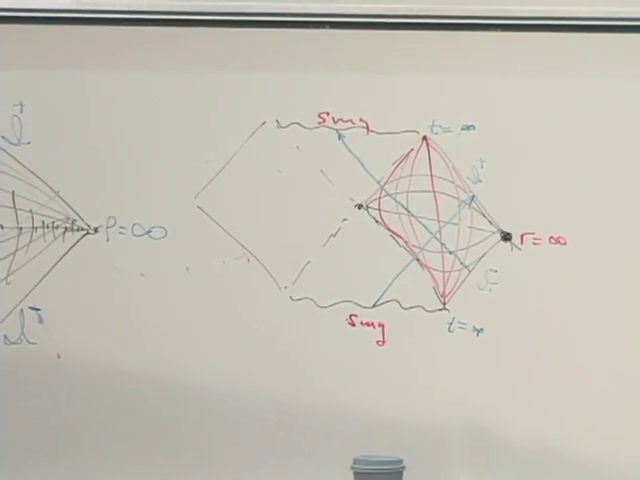
\includegraphics[width=0.74\textwidth]{lecture_04_figure_07.png}
\caption{完成した永遠のシュヴァルツシルト・ペンローズ図。特異点、事象の地平面、ヌル軌道、および一つの漸近的境界が黒板に記されている。}
\lectureframe{01:21:30.000}
\end{figure}

\begin{figure}[htbp]
\centering
\begin{tikzpicture}[scale=0.90]
\coordinate (C) at (0,0);
\coordinate (TL) at (-2,2);
\coordinate (TR) at (2,2);
\coordinate (BL) at (-2,-2);
\coordinate (BR) at (2,-2);
\coordinate (L) at (-4.0,0);
\coordinate (R) at (4.0,0);
\draw[very thick] (TL) -- (TR);
\draw[very thick] (BL) -- (BR);
\draw[thick] (C) -- (TL) (C) -- (TR) (C) -- (BL) (C) -- (BR);
\draw[thick] (TL) -- (L) -- (BL);
\draw[thick] (TR) -- (R) -- (BR);
\draw[red!75!black,very thick] (3,-1) -- (1,1) -- (0,2);
\node[above] at (0,2) {\(r=0\), future singularity};
\node[below] at (0,-2) {\(r=0\), past singularity};
\node[font=\small] at (0,1.15) {black hole};
\node[font=\small] at (0,-1.15) {white hole};
\node at (2.4,0.45) {Bob's exterior};
\node at (-2.4,0.45) {second exterior};
\node[right] at (R) {\(i^0_R\)};
\node[left] at (L) {\(i^0_L\)};
\fill (C) circle (1.5pt);
\end{tikzpicture}
\caption{永遠のシュヴァルツシルトの四つの領域。内向きの動径光線は未来の地平面を横切り、\(r=0\)で終わる。}
\label{fig:l04-eternal}
\end{figure}

\(\mathcal{I}^-\)からの内向き動径光線は未来の地平面を横切り、特異点上で終わる。上の三角形内のすべての因果曲線も同じ運命をたどる。第二の外部領域はしばしばアインシュタイン--ローゼン橋のもう一方の口として記述されるが、それは通行可能ではない。一方の外部から他方への因果的な旅を試みると、ブラックホール領域に入り、特異点に到達する。

\begin{classroomqa}
\audiencequestion{二つの外部世界はワームホールで結ばれているのか、そしてそれを通して信号を送れるのか。\lecturetimestamp{01:22:21}}
\lecturerresponse{永遠の幾何学は適切な空間的スライス上にアインシュタイン--ローゼン橋を含むが、一方の外部から他方へ因果的信号が渡ることはない。橋はあまりに急速に窄まる。地平面に入った光でさえ未来の特異点で終わる。}
\end{classroomqa}

この図は、全時間にわたって存在してきた穴を記述している。実際の天体物理学的ブラックホールは崩壊する物質から形成される。その因果図には過去のホワイトホール特異点も第二の漸近的外部もない。その幾何学を構成するには、球殻を理解する必要がある。

\section{崩壊によるブラックホールの生成}

入射粒子からなる希薄な球殻を想像せよ。それらは光子でもよい。エネルギーは重力を生むので、十分に集中した放射パルスはブラックホールを形成しうる。崩壊前、中心領域は空の平坦時空に似ている。十分なエネルギーが圧縮された後、外部はシュヴァルツシルトに似る。課題は、動く殻を挟んでこれらの領域を接続することである。

\subsection{ニュートンの球殻定理}

全質量\(M\)の球対称ニュートン球殻に対して、重力に関するガウスの法則は
\begin{equation}
\oint \mathbf{g}\cdot d\mathbf{A}=-4\pi G M_{\mathrm{enc}}.
\label{eq:l04-gauss-gravity}
\end{equation}
球対称性により\(\mathbf{g}=g(r)\hat{\mathbf r}\)なので、
\begin{equation}
g(r)=
\begin{cases}
0, & r<R_{\mathrm{shell}},\\[4pt]
-\dfrac{GM}{r^2}, & r>R_{\mathrm{shell}}.
\end{cases}
\label{eq:l04-shell-field}
\end{equation}
内部では質量が囲まれておらず、重力場は消える。外部では、球殻は中心の点質量\(M\)と全く同じように振る舞う。内部のポテンシャルはゼロではなく一定であるが、局所的なニュートン力は残らない。\editorialnote{教室で与えられた電気力線の議論は、ガウスの法則によって正確に捉えられている。場がゼロであることとポテンシャルが一定であることの区別は、相対論で時計の規格化を比較するときに重要である。}

完全に球対称な球殻が収縮する間も、その全質量が保存される限り、結論は真のままである。内部解と外部解の境界の位置だけが変わる。

\subsection{ビルクホフの定理}

相対論的な対応物はビルクホフの定理である。すべての球対称真空領域は、局所的にシュヴァルツシルト族の一部である。中心に質量を持たない球殻に対して、
\begin{align}
ds^2_{\mathrm{inside}}&=-dT^2+dR^2+R^2d\Omega_2^2,\\
ds^2_{\mathrm{outside}}&=
-\left(1-\frac{2GM}{r}\right)dt^2
\nonumber\\
&\quad+\frac{dr^2}{1-2GM/r}
+r^2d\Omega_2^2.
\label{eq:l04-birkhoff-pieces}
\end{align}

\begin{figure}[htbp]
\centering
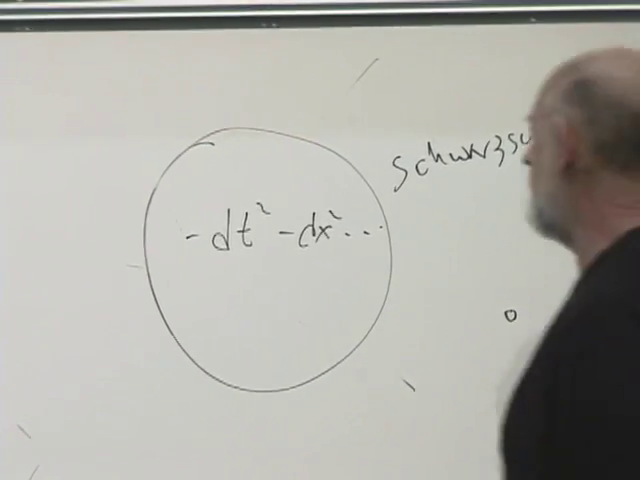
\includegraphics[width=0.74\textwidth]{lecture_04_figure_08.png}
\caption{球殻接続の黒板。円の内部は平坦時空、外部はシュヴァルツシルト解。}
\lectureframe{01:34:15.000}
\end{figure}

\begin{classroomqa}
\audiencequestion{一般相対論で球殻の外部に現れる計量は何か。\lecturetimestamp{01:33:17}}
\lecturerresponse{シュヴァルツシルト計量であり、質量パラメータは球殻の全保存質量に等しい。空の中心領域は局所的にミンコフスキー時空である。}
\end{classroomqa}

\begin{classroomqa}
\audiencequestion{殻が収縮するなら、なぜ質量パラメータは変化しないのか。\lecturetimestamp{01:34:33}}
\lecturerresponse{全エネルギーが保存されるからである。殻の半径や運動・束縛への寄与は変化しうるが、孤立した球対称系では保存される外部質量は固定されている。動く殻は、平坦領域とシュヴァルツシルト領域が接合される位置を変える。}
\end{classroomqa}

内部が平坦であることは、内部の時計が必ずしも無限遠の時計と同じ規格化をもつことを意味しない。殻をまたいだ接続により、内部時間座標が定数倍されうるし、動く殻には対応する接合条件が必要である。\editorialnote{ビルクホフの定理は各真空領域を局所的に固定する。それらの座標の大域的な関係は、殻をまたいで誘導計量と外曲率を接合することによって決まる。それらの詳細は、崩壊の構成とまったく同様に、次回の講義に先送りする。}

これで形成に必要な二つの要素がそろった。収縮する殻の内側のミンコフスキー時空と、その外側のシュヴァルツシルト時空である。殻が内側へ動くにつれ、それらの界面は世界管を描く。その管を、本来のシュヴァルツシルト半径を通り抜けて追うことにより、図~\ref{fig:l04-eternal}の非物理的な過去の半分は規則的な崩壊前領域に置き換えられ、実際のブラックホールの事象の地平面がどこで始まるかが明らかになる。

\chapter{ブラックホールの構築と近地平線パズル}

\lectureoverview{我々は三つの部品からブラックホールを構築する。すなわち、平坦時空の因果図、シュヴァルツシルト図、そして球殻に対するビルクホフの定理である。この構築により、事象の地平線が大域的な境界であり、局所的に平坦な領域から始まりうることが明らかになる。次に因果幾何学からエントロピーとホーキング温度へと移る。地平線の近くに保持された温度計はいくらでも高温になるが、自由落下する観測者は局所的な破局を予期しない。最後の議論では、外部の実験が、検出しようとする擾乱を自ら生み出すことなく、実際に何を確定できるかを問う。}

\section{真空の温度を持つブラックホール}

宿題があったはずである。ブラックホールを構築し、授業に持ってきて発表するというものである。誰も披露できるものを持っていなかったが、Wolframを通じて見つけた計算が、より穏やかな導入問題を提供した。どのような半径と質量であれば、ブラックホールのホーキング温度が宇宙マイクロ波背景放射の\(3\,\mathrm{K}\)温度に近くなるだろうか。

\begin{classroomqa}
\audiencequestion{ウェブサイトでは何が計算されたのですか。\lecturetimestamp{00:00:39}}
\lecturerresponse{温度がおよそ\(3\,\mathrm{K}\)であるブラックホールの半径です。要点は精密な計算ではなく、物理的スケールの見積もりです。}
\end{classroomqa}

そのようなブラックホールは一瞬だけ周囲と同じ温度になるが、その平衡は不安定である。シュヴァルツシルトブラックホールは負の熱容量を持つ。もしわずかに浴よりも高温になれば、放射して質量を失い、さらに高温になる。もしわずかに低温になれば、吸収して質量を増やし、さらに低温になる。\editorialnote{これが、意図的に緩やかな教室での言い回しの背後にある正確な安定性の議論である。正準熱浴は、孤立したシュヴァルツシルトブラックホールに安定な平衡を与えることができない。}

見積もりは\(3\,\mathrm{K}\)放射の特性波長から始まる。

\begin{classroomqa}
\audiencequestion{約三ケルビンの放射にはどのような波長が対応するか。\lecturetimestamp{00:02:03}}
\lecturerresponse{会場からは一センチメートル、\(21\)センチメートル、さらには\(10\)メートルという答えが挙がったが、最終的にはマイクロ波の領域に落ち着いた。この議論にとって有用な桁程度の答えは約一センチメートルであり、電子レンジやパン箱に関する冗談が出るほど小さかった。}
\end{classroomqa}

典型的なホーキング量子の波長は、数因子を除いてシュヴァルツシルト半径と同程度である。
\begin{equation}
\lambda_{\mathrm{H}}\sim R_s,
\qquad
R_s=\frac{2GM}{c^2}.
\label{eq:l05-scale}
\end{equation}
教室での値\(\lambda_{\mathrm H}\sim1\,\mathrm{cm}\)を取ると\(R_s\sim1\,\mathrm{cm}\)が得られる。太陽質量のブラックホールの半径は数キロメートルであり、\(R_s\)は\(M\)に比例するので、対応する質量はおよそ
\begin{equation}
M\sim10^{-5}M_\odot,
\label{eq:l05-rough-mass}
\end{equation}
となり、惑星規模である。これが、講義が地球程度の見積もりに到達する理由である。

\begin{classroomqa}
\audiencequestion{それはWolframによる数値結果と一致しますか。\lecturetimestamp{00:05:53}}
\lecturerresponse{報告された結果は月の質量に近かった。それは粗い見積もりに比べて小さく聞こえたが、どちらの答えでも意図された要点は成り立つ。すなわち、その物体はポケットに入れて持ち運べるものではない。}
\end{classroomqa}

定数を保持しておくと、この不一致が説明できる。
\begin{equation}
T_H=\frac{\hbar c}{4\pi k_B R_s},
\end{equation}
から、\(T_H=3\,\mathrm{K}\)において
\begin{equation}
R_s\simeq6.1\times10^{-5}\,\mathrm{m},
\qquad
M\simeq4.1\times10^{22}\,\mathrm{kg}.
\label{eq:l05-three-kelvin}
\end{equation}
が得られる。これは地球質量ではなく月質量である。マイクロ波の波長、因子\(4\pi\)、そしてどの黒体波長を典型的と呼ぶかの選択が、迅速な見積もりと数値との差を説明する。\editorialnote{式~\eqref{eq:l05-three-kelvin}は、講義の次元解析による見積もりで省略された数因子を復元する。見積もり自体は、授業で用いられた経路であるため保持されている。}

この計算はその目的を果たした。ここで我々は、数学的に、そして想像の中で、ブラックホールを構築したい。完全な場の方程式は現在の目的には難しすぎる。図が基本的な事実を与えてくれる。

\section{最初の作業部品：平坦時空}

観測者を中心とする極座標を用い、角度を抑止する。縮約された座標は\((t,r)\)であり、\(r\geq0\)である。この縮約図の点は四次元時空の点ではなく、\(r=0\)を除いて、二次元球面\(S^2\)全体を表す。

動径方向の光線は\(45^\circ\)で進む。内向きの光線は原点に到達し、外向きの光線はもう一方のヌル方向に沿って原点を離れる。無限半平面は、共形変換によって有限のペンローズ楔へと圧縮できる。この変換は一意ではない。その本質的な性質は、無限遠が有限の境界へもたらされることと、動径方向のヌル方向が\(45^\circ\)に保たれることである。黒板の言葉で言えば、我々は図を押しつぶすのである。

\begin{figure}[htbp]
\centering
\includegraphics[width=0.68\textwidth]{lecture_05_figure_02.png}
\caption{コンパクト化された動径ミンコフスキー時空の上半分。垂直な辺は\(r=0\)であり、一方、曲線族はコンパクト化された無限遠に向かって密集している。}
\lectureframe{00:11:41.560}
\end{figure}

\begin{figure}[htbp]
\centering
\begin{tikzpicture}[scale=0.94]
\coordinate (O) at (0,0);
\coordinate (P) at (0,3.8);
\coordinate (I) at (6.2,1.9);
\draw[very thick] (O)--(P)--(I)--cycle;
\foreach \y in {0.45,0.90,1.35,1.80,2.25,2.70,3.15} {
  \draw[gray!75] (0,\y) .. controls (2.0,\y-0.18) and (4.4,1.9) .. (I);
}
\draw[gray!75] (0.65,0.37) .. controls (1.55,1.20) and (1.55,2.60) .. (0.65,3.43);
\draw[gray!75] (1.30,0.74) .. controls (2.25,1.30) and (2.25,2.50) .. (1.30,3.06);
\draw[gray!75] (2.05,1.08) .. controls (3.00,1.46) and (3.00,2.34) .. (2.05,2.72);
\draw[gray!75] (3.00,1.36) .. controls (3.85,1.62) and (3.85,2.18) .. (3.00,2.44);
\node[left] at (0,1.9) {\(r=0\)};
\node[above] at (P) {\(i^+\)};
\node[right] at (I) {\(i^0\)};
\end{tikzpicture}
\caption{上部楔形の簡略版。曲線は定性的な定\(r\)および定\(t\)の族であり、正確な座標格子ではない。}
\label{fig:l05-flat-wedge}
\end{figure}

\(r\)を固定した世界線は、コンパクト化前は垂直であり、未来の時間的無限遠の近くで湾曲して蓄積する。定\(t\)のスライスも同様に空間的無限遠に向かって密集する。この密集は座標効果であり、物質の物理的な圧縮ではない。

\(45^\circ\)の規則は動径方向の光に直接適用される。角運動量をもつ光線は原点を外れ、ゼロでない最近接距離に達し、外向きに戻ることがある。原点から遠くでは、その射影された運動はほとんど動径的に見える。最近接の近くでのみ、還元された\((t,r)\)軌道が目に見えて曲がる。これで最初の作業部分は完了する。

\section{第二の作業部分：永遠のシュヴァルツシルト}

最大拡張シュヴァルツシルト解は、二つの外部ダイヤモンド、未来のブラックホール領域、および過去のホワイトホール領域をもつ。その上下の波状の境界は、未来および過去の特異点である。崩壊によって作られたブラックホールでは、この構造の大部分はまもなく捨てられるが、通常の右側の外部はまさに我々が必要とする部分である。

\begin{figure}[htbp]
\centering
\includegraphics[width=0.72\textwidth]{lecture_05_figure_03.png}
\caption{永遠のシュヴァルツシルト図。右側に通常の外部とその概略的な座標格子を示す。}
\lectureframe{00:16:55.975}
\end{figure}

\begin{figure}[htbp]
\centering
\begin{tikzpicture}[scale=0.88]
\coordinate (C) at (0,0);
\coordinate (TL) at (-2.0,2.0);
\coordinate (L) at (-4.0,0);
\coordinate (BL) at (-2.0,-2.0);
\coordinate (TR) at (2.0,2.0);
\coordinate (R) at (4.0,0);
\coordinate (BR) at (2.0,-2.0);
\draw[thick] (C)--(TL)--(L)--(BL)--(C);
\draw[thick] (C)--(TR)--(R)--(BR)--(C);
\draw[very thick,decorate,decoration={snake,amplitude=1.2pt,segment length=7pt}] (TL)--(TR);
\draw[very thick,decorate,decoration={snake,amplitude=1.2pt,segment length=7pt}] (BL)--(BR);
\draw[gray!75] (TR) .. controls (2.15,0.8) and (2.15,-0.8) .. (BR);
\draw[gray!75] (TR) .. controls (2.65,0.9) and (2.65,-0.9) .. (BR);
\draw[gray!75] (TR) .. controls (3.20,0.7) and (3.20,-0.7) .. (BR);
\draw[gray!75] (0.15,0.95) .. controls (1.5,0.82) and (2.9,0.40) .. (R);
\draw[gray!75] (0.10,0.35) .. controls (1.5,0.34) and (2.9,0.18) .. (R);
\draw[gray!75] (0.10,-0.35) .. controls (1.5,-0.34) and (2.9,-0.18) .. (R);
\fill (C) circle (1.6pt);
\node[above] at (TR) {\(i^+\)};
\node[below] at (BR) {\(i^-\)};
\node[right] at (R) {\(i^0,\ r=\infty\)};
\node[above] at (0,2.25) {\(r=0\), future singularity};
\node[below] at (0,-2.25) {\(r=0\), past singularity};
\node[rotate=45,above,font=\small] at (1.0,1.0) {\(r=2GM\)};
\node[font=\small] at (2.70,0.75) {\(r=6GM\)};
\node[font=\small] at (3.15,-0.75) {\(r=100GM\)};
\end{tikzpicture}
\caption{右側の外部は、大きな半径では平坦な楔形に似ている。その内側のヌル辺は\(c=1\)のとき\(r=2GM\)である。他のラベル付けされた半径は概略的な例である。}
\label{fig:l05-eternal-schwarzschild}
\end{figure}

ブラックホールから遠くでは、外部はますますコンパクト化された平坦空間のように見える。\(r=6GM\)や\(r=100GM\)のような線は、通常の定半径世界線の振る舞いに近づく。外部の内側の境界は
\begin{equation}
r=2GM
\end{equation}
であり、単位は\(c=1\)である。

中心の近くでは、平坦空間との比較は成り立たない。ミンコフスキー空間の動径光線は\(r=0\)に達し、反対側の物理的な側から再び現れる。シュヴァルツシルト内部の未来向き光線は跳ね返らない。それは\(r=0\)の空間的特異点で終わる。この因果的な違いこそ、崩壊の構成が保たなければならないものである。

\section{部分をつなぎ合わせることを可能にする定理}

欠けている要素はまずニュートン重力に現れる。球対称な質量分布に対して、ガウスの法則は
\begin{equation}
\oint\mathbf g\cdot d\mathbf A=-4\pi G M_{\mathrm{enc}},
\end{equation}
を与え、したがって
\begin{equation}
\mathbf g(r)=-\frac{G M_{\mathrm{enc}}(r)}{r^2}\,\hat{\mathbf r}.
\label{eq:l05-shell-theorem}
\end{equation}
となる。半径\(r\)の球の外側の物質は、そこに正味の場を寄与しない。全質量\(M\)の中空の殻に対しては、
\begin{equation}
\mathbf g=
\begin{cases}
0, & r<R_{\mathrm{shell}},\\[3pt]
-\dfrac{GM}{r^2}\hat{\mathbf r}, & r>R_{\mathrm{shell}}.
\end{cases}
\end{equation}

ビルクホフの定理はその相対論的な置き換えである。すべての球対称真空領域は、定数質量パラメータをもつ局所的なシュヴァルツシルト領域である。球殻の空の内部は質量パラメータがゼロで局所的にミンコフスキーであり、外部は質量パラメータ\(M\)をもちシュヴァルツシルトである：
\begin{equation}
\begin{aligned}
M_{\mathrm{enc}}&=0 && \text{inside the shell},\\
M_{\mathrm{enc}}&=M && \text{outside the shell}.
\end{aligned}
\label{eq:l05-birkhoff}
\end{equation}
この主張は殻が動いている間も有用であり続ける。なぜなら、両側の真空領域は球対称のままだからである。

\editorialnote{内部が平坦であることは局所的な主張である。静的な殻は、内部の曲率が消えていても、内部時間座標の規格化を変えうる。動く殻またはヌル殻に対しては、二つの真空計量を殻を挟んで接合しなければならない。理想化された構成は薄殻接合であり、内向きヴァイディヤ幾何と密接に関係している。これらの但し書きはいずれも、ここで用いられる因果的な切り貼り議論を変えない。}

実験室のイメージとしては、大きな慣性閉じ込め施設のように、同期したレーザーで密に覆われた球を想像し、それらをすべて一度に内向きに発射する。理想化では装置はなく、完全に球形の光の殻だけがある。殻はエネルギー\(E\)を運ぶので、外部の質量パラメータは
\begin{equation}
M=\frac{E}{c^2},
\end{equation}
であり、自然単位では単に\(E=M\)である。殻は光速で動くので、還元図上では内向きのヌル線である。その線上の各点は一つの光子の軌道ではなく、球面波面全体を表す。

\section{崩壊時空を縫い合わせる}

平坦な時空から始め、内向きのヌル殻を描く。殻の内側の領域は正しい。ビルクホフの定理によりそれは平坦である。外側の領域は正しくない。なぜなら、外部はそのシュヴァルツシルト幾何を通じて、すでに殻の全質量を知っていなければならないからである。

次に、同じ殻を永遠シュヴァルツシルト図に描こう。そこでは、殻の外側の領域は正しい。白色穴、第二の外部、そしてブラックホール内部の不適切な部分は、通常の空っぽの空間で始まる崩壊にとっては誤りであるから、それらを消去する。

\begin{figure}[htbp]
\centering
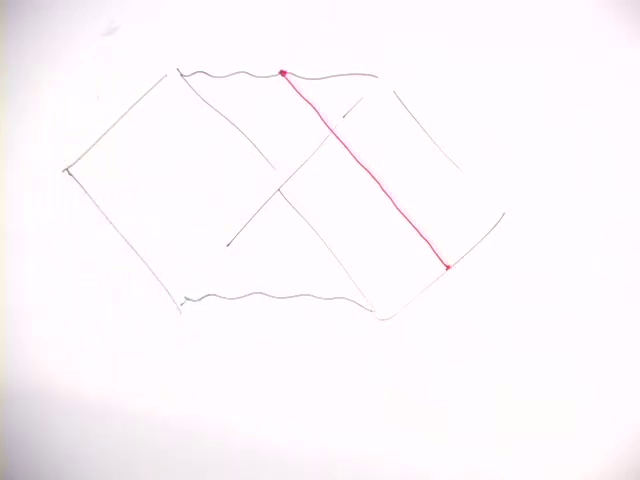
\includegraphics[width=0.72\textwidth]{lecture_05_figure_05.png}
\caption{赤で示されたヌル殻が、正しい外部部分を切り出しつつシュヴァルツシルト図全体に描かれている。}
\lectureframe{00:32:00.000}
\end{figure}

殻は平坦な部分において\(r=0\)に到達する。シュヴァルツシルト部分では、未来の特異点の始まりに到達する。これらは同じ端点である。平坦な内部を殻に沿ってシュヴァルツシルト外部に貼り合わせると、ブラックホール形成の最も単純な時空が得られる。

\begin{classroomqa}
\audiencequestion{左上の接合点において、平坦空間の端点は本当にシュヴァルツシルト側の点と同じなのですか。\lecturetimestamp{00:34:50}}
\lecturerresponse{はい。平坦空間の殻は\(r=0\)に収縮し、シュヴァルツシルト特異点もまた\(r=0\)にある。同定される二つの点は同じ幾何学的意味を持つ。すなわち、二次元球面が大きさゼロに収縮しているのである。}
\end{classroomqa}

\begin{figure}[htbp]
\centering
\begin{tikzpicture}[scale=0.96]
\coordinate (A) at (0,-2.8);
\coordinate (B) at (0,1.65);
\coordinate (C) at (2.05,1.65);
\coordinate (D) at (5.4,-0.15);
\coordinate (E) at (3.75,3.10);
\coordinate (H0) at (0,-0.45);
\draw[very thick] (A)--(B);
\draw[very thick] (A)--(D)--(E);
\draw[very thick,red!75!black] (D)--(B);
\draw[very thick,decorate,decoration={snake,amplitude=1.2pt,segment length=7pt}] (B)--(C);
\draw[very thick,green!45!black] (H0)--(C);
\draw[thick] (C)--(E);
\node[left] at (0,0.45) {\(r=0\)};
\node[below right] at (3.95,-0.05) {ingoing null shell};
\node[font=\small] at (1.25,-1.35) {flat interior};
\node[font=\small,anchor=west] at (2.55,2.38) {Schwarzschild exterior};
\node[above,font=\small] at (1.0,2.02) {\(r=0\) singularity};
\node[above left,font=\small] at (0.98,0.62) {event horizon};
\node[right] at (E) {\(i^+\)};
\end{tikzpicture}
\caption{崩壊の幾何。赤い殻は平坦な内部とシュヴァルツシルト外部を接合する。緑の事象の地平面は平坦領域においてより早く始まり、ブラックホール領域の未来境界で終わる。}
\label{fig:l05-collapse}
\end{figure}

この構成は、永遠解が残した問いに答える。崩壊から作られたブラックホールには、過去の白色穴も第二の漸近宇宙もない。それでも未来の特異点は持つ。

\section{地平面は大域的な境界である}

古いラベル\(r=2GM\)は、定常シュヴァルツシルト幾何において地平面を同定したが、それは動的時空で必要とされる定義ではない。

\begin{definition}
未来事象の地平面とは、未来向きの因果的信号を未来ヌル無限遠へ送ることができる事象の集合の境界である。
\end{definition}

崩壊図上で、ちょうど脱出に失敗する外向きヌル光線をたどろう。そのすぐ外側の光線は無限遠に到達し、すぐ内側の光線は特異点で終わる。その分離線が真の地平面である。

\begin{figure}[htbp]
\centering
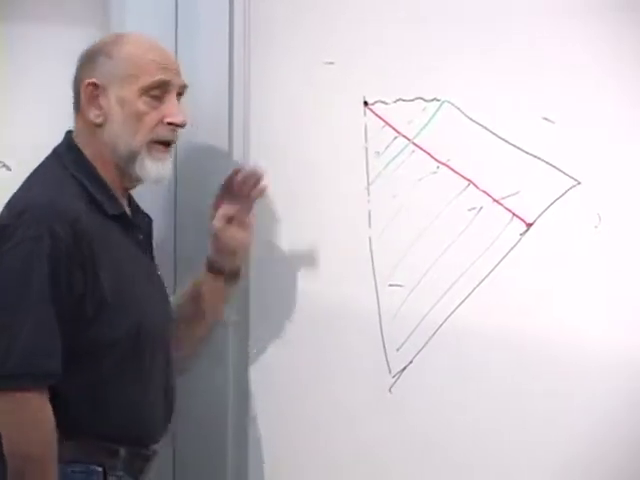
\includegraphics[width=0.72\textwidth]{lecture_05_figure_06.png}
\caption{完成した黒板の構成。入射する殻は赤、事象の地平面は緑であり、緑の線の一部は殻の下のまだ平坦な領域にある。}
\lectureframe{00:39:10.000}
\end{figure}

驚くべき特徴はもはや避けられない。地平面は、殻がまだ到着していない領域へと後方に延びている。そこの幾何は局所的に平坦であり、その線を横切る観測者は曲率のパルス、壁、閃光を検知しない。それにもかかわらず、その観測者はすでに無限遠に到達できない。なぜなら、未来の殻が可能な脱出経路をすべて閉ざすからである。事象の地平面はまさにこの大域的な意味で目的論的である。すなわち、それを見つけるには時空の未来全体の知識が必要である。\editorialnote{滑らかな事象の地平面をちょうど横切ったことを局所実験で決定することはできない。見かけの地平面やトラッピング地平面など他の概念はより局所的であり、崩壊の間、事象の地平面と一致する必要はない。}

排水口の類推は因果的考えを際立たせる。動かない湖の栓をした排水口の近くに漕ぎ手を想像しよう。栓が永遠に残るなら、漕ぎ手は去ることができる。誰かが必ず栓を抜くなら、まだ水が動いていなくても、後の流れが脱出を不可能にするかもしれない。凍結したナイアガラの滝も同じ点を示す。穏やかな水は安全への未来の経路を保証しない。

\begin{classroomqa}
\audiencequestion{光の球面殻がますます集中するから栓が抜かれるのですか。\lecturetimestamp{00:43:13}}
\lecturerresponse{その集中がブラックホールを創るが、排水口の話はより狭い目的で使われている。すなわち、局所的に劇的なことが何も起こる前に、すでに引き返せない点を越えていることがありうるのである。}
\end{classroomqa}

\subsection{成長する球面からなる地平面}

縮約された地平面の各点は\(S^2\)を表す。地平面の最初の点では、その球面は面積ゼロである。地平面に沿って上へ進むと、球面は成長し、その面積半径が
\begin{equation}
R_s=\frac{2GM}{c^2}.
\end{equation}
に達する。定常ブラックホールではその大きさにとどまり、さらにエネルギーが落下すれば再び成長する。

\editorialnote{理想化された球対称崩壊図では、地平面の生成子は\(r=0\)上の形成点、すなわち折り目で出会う。面積ゼロなのはこの極限の二次元球面であり、この記述は有限のシュヴァルツシルト地平面が突然一点に収縮すると読まれるべきではない。}

\subsection{遠方の観測者が再構成できること}

続く長い議論は、すでに大域的地平面の内側にいる観測者と、その観測者がそこに至るまでの歴史とを分ける。

\begin{classroomqa}
\audiencequestion{殻が到着する前に閉じ込められた人の状態はどうなっているのか。遠方の観測者から見て、その人は事象の地平面の外にいるのか。\lecturetimestamp{00:44:03}}
\lecturerresponse{いいえ。世界線が事象の地平面の背後に入ってしまえば、その未来は特異点に達し、そこから新たな信号が遠方の観測者に届くことはない。しかし、その人がそこで存在し始めたわけではない。それ以前の粒子、祖先、あるいは他の先行するエネルギーは、可視であった領域から入ってきたのである。}
\end{classroomqa}

したがって遠方の観測者は、先行する物質が地平面に近づくのを見ることができるが、その向こうから信号を受け取ることは決してない。到来する殻を通して見ることに矛盾はない。殻は光でできており、観測者は殻そのものも見て、ブラックホールが形成されたと推論できるのである。

\begin{classroomqa}
\audiencequestion{視線は崩壊する殻を通過するのか、そして外部の観測者は依然として穴が形成されたことを知ることができるのか。\lecturetimestamp{00:46:51}}
\lecturerresponse{はい。観測者は到来する殻を見ており、その光がまだ脱出できるうちに殻を横切る経路の光を受け取ることができる。奇妙に見えるのは、殻が中心に達する前から先行する物質が新たに定まった地平面に近づくことである。}
\end{classroomqa}

\begin{classroomqa}
\audiencequestion{これは、外部から見ると物質が地平面に圧縮されたように見えるという規則の続きなのか。\lecturetimestamp{00:47:49}}
\lecturerresponse{はい。外部記述では、物質は地平面に付随したままで、ますます赤方偏移し、やがてブラックホール蒸発という後の量子過程が話を変えるまで続く。}
\end{classroomqa}

この外部記述が次の主題を動機づける。情報が二次元の表面に貼り付けられているように見えるなら、ブラックホールのエントロピーがその表面の面積に比例することは、それほど驚くべきことではない。

\section{エントロピーと無限遠から見た温度}

大きな地平面の近くでは、小さな実験室で平坦地球近似を用いるのと同様に、球面を局所的な平面で置き換えてよい。そこで、以前の議論からの二つの事実が結び合わされる。
\begin{equation}
\begin{aligned}
S_{\mathrm{BH}}&\propto A_H,\\
\Delta A_H&\sim \ell_P^2
\quad\text{per added bit, schematically}.
\end{aligned}
\end{equation}
プランク面積あたり1ビットという記憶法は面積則を表しており、微視的な導出ではない。

シュヴァルツシルトブラックホールから遠く離れて測ったホーキング温度は
\begin{equation}
T_H=\frac{\hbar c^3}{8\pi GMk_B}.
\label{eq:l05-hawking}
\end{equation}
\(R_s=2GM/c^2\)を用いると、
\begin{equation}
T_H=\frac{\hbar c}{4\pi k_B R_s}.
\label{eq:l05-hawking-radius}
\end{equation}
したがって、より大きな穴はより冷たい。

\begin{classroomqa}
\audiencequestion{温度は位置に依存しうるのか。\lecturetimestamp{00:52:43}}
\lecturerresponse{日常的な会話では明らかに依存しうる。ニューヨークとスタンフォードが同じ温度である必要はない。より鋭い問いは、重力熱平衡にある系についてである。そこでは、赤方偏移した平衡温度が一定であっても、局所的な温度計の読みは高さによって変わりうる。}
\end{classroomqa}

温度は局所的な運動エネルギーを通して読み取られる。熱せられた地球の上の希薄な大気では、分子は上昇するにつれて運動エネルギーを失い、下降するにつれて得る。光子は上向きに赤方偏移し、下向きに青方偏移する。したがって、低い温度計と高い温度計は同じ局所的なエネルギー尺度を示す必要はない。

静的時空に対して、平衡関係は
\begin{equation}
T_{\mathrm{loc}}(r)\sqrt{-g_{tt}(r)}=T_\infty,
\label{eq:l05-tolman}
\end{equation}
すなわちトルマンの法則である。式~\eqref{eq:l05-hawking}のホーキング温度は\(T_\infty\)であり、無限遠で規格化された読みである。

\section{地平面近くの高温の静的雰囲気}

\(\rho\)を地平面から外向きの固有距離とする。大きなシュヴァルツシルト地平面の近くでは、式~\eqref{eq:l05-tolman}は
\begin{equation}
k_B T_{\mathrm{loc}}(\rho)
\simeq\frac{\hbar c}{2\pi\rho},
\label{eq:l05-local-temperature-si}
\end{equation}
となる。あるいは、単位\(c=\hbar=k_B=1\)では、
\begin{equation}
T_{\mathrm{loc}}(\rho)=\frac{1}{2\pi\rho}.
\label{eq:l05-local-temperature}
\end{equation}

\begin{figure}[htbp]
\centering
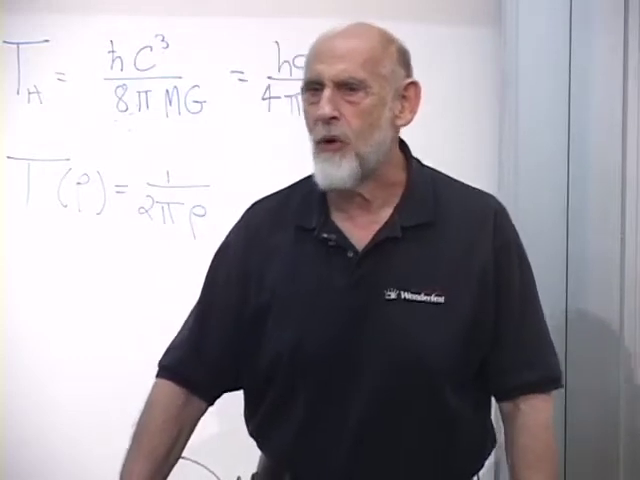
\includegraphics[width=0.72\textwidth]{lecture_05_figure_07.png}
\caption{漸近的なホーキング温度と、黒板に示された地平面近くの局所温度\(T(\rho)=1/(2\pi\rho)\)。}
\lectureframe{01:02:40.000}
\end{figure}

ケーブルで固定された\(\rho\)に保持された微小な温度計は、降ろされるにつれて上昇する温度を示す。その静的雰囲気中に保たれた原子は励起され、次に電離し、次に解離する。さらに大きな局所エネルギーでは、原子核やハドロンさえも無傷ではいられなくなる。人を足から先に降ろすと、記憶に残る診断が得られる。熱い足である。

\emph{保持された}という語が本質的である。この発散は、加速度によって静止させられた検出器に属する。それは外部時間に対して赤方偏移した熱的雰囲気を記述する。自由落下する検出器は異なる軌道をたどり、正則な量子状態にある十分大きな穴に対しては、地平面で発散する熱浴に出会う必要はない。\editorialnote{この区別は、静的観測者に見られるトルマン温度および加速度温度を、自由落下観測者の正則な局所経験から分かつ。講義はこの対比を、用語だけで解決するのではなく、意図的に操作的なパズルに変えている。}

電離の閾値がこの衝突を具体的にする。

\begin{classroomqa}
\audiencequestion{水素を電離するにはどれだけのエネルギーが必要か。\lecturetimestamp{01:06:53}}
\lecturerresponse{講義では\(13\)電子ボルトと答えられ、\(13.6\,\mathrm{eV}\)基底状態の電離エネルギーを正しく同定している。付随する数千ケルビンという見積もりは小さすぎるが、この議論には有限なしきい値が存在することだけが必要である。}
\end{classroomqa}

実際、
\begin{equation}
\frac{13.6\,\mathrm{eV}}{k_B}\simeq1.58\times10^5\,\mathrm{K}.
\end{equation}
したがって、静的温度が電離のスケールに達する小さな固有距離\(\rho_{\mathrm{ion}}\)が存在する。静的な外挿によれば、地平線の外側にあるその地点で原子はすでに電離しているはずである。これに対して自由落下する原子は、局所的な壁を予期せず、有限の固有時間で地平線を横切ることができる。外部の観測者は、これらの記述のどちらが正しいかを決める実験を行えるだろうか。

\section{ハイゼンベルクの顕微鏡}

この問いをブラックホールに適用する前に、光子顕微鏡を思い出そう。分解能\(\Delta x\)で粒子の位置を特定するには、探査波長は次を満たさなければならない。
\begin{equation}
\lambda\lesssim\Delta x.
\end{equation}
そのとき一つの光子は少なくとも次の運動量を運ぶ。
\begin{equation}
p_\gamma\gtrsim\frac{\hbar}{\Delta x}.
\label{eq:l05-microscope}
\end{equation}
その光子を散乱すると、同程度の反跳が生じる。まず位置を測定し、直ちに速度を調べると、二番目の測定は最初の測定によって変化した状態を見ることになる。実験は、排除しようとした条件を自ら作り出してしまう。

\begin{figure}[htbp]
\centering
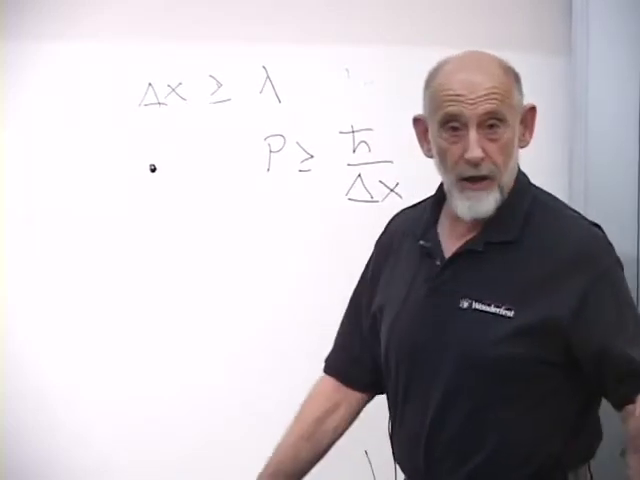
\includegraphics[width=0.70\textwidth]{lecture_05_figure_08.png}
\caption{顕微鏡は\(\Delta x\gtrsim\lambda\)および\(p_\gamma\gtrsim\hbar/\Delta x\)を見積もる。}
\lectureframe{01:11:50.000}
\end{figure}

これは単に古典光学の限界ではない。古典波はいくらでも弱くできるが、量子力学では検出が成功する事象に少なくとも一つの量子が必要である。したがって空間分解能を改善すれば、有限の運動量移行が不可避となる。

\section{地平線近傍の実験}

ここで、\(\rho_{\mathrm{ion}}\)から始まる層を原子が落下するとしよう。静的系に対して、それはほぼ\(c\)で内向きに運動しているので、地平線を横切るまでに利用できる間隔は次の程度である。
\begin{equation}
\Delta\tau\sim\frac{\rho_{\mathrm{ion}}}{c}.
\label{eq:l05-fall-time}
\end{equation}
横切った後は、いかなる結果も外部へ送り返すことはできない。測定は、この短い間隔の間に、無傷の原子と電離した原子を区別しなければならない。

層内で原子を分解するには次が必要である。
\begin{equation}
\lambda\lesssim\rho_{\mathrm{ion}}.
\end{equation}
したがって探査エネルギーは次で上限を付けられる。
\begin{equation}
E_\gamma=cp_\gamma
\gtrsim\frac{\hbar c}{\rho_{\mathrm{ion}}}.
\label{eq:l05-probe-energy}
\end{equation}
因子\(2\pi\)を除けば、これは式~\eqref{eq:l05-local-temperature-si}と同じスケールである。
\begin{equation}
E_\gamma\gtrsim2\pi k_B T_{\mathrm{loc}}(\rho_{\mathrm{ion}}).
\label{eq:l05-probe-temperature}
\end{equation}
事象を分解するのに十分なエネルギーを持つ光子は、原子を電離するのにも十分なエネルギーを持つ。

\begin{figure}[htbp]
\centering
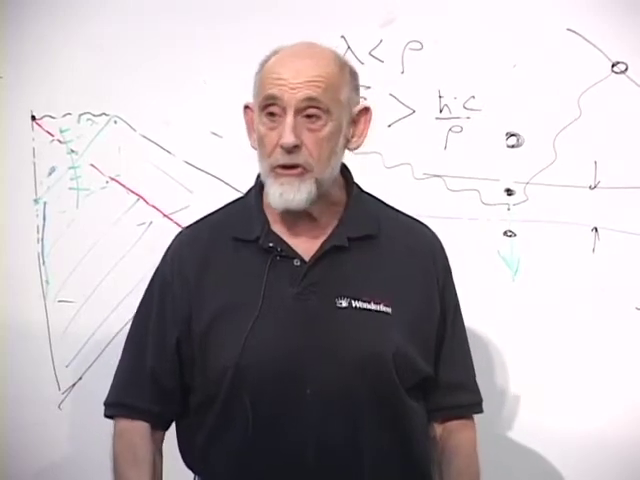
\includegraphics[width=0.72\textwidth]{lecture_05_figure_09.png}
\caption{黒板での地平線近傍の見積もり：\(\lambda<\rho\)は\(\hbar c/\rho\)程度の局所探査エネルギーを強制する。}
\lectureframe{01:18:30.000}
\end{figure}

\begin{classroomqa}
\audiencequestion{その高エネルギー光子は、自由落下系においてさえ原子を電離するだろうか。\lecturetimestamp{01:19:07}}
\lecturerresponse{はい。原子は実在の高エネルギー量子に衝突され、自身の局所系で反跳するか電離する。測定は乱されていない落下を明らかにするのではなく、それを乱された落下に置き換える。}
\end{classroomqa}

\begin{classroomqa}
\audiencequestion{原子が単に落下し、誰も実験を行わない場合はどうか。\lecturetimestamp{01:19:39}}
\lecturerresponse{その場合、この特定の擾乱は存在しない。外部の観測者が実際に高分解能の実験を行えば、原子は厄介なことになる。この議論は外部から検証できることに関するものであり、測定されない落下者が燃えることの証明ではない。}
\end{classroomqa}

\subsection{温度計や送信機の方がよりうまくできるだろうか。}

装置を移動しても情報の問題は解消しない。

\begin{classroomqa}
\audiencequestion{もっと遠くで測定し、勾配を推測し、あるいは自由落下する温度計に温度を記録させて後で回収することはできるだろうか。\lecturetimestamp{01:19:51}}
\lecturerresponse{地平線近傍の記録を知るには、何かが温度計と相互作用し、量子として情報を返さなければならない。温度計を引き返させるには激しい加速度が必要であり、遠隔で読み取るには放出か散乱が必要である。どちらの経路も、乱されていない履歴を検証しようとしていた物理系を変化させる。}
\end{classroomqa}

\begin{classroomqa}
\audiencequestion{小さな分解能に必要な高い探査エネルギーは、反射された観測を地平線近傍領域から遠ざけるのと同じ困難だろうか。\lecturetimestamp{01:21:51}}
\lecturerresponse{それらは同じ赤方偏移したスケールの両面である。光子は最終的に無限遠に達するときには低いエネルギーでありうる。なぜなら外へ登る間にエネルギーを失うからであるが、原子を分解する場所では高い局所振動数を持たなければならない。}
\end{classroomqa}

\editorialnote{地平線のすぐ外側で放出された光子は、単に脱出するためだけに大きなエネルギーを持つ必要はない。ここでの決定的な要件は、それが\(\rho\)程度の固有時間と距離のうちに事象を符号化することであり、重力赤方偏移がその大きな局所振動数をはるかに小さな漸近的振動数に関係づける。}

\begin{classroomqa}
\audiencequestion{物体が外部の光子に打たれるのではなく、自ら情報を放出することはできるのか。\lecturetimestamp{01:22:51}}
\lecturerresponse{できる。しかし、その局所的な放出にも、短い間隔の間に何が起きたかを同定するのに必要な帯域幅は依然として必要である。放出はまた、物体に反跳を与える。反射光を送信機で置き換えても、無コストの記録が得られるわけではない。}
\end{classroomqa}

\begin{classroomqa}
\audiencequestion{落下する原子には優先的な方向がある。その向きを持った運動エネルギーが温度と呼ばれているのか。\lecturetimestamp{01:23:10}}
\lecturerresponse{いいえ。野球ボールを投げても野球ボールは熱くならない。バルクの落下エネルギーと熱的揺らぎは別物である。この議論における温度は、原子の重心運動ではなく、周囲の静的放射大気に属するものである。}
\end{classroomqa}

\begin{classroomqa}
\audiencequestion{共に落下する実験室が磁場を用いて、原子が電離しているかどうかを調べることはできるか。\lecturetimestamp{01:23:50}}
\lecturerresponse{実験室は局所的な測定を行うことができる。困難は、地平線を横切る前にその結果を外部へ伝えることにある。その通信にもまた、相互作用と、必要な局所分解能を持つ外向きの量子が必要である。}
\end{classroomqa}

\begin{classroomqa}
\audiencequestion{温度計に組み込まれた送信機は、装置を破壊してしまうほど多くの局所エネルギーを必要とするのか。\lecturetimestamp{01:24:57}}
\lecturerresponse{それは同じ障害を工学的な形で表したものである。地平線に十分近づくと、関連する局所スケールで必要となる信号エネルギーは、測定しようとしている熱的スケールと同程度になる。}
\end{classroomqa}

\begin{classroomqa}
\audiencequestion{高温領域は、ゆっくり測定を行う時間がないほど薄いのか。\lecturetimestamp{01:25:15}}
\lecturerresponse{そのとおり。その固有の厚さは\(\rho\)の程度であり、横断時間は\(\rho/c\)の程度である。この制限は空間分解能としても時間帯域幅としても記述できるが、どちらの記述でも高い局所運動量またはエネルギーを要求する。}
\end{classroomqa}

対応する時間帯域幅の評価は
\begin{equation}
\Delta E\,\Delta\tau\gtrsim\hbar.
\end{equation}
である。ここではこれはフーリエ分解能または操作的な分解能の限界として読まれるべきであり、\(\Delta x\,\Delta p\geq\hbar/2\)と同一の地位を持つ演算子の不確定性関係としてではない。講義は時間とエネルギーの不確定性を発見法的に用いている。空間分解能から導かれた式~\eqref{eq:l05-probe-energy}が、この議論のより堅固な部分である。

\begin{classroomqa}
\audiencequestion{より低エネルギーで低分解能のプローブを多数の原子に用い、統計的に答えを回復することはできるか。\lecturetimestamp{01:26:26}}
\lecturerresponse{これはもっともな問いであり、教室では未解決のままにされている。各原子はただ一度の通過しか与えず、回復される信号は依然として、地平線近傍の短い事象を同定するのに十分な情報を運ばなければならない。講義は不確定性原理に訴えているが、完全な統計的ノーゴー証明を与えてはいない。}
\end{classroomqa}

\enlargethispage{2\baselineskip}
\section{何が確立され、何が確立されていないか}

この議論は、自由落下する人が発散する静的温度を感じなければならないと予測しているのではない。

\begin{classroomqa}
\audiencequestion{落下する人は温度を感じないと予測できると言っているのか。\lecturetimestamp{01:27:38}}
\lecturerresponse{いいえ。結論はもっと狭い。原子が高温の擾乱を経験しなかったことを確認するために設計された外部の実験は、同じスケールの擾乱を生み出す、ということである。この操作的解析が確立するのはそれだけである。}
\end{classroomqa}

したがって結論は、ファイアウォール定理でも、落下者が焼かれることの証明でも、何も起こらないことの証明でもない。それは外部からの検証に対する限界である。すなわち、\emph{擾乱されていない地平線近傍の事象を分解するには、それを擾乱するプローブが必要である}。
実験を行えば、その量子は、試験しようとしていた効果を生み出す。実験を行わなければ、この議論だけでは、実験的にアクセス可能な追加の事実を何も与えない。二重スリット実験との比較は意図的なものである。経路測定なしにどちらのスリットを通ったかを問うことと、相互作用なしに外部装置が何を証明するかを問うことは、どちらも、提案された証拠が得られないところに操作的な答えを結びつけようとする試みである。

\chapter{長い弦とブラックホール対応}

\lectureoverview{ブラックホールはエントロピーをもつので、微視的自由度をもたなければならない。我々はそれらの自由度について最も単純な弦理論的説明を構成する。まず長く励起された弦の状態を数え、次に弦結合定数を変化させて、弦とブラックホールの記述が出会うところを探る。最後の等号は、次の講義で完成させるべき問題として意図的に残しておく。}

\section{エントロピーは微視的担い手を要求する}

系が大きなエントロピーをもつということは、それが大量の微視的情報を隠しうるということである。熱い湯を張った浴槽は程度\(10^{30}\)のエントロピーをもちうる。この言明は、我々がそれを分子ごとに調べることを選ぶかどうかにかかわらず、膨大な数の微視的自由度が存在することをすでに告げている。熱力学はエネルギーと温度を測定することによってエントロピーを決定できるが、それを担う対象を特定するわけではない。

流体力学はこの区別を身近なものにする。それは原子に言及することなく、密度、速度、圧力、巨視的流れを記述する。熱力学を加えると、流体がエントロピーをもつことがわかる。エントロピーは、粗視化された方程式が示さない微視的構造を告げ知らせる。それは答えを与えるのではなく、新たな問いを招くのである。

ブラックホールは同じ難題をより鋭い形で提示する。ベッケンシュタインの提案は、ホーキングの計算によって完成され、地平線面積に比例するエントロピーを割り当てる。一般相対性理論は幾何とその熱力学を決定するが、微視的状態の目録を与えることはない。面積則を説明する配置をもつ、小さく多数の対象とは何か。弦理論には具体的な候補がある。ここで展開する議論は意図的に定性的である。それは数値定数や完全な状態数の形式的機構を抑えつつ、パラメータ依存性を正しく捉える。

\section{三つのスケールと一つの記法上の危険}

重力は特別な長さ、すなわちプランク長を与える。
\begin{equation}
\ell_p=\sqrt{\frac{G_N\hbar}{c^3}}.
\label{eq:l06-planck-si}
\end{equation}

\begin{classroomqa}
\audiencequestion{\(G_N\)、\(\hbar\)、\(c\)のどの組み合わせがプランク長を与えるか。\lecturetimestamp{00:06:08}}
\lecturerresponse{それは\(\sqrt{G_N\hbar/c^3}\)であり、およそ\(10^{-33}\)センチメートルである。我々は直ちに\(\hbar=c=1\)と置くので、関係はずっと簡単になる。}
\end{classroomqa}

自然単位では、
\begin{equation}
\hbar=c=1,
\qquad
G_N=\ell_p^2.
\label{eq:l06-planck-area}
\end{equation}
したがってニュートン定数は面積の次元をもつ。これが、面積を\(G_N\)で割ったものが無次元であり、エントロピーになりうる理由である。

弦理論には第二の長さ\(\ell_s\)がある。弦を熱するか、あるいは高度に励起された状態に置くと、それは多くのスケールで揺れる。この初等的な描像における特徴的な最短スケールは弦の長さである。\(\ell_s\)を、弦振動の一つの素励起単位に付随する大きさとみなしてよい。

第三の量は無次元の弦結合定数\(g_s\)である。それは分裂と結合を支配する。弦は二本の弦にくびれて分かれることができ、あるいは励起された弦は閉弦量子を放出できる。

\begin{classroomqa}
\audiencequestion{弦結合定数の物理的意味は何か。\lecturetimestamp{00:09:20}}
\lecturerresponse{それは、弦が自己交差するときの分裂のような、弦の相互作用の確率を支配する。より正確には、\(g_s\)は相互作用振幅であり、対応する確率や率は\(g_s^2\)の次数から始まる。}
\end{classroomqa}

放出される質量ゼロの閉弦励起はグラビトンでありうる。その点で\(g_s\)は電荷に類似した役割を果たす。すなわち、それは相互作用の頂点に付随する因子である。\editorialnote{この講義では\(g_s\)を確率と呼んだり振幅と呼んだりしている。摂動的にはそれは振幅レベルの結合定数であり、確率と率はその二乗を含む。}

\section{重力はなぜ\texorpdfstring{\(g_s^2\)}{結合定数の二乗}を知っているのか}

まず電磁気学の交換描像を考える。一つの荷電物体が因子\(e\)を伴って光子を放出し、第二の物体がもう一つの因子\(e\)を伴ってそれを吸収する。したがって交換振幅は\(e^2\)を含む。この描像は文字通りの古典的発射物の話ではないが、結合定数がどのように入るかを正しく示している。

\begin{figure}[htbp]
\centering
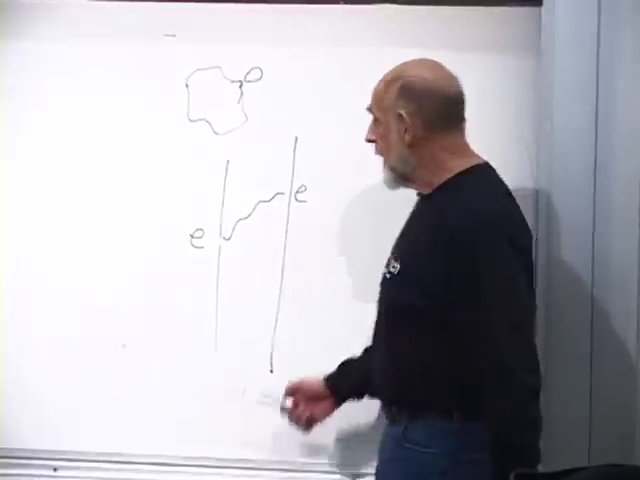
\includegraphics[width=0.72\textwidth]{lecture_06_figure_03.png}
\caption{黒板に描かれた完成した交換のスケッチ。結合定数が放出の際に、そして再び吸収の際に付随する。}
\lectureframe{00:11:30.000}
\end{figure}

弦理論版では光子をグラビトンに、電荷を\(g_s\)に置き換える。一つの因子が放出に伴い、もう一つが吸収に伴うので、重力の強さは\(g_s^2\)でスケールする。

長距離では、同じ相互作用がニュートンの力の法則を再現しなければならない。
\begin{equation}
F_{\mathrm{grav}}\sim G_N\frac{M_1M_2}{r^2}.
\end{equation}
質量と逆二乗依存性は源と伝播を記述する。ここで必要な点は、それらに掛かる結合定数である。

\begin{figure}[htbp]
\centering
\begin{tikzpicture}[x=1cm,y=1cm]
  \node[font=\small\bfseries] at (1.8,3.55) {electromagnetism};
  \draw[line width=0.8pt] (0,0) -- (0,3);
  \draw[line width=0.8pt] (3.6,0) -- (3.6,3);
  \draw[line width=0.8pt] plot[smooth] coordinates {(0,1.5) (0.45,1.72) (0.9,1.28) (1.35,1.72) (1.8,1.28) (2.25,1.72) (2.7,1.28) (3.15,1.72) (3.6,1.5)};
  \node[below] at (0,1.42) {\(e\)};
  \node[below] at (3.6,1.42) {\(e\)};
  \node[font=\small] at (1.8,0.25) {exchange strength \(\propto e^2\)};
  \node[font=\small\bfseries] at (7.2,3.55) {string gravity};
  \draw[line width=0.8pt,rounded corners=6pt] (5.4,0) -- (5.2,0.7) -- (5.5,1.5) -- (5.25,2.3) -- (5.4,3);
  \draw[line width=0.8pt,rounded corners=6pt] (9,0) -- (9.2,0.7) -- (8.9,1.5) -- (9.15,2.3) -- (9,3);
  \draw[line width=0.8pt] plot[smooth] coordinates {(5.5,1.5) (5.95,1.72) (6.4,1.28) (6.85,1.72) (7.3,1.28) (7.75,1.72) (8.2,1.28) (8.65,1.72) (8.9,1.5)};
  \node[below] at (5.5,1.42) {\(g_s\)};
  \node[below] at (8.9,1.42) {\(g_s\)};
  \node[font=\small] at (7.2,0.25) {exchange strength \(\propto g_s^2\)};
\end{tikzpicture}
\caption{結合の数え方の類推。交換される量子の各端が1つの相互作用因子を与える。}
\end{figure}

この観察はニュートン定数をほとんど決定する。結合定数\(g_s\)は無次元であり、一方、四次元では\(G_N\)は長さの二乗の次元をもつ。利用可能な微視的長さは\(\ell_s\)であるから、
\begin{equation}
G_N\sim g_s^2\ell_s^2.
\label{eq:l06-newton-string}
\end{equation}
これと式~\eqref{eq:l06-planck-area}を組み合わせると、
\begin{equation}
\ell_p\sim g_s\ell_s.
\label{eq:l06-planck-string}
\end{equation}

\begin{figure}[htbp]
\centering
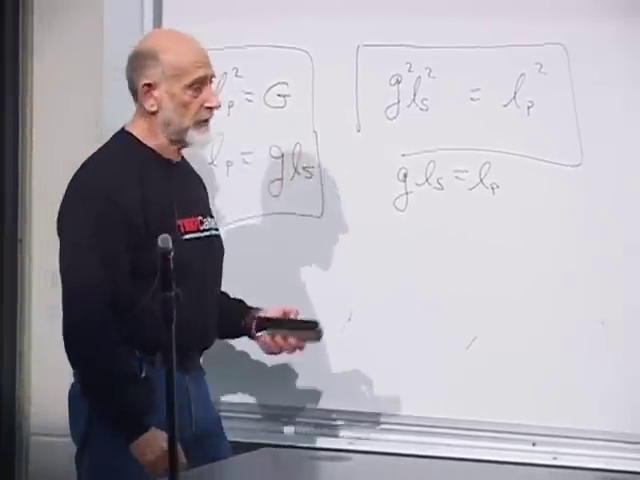
\includegraphics[width=0.72\textwidth]{lecture_06_figure_04.png}
\caption{黒板に残された基本関係式：\(\ell_p^2=G_N\)および\(\ell_p\sim g_s\ell_s\)。}
\lectureframe{00:15:45.000}
\end{figure}

式~\eqref{eq:l06-newton-string}はこの講義全体で用いられる簡略化された関係式である。\editorialnote{コンパクト化された弦理論では、有効4次元ニュートン定数はコンパクト化体積と1の程度の規約にも依存する。講義ではそれらのデータを抑え、対応関係のスケーリングを際立たせている。}

\begin{classroomqa}
\audiencequestion{\(g_s\)は1より大きいか小さいか、そしてどちらの長さがより大きいか。\lecturetimestamp{00:16:00}}
\lecturerresponse{我々は弱結合\(g_s<1\)で考える。すると\(\ell_p\sim g_s\ell_s\)は弦の長さがプランク長さより大きいことを意味する。強結合は別の記述を必要とし、ここでは不要である。}
\end{classroomqa}

\section{ブラックホールの数え上げ}

ボルツマン定数と数値因子を抑えると、ベッケンシュタイン--ホーキングエントロピーは
\begin{equation}
S_{\mathrm{BH}}=\frac{A}{4G_N}sim\frac{A}{G_N}sim\frac{A}{\ell_p^2}.
\label{eq:l06-bh-area}
\end{equation}
因子\(1/4\)は半古典的公式において厳密であるが、このスケーリングの議論では役割を果たさない。

\begin{classroomqa}
\audiencequestion{添字``BH''はブラックホールを意味するのか、それともベッケンシュタイン--ホーキングを意味するのか。\lecturetimestamp{00:16:51}}
\lecturerresponse{我々の目的には、両方を思い起こさせるものであればよい。重要なのは、エントロピーがプランク面積で測った事象の地平面の面積であるという点である。}
\end{classroomqa}

4次元シュヴァルツシルトブラックホールに対して、
\begin{equation}
R_s=2G_NM,
\qquad
A=4\pi R_s^2.
\end{equation}
講義でそうするように\(2\)と\(4\pi\)を落とすと、
\begin{align}
S_{\mathrm{BH}}
&\sim \frac{R_s^2}{G_N}
\sim \frac{(G_NM)^2}{G_N} \\
&\sim M^2G_N
\sim M^2\ell_p^2.
\label{eq:l06-bh-mass}
\end{align}
これが我々が弦の数え上げと比較する形である。

\section{長い弦のランダムウォークとしての描像}

小さな弦から始めて、それにエネルギーを注ぎ込む。一般の高度に励起された弦は整ったループのままではいない。それは、ひどく絡まったリールから出た釣り糸のように、長く絡み合った対象となる。巨視的に見て同じに見える配位が膨大に存在するため、この絡まりはエントロピーをもつ。

それらを数えるために、空間をリンクの長さが\(\ell_s\)である格子で置き換える。サイトは頂点、リンクは線分、基本正方形はプラケットである。弦はリンクの連結した列で表される。この模型は意図的に粗いものであるが、その指数的な状態数は望ましいスケーリングを捉えている。

\begin{figure}[htbp]
\centering
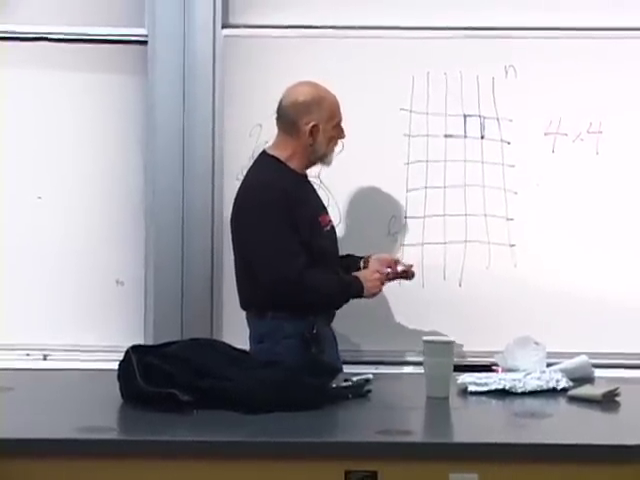
\includegraphics[width=0.72\textwidth]{lecture_06_figure_05.png}
\caption{2次元格子模型。青い線分は弦の1ステップを示し、各サイトで4つの可能な継続が数えられる。}
\lectureframe{00:23:50.000}
\end{figure}

\begin{classroomqa}
\audiencequestion{おもちゃのウォークの各ステップで何通りの選択肢があるか。\lecturetimestamp{00:22:43}}
\lecturerresponse{正方形格子上では4通りである。即座の後戻りが許されるからである。3次元では6通りになるであろう。別の格子ではその通常の数は変わるが、ウォークの数がリンクの数に対して指数的に増大するという事実は変わらない。}
\end{classroomqa}

弦が\(n\)個のリンクをもつなら、2次元のおもちゃの数え上げは
\begin{equation}
\Omega_n\sim4^n.
\label{eq:l06-walk-count}
\end{equation}
例外的な直線ウォークが1つあるが、それは\(4^n\)個のうちの1つの状態にすぎない。典型的なウォークは繰り返し折り畳まれ、絡まった球を占める。大きな\(n\)に対して、ランダムに生成されたほとんどすべての配位は定性的に他のすべてと同じに見える。

エントロピーは巨視的に区別できない配位の数の対数である：
\begin{equation}
S_{\mathrm{st}}=\log\Omega_n\sim n\log4\sim n.
\label{eq:l06-string-entropy-n}
\end{equation}

\begin{classroomqa}
\audiencequestion{なぜエントロピーは\(4^n\)ではなく\(n\)に比例するようになるのか。\lecturetimestamp{00:25:39}}
\lecturerresponse{エントロピーは状態数の対数である。したがって\(\log(4^n)=n\log4\)であり、因子\(\log4\)は1の程度の定数であり、我々はそれを抑える。}
\end{classroomqa}

\(L\)が弦を一端から他端までたどって得られる輪郭長であるなら、
\begin{equation}
n=\frac{L}{\ell_s},
\qquad
S_{\mathrm{st}}\sim\frac{L}{\ell_s}.
\label{eq:l06-string-entropy-length}
\end{equation}
ここで\(L\)は絡まった球の直径ではない。それは弦に沿って測ったはるかに長い距離である。

次に輪郭長を質量と交換する。\(c=\hbar=1\)のもとで、質量は逆長さの次元をもつ。したがって弦の大きさの1つのリンクは程度
\begin{equation}
m_{\mathrm{link}}\sim\frac{1}{\ell_s}.
\label{eq:l06-link-mass}
\end{equation}
の質量を担う

\begin{classroomqa}
\audiencequestion{なぜ1つのリンクの質量は\(1/\ell_s\)としてスケールしなければならないのか。\lecturetimestamp{00:29:20}}
\lecturerresponse{これらの単位では質量は逆長さであり、\(\ell_s\)が唯一利用可能な長さである。同等に、程度\(1/\ell_s^2\)の弦の張力にリンク長\(\ell_s\)を掛けると同じ結果を与える。}
\end{classroomqa}

すると完全な弦は
\begin{equation}
M\sim n m_{\mathrm{link}}
\sim\frac{n}{\ell_s}
\sim\frac{L}{\ell_s^2},
\qquad
L\sim M\ell_s^2.
\label{eq:l06-string-mass}
\end{equation}
となる。式~\eqref{eq:l06-string-entropy-length}に代入すると
\begin{equation}
S_{\mathrm{st}}\sim M\ell_s.
\label{eq:l06-string-entropy-mass}
\end{equation}
が得られる。格子ウォークは世界面の拘束条件と数値係数を無視しているが、高度に励起された弦スペクトルの指数的成長がこの同じ主要なスケーリングを与える。\editorialnote{このランダムウォーク構成は弦状態の高準位密度のための記憶術であり、基本弦の文字通りの離散化ではない。}

\section{議論の出発点となる不一致}

二つの答えは今や
\begin{equation}
S_{\mathrm{BH}}\sim M^2\ell_p^2,
\qquad
S_{\mathrm{st}}\sim M\ell_s.
\label{eq:l06-two-entropies}
\end{equation}
である。それらは互いに似ているが、固定された質量と任意の結合定数において等しくはない。ブラックホールの表式は\(M\)について二次であり、弦の表式は線形である。高温の弦が単にブラックホールであると宣言することはできない。二つの領域がどのように接続するかを説明しない限り。

\begin{figure}[htbp]
\centering
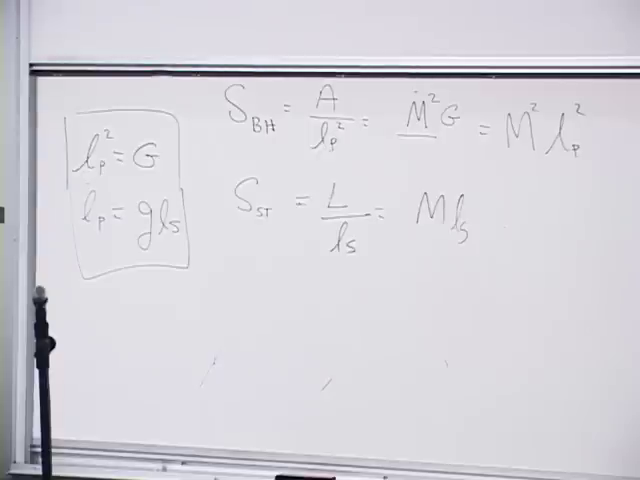
\includegraphics[width=0.78\textwidth]{lecture_06_figure_06.png}
\caption{妨げのないボード比較：上にブラックホールエントロピー、下に長い弦のエントロピー、左にプランク--弦関係を保持。}
\lectureframe{00:33:20.000}
\end{figure}

ここで講義は中断した。このサスペンスは有用である。不一致はアイデアの失敗ではなく、重力の強さを変えながら同じ状態を比較しなければならないという手がかりである。

\section{結合定数のつまみを回す}

\(\ell_s\)を固定し、\(g_s\)が変化しうると想像する。\(g_s=0\)では、弦は分裂も結合もせず、\(G_N\sim g_s^2\ell_s^2\)であるため重力は消える。十分にエネルギーの高い状態は、そのとき長く弱く相互作用する弦である。

\(g_s\)をゆっくり増加させる。弦の相互作用が可能になり、そして現在の議論にとってより重要なことに、重力が強くなる。

\begin{classroomqa}
\audiencequestion{\(g_s\)が増加するとき、最初の効果は単に弦がより短い弦に分裂することだろうか。\lecturetimestamp{00:36:29}}
\lecturerresponse{分裂と結合が可能になるが、\(\ell_s\)を固定し、高エントロピー状態を追跡する。中心的な効果は\(G_N\)が成長することであり、それゆえ長い弦の自己重力がもつれた球を内側に引き寄せる。}
\end{classroomqa}

物体は収縮し、より高密度になる。その重力ポテンシャルエネルギーは負であるため、収縮はその全エネルギーを低下させ、したがってその質量を低下させる。

\begin{classroomqa}
\audiencequestion{自己重力が弦を引き寄せるにつれて、エネルギーは増加するか減少するか。\lecturetimestamp{00:37:48}}
\lecturerresponse{減少する。結合エネルギーがより負になる。同じ状態を追跡し続けているにもかかわらず、経路上の質量は固定されている必要はない。}
\end{classroomqa}

最終的に物体の大きさはそのシュヴァルツシルト半径に匹敵する。その点を超えると、ブラックホールの記述が自然なものとなる。より大きな初期励起は、より小さな結合定数でこの条件に達する。なぜなら、より重い物体は地平線を形成するためにより少ない重力の強さを必要とするからである。

\begin{figure}[htbp]
\centering
\resizebox{0.95\linewidth}{!}{%
\begin{tikzpicture}[x=1cm,y=1cm,>=Latex]
  \draw[->,line width=0.9pt] (0,0) -- (11,0) node[right] {increasing \(g_s\)};
  \node[draw,rounded corners,align=center,minimum width=2.6cm,minimum height=1.15cm] at (1.8,1.5) {long excited string\\weak self-gravity};
  \node[draw,rounded corners,align=center,minimum width=2.6cm,minimum height=1.15cm] at (5.5,1.5) {correspondence point\\\(R_s\sim\ell_s\)};
  \node[draw,circle,align=center,minimum size=1.8cm] at (9.3,1.5) {black\\hole};
  \draw[->,line width=0.8pt] (3.15,1.5) -- (4.1,1.5) node[midway,above,font=\small] {contracts};
  \draw[->,line width=0.8pt] (6.9,1.5) -- (8.25,1.5);
  \node[font=\small,align=center] at (5.5,-0.65) {same family of states followed slowly;\\binding energy and mass may change};
\end{tikzpicture}
}
\caption{固定された\(\ell_s\)における対応の経路。矢印を逆にたどると、ブラックホール状態が長い弦の状態に戻る。}
\end{figure}

\begin{classroomqa}
\audiencequestion{\(g_s\)がゼロと1の間にあると想像すべきだろうか。\lecturetimestamp{00:40:18}}
\lecturerresponse{はい。議論は弱結合領域にとどまる。\(g_s\)が非常に小さければ、ブラックホールになる前に状態は相応に重くなければならない。制御が不十分な\(g_s>1\)領域に入る必要はない。}
\end{classroomqa}

この思考実験において、ゆっくりした変化は可逆である。

\begin{classroomqa}
\audiencequestion{重力がもはやブラックホールをまとめておけないところまで結合定数を再び下げると、それは何になるか。\lecturetimestamp{00:41:37}}
\lecturerresponse{長い弦である。重力が消えるとき、この構成のすべては弦状態で記述されなければならない。つまみを一方に回すと弦がブラックホールに写像され、逆に回すとブラックホールが弦に写像される。}
\end{classroomqa}

固定された全エネルギーと固定された体積の下で、支配的な高エントロピー配置は、膨大な数の短い弦ではなく、本質的に一つの長い弦である。この主張はここでは導出されない。それはハゲドルン領域近傍における弦の統計力学の結果であり、再び取り上げられるであろう。

\section{外部の観測者が見るもの}

物体がブラックホールとして記述されるとき、弦はどこにあるのか。外部の記述では、それは突然消えるのではない。シュヴァルツシルト時間は見かけの横断を任意に遅い時間へと送るので、弦的な自由度は地平線上またはその近くに蓄積するものとして表される。

\begin{figure}[htbp]
\centering
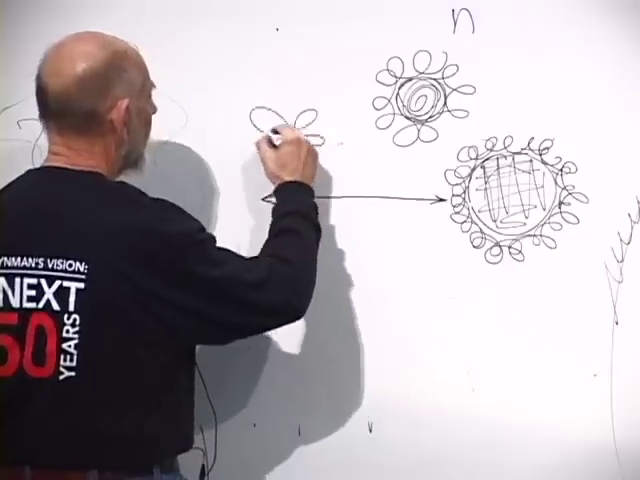
\includegraphics[width=0.72\textwidth]{lecture_06_figure_07.png}
\caption{巨視的な地平線——そこでは弦スケールの構造が薄い綿毛である——と、半径がループスケールに近づくより小さな地平線とのボード比較。}
\lectureframe{00:45:30.000}
\end{figure}

\(R_s\gg\ell_s\)では、ブラックホールは巨視的であり、弦スケールの構造は事象の地平面半径に対して薄い層にすぎない。半径が\(\ell_s\)に向かって減少するにつれて、滑らかなブラックホールと伸長した弦との区別は意味を失う。これは外部からの、引き伸ばされた地平面による記述であり、落下する物質が正則な地平面を決して横切らないという座標に依存しない主張と混同してはならない。\editorialnote{この講義では、ブラックホール相補性でよく知られた外部記述を用いる。``地平面上''という語句は、外部記述によって分解される自由度を指し、それらの共変的な位置を別途導出するものではない。}

クロスオーバーは次式のときに起こる。
\begin{equation}
R_s\sim\ell_s.
\label{eq:l06-correspondence-radius}
\end{equation}
弦スケール以下では、シュヴァルツシルト幾何はそれを支えるはずの構造を分解できない。ループは本来の地平面から揺らぎ離れ、その状態はむしろ弦と呼ぶのが適切である。

\section{対応点}

式~\eqref{eq:l06-correspondence-radius}において\(R_s\sim G_NM\)を用いる。
\begin{equation}
G_NM\sim\ell_s.
\end{equation}
次に\(G_N\sim g_s^2\ell_s^2\)を代入する。
\begin{equation}
M g_s^2\ell_s^2\sim\ell_s,
\qquad
M g_s^2\ell_s\sim1.
\label{eq:l06-correspondence-condition}
\end{equation}

\begin{figure}[htbp]
\centering
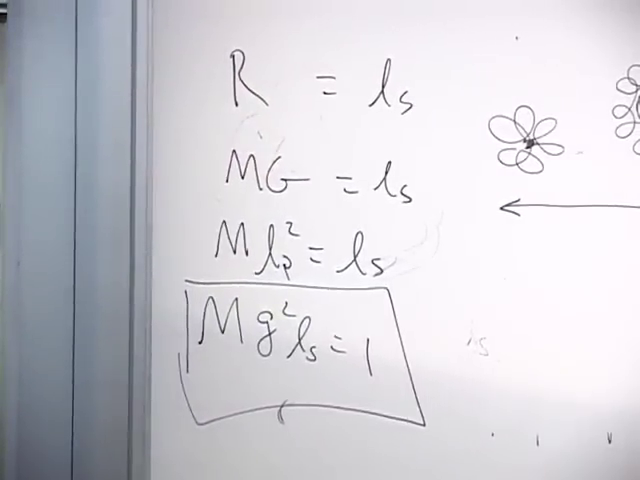
\includegraphics[width=0.72\textwidth]{lecture_06_figure_08.png}
\caption{黒板での完全な遷移の代数：\(R_s\sim\ell_s\)は枠で囲まれた無次元条件\(Mg_s^2\ell_s\sim1\)に至る。}
\lectureframe{00:49:50.000}
\end{figure}

聴衆の一人が、この条件が何を準備しているかに気づいた。対応点では、
\begin{align}
S_{\mathrm{BH}}
&\sim M^2\ell_p^2
\sim M^2g_s^2\ell_s^2 \\
&=(M\ell_s)(Mg_s^2\ell_s)
\sim M\ell_s
\sim S_{\mathrm{st}}.
\label{eq:l06-entropy-preview}
\end{align}

\begin{classroomqa}
\audiencequestion{これらの式はすでにブラックホールと弦のエントロピーが等しくなることを含意しているのか。\lecturetimestamp{00:50:18}}
\lecturerresponse{はい。まさにそこへ計算が向かっている。材料は黒板に置かれたが、講義は対応の論理を注意深く見直せるよう、それらの完全な組み立てを延期する。}
\end{classroomqa}

式~\eqref{eq:l06-entropy-preview}は、このやり取りに暗黙に含まれる一行の代数的予告である。それはスケーリングを確立するものであり、厳密な係数\(1/4\)ではない。厳密な微視的対応には、より制御されたブラックホールとより詳細な弦の構成が必要である。\editorialnote{講義は式~\eqref{eq:l06-entropy-preview}を完成した導出として提示する手前で止まっている。ここに書き出したのは、聴衆が明示的にこの等式を指摘し、必要な関係がすべてすでに現れているからである。}

\section{なぜエントロピーを持ち越せるのか}

論理的な材料がもう一つ残っている。磁場や\(g_s\)のような制御パラメータを、系が孤立し、その発展が可逆である間に十分ゆっくり変化させるとする。エネルギー、大きさ、束縛は変化しうるが、エントロピーは保存される。
\begin{equation}
\Delta S=0.
\label{eq:l06-adiabatic-entropy}
\end{equation}
講義はこれを情報の保存と結びつける。エントロピーは粗視化された記述によって隠された情報を測る。ハミルトニアンのゆっくりした可逆変化は、その情報を消すことなく状態を並べ替える。

\begin{classroomqa}
\audiencequestion{エントロピーが一定であるには、経路が相転移を避ける必要があるのか。\lecturetimestamp{00:54:01}}
\lecturerresponse{はい、状態を連続的に追跡できなければならない。有限系には無限体積の場合のような厳密に非解析的な熱力学的相転移はなく、変化が十分ゆっくりであれば、対応は滑らかなクロスオーバーとして扱える。}
\end{classroomqa}

ここで断熱とは、より強い準静的・可逆の意味で用いられている。断熱的だが不可逆な過程はエントロピーを生みうる。ゆっくりであることと状態を追跡できることが本質的である。\editorialnote{熱力学的な主張\(\Delta S=0\)には可逆な断熱経路が必要である。量子力学的には、対応する考え方は、制御されない準位遷移なしにパラメータが変化するにつれて同じ状態の集合を追跡することである。}

\begin{classroomqa}
\audiencequestion{同じ全質量を持つ複数の短い弦よりも、一つの長い弦の方がなぜエントロピーが大きいのか。\lecturetimestamp{00:54:44}}
\lecturerresponse{直感に反するが、高エネルギー状態の明示的な数え上げは、固定体積において長い弦の成分を有利にする。証明は後回しにする。現在の議論には、ブラックホールが非常に多くの短い弦の希薄な気体ではなく、最大エントロピーの弦のセクターに対応することだけが必要である。}
\end{classroomqa}

したがって操作的な戦略は次のとおりである。
\begin{enumerate}
\item 結合\(g_{s,0}\)において質量\(M_0\)のブラックホールから始める。
\item 同じ高エントロピー状態の族を追跡しながら\(g_s\)をゆっくり下げる。
\item ブラックホール記述が長い弦の記述になる\(R_s\sim\ell_s\)で止める。
\item \(S_{\mathrm{st}}\sim M\ell_s\)を用いて弦の状態を数える。
\item そのエントロピーを可逆経路に沿って元のブラックホールへ持ち戻す。
\end{enumerate}

\begin{figure}[htbp]
\centering
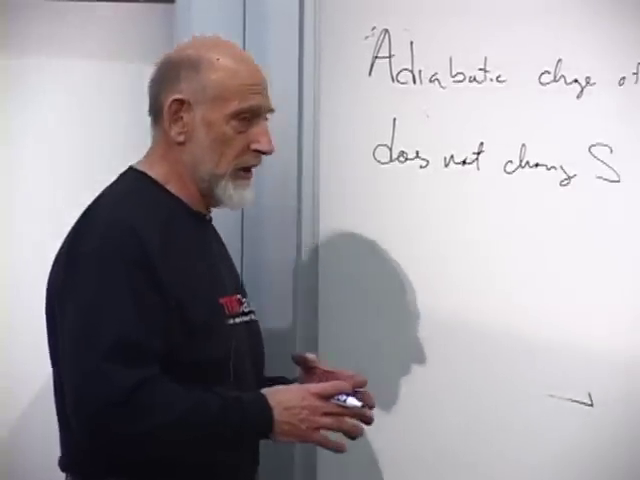
\includegraphics[width=0.72\textwidth]{lecture_06_figure_09.png}
\caption{戦略を述べる間、黒板に保たれる原理：\(g_s\)の断熱変化は\(S\)を変えない。}
\lectureframe{00:56:40.000}
\end{figure}

弦理論は、電荷をもつ回転する超対称な準極限および高次元ブラックホールに対して、はるかに精密なエントロピー数え上げを与えてきた。ここでの中性シュヴァルツシルトの議論は粗い対応関係の議論である。すなわち、状態密度のパラメトリックな振る舞いと物理的なクロスオーバーを同定するものであって、厳密に保護された縮退を与えるものではない。\editorialnote{厳密な一致が最も強いのは、結合定数が変化しても状態数が保護される特別なブラックホールに対してである。本講義では意図的に最も単純な桁程度の版を与えている。}

\begin{classroomqa}
\audiencequestion{重力を切ったとき、状態はちょうど1本ではなく2本の弦になりうるだろうか。\lecturetimestamp{00:58:25}}
\lecturerresponse{少数の長い弦に対しては有限の確率があり、1本ではなく2本を使っても主要なエントロピーのスケーリングは変わらない。議論を変えるのは、短い弦の巨大な気体への断片化である。高エネルギーでの統計的な数え上げはその結果を支持しない。}
\end{classroomqa}

ブラックホールはある領域に詰め込むことのできる最大のエントロピーであり、長い弦は重力を取り除いたときの対応する高エントロピー状態である。これら二つの記述は今や結びつけられているが、まだ精密計算へと展開されてはいない。次の段階は、代数を注意深く繰り返し、この対応がどこまで信頼できるかを問うことである。

\chapter{ブラックホールエントロピー、ホログラフィー、ド・ジッター空間}

\lectureoverview{前回の講義で始めた対応関係の議論を完成させる。強く励起された弦のエントロピーはその質量に比例し、シュヴァルツシルトブラックホールのエントロピーはその面積に比例する。二つの式は、強い重力を持つブラックホールを自由な弦と同一視することによってではなく、二つの記述が出会うまで弦結合定数をゆっくり変化させることによって結びつけられる。面積則はそこから自然にホログラフィー原理へと導き、講義の最後の部分では膨張する空間と、次にその地平線を調べることになるド・ジッター幾何学を導入する。}

\section{数え上げの問題に戻る}

長い弦の数え上げには未解決の点が一つあった。固定された全長がいくつかの弦に分割される場合、同じ長さの同一の弦は区別できない。それでも箱の中のそれらの位置は状態の一部であり、箱は対応する単一の長い弦が占めるのとほぼ同じ大きさに選ばれる。

\begin{classroomqa}
\audiencequestion{短い弦は互いに区別されるのか、またそれらの位置は数えられるのか。\lecturetimestamp{00:00:37}}
\lecturerresponse{同一の性質を持つ弦は区別できないが、箱の中のそれらの位置は数えられる。比較は固定された体積で行われ、長い弦が占める領域に合わせて選ばれる。}
\end{classroomqa}

それが片づいたので、目標を述べることができる。短い式のリストをまとめ、それらを用いてブラックホールエントロピーのスケーリングを導く。積分も無限和も必要ない。困難は代数的なものではなく、どの量をどの段階で比較してよいかを知ることにある。

\section{自然単位とプランク面積}

次のように置く。
\begin{equation}
c=\hbar=1,
\label{eq:l07-natural-units}
\end{equation}
ただしニュートン定数はあらわに残す。最初の帰結は、時間と長さが同じ単位を持つことである。光子の関係式
\begin{equation}
E=\frac{\hbar c}{\lambda}
\end{equation}
と質量とエネルギーの関係式\(E=mc^2\)から
\begin{equation}
[M]=L^{-1}.
\label{eq:l07-mass-dimension}
\end{equation}
が従う。したがって質量は逆長さとして表すことができる。

\begin{figure}[htbp]
\centering
\includegraphics[width=0.62\textwidth]{lecture_07_figure_02.png}
\caption{次元解析の冒頭における自然単位の規約。エネルギー公式は上の式で完成する。}
\lectureframe{00:03:27.900}
\end{figure}

\(G_N\)の単位を決めるには、ニュートン加速度を次元の帳尻合わせとしてのみ用いる。
\begin{equation}
a\sim\frac{G_NM}{R^2}.
\end{equation}
\(T\)と\(L\)は同じ単位を持つので、\([a]=L/T^2=L^{-1}\)である。式~\eqref{eq:l07-mass-dimension}と合わせて
\begin{equation}
[G_N]=L^2.
\end{equation}
が得られる。ニュートン定数はこれらの単位では面積である。プランク長を
\begin{equation}
G_N=\ell_p^2,
\label{eq:l07-planck-area}
\end{equation}
で定義すれば、\(A/G_N=A/\ell_p^2\)が無次元である理由は直ちに理解できる。すなわちプランク面積の単位で面積を測っているのである。

\section{弦結合定数と重力の強さ}

重力を今度は弦の言葉に翻訳しなければならない。有用な描像は交換過程である。弦が自分自身と交差すると、分裂して再結合することがある。小さな閉弦ループが一方の物体から放出され他方に吸収されることがあり、その励起が重力子であるとき、この過程が重力を媒介する。放出で一つの相互作用因子が現れ、吸収でもう一つ現れるので、交換の強さには\(g_s^2\)が含まれる。

結合定数\(g_s\)は無次元である。より正確には、それは振幅レベルの結合定数であり、確率や率は\(g_s^2\)の次数から始まる。\editorialnote{講義では時に\(g_s\)を確率と呼び、それを確率の平方根と訂正する。摂動的な結合定数は振幅レベルに属する。} \(G_N\)は面積の次元を持つので、依然として長さのスケールが欠けている。基本弦の長さ\(\ell_s\)、すなわち一つの素的な弦の揺れのスケールがそれを与える。
\begin{equation}
G_N\sim g_s^2\ell_s^2,
\qquad
\ell_p\sim g_s\ell_s.
\label{eq:l07-planck-string}
\end{equation}

\begin{figure}[htbp]
\centering
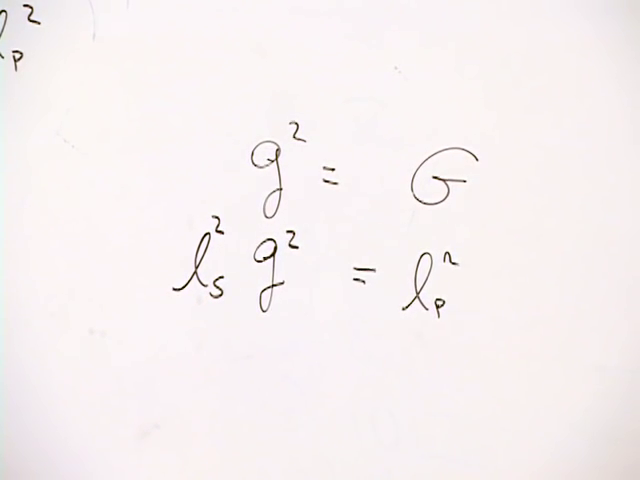
\includegraphics[width=0.72\textwidth]{lecture_07_figure_05.png}
\caption{黒板に書かれた結合定数の関係: \(G_N=\ell_p^2\)および\(g_s^2\ell_s^2\sim\ell_p^2\)。}
\lectureframe{00:12:15.000}
\end{figure}

弱結合\(g_s\ll1\)では、プランク長は弦の長さよりずっと小さい。\(g_s\)を小さくすると、素的な弦のスケールを固定したまま重力が弱くなる。\editorialnote{有効四次元理論では、コンパクト化のデータと数値的な規約も\(G_N\)に入ってくる。それらはこのスケーリングの議論では固定され、抑えられている。}

\section{長い弦の数え上げ}

エントロピーは、状態を指定するのに必要な素的な決定の数を数える。強く励起された弦を正方形格子上の歩みに置き換える。各頂点で次の辺は四つの方向のいずれかを向きうる。素的な選択を一つの四択の決定として記述するか二つの二択の決定として記述するかは、一次の定数を変えるだけである。重要なのは歩数の数である。

\(L\) が弦の輪郭長であり、各ステップの長さが \(\ell_s\) であるならば、
\begin{equation}
N=\frac{L}{\ell_s}
\end{equation}
ステップが必要である。ウォークの数は指数的に増大し、模式的には \(\Omega_N\sim q^N\) で、\(q\) は1の程度であり、したがって
\begin{equation}
S_{\mathrm{str}}=\log\Omega_N\sim N\sim\frac{L}{\ell_s}.
\label{eq:l07-string-entropy-length}
\end{equation}

\begin{figure}[htbp]
\centering
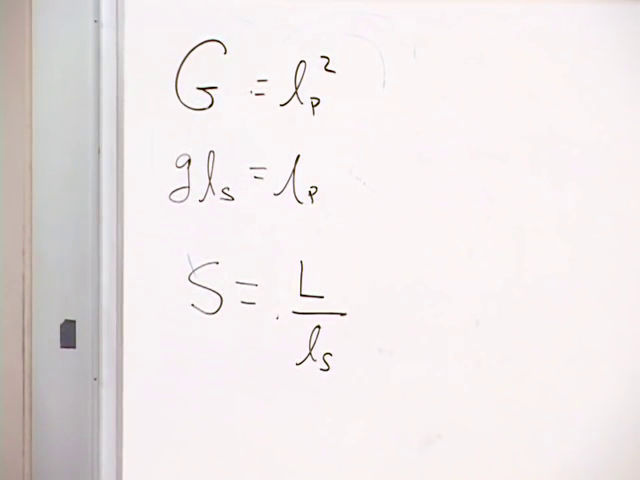
\includegraphics[width=0.68\textwidth]{lecture_07_figure_03.png}

\vspace{0.7em}
\begin{tikzpicture}[scale=0.82]
  \draw[step=0.8cm,gray!45,thin] (0,0) grid (6.4,4.0);
  \draw[very thick,blue!60!black]
    (0.8,0.8)--(1.6,0.8)--(1.6,1.6)--(2.4,1.6)--(2.4,2.4)--
    (3.2,2.4)--(3.2,1.6)--(4.0,1.6)--(4.0,2.4)--(4.8,2.4)--
    (4.8,3.2)--(5.6,3.2);
  \draw[<->,thick] (0.8,-0.35)--(1.6,-0.35);
  \node[below] at (1.2,-0.35) {step \(\ell_s\)};
  \node[align=center] at (8.1,2.0) {\(N=L/\ell_s\) steps\\[0.3em]\(S_{\mathrm{str}}\sim N\)};
\end{tikzpicture}
\caption{黒板上の格子模型とその整理されたランダムウォーク解釈。選択肢の数を決めるのは、もつれた球の直径ではなく輪郭長である。}
\lectureframe{00:17:20.000}
\end{figure}

質量は同じ基本セグメントから数えられる。長さ \(\ell_s\) のセグメントは質量スケール
\begin{equation}
m_{\mathrm{seg}}\sim\frac{1}{\ell_s}.
\end{equation} をもつ

\begin{classroomqa}
\audiencequestion{基本セグメントに長さ \(\ell_s\) が割り当てられているのか。\lecturetimestamp{00:18:56}}
\lecturerresponse{はい。その特徴的長さは \(\ell_s\) であるので、自然単位ではその特徴的質量は \(1/\ell_s\) である。}
\end{classroomqa}

\(L/\ell_s\) 個のセグメント質量を加えると
\begin{equation}
M\sim\frac{L}{\ell_s}\frac{1}{\ell_s}
=\frac{L}{\ell_s^2},
\qquad
L\sim M\ell_s^2.
\label{eq:l07-string-mass}
\end{equation}
振動する弦の運動エネルギーとポテンシャルエネルギーはこのスケーリング関係に圧縮されている。詳細な統計力学的取り扱いでも同じ依存性が得られる。式~\eqref{eq:l07-string-entropy-length}に代入すると、我々が必要とする弦の公式が得られる：
\begin{equation}
S_{\mathrm{str}}\sim M\ell_s.
\label{eq:l07-string-entropy-mass}
\end{equation}

\begin{figure}[htbp]
\centering
\includegraphics[width=0.66\textwidth]{lecture_07_figure_04.png}
\caption{比較の前にまとめられた弦側の列：\(\ell_p\sim g_s\ell_s\)、\(S_{\mathrm{str}}\sim L/\ell_s\sim M\ell_s\)、および \(M\sim L/\ell_s^2\)。}
\lectureframe{00:21:57.800}
\end{figure}

\section{なぜ自由弦はまだブラックホールではないのか}

重力側では、厳密な半古典的公式は
\begin{equation}
S_{\mathrm{BH}}=\frac{A}{4G_N}.
\label{eq:l07-bh-exact}
\end{equation} である

\begin{classroomqa}
\audiencequestion{分母に入る数値係数は何か。\lecturetimestamp{00:23:28}}
\lecturerresponse{4。対応関係の議論はスケーリングを再現するが、その厳密な因子を決定するには粗すぎる。}
\end{classroomqa}

4次元シュヴァルツシルトブラックホールに対して、
\begin{equation}
R_s=2G_NM,
\qquad
A=4\pi R_s^2.
\end{equation}
講義で行ったように数値定数を落とすと、
\begin{align}
S_{\mathrm{BH}}
&\sim\frac{A}{G_N}
\sim\frac{(G_NM)^2}{G_N} \\
&\sim M^2G_N
\sim M^2\ell_p^2.
\label{eq:l07-bh-scaling}
\end{align}

\begin{figure}[htbp]
\centering
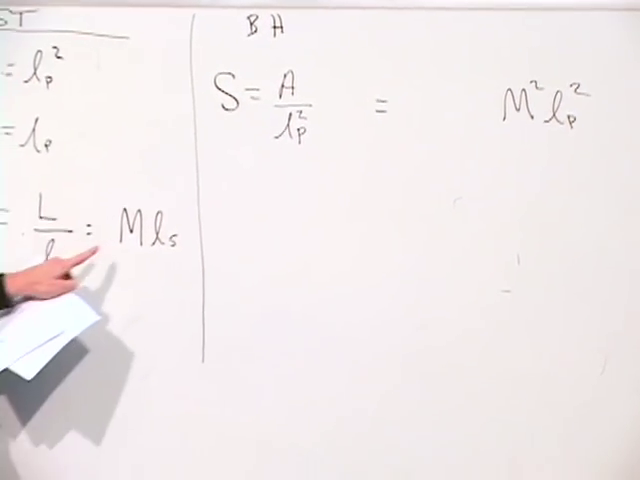
\includegraphics[width=0.72\textwidth]{lecture_07_figure_06.png}
\caption{黒板上で完成した比較：弦のエントロピーは弦単位での長さであるのに対し、ブラックホールのエントロピーはプランク単位での面積である。}
\lectureframe{00:25:35.000}
\end{figure}

式~\eqref{eq:l07-string-entropy-mass}と式\eqref{eq:l07-bh-scaling}の類似は示唆的であるが、それらは同じ公式ではない。元のブラックホールを単に自由弦と呼んで代入するのは誤りであろう。自由弦の数え上げは弦の部分間の引力相互作用を省略しており、まさにその相互作用が弦をブラックホールへと圧縮し、負の結合エネルギーを通じてその全エネルギーを下げるのである。

恒星はこの誤りを身近なものにする。恒星質量の高温ガスを大きすぎる箱に入れたものは、同じ温度であっても恒星の模型ではない。自己重力が平衡サイズとエネルギー・エントロピー関係を変える。長い弦のあらゆる自己相互作用を追跡するのは困難であろうから、我々はそうすることを避ける。

\begin{classroomqa}
\audiencequestion{小さなループが長い弦から離れると、そのエントロピーは減少する。では重力子の交換は重力系のエントロピーを下げるのか。\lecturetimestamp{00:28:48}}
\lecturerresponse{ここで用いている平衡交換過程ではそうではない。仮想励起は両方向に放出・吸収される。この絵は永続的な弦の断片の文字通りの損失ではない。その現在の唯一の目的は、2つの結合因子、したがって \(g_s^2\) 依存性を確立することである。}
\end{classroomqa}

\section{断熱対応ゲーム}

代わりに重力が無視できるところから始めよう。\(g_s\to0\) では、弦は分裂も結合もせずに交差し、自己重力引力は消える。\(\ell_s\) を固定したまま \(g_s\) を増加させる：重力が強まり、高度に励起された弦は収縮し、最終的にブラックホールになる。ダイヤルをゆっくり逆に回すと、ブラックホールは弦状態に戻らなければならない。それは少数の長い弦になるかもしれないが、前回の講義の高エネルギー数え上げによれば、支配的なセクターは短い弦の巨大なガスではなく1本の長い弦を含む。

\begin{classroomqa}
\audiencequestion{結合が変化する間、何が固定されているのか。\lecturetimestamp{00:32:19}}
\lecturerresponse{弦の長さ \(\ell_s\)、したがって基本弦質量スケール \(1/\ell_s\) が固定されている。ダイヤルは \(g_s\) を変え、それゆえ \(G_N\sim g_s^2\ell_s^2\) を変える。}
\end{classroomqa}

変化は遅く、孤立しており、可逆でなければならない。そのような条件下でエントロピーは断熱不変量である：
\begin{equation}
\Delta S=0.
\label{eq:l07-adiabatic}
\end{equation}
散逸的または制御されていない遷移が起こるならば、遅いだけでは十分ではない。ここで ``断熱'' とは、同じ状態の族を連続的に追跡できることを意味する。\editorialnote{これは断熱の可逆熱力学的な意味である。不可逆過程は熱流なしの意味で断熱的でありながら、なおエントロピーを生成しうる。}

対象とするブラックホールの質量を\(M_0\)、結合を\(g_{s,0}\)とする。これから説明しようとしている面積公式を使う前に、次元解析が言えるのは、中性で回転していないブラックホールのエントロピーは無次元の組み合わせ
\begin{equation}
S_{\mathrm{BH}}=f(M\ell_p)
=f(Mg_s\ell_s).
\label{eq:l07-entropy-function}
\end{equation}
のある関数であるということだけである。\(\ell_s\)を固定すると、等エントロピー経路はしたがって
\begin{equation}
Mg_s=M_0g_{s,0}
\label{eq:l07-adiabat}
\end{equation}
を一定に保つ。ただし、同じ状態の枝に沿って進む場合に限る。

\(g_s\)が減少するにつれて、負の結合エネルギーが取り除かれるので、この経路に沿って質量\(M\)は増大する。背後にある弦の配位もより強く束縛されなくなり、広がっていく。しかし、形式的なシュヴァルツシルト半径は断熱経路上で\(R_s\sim Mg_s^2\ell_s^2\sim g_s\ell_s\)のように振る舞うため、減少する。\editorialnote{口頭の議論では、重力結合から解放された物体について``grows''という表現が使われている。これは、導出された断熱経路に沿ってシュヴァルツシルト半径が増大するという意味に読んではならない。}

\begin{classroomqa}
\audiencequestion{重力が弱められると、この物体は成長するのか、それとも縮むのか。\lecturetimestamp{00:36:28}}
\lecturerresponse{その弦構造は解放されて膨張する一方、負の結合エネルギーが取り除かれるため質量は増大する。ブラックホールの公式が割り当てる半径は、弦のスケールに達するまで減少し、そこではそのブラックホール的記述はもはや有用でなくなる。}
\end{classroomqa}

\section{二つの曲線とその交点}

質量を縦軸に、弦結合を横軸にとる。式~\eqref{eq:l07-adiabat}は双曲線であり、\(M\propto g_s^{-1}\)である。

\begin{classroomqa}
\audiencequestion{積\(Mg_s\)が一定であるような曲線は何か。\lecturetimestamp{00:44:08}}
\lecturerresponse{双曲線である。それは目標点\((g_{s,0},M_0)\)を通る断熱経路である。}
\end{classroomqa}

第二の曲線は、二つの記述の間のクロスオーバーを表す。ブラックホールは、その半径が素弦の揺らぎより小さくなると、通常のシュヴァルツシルト幾何として解像できなくなる。したがって、対応点を
\begin{equation}
R_s\sim\ell_s.
\label{eq:l07-correspondence-radius}
\end{equation}
によって見積もる。\(R_s\sim MG_N\)と式~\eqref{eq:l07-planck-string}を用いると、これは
\begin{equation}
Mg_s^2\ell_s^2\sim\ell_s,
\qquad
Mg_s^2\sim\frac{1}{\ell_s}.
\label{eq:l07-transition-curve}
\end{equation}
となる。したがって、転移曲線は\(M\propto g_s^{-2}\)として減少し、断熱経路よりも急である。

\begin{figure}[htbp]
\centering
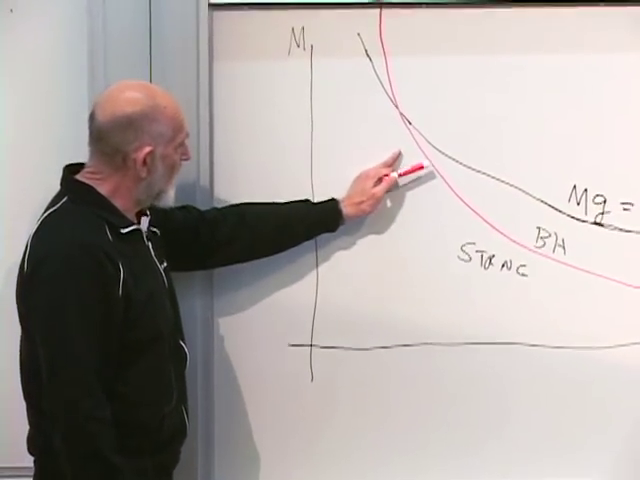
\includegraphics[width=0.70\textwidth]{lecture_07_figure_07.png}

\vspace{0.6em}
\begin{tikzpicture}[x=1cm,y=0.78cm]
  \draw[->] (0.4,0.4)--(7.0,0.4) node[right] {\(g_s\)};
  \draw[->] (0.4,0.4)--(0.4,6.5) node[above] {\(M\)};
  \draw[thick,black] plot[smooth] coordinates {(1.0,5.6) (1.5,4.0) (2.2,2.9) (3.2,2.1) (4.6,1.55) (6.3,1.2)};
  \draw[very thick,red!70!black] plot[smooth] coordinates {(1.25,6.0) (1.55,4.55) (2.0,3.15) (2.7,2.0) (3.8,1.25) (5.8,0.78)};
  \fill (2.05,3.1) circle (2pt) node[above right] {\((g_{s,*},M_*)\)};
  \node[black,rotate=-17] at (4.75,1.9) {\(Mg_s=M_0g_{s,0}\)};
  \node[red!70!black,rotate=-25] at (4.45,0.95) {\(Mg_s^2=1/\ell_s\)};
  \node at (5.75,3.5) {black hole};
  \node at (1.15,1.25) {string};
\end{tikzpicture}
\caption{黒板のグラフとその整理された解釈。黒い断熱経路は、物体が弦的になる点で、より急な赤い対応曲線と交わる。}
\lectureframe{00:49:35.000}
\end{figure}

交点\((M_*,g_{s,*})\)において、二つの方程式は
\begin{align}
M_*g_{s,*} &= M_0g_{s,0}, \\
M_*g_{s,*}^2 &\sim \frac{1}{\ell_s}.
\end{align}
である。第一の式を二乗し、第二の式で割ると、
\begin{equation}
M_*
\sim M_0^2g_{s,0}^2\ell_s.
\end{equation}
となる。\(\ell_s\)を掛けると、
\begin{equation}
M_*\ell_s
\sim M_0^2g_{s,0}^2\ell_s^2
\sim M_0^2G_{N,0}.
\label{eq:l07-crossover-result}
\end{equation}

\begin{figure}[htbp]
\centering
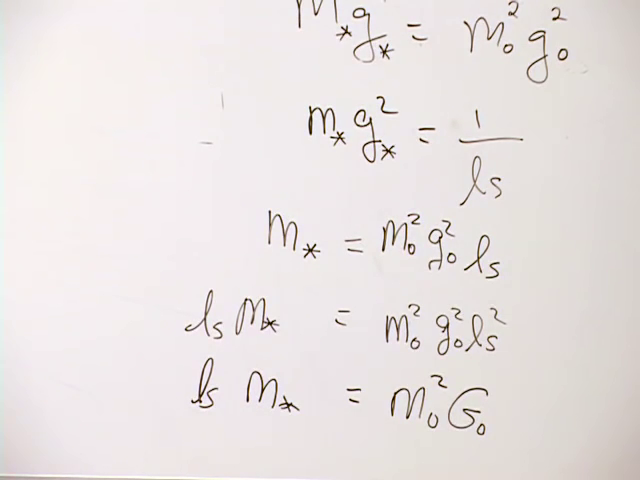
\includegraphics[width=0.68\textwidth]{lecture_07_figure_08.png}
\caption{\(M_*\ell_s=M_0^2g_{s,0}^2\ell_s^2=M_0^2G_{N,0}\)を含む、完成したクロスオーバー代数。}
\lectureframe{00:54:40.000}
\end{figure}

\begin{classroomqa}
\audiencequestion{二つの曲線の方程式を割ると、\(\ell_s\)は分子に来るべきか、それとも分母に来るべきか。\lecturetimestamp{00:52:41}}
\lecturerresponse{分子に来る。\(1/\ell_s\)で割ることは\(\ell_s\)を掛けることであり、そのため\(M_*\sim M_0^2g_{s,0}^2\ell_s\)となる。}
\end{classroomqa}

クロスオーバーでは弦の公式が有効なので、
\begin{equation}
S_*\sim M_*\ell_s.
\end{equation}
である。経路に沿ってエントロピーは変化しなかった。この主張を式~\eqref{eq:l07-crossover-result}と組み合わせると、元の対象ブラックホールのエントロピーが得られる：
\begin{equation}
S_{\mathrm{BH}}(M_0)
\sim M_0^2G_{N,0}
\sim M_0^2\ell_{p,0}^2.
\label{eq:l07-final-correspondence}
\end{equation}
これが求める面積則のスケーリングである。

\section{対応関係が証明することと証明しないこと}

この構成は、元の強い重力を持つブラックホールが自由な弦であるとは述べていない。物体を弦の数え上げが信頼できる領域へ移し、そこでエントロピーを読み取り、そのエントロピーを可逆な経路に沿って元へ運び戻すのである。転移は鋭く位置づけられた相境界ではなくクロスオーバーであるため、この見積もりでは式~\eqref{eq:l07-bh-exact}の係数\(1/4\)を決定することはできない。

それでも同じ論理は、荷電ブラックホール、他の次元のブラック物体、および拡張されたブラックブレーンに対してパラメトリックに機能する。より対称性が高く超対称な例では、結合が変化しても厳密な情報を保つ保護された状態の数え上げが可能である。それらの方法は数値係数を回復するが、現在の概念的議論には不要な数学的装置を追加する。

最も重要なのは、この計算が微視的解釈を与えることである。エントロピーは隠れた構造の証拠である。流体力学は分子を省いて密度、圧力、流れを記述するが、流体のエントロピーはそのような微視的自由度が存在することを明らかにする。一般相対性理論も同様に、その微視的状態を明示することなく事象の地平面を記述する。弦の数え上げは、重力の整合的な量子論がブラックホールのエントロピーを説明するのに十分な状態を含みうることを示している。

\begin{classroomqa}
\audiencequestion{二次の結果の代わりに\(S\sim M^3\ell_p^3\)だったなら、何を意味しただろうか。\lecturetimestamp{00:59:41}}
\lecturerresponse{それは体積則のように見えたであろう。部屋の中の普通の物質や一杯のコーヒーは体積に比例するエントロピーを持つ。二次の答えが特別なのは、\(R_s\sim M\ell_p^2\)を通じて、それが地平面の面積に比例するからである。}
\end{classroomqa}

この結果は、ベッケンシュタイン--ホーキングエントロピーが単なる形式的な熱力学的類推ではないことの証拠である。それは微視的な重力自由度を示唆している。ただし、初等的な導出はそれらの自由度を一つ一つ可視化するものではない。

\section{最大エントロピーからホログラフィーへ}

ここで問いを変える。指定された状態のエントロピーを問う代わりに、ある領域と両立する最大のエントロピーを問う。

部屋の通常の格子模型から始める。体積を大きさ\(V_{\mathrm{cell}}\)のセルに分割し、各セルに一つのイエス・ノーの問いを持たせる。すなわち占有か空かである。ススキンドは想像上の原子に、意図的にばかげた名前``meatonium''を与える。現実的な原子の詳細が数え上げの妨げにならないようにするためである。もし
\begin{equation}
N=\frac{V}{V_{\mathrm{cell}}},
\end{equation}
ならば、配位の数と最大エントロピーは
\begin{equation}
\Omega=2^N,
\qquad
S_{\max}=\log\Omega=N\log2
\sim\frac{V}{V_{\mathrm{cell}}}.
\label{eq:l07-volume-count}
\end{equation}

\begin{figure}[htbp]
\centering
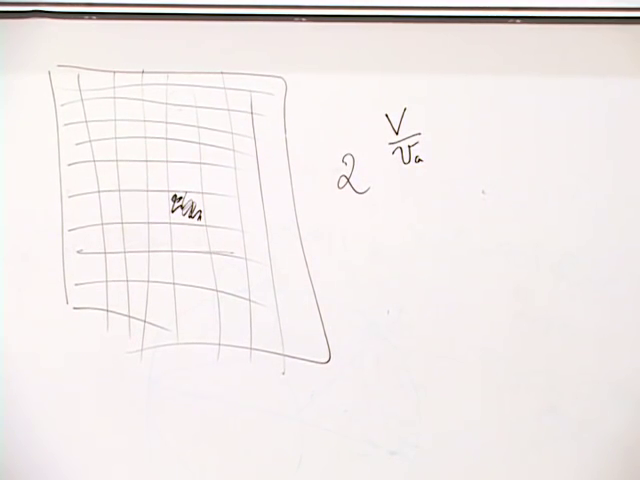
\includegraphics[width=0.68\textwidth]{lecture_07_figure_09.png}
\caption{セルに分割された部屋。各セルは二つの状態を持つ。これは最大エントロピーを数えており、授業が占める整然とした部屋のエントロピーではない。}
\lectureframe{01:05:20.000}
\end{figure}

実際の部屋はこの最大値よりはるかに低い。それらすべてのセルの選択を混沌と探索する状態は極めて高温であろう。おもちゃの模型から生き残るのは、独立な自由度の数、したがって最大エントロピーが体積に比例するという通常の期待である。

重力はその期待を覆す。境界面積\(A\)、初期エントロピー\(S_{\mathrm{i}}\)、質量\(M\)を持ち、その球をちょうど満たすブラックホールの質量\(M_{\mathrm{BH}}\)より小さい球状領域を考える。もし\(M\)がより大きければ、その事象の地平面はすでに選んだ境界を越えて広がっているであろう。

次に質量\(M_{\mathrm{BH}}-M\)の殻を送り込む。その組成は無関係である。講義は光、通常の物質、あるいはスイスチーズさえも許容する。それが崩壊するように整える。最終状態は、地平面がちょうどその領域を満たすブラックホールであり、エントロピーは
\begin{equation}
S_{\mathrm{f}}=\frac{A}{4G_N}.
\end{equation}
第二法則は次を要求する
\begin{equation}
S_{\mathrm{i}}\le S_{\mathrm{f}}
=\frac{A}{4G_N}.
\label{eq:l07-holographic-bound}
\end{equation}

\begin{figure}[htbp]
\centering
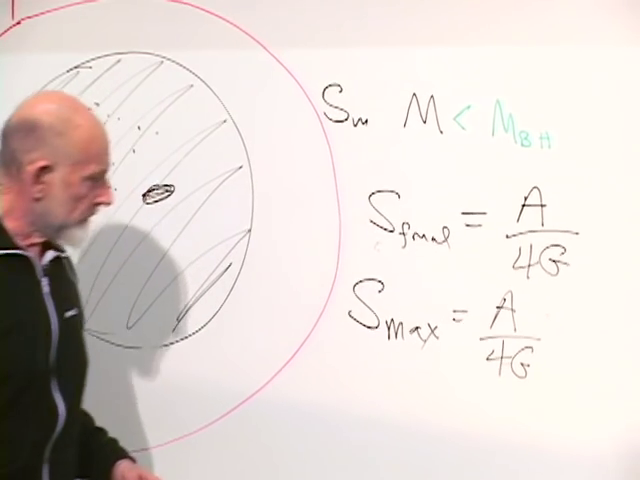
\includegraphics[width=0.70\textwidth]{lecture_07_figure_10.png}

\vspace{0.5em}
\begin{tikzpicture}[scale=0.88]
  \draw[thick] (0,0) circle (1.35);
  \draw[very thick,red!70!black] (0,0) circle (2.05);
  \fill[gray!25] (0,0) circle (1.32);
  \node at (0,0) {\(M,S_{\mathrm{i}}\)};
  \draw[-{Latex[length=3mm]},thick,red!70!black] (3.5,0)--(2.15,0);
  \node[align=center,right] at (3.5,0) {incoming shell\\\(M_{\mathrm{BH}}-M\)};
  \node[below] at (0,-2.2) {final horizon area \(A\)};
\end{tikzpicture}
\caption{殻の構成。選ばれた領域をちょうど満たす地平面を持つブラックホールを形成するのに十分な追加質量が内側へ送り込まれる。}
\lectureframe{01:13:30.000}
\end{figure}

その大きさのブラックホールは許される状態であり、不等式を飽和させるので、最大エントロピーは
\begin{equation}
S_{\max}=\frac{A}{4G_N}.
\label{eq:l07-holographic-maximum}
\end{equation}
これが数え上げの形でのホログラフィー原理である。重力のある領域における独立な自由度の最大数は、内部のプランク体積の数ではなく、その境界の面積に比例し、およそプランク面積あたり1桁程度の自由度である。\editorialnote{殻の議論は、その領域が述べられた方法で囲まれ崩壊できることを仮定している。より一般的な時空には共変的エントロピー境界が必要であるが、球対称の議論は講義で用いられた原理を捉えている。}

その隔たりは莫大である。局所場の理論の直観は、異なる内部点でなされた選択が独立に結合し、体積則を生み出すことを示唆する。重力は、そのような選択が十分に多ければそれ自体が崩壊し、ブラックホールがより大きな許容エントロピーを与えると言う。したがって境界の数え上げは体積の数え上げに対する小さな補正ではなく、ヒルベルト空間の異なる組織化である。

\begin{classroomqa}
\audiencequestion{ほぼ一様な密度を持つ非常に大きな宇宙では何が起こるか。\lecturetimestamp{01:15:48}}
\lecturerresponse{その問いは静的で球対称な構成ではなく宇宙論を必要とする。それはアインシュタイン方程式の膨張解への即座の移行を動機づける。}
\end{classroomqa}

\begin{classroomqa}
\audiencequestion{面積の境界は不確定性原理と関係しているか。\lecturetimestamp{01:16:03}}
\lecturerresponse{講義はこの問いを未解決のまま残し、次に宇宙論へ移る。}
\end{classroomqa}

\section{膨張する空間}

ここではアインシュタイン方程式から宇宙論的解を導出しない。解を書き下し、その読み方を学ぶ。空間的スライスは正に曲がって閉じているか、負に曲がって双曲的であるか、平坦でありうる。当面の議論では、時間依存の時空における空間的に平坦なユークリッド的スライスを取る。

\begin{classroomqa}
\audiencequestion{通常のユークリッド空間の時空版は何か。\lecturetimestamp{01:19:37}}
\lecturerresponse{ミンコフスキー空間である。ここで考える宇宙論は平坦な空間的スライスを持つが、その空間計量が時間とともに変化するため、ミンコフスキー時空ではない。}
\end{classroomqa}

おなじみの風船の描像は、1次元低い閉じた膨張面を表している。Susskindは、大きな印を付けた風船で実演を試みたことを回想している。マーカーがゴムを弱め、文字通りパンという音が生じた。この失敗は、この類推における概念的欠陥も露呈させる。普通の風船が膨張すると、そのゴム分子は離れていき、材料は薄くなってついには破れる。宇宙論的な空間は、薄められた局所的法則を獲得するわけではない。類推を保つには、新たなゴム分子を絶えず挿入し、あらゆる小さなパッチが同じ局所的性質を保つように想像しなければならない。平坦な模型では、風船を、一様に外側へ引っ張られ同様に補充される大きなシートに置き換える。

数学的には、膨張は計量に属する：
\begin{equation}
\begin{aligned}
ds^2&=-dt^2+a(t)^2d\mathbf{x}^2,\\
d\mathbf{x}^2&=\delta_{ij}\,dx^i dx^j
=dx^2+dy^2+dz^2.
\end{aligned}
\label{eq:l07-frw-metric}
\end{equation}

\begin{figure}[htbp]
\centering
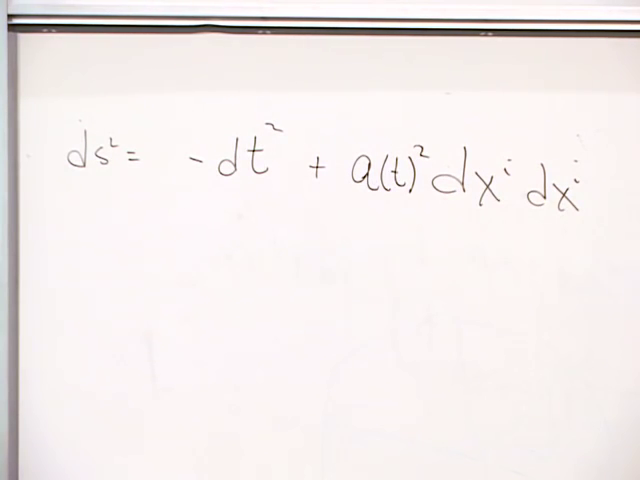
\includegraphics[width=0.72\textwidth]{lecture_07_figure_11.png}
\caption{黒板に書かれた、そのままの空間的に平坦な膨張計量。}
\lectureframe{01:25:10.000}
\end{figure}

固定された空間座標を保つ点は共動と呼ばれる。そのような2点が座標間隔\(\Delta x\)を持つとき、時刻\(t\)におけるそれらの固有距離は
\begin{equation}
D(t)=a(t)\Delta x.
\label{eq:l07-proper-distance}
\end{equation}
である。それらの座標は動かないが、それらの間の計量的距離は変化する。\(\Delta x\)を固定して微分すると、
\begin{equation}
V=\dot D=\dot a\,\Delta x
=\frac{\dot a}{a}D.
\end{equation}
ハッブルパラメータを
\begin{equation}
H(t)=\frac{\dot a(t)}{a(t)}.
\label{eq:l07-hubble-parameter}
\end{equation}
と定義する。すると
\begin{equation}
V=H(t)D,
\label{eq:l07-hubble-law}
\end{equation}
となり、これは固定された宇宙時刻におけるハッブルの法則である。

\begin{figure}[htbp]
\centering
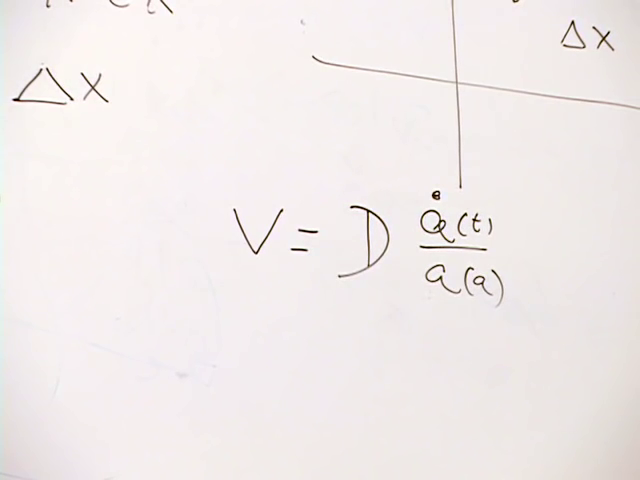
\includegraphics[width=0.68\textwidth]{lecture_07_figure_12.png}
\caption{黒板に書かれた等時後退法則：\(V=D\,\dot a/a\)。}
\lectureframe{01:29:10.000}
\end{figure}

``ハッブル定数''という名称は誤解を招きうる。一般に\(H(t)\)は時間とともに変化する。空間的に一定なのは、同じ時間スライス上のあらゆる共動点の対に対する比\(V/D\)である。

\begin{classroomqa}
\audiencequestion{遠方の銀河について、この関係に現れる時刻は誰の時刻か。我々はそれらをより早い時代に観測する。\lecturetimestamp{01:31:10}}
\lecturerresponse{式~\eqref{eq:l07-hubble-law}は等時的な主張である。観測は過去向きの光線に沿って進み、遠方の銀河をより早い時刻にサンプルする。したがって、測定された赤方偏移と距離の関係には、\(H\)の一瞬の値ではなく、光円錐の全履歴が必要である。}
\end{classroomqa}

\begin{figure}[htbp]
\centering
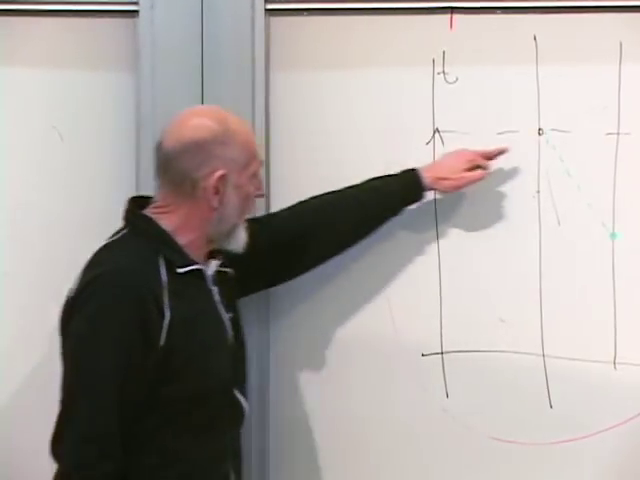
\includegraphics[width=0.66\textwidth]{lecture_07_figure_13.png}
\caption{等時的分離と、観測者が過去の光線に沿って見るものとを区別するために用いられる時空のスケッチ。}
\lectureframe{01:33:20.000}
\end{figure}

\section{ハッブルスケールとド・ジッター膨張}

単位\(c=1\)では、式~\eqref{eq:l07-hubble-law}は距離
\begin{equation}
D_H=\frac{1}{H}.
\label{eq:l07-hubble-radius}
\end{equation}
において後退速度を1に定める。より遠方の共動点は、特殊相対性理論に違反することなく\(V>1\)、あるいは\(V\gg1\)さえ持ちうる。それらは局所的な観測者を光より速く通過するのではない。それらの固有分離は、間にある幾何が膨張するために増大する。\editorialnote{一般の時間依存の宇宙論では、\(1/H\)はハッブル半径であり、自動的に事象の地平面になるわけではない。次に議論するド・ジッターの場合には、それが一定の地平面スケールとなる。}

多くの古い減速する宇宙論的模型では、\(H(t)\)は減少し\(1/H(t)\)は増大するので、かつて超光速で後退していた領域が後に因果的接触に入りうる。講義で議論される晩期の描像は、代わりに正の定数\(H\)に近づく。すると\(1/H\)は固定されたままであり、膨張方程式は
\begin{equation}
\frac{\dot a}{a}=H,
\qquad
\dot a=Ha.
\label{eq:l07-constant-h}
\end{equation}
となる。

\begin{classroomqa}
\audiencequestion{一定のハッブルパラメータの単位は何か。\lecturetimestamp{01:38:24}}
\lecturerresponse{時間の逆数である。等価に、\(c=1\)とすれば、長さの逆数である。量\(H^{-1}\)は膨張時間と距離スケールの両方を与える。講義では約150億年という桁の例を用いている。}
\end{classroomqa}

式~\eqref{eq:l07-constant-h}の解は
\begin{equation}
a(t)=a_0e^{Ht}.
\label{eq:l07-desitter-scale-factor}
\end{equation}
である。

\begin{classroomqa}
\audiencequestion{それ自身に比例する変化率を持つ関数は何か。\lecturetimestamp{01:39:04}}
\lecturerresponse{指数関数である。したがってスケール因子は\(a_0e^{Ht}\)であり、一方、計量における空間係数\(a(t)^2\)は\(e^{2Ht}\)として増大する。}
\end{classroomqa}

\begin{figure}[htbp]
\centering
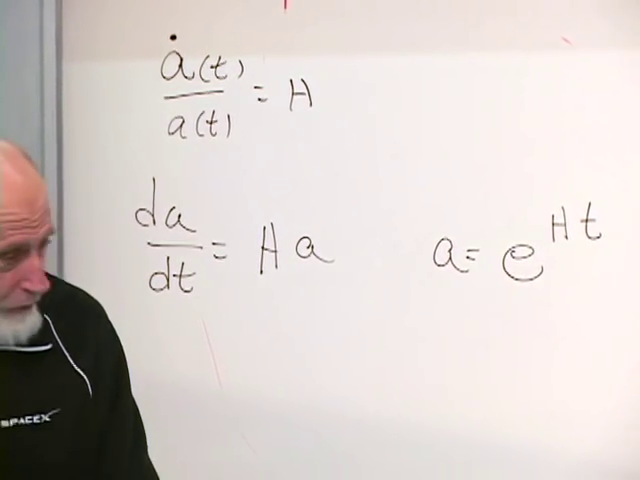
\includegraphics[width=0.70\textwidth]{lecture_07_figure_14.png}
\caption{黒板に書かれた一定の\(H\)に対する方程式とその指数関数解。}
\lectureframe{01:39:30.000}
\end{figure}

この指数的膨張を持つ時空はド・ジッター空間である。その一定のハッブルスケールは有限の固有距離に事象の地平面を生じる。この幾何はある意味でブラックホールの描像の補集合である。観測者は宇宙論的地平面の内側にとどまり、十分遠方の物体は後退して、観測者を捕まえる信号を決して送ることができない。ブラックホールの地平面は内部を外部の観測者から隠す。ド・ジッターの地平面は、観測者の到達可能なパッチの外部を隠す。普通の蒸発するブラックホールとは異なり、理想的なド・ジッター幾何はここでは持続するものとして扱われる。この比較はここで始まったばかりである。次の講義では、地平面、その熱力学、そしてそれが宇宙論にもたらす難題を展開する。

\chapter{真空のエネルギーとド・ジッター地平線}

\lectureoverview{真空のエネルギーは通常の物質とは異なる。それは特別な慣性系を選び出すこともなく、宇宙の膨張に伴って薄まることもない。重力を含めると、一見無害に見えるこのエネルギーの零点が時空の幾何学を変える。物質優勢の法則 \(a(t)\propto t^{2/3}\) を導出し、それを真空優勢の法則 \(a(t)\propto e^{Ht}\) と対比し、次にド・ジッター時空を共形座標で書き直す。得られる因果図は、固有距離が固定された観測者依存の事象の地平線を明らかにする。}

\section{真空における量子揺らぎ}

本講義全体の動機となる問いから始めよう。量子場の理論は空っぽの空間にエネルギーを割り当てる。これは、実在の電子--陽電子対が絶えず無から現れているということを意味するのだろうか。

\begin{classroomqa}
\audiencequestion{電子--陽電子の生成と消滅は実際に真空で起こっているのか、それとも単なる帳簿上の操作にすぎないのか。\lecturetimestamp{00:00:06}}
\lecturerresponse{仮想対は真空のエネルギーに寄与するが、それらは空っぽの空間から現れるのを観察できる通常の粒子ではない。それらは量子基底状態の揺らぎであり、仮想過程にふさわしい制限の範囲内でのみ持続する。}
\end{classroomqa}

調和振動子が最も明快な模型を与える。古典的には、それはポテンシャルの最小点で静止したままでいられる。量子力学的には、最小点における正確な位置と正確にゼロの運動量は両立しない。基底状態は両者の間で妥協し、零点エネルギー
\begin{equation}
E_0=\frac{1}{2}\hbar\omega.
\label{eq:l08-zero-point}
\end{equation}
を保つ。これが振動子の持ちうる最小のエネルギーである。これは励起状態ではなく、観測可能な粒子の流れを表すものでもない。

自由場は規準モードに分解され、各モードは振動子のように振る舞う。空洞内の電磁場はよく知られた例である。すべてのモードが式~\eqref{eq:l08-zero-point}の形の項に寄与し、電子、クォーク、その他の量子場もそれぞれ独自の基底状態の揺らぎに寄与する。これらの寄与を足し合わせたものが、我々が真空のエネルギーと呼ぶものである。素朴な微視的見積もりと観測された宇宙論的スケールとの間の悪名高い不一致は実在するが、それは本講義の主題ではない。

\begin{classroomqa}
\audiencequestion{およそ \(120\) 桁の不一致について再び議論されるのだろうか。\lecturetimestamp{00:02:59}}
\lecturerresponse{ここでは扱わない。当面の目標は宇宙論的地平線を理解することである。すなわち、宇宙論の方程式がどのように加速膨張を生み出すのか、そしてなぜ加速膨張が事象の地平線を生み出すのかである。}
\end{classroomqa}

\begin{classroomqa}
\audiencequestion{前回の講義の紫外--赤外の関係は今夜の議論の一部なのだろうか。\lecturetimestamp{00:03:59}}
\lecturerresponse{後で再び取り上げるかもしれないが、予定された論証の一部ではない。当面の道筋は真空のエネルギーから宇宙論へ、そして地平線へと進む。}
\end{classroomqa}

\section{なぜ真空のエネルギーはローレンツ不変なのか}

次の問いは初歩的に見えるが、真空のエネルギーの定義的な性質を露わにする。もし空っぽの空間が正のエネルギー密度を持つなら、なぜそれは光学媒質のように振る舞い、光の速さを変えないのか。

\begin{classroomqa}
\audiencequestion{正の真空のエネルギー密度は屈折効果を持ち、光をわずかに遅く進ませるべきではないのか。\lecturetimestamp{00:04:35}}
\lecturerresponse{通常の物質はそれが可能である。なぜならそれは特別な静止系を定義するからである。真空のエネルギーは異なる。それはそのような系を選び出さず、すべての慣性観測者が同じ真空のエネルギー密度を得る。したがって光の局所的な測定は不変の速さ \(c\) を保つ。}
\end{classroomqa}

法則の対称性と特定の状態の対称性を区別しなければならない。物理学の方程式は並進不変でありえても、スタンフォードはバークリーではなく、地球は星間空間ではない。\emph{物理的配置全体}を並進させても法則は変わらない。物質の実際の配置は、あらゆる場所で同じに見える必要はない。同様に、回転不変な方程式はこの教室を回転対称にするものではない。

同じ区別がローレンツ変換にも当てはまる。気体には静止系がある。それを通り抜けて運動する観測者は運動する分子と異なるエネルギー密度を見るので、気体の状態は、それを支配する方程式がローレンツ不変であっても、ローレンツ不変ではない。通常の物質、放射浴、実験装置はすべて、特別な運動や方向を選び出すことによって対称性を破る。

真空のエネルギーは、そうしない例外的な形態の物質である。真空エネルギーの密度を報告する検出器を想像しよう。静止しているとき、それはある値\(\rho_{\rm vac}\)を与える。検出器を加速して測定を繰り返す。結果は変わらない。相対論的表記では、この性質は計量に比例する応力テンソルによって表される。
\begin{equation}
T_{\mu\nu}^{\rm vac}=-\rho_{\rm vac}g_{\mu\nu},
\qquad
p_{\rm vac}=-\rho_{\rm vac}.
\label{eq:l08-vacuum-stress}
\end{equation}
\editorialnote{圧力の関係は板書では導出されない。それは講義の二つの定義的性質、すなわちローレンツ不変性と膨張中の一定密度の背後にある共変的な言明である。}

局所的な但し書きが重要である。観測者のそばを通過する光線は、近くの時計と物差しで測ると\(c\)で進む。膨張する幾何学において、遠方の光線の私たちに対する速さを問うには、座標の選択と、遠く離れた事象を比較するための規定が必要である。その座標速度は\(c\)に等しい必要はない。すべての局所的な観測者が\(c\)を測定するとしても、である。

\begin{classroomqa}
\audiencequestion{この議論において、真空エネルギーと宇宙定数は同義ですか。\lecturetimestamp{00:11:57}}
\lecturerresponse{はい。それらはアインシュタイン方程式における同じ項の二つの配置である。幾何学の側では宇宙定数として記述され、源の側ではローレンツ不変な真空の応力エネルギーとして記述されうる。}
\end{classroomqa}

\section{何が薄まり、何が薄まらないか}

質量\(m\)の非相対論的粒子で大きな領域を満たす。銀河や銀河団を平均するのに十分大きなスケールでは、分布は一様であると仮定する。共動体積が\(N\)個の粒子を含むなら、その物質密度は
\begin{equation}
\rho_m=\frac{Nm}{V}.
\end{equation}
である。すべての線形の長さが二倍になると、体積は\(2^3=8\)倍に増えるが、\(N\)と\(m\)は変わらない。したがって密度は以前の値の八分の一に下がる。通常の物質が薄まるのは、同じ粒子がより大きな物理的体積を占めるからである。

輻射も薄まり、しかもより速く薄まる。その数密度は体積とともに下がり、一方で各光子の波長は引き伸ばされ、そのエネルギーは赤方偏移する。後に結果\(\rho_r\propto a^{-4}\)を記録するが、今夜は輻射優勢の宇宙論を解かない。

真空エネルギーは例外である。
\begin{equation}
\rho_{\rm vac}(t)=\text{constant}.
\label{eq:l08-rho-vac-constant}
\end{equation}
それは集団化せず、方向を選ばず、慣性系を選ばず、空間が膨張しても密度が小さくならない。共動する箱が大きくなれば、その中に含まれる真空エネルギーはその体積に比例して増える。

\editorialnote{一定密度とは、膨張する共動する箱の内部の全真空エネルギーが一定であることを意味しない。共変的な応力エネルギーの保存
\(\dot\rho+3H(\rho+p)=0\)は、真空エネルギーが負の圧力\(p_{\rm vac}=-\rho_{\rm vac}\)をもつために満たされる。仕事の項が、箱の全真空エネルギーの変化をちょうど供給する。}

\section{重力はエネルギーの零点を見る}

非重力の実験室物理学では、すべてのエネルギーを同じ定数だけずらしても通常は何も変わらない。スペクトルは差に依存する。励起した原子と励起していない原子の間のエネルギー、あるいは粒子がある状態とない状態の間のエネルギーである。空の空間は、その絶対エネルギーを測る基準を何も提供しないように見える。

重力は問いを変える。質量はエネルギーであり、エネルギーは重力の源であり、したがって真空エネルギーは重力を及ぼす。原子遷移では見えなかった定数が時空を曲げうる。

アインシュタイン方程式は幾何学と源を分ける。
\begin{equation}
G_{\mu\nu}=8\pi G_N T_{\mu\nu},
\label{eq:l08-einstein}
\end{equation}
ここで単位は\(c=1\)である。アインシュタインテンソル\(G_{\mu\nu}\)は計量\(g_{\mu\nu}(x)\)とその導関数から作られる。応力テンソル\(T_{\mu\nu}\)は、物質および非重力場からのエネルギー密度、運動量密度、圧力、応力を含む。真空エネルギーは通常の物質とまったく同様にこの源の側に属する。\editorialnote{口頭の導入は\(8\pi/3\)をテンソル方程式と簡単に結びつける。因子\(1/3\)は以下の空間的に平坦なフリードマン方程式に属し、式~\eqref{eq:l08-einstein}には属さない。}

\begin{figure}[htbp]
\centering
\includegraphics[width=0.62\textwidth]{lecture_08_figure_02.png}
\caption{時空計量\(g_{\mu\nu}(x)\)から作られるアインシュタイン方程式の幾何学の側。}
\lectureframe{00:21:58.820}
\end{figure}

\section{幾何学はスケール因子に還元される}

ここで、平坦な空間的断面をもつ最も単純な一様膨張幾何学を選ぶ。
\begin{equation}
ds^2=-dt^2+a(t)^2\,d\mathbf{x}^2,
\qquad
d\mathbf{x}^2=dx^2+dy^2+dz^2.
\label{eq:l08-frw-metric}
\end{equation}
座標の印\(\mathbf{x}\)は無限のゴムシートに描かれている。それらは動く必要はないが、それらの物理的間隔は動く。\(\Delta\mathbf{x}\)だけ離れた二つの共動点は、\(t\)を固定したとき固有距離
\begin{equation}
D(t)=a(t)\lvert\Delta\mathbf{x}\rvert.
\label{eq:l08-proper-distance}
\end{equation}
をもつ。したがって、この高度に対称な幾何学の時間依存性はすべて一つの関数、スケール因子\(a(t)\)に蓄えられる。\(a\)が一定なら、空間的再スケーリングの後で平坦なミンコフスキー時空を与える。\(a\)が時間に依存すれば、各空間的断面を平坦に保ちながら、時空全体を曲がったものにしうる。

\begin{classroomqa}
\audiencequestion{座標マーク\(x=7\)と\(x=13\)について、それらの座標間隔は\(4\)か。\lecturetimestamp{00:27:40}}
\lecturerresponse{いいえ。それは\(13-7=6\)であり、したがってそれらの物理的間隔は\(6a(t)\)である。この補正は有用である。\(x\)は共動位置を表し、一方\(a(t)\)を掛けると物理的距離が得られる。}
\end{classroomqa}

この計量と空間的に一様なエネルギー密度に対して、アインシュタイン方程式の一つの成分が空間的に平坦なフリードマン方程式となる。
\begin{equation}
\left(\frac{\dot a}{a}\right)^2
=\frac{8\pi G_N}{3}\rho(t).
\label{eq:l08-friedmann}
\end{equation}
比
\begin{equation}
H(t)\equiv\frac{\dot a(t)}{a(t)}
\label{eq:l08-hubble-definition}
\end{equation}
はハッブルパラメータである。これはこの段階では定義であり、時間とともに変化しうる。

\begin{figure}[htbp]
\centering
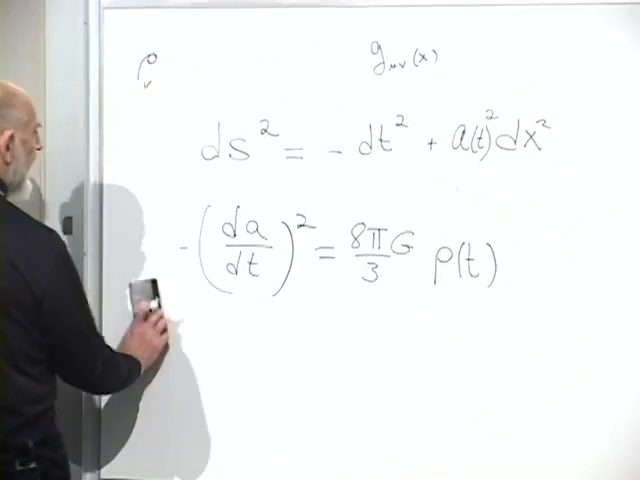
\includegraphics[width=0.90\textwidth]{lecture_08_figure_03.png}
\caption{黒板で欠けていた因子\(1/a^2\)が復元された後の、平坦膨張計量とフリードマン方程式。}
\lectureframe{00:30:30.000}
\end{figure}

\paragraph{エネルギー収支の描像。}
このエネルギー収支の描像に対して、式~\eqref{eq:l08-friedmann}は模式的に
\begin{equation}
-\frac{3}{8\pi G_N}H^2+\rho=0.
\label{eq:l08-energy-heuristic}
\end{equation}
と書ける。物質エネルギーは正であり、一方、膨張するスケール因子によって表される重力自由度は負の運動項を持つ。この縮約された問題では、負の重力エネルギーと正の物質エネルギーの和がゼロに等しいことが有用な記憶法である。

\editorialnote{式~\eqref{eq:l08-energy-heuristic}は高度に対称なミニスーパースペース模型におけるハミルトニアン拘束条件であり、任意の宇宙がゼロに等しい大域的に保存された全エネルギーを持つという座標に依存しない定理ではない。講義ではこれをフリードマン拘束条件のヒューリスティックな解釈として用いている。}

\section{物質優勢膨張}

座標の辺の長さが\(\Delta x=1\)である共動的な数学的箱に戻る。その物理的な辺の長さは\(a(t)\)であり、したがってその物理的体積は\(a(t)^3\)である。もし質量\(m\)の非相対論的粒子を\(N\)個含むならば、
\begin{equation}
\rho_m(t)=\frac{Nm}{a(t)^3}
=\frac{\rho_0}{a(t)^3}.
\label{eq:l08-matter-density}
\end{equation}
粒子自体は膨張しない。それらの平均間隔が膨張するのである。

\begin{figure}[htbp]
\centering
\includegraphics[width=0.84\textwidth]{lecture_08_figure_04.png}
\caption{共動箱の議論を組み立てた際の計量とフリードマン方程式。}
\lectureframe{00:36:07.940}
\end{figure}

式~\eqref{eq:l08-friedmann}に代入すると
\begin{equation}
\left(\frac{\dot a}{a}\right)^2
=\frac{8\pi G_N\rho_0}{3a^3}.
\end{equation}
\(K=8\pi G_N\rho_0/3\)と書き、膨張する枝を選ぶ。
\begin{align}
\dot a^2&=\frac{K}{a},\\
\dot a&=\sqrt{K}\,a^{-1/2},\\
a^{1/2}\,da&=\sqrt{K}\,dt.
\label{eq:l08-matter-separated}
\end{align}

\begin{classroomqa}
\audiencequestion{分離された方程式はどのように解くべきか。\lecturetimestamp{00:38:15}}
\lecturerresponse{両辺を積分する。\(a^{1/2}\,da\)の積分は\(\frac{2}{3}a^{3/2}\)であり、\(\frac{3}{2}a^{3/2}\)ではない。\(\frac{3}{2}\)が新しい冪であり、一方\(\frac{2}{3}\)は係数である。}
\end{classroomqa}

したがって、
\begin{equation}
\frac{2}{3}a^{3/2}
=\sqrt{K}\,(t-t_B),
\end{equation}
ここで\(t_B\)は選ばれた時間の原点を固定する積分定数である。規格化と時間のずれを除けば、
\begin{equation}
a(t)\propto (t-t_B)^{2/3}.
\label{eq:l08-matter-solution}
\end{equation}

\begin{figure}[htbp]
\centering
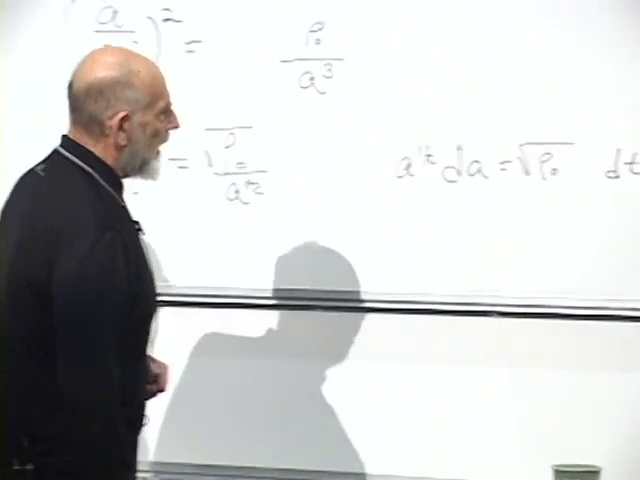
\includegraphics[width=0.86\textwidth]{lecture_08_figure_05.png}
\caption{物質密度の代入と変数分離により\(a^{1/2}da\propto dt\)が導かれる。}
\lectureframe{00:38:30.000}
\end{figure}

曲線\(t^{2/3}\)は直線よりもゆっくりと増加する。その傾きは減少するので、物質優勢宇宙は減速する。講義で用いられたニュートン的な言葉では、粒子は最初に離れ始め、それらの相互の重力引力が離れる割合を絶えず減少させる。

\begin{figure}[htbp]
\centering
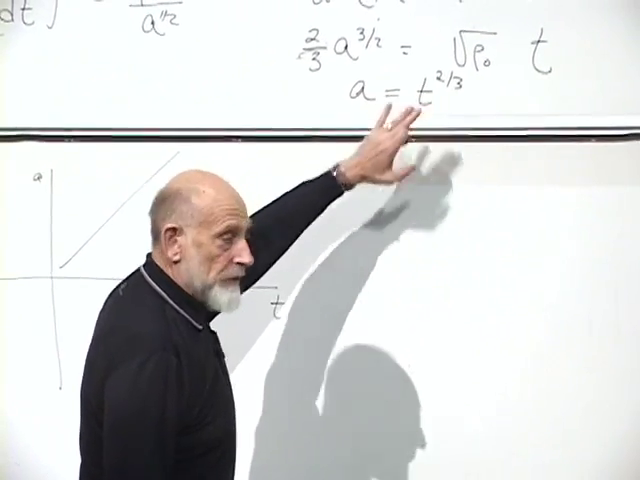
\includegraphics[width=0.86\textwidth]{lecture_08_figure_06.png}
\caption{線形膨張と下に凸な物質法則\(a(t)\propto t^{2/3}\)の黒板上での比較。}
\lectureframe{00:40:00.000}
\end{figure}

参考までに、放射浴は
\begin{equation}
\rho_r\propto a^{-4},
\end{equation}
であり、\(a^{-3}\)ではない。体積の希釈が三つの冪を寄与し、宇宙論的赤方偏移がもう一つ寄与する。対応するスケール因子も解くことができるが、講義ではその演習を意図的に脇に置いている。

\section{真空優勢膨張}

ここでフリードマン方程式の右辺に真空エネルギーのみを置く。\(\rho_{\rm vac}\)は定数であるから、
\begin{equation}
\left(\frac{\dot a}{a}\right)^2
=\frac{8\pi G_N}{3}\rho_{\rm vac}
\equiv H^2.
\label{eq:l08-de-sitter-friedmann}
\end{equation}
\(H\)の二つの用法を区別しておく必要がある。式~\eqref{eq:l08-hubble-definition}は時間に依存しうる量\(\dot a/a\)を定義する。式~\eqref{eq:l08-de-sitter-friedmann}は、純粋な真空エネルギー宇宙においてその値が定数
\begin{equation}
H=\sqrt{\frac{8\pi G_N\rho_{\rm vac}}{3}}.
\end{equation}
であることを述べている。膨張する枝を取ると
\begin{equation}
\dot a=Ha,
\end{equation}
となり、したがって
\begin{equation}
a(t)=C e^{Ht}.
\label{eq:l08-exponential-solution}
\end{equation}
となる。積分定数\(C\)は共動座標の任意の規格化を固定する。\(a\)の現在の値に比例する成長は指数関数的成長である。

\begin{figure}[htbp]
\centering
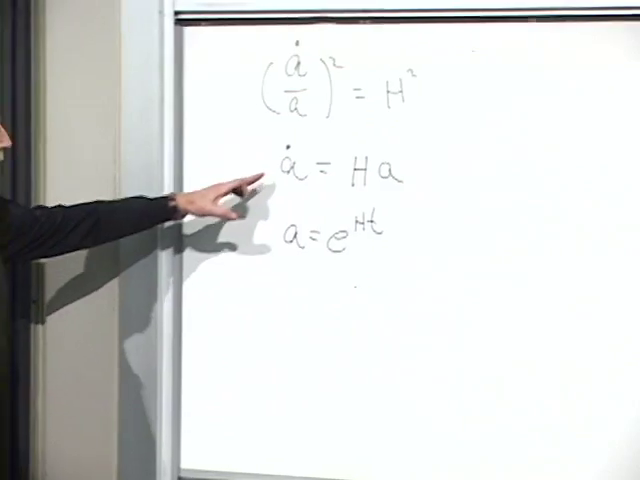
\includegraphics[width=0.88\textwidth]{lecture_08_figure_07.png}
\caption{真空優勢方程式\((\dot a/a)^2=H^2\)、その一階の形\(\dot a=Ha\)、および指数関数解。}
\lectureframe{00:47:45.000}
\end{figure}

共動物体に対するハッブル則は
\begin{equation}
v_{\rm rec}=HD.
\label{eq:l08-hubble-law}
\end{equation}
である。この純粋なド・ジッターの場合、後退速度が\(c\)に等しくなる固有距離は一定である。
\begin{equation}
D_H=\frac{c}{H},
\label{eq:l08-hubble-radius}
\end{equation}
または、黒板で用いられた\(c=1\)の単位では\(D_H=H^{-1}\)である。この固定されたスケールは、ド・ジッター事象の地平面半径として幾何学的に再び現れる。\editorialnote{ハッブル半径は、任意の時間依存宇宙論において自動的に事象の地平面となるわけではない。この同定がここで成り立つのは、厳密なド・ジッター空間において\(H\)が定数であるからである。}

この講義では、真空エネルギー検出器のための思考実験を提示する。他の源から遠く離れた、ごく軽い二つの試験体を、共動流に対して初め静止した状態に置き、それらの相互引力を無視できるようにする。それらの間隔は指数関数的膨張に従う。この効果は地上の装置にはあまりにも小さすぎるが、宇宙的距離と過去を見る時間によって、同じ物理が観測可能になる。

\section{物質支配から真空支配へ}

この講義で考察される実際の宇宙論的モデルには両方の項が含まれる：
\begin{equation}
H(t)^2
=\frac{8\pi G_N}{3}
\left(\frac{\rho_0}{a(t)^3}+\rho_{\rm vac}\right).
\label{eq:l08-mixed-friedmann}
\end{equation}
小さい\(a\)では、\(a^{-3}\)が大きいため物質項が支配し、解は\(t^{2/3}\)に似る。宇宙が成長するにつれて、物質は希薄化する一方で真空エネルギーは一定に留まる。やがて定数項が勝ち、スケール因子は\(e^{Ht}\)に向かって上向きに曲がる。

\begin{figure}[htbp]
\centering
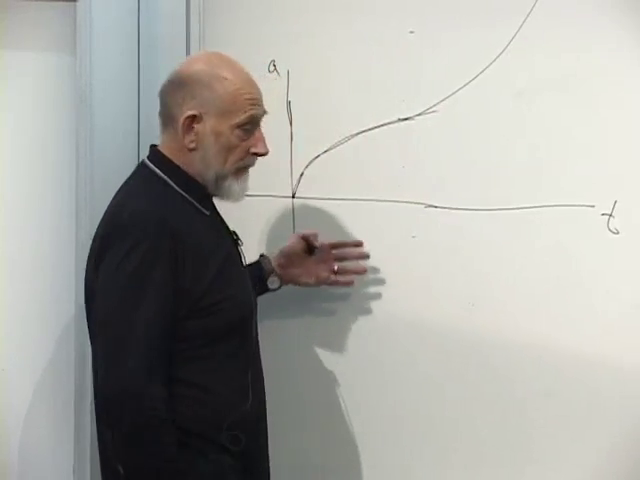
\includegraphics[width=0.87\textwidth]{lecture_08_figure_08.png}
\caption{この講義で描かれた定性的な転移：初期の物質支配による減速に続く、後期の真空支配による指数関数的成長。}
\lectureframe{00:53:30.000}
\end{figure}

\begin{classroomqa}
\audiencequestion{指数関数的解には積分定数が含まれる。それが極端に小さくないと、どうして分かるのか。\lecturetimestamp{00:52:41}}
\lecturerresponse{それを測定する。宇宙のより遠くを見ることは、より遠い過去を見ることを意味するので、異なる距離での観測は、膨張曲線の今日の値だけでなく、その初期部分を再構成する。}
\end{classroomqa}

この講義は、当時利用可能であった後期の観測が約5パーセントの水準で指数関数的な枝と整合していたと報告し、その証拠を説得力があると述べているが、電子の性質のような精密測定ほど厳密ではないとしている。これは現在の精密な主張としてではなく、講義当時の歴史的評価として読むべきである。

\begin{classroomqa}
\audiencequestion{上向きに曲がる膨張曲線は、最終的に我々が観測をビッグバンや宇宙マイクロ波背景放射まで遡ることを妨げるのか。\lecturetimestamp{00:55:05}}
\lecturerresponse{それはグラフの外挿に関する問題としては追及されない。関連する不変的な問題は事象の地平面の存在であり、それが今から扱う因果的な問題である。}
\end{classroomqa}

\section{束縛系と遠い未来}

指数関数的膨張が続くなら、希薄化するすべての成分は\(\rho_{\rm vac}\)に比べて無視できるようになる。これは、原子、太陽系、銀河それ自体が引き伸ばされるという意味ではない。束縛されたままでいるのに十分強く結びついた系はハッブル流に従わない。

\begin{classroomqa}
\audiencequestion{今日膨張していない銀河は、真空エネルギーが支配するようになると最終的に膨張するのか。\lecturetimestamp{00:57:44}}
\lecturerresponse{束縛系は束縛されたままである。天の川銀河とアンドロメダ銀河は、共に留まる近傍の構造に属するが、膨張とともにすでに運動している十分遠方の銀河は外へ進み続け、最終的に我々の地平面の向こうへと通過する。}
\end{classroomqa}

\emph{引き付けられている}ことと\emph{束縛されている}ことの区別は本質的である。脱出速度を超えて打ち上げられたロケットは地球の引力の下にあり続けるが、それでも戻ってこない。同様に、二つの銀河間の最大の局所的な力が通常の重力引力であっても、それらの相対軌道が束縛されているとは限らない。

\begin{classroomqa}
\audiencequestion{我々の銀河は重力によって集団と結びついている。加速膨張は最終的にその引力を打ち負かすのか。\lecturetimestamp{00:59:17}}
\lecturerresponse{局所構造の真に束縛された部分だけが共に留まる。銀河団という記述的なラベルだけでは十分ではない；束縛されているとは、相対運動が脱出以下にあることを意味する。より遠方の銀河は引き付けられていても、脱出速度を超えて後退することがある。}
\end{classroomqa}

直観のために、この講義は相対的な動径加速度を、引力の逆二乗項と間隔に線形な真空項の和として模式的に表す：
\begin{equation}
\ddot r\sim-\frac{G_NM}{r^2}+H^2r.
\label{eq:l08-newtonian-vacuum}
\end{equation}
理想化されたド・ジッター極限では係数は時間に依存しない。第二項が増大するのは\(r\)が増大するからだけであり、\(G_N\)が徐々に弱まることから生じるのではない。

\editorialnote{式~\eqref{eq:l08-newtonian-vacuum}はニュートン的な相対加速度のヒューリスティックであり、一般相対性理論に根本的な追加の力の法則ではない。厳密なド・ジッター空間では、隣接する自由落下世界線の相対加速度は\(H^2r\)に比例する。}

\begin{figure}[htbp]
\centering
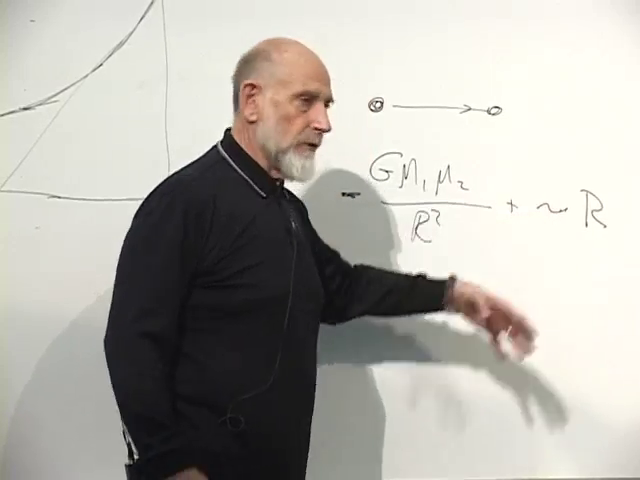
\includegraphics[width=0.88\textwidth]{lecture_08_figure_09.png}
\caption{逆二乗引力と、間隔に線形に増大する実効的な真空の斥力との黒板での比較。}
\lectureframe{01:04:10.000}
\end{figure}

\begin{classroomqa}
\audiencequestion{外向きの効果自体は時間とともに増大するのか。\lecturetimestamp{01:01:18}}
\lecturerresponse{固定した間隔では増大しない。その係数は一定である。自由に後退する物体は互いに遠ざかり、\(r\) に比例する項は、それらの距離が大きいために大きくなる。}
\end{classroomqa}

\begin{classroomqa}
\audiencequestion{正味の効果はニュートン定数の漸進的な減少として記述できるのか。\lecturetimestamp{01:02:30}}
\lecturerresponse{いいえ。\(G_N\) は一定のままである。指定された間隔では両方の係数は変わらず、\(1/r^2\) の引力と \(r\) に比例する項の相対的な重要性だけが距離とともに変化する。}
\end{classroomqa}

\begin{classroomqa}
\audiencequestion{真空エネルギーが重要になる前の初期宇宙において、同じ銀河は重力で束縛されていたのか。\lecturetimestamp{01:05:03}}
\lecturerresponse{通常の引力が支配的であること自体は、束縛を意味しない。多くの銀河はすでに脱出速度程度かそれ以上で互いに離れつつあった。真空エネルギーは後に、大規模な膨張が再収縮に向かって減速するか、それとも加速して遠ざかるかを決めるが、最大の力と束縛軌道は別の主張である。}
\end{classroomqa}

したがって、遠い未来の観測者は、合体した局所構造の中に住む一方で、束縛されていないすべての銀河は観測不可能になっているかもしれない。歴史的記録がなければ、その観測者はほとんど空の宇宙を推論しても妥当であろう。この因果的な孤独こそが、局所的な物体の破壊ではなく、地平線への物理的な導入である。

\section{事象の地平線が意味するもの}

休憩の後、
\begin{equation}
a(t)=e^{Ht}
\end{equation}
と置き、計量を
\begin{equation}
ds^2=-dt^2+e^{2Ht}d\mathbf{x}^2.
\label{eq:l08-de-sitter-metric}
\end{equation}
と書く。

\begin{classroomqa}
\audiencequestion{この計量が記述する時空の名前は何か。\lecturetimestamp{01:08:13}}
\lecturerresponse{それはド・ジッター時空であり、通常はド・ジッター空間と略される。その地平線が重要であるのは、真空が支配的な宇宙が後期にこの幾何学に近づくからである。}
\end{classroomqa}

その因果構造を描く前に、ペンローズ図の役割を思い出そう。無限の区間は、ヌル光線が \(45^\circ\) にとどまるまま、有限の図に圧縮される。平坦な時空では、質量をもつ物体は未来の時間的無限遠で終わり、ヌル光線はヌル無限遠で終わり、任意に長く待つことを許された慣性観測者には、時空の永続的な領域を排除する事象の地平線は存在しない。

\begin{figure}[htbp]
\centering
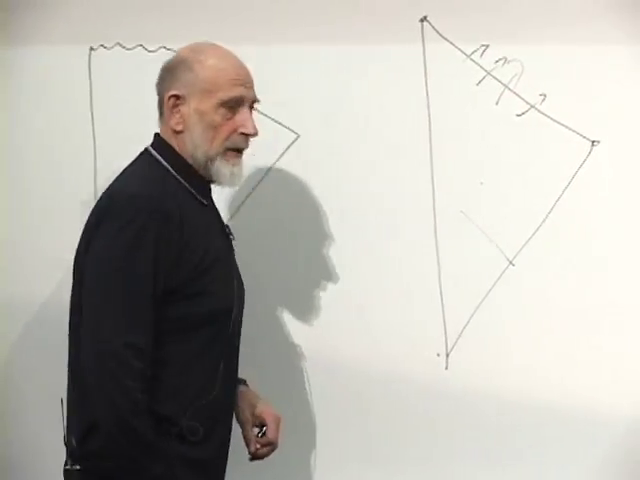
\includegraphics[width=0.80\textwidth]{lecture_08_figure_10.png}
\caption{地平線を導入する前に、時間的およびヌルの行き先を区別するために用いられる平坦時空のペンローズ図。}
\lectureframe{01:10:35.000}
\end{figure}

ブラックホールの図は対照を与える。外部の観測者は、観測者の未来の世界線の因果的過去にある事象からのみ信号を受け取ることができる。観測時間が無限大に近づいても、内部領域は排除されたままである。その観測者と通信できる事象と決してできない事象との境界が事象の地平線である。

\begin{definition}
観測者の未来の事象の地平線とは、未来向きの因果的信号がその観測者の世界線にいつか到達しうる事象の集合の境界である。
\label{def:l08-event-horizon}
\end{definition}

\begin{figure}[htbp]
\centering
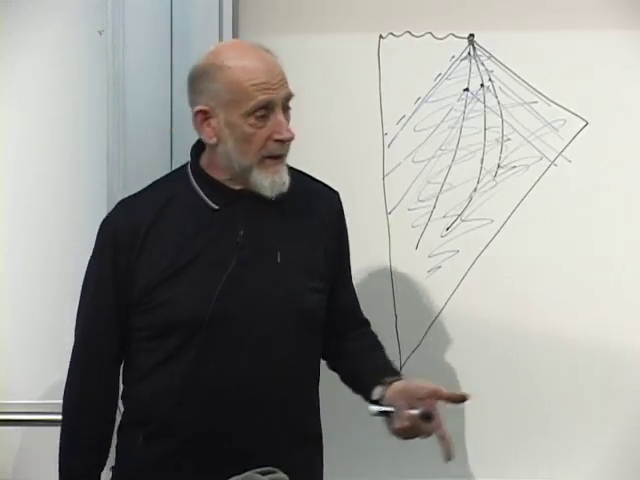
\includegraphics[width=0.80\textwidth]{lecture_08_figure_11.png}
\caption{ブラックホールとの比較：任意に遅い外部観測からの過去光円錐は、事象の地平線の向こう側の領域を決して含まない。}
\lectureframe{01:13:50.000}
\end{figure}

したがって事象の地平線は大域的な因果的境界であり、単に物体が今日たまたま暗く見える距離ではない。それを特定するには、任意に長く待った後でもどの信号が到達しうるかを知らなければならない。

\section{無限の未来を圧縮する}

式~\eqref{eq:l08-de-sitter-metric} の空間座標はすでに無限の平坦なスライスにわたっている。それらはそのままにし、時間だけを圧縮する。共形時間 \(T\) を
\begin{equation}
dt^2=e^{2Ht}dT^2.
\label{eq:l08-conformal-definition}
\end{equation}
を要求することによって導入する。未来向きの平方根をとり、整理すると
\begin{equation}
dT=e^{-Ht}dt.
\end{equation}
が得られる。

\begin{classroomqa}
\audiencequestion{符号を含め、その積分は何か。\lecturetimestamp{01:17:25}}
\lecturerresponse{それは \(-H^{-1}e^{-Ht}\) である。付加定数は \(T\) の原点をずらすだけなので、無限の未来を \(T=0\) に置くように選ぶ。}
\end{classroomqa}

したがって
\begin{equation}
T=-\frac{1}{H}e^{-Ht},
\qquad -\infty<T<0.
\label{eq:l08-conformal-time}
\end{equation}
\(t\to-\infty\) のとき、\(T\to-\infty\)。固有時間 \(t\to+\infty\) のとき、\(T\to0^{-}\)。無限の未来は有限の水平線 \(T=0\) 上に置かれた。どの観測者も有限の固有時間ではそこに到達しない。

\begin{figure}[htbp]
\centering
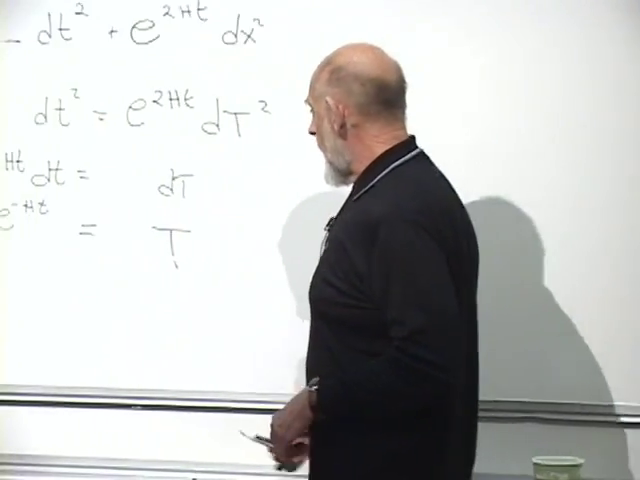
\includegraphics[width=0.86\textwidth]{lecture_08_figure_12.png}
\caption{共形時間の積分と、無限の未来 \(t\to+\infty\) の \(T=0^{-}\) への写像。}
\lectureframe{01:19:10.000}
\end{figure}

式~\eqref{eq:l08-conformal-time} から、
\begin{equation}
HT=-e^{-Ht},
\qquad
e^{2Ht}=\frac{1}{H^2T^2}.
\label{eq:l08-conformal-factor}
\end{equation}
式~\eqref{eq:l08-de-sitter-metric} で \(dt=e^{Ht}dT\) を用いると、
\begin{equation}
ds^2=\frac{1}{H^2T^2}
\left(-dT^2+d\mathbf{x}^2\right).
\label{eq:l08-conformal-metric}
\end{equation}
が得られる。括弧内の表式はミンコフスキー計量である。ド・ジッター幾何学はすべて、\(T\to0^{-}\) のとき発散する共通の共形因子の中に入っている。

\begin{figure}[htbp]
\centering
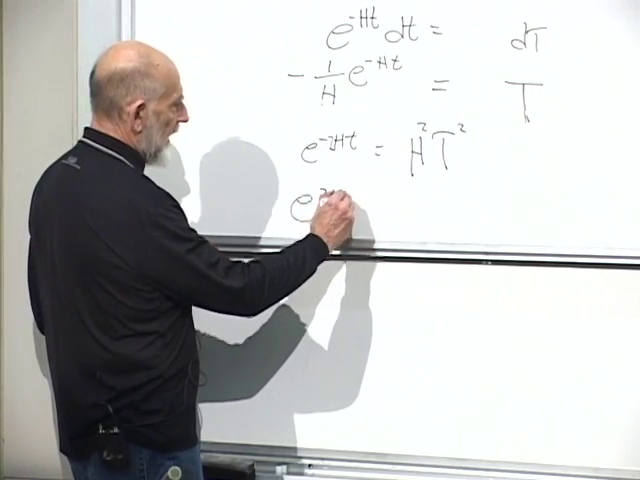
\includegraphics[width=0.87\textwidth]{lecture_08_figure_13.png}
\caption{\(e^{2Ht}\) を \(1/(H^2T^2)\) に関係づけ、計量の共形形を準備する代数。}
\lectureframe{01:22:50.000}
\end{figure}

\begin{classroomqa}
\audiencequestion{この計量において、光線の経路はどのような条件で決まるのですか。\lecturetimestamp{01:23:49}}
\lecturerresponse{光線はヌル経路 \(ds^2=0\) に従う。したがって共通の共形因子は相殺され、選んだ空間方向に沿って \(dT=\pm dx\) が残る。}
\end{classroomqa}

光線は \((T,x)\) 図において \(45^\circ\) の直線である：
\begin{equation}
\frac{dx}{dT}=\pm1.
\label{eq:l08-null-lines}
\end{equation}
座標による描像は \(T=0\) の近くでひどく圧縮されているが、必要なこと、すなわちどの事象が通信できるかを正確に保っている。

\begin{figure}[htbp]
\centering
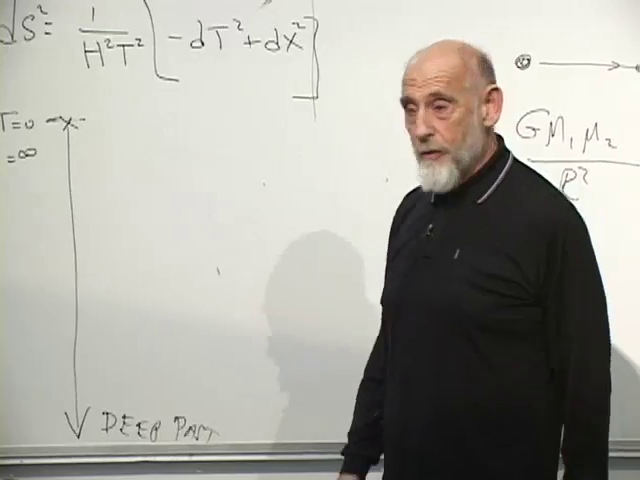
\includegraphics[width=0.86\textwidth]{lecture_08_figure_14.png}
\caption{ヌル条件 \(ds^2=0\) を用いて \(45^\circ\) の光線を回復する時点での共形計量。}
\lectureframe{01:24:05.000}
\end{figure}

\section{ド・ジッター空間におけるアリスとボブ}

アリスを固定された共動位置 \(x=0\) に置く。彼女の世界線は垂直に上昇し、図の上では \(T=0\) で終わるが、彼女の腕時計がそこに到達するには無限の固有時間を要する。その端点から過去向きのヌル光線を引く。それらはアリスが信号を受け取ることのできる最大の領域を境界づける。その外側の事象は永遠に到達不能のままである。

\begin{figure}[htbp]
\centering
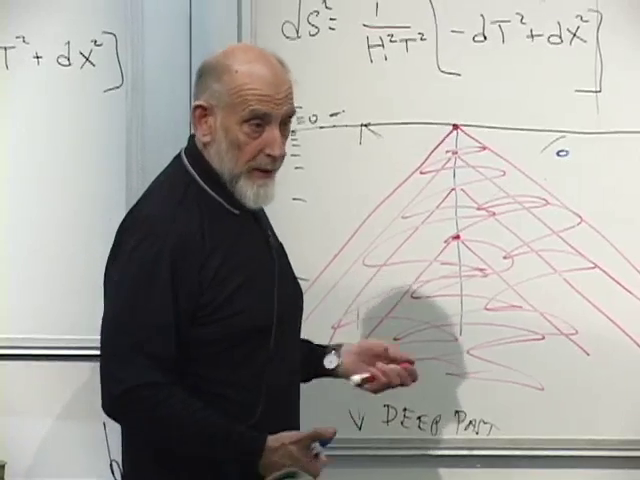
\includegraphics[width=0.88\textwidth]{lecture_08_figure_15.png}
\caption{アリスの限界的な過去光円錐。そのヌル境界が、観測者に依存する彼女のド・ジッター事象の地平面である。}
\lectureframe{01:28:50.000}
\end{figure}

この地平面は私的なものである。異なる観測者は異なる未来の端点を持ち、したがって異なる限界的な過去光円錐を持つ。かつてボブがアリスの因果的領域内にあり、二人がメッセージを交換したとしよう。その後ボブがハッブル流に従ってアリスの地平面を越えると、その越境後に発せられた信号は、アリスがどれほど待っても彼女に届かない。ボブは自分自身の地平面を持ち、やがてアリスからの遅い信号を受け取るという対応する能力を失う。

\begin{figure}[htbp]
\centering
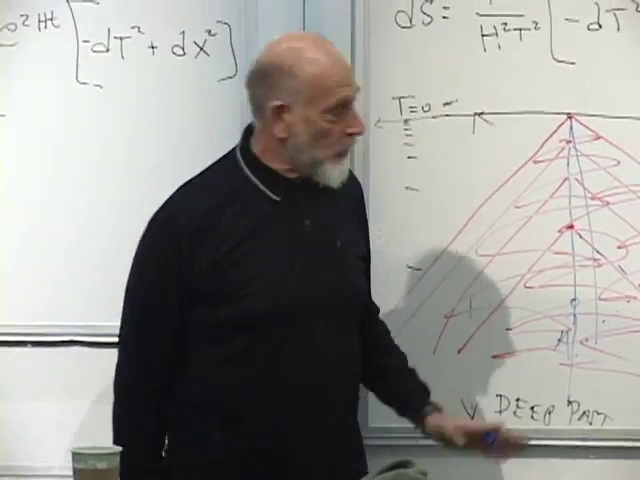
\includegraphics[width=0.88\textwidth]{lecture_08_figure_16.png}
\caption{アリスとボブ、それぞれ異なる因果的境界を持つ。共動するボブは、以前に信号を交換していたとしても、アリスの因果的過去から離れることができる。}
\lectureframe{01:30:20.000}
\end{figure}

アリスとボブが手をつなぐ、あるいはより現実的には固定された固有間隔で束縛され続けるなら、彼らの共動座標の間隔は \(a^{-1}\) として縮む。彼らの曲線は共形図において互いに近づくが、これは彼らの固有距離が消えることを意味しない。増大する共形因子が縮む座標の隔たりを補償し、通信はいつまでも可能なままである。

\begin{classroomqa}
\audiencequestion{地平面が二人を隔てた後、ボブはアリスを同時に見ることができますか。\lecturetimestamp{01:31:43}}
\lecturerresponse{いかなる観測者も、その文字通りの意味で遠方の事象を同時に見ることはない。観測とは常に過去光円錐内の事象についてのものである。より鋭い言明は、地平面の越境後には、もう一方の世界線から新たに発せられた信号は到着し得ないということである。}
\end{classroomqa}

遠い未来の宇宙論的応用では、アリスは我々の束縛された局所的な残存物を表し、ボブはそれぞれの束縛されていない遠方の銀河を表す。銀河はアリスの時計上の有限の瞬間に突然消えるのではない。それらの後の信号はより長い間隔に引き伸ばされ、より長い波長へとずれ、ついには物理的に検出不能になる。

\begin{classroomqa}
\audiencequestion{理論は本当に、遠い未来にはもはや可視の遠方銀河は残らないと言うのですか。\lecturetimestamp{01:33:38}}
\lecturerresponse{束縛されていない銀河は局所観測者の事象の地平面の向こうへと過ぎ去る。それらの最後の可視信号はますます遅延し赤方偏移し、実用上は束縛された局所構造のみが観測可能なまま残る。}
\end{classroomqa}

\section{地平面における赤方偏移}

ボブからの古い光信号が非常に遅い共形時間にアリスに到達する様子を描くことは依然としてでき、それによって彼女が彼を見続けているように見せかけることができる。物理的内容はそれらの信号の間隔とエネルギーにある。ボブの時計の等しい間隔は、アリスの固有時間のますます大きな間隔を隔てて到着する。振動数と光子エネルギーは低下する：
\begin{equation}
\nu_{\rm received}\longrightarrow0,
\qquad
E_{\rm received}=h\nu_{\rm received}\longrightarrow0.
\end{equation}
ボブの像は遅くなり、赤くなり、薄れる。極限の信号は消えゆく有用な情報しか運ばない。

\begin{figure}[htbp]
\centering
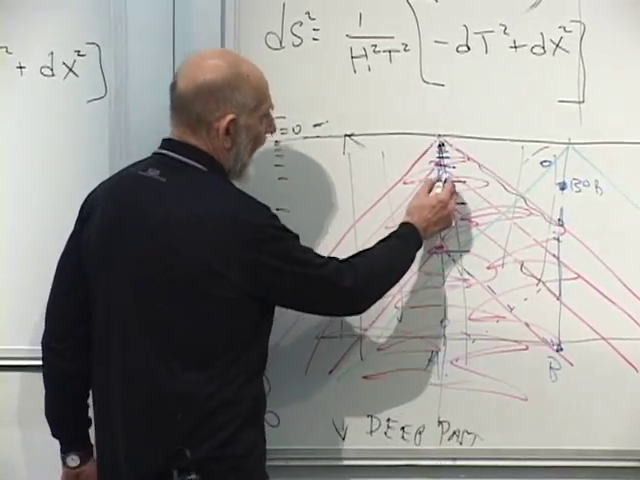
\includegraphics[width=0.89\textwidth]{lecture_08_figure_17.png}
\caption{ド・ジッター地平面の赤方偏移と、ブラックホール地平面のよく知られた外部からの見え方を比較した、後半の板書状態。}
\lectureframe{01:36:20.000}
\end{figure}

\begin{classroomqa}
\audiencequestion{これはブラックホールの場合、すなわち外部の観測者が落下する物体が地平面を越えるのを決して見ないのと同じですか。\lecturetimestamp{01:36:09}}
\lecturerresponse{はい。どちらの場合も、観測者はますます赤方偏移した信号を受け取り、越境が完了するのを直接見ることは決してない。因果図はどの後の放出が決して到着し得ないかを語り、赤方偏移は最後の観測可能な情報がどのように薄れるかを説明する。}
\end{classroomqa}

この類推は温度についての問いを促す。

\begin{classroomqa}
\audiencequestion{アリスはどうやって地平面のすぐ上の温度を測定できるのだろうか。\lecturetimestamp{01:39:34}}
\lecturerresponse{操作上は、ケーブルで温度計を降ろし、地平面を越えないように保ち、そして引き戻せばよい。ド・ジッター観測者は宇宙論的地平面の近くで同様の実験を想像できる。量子論では地平面は熱いが、本講義は古典幾何学で止まり、その計算は先送りにする。}
\end{classroomqa}

ここではド・ジッター温度の公式は導出されない。ホーキング放射は、この古典的描像に対する量子補正の予告としてのみ登場する。

\section{固定された地平面半径}

共形図は元の時間座標に翻訳し直すことができる。固定された座標間隔にある2つの共動点は
\begin{equation}
D(t)=e^{Ht}\lvert\Delta x\rvert,
\end{equation}
を満たすので、それらの固有距離は指数的に増大する。

\begin{classroomqa}
\audiencequestion{同じ運動は、変換前の元の時間座標ではどのように見えるだろうか。\lecturetimestamp{01:41:14}}
\lecturerresponse{固定された共動座標に対して、空間計量全体が\(e^{2Ht}\)とともに増大する。したがって固有間隔は\(e^{Ht}\)のように増大する。座標変換を元に戻すと、その膨張が明示的になる。}
\end{classroomqa}

地平面は異なる振る舞いをする。なぜなら、アリスからの共動座標距離は固定されていないからである。\(T=0\)で終わる\(45^\circ\)のヌル線から、一定の\(T<0\)のスライス上での地平面距離は
\begin{equation}
\Delta x_H=-T=\frac{1}{H}e^{-Ht}.
\label{eq:l08-coordinate-horizon}
\end{equation}
であり、スケール因子を掛けると
\begin{equation}
D_H(t)=a(t)\Delta x_H
=e^{Ht}\frac{e^{-Ht}}{H}
=\frac{1}{H}.
\label{eq:l08-fixed-horizon}
\end{equation}
となる。単位を戻すと、\(D_H=c/H\)である。座標間隔は縮み、計量スケールは成長し、それらの積は一定に保たれる。

\begin{classroomqa}
\audiencequestion{時間が経つにつれて、アリスから地平面までの距離は増大するだろうか、縮小するだろうか、それとも同じままであるだろうか。\lecturetimestamp{01:42:42}}
\lecturerresponse{同じままである。その座標距離は縮む一方で共形因子が成長し、\(c=1\)とする単位で固有地平面半径は\(H^{-1}\)に固定されたままである。}
\end{classroomqa}

\begin{figure}[H]
\centering
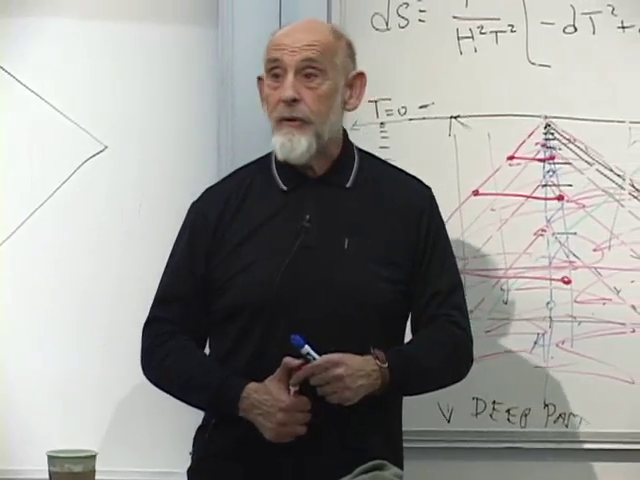
\includegraphics[width=0.90\textwidth]{lecture_08_figure_18.png}
\caption{最終的な板書の状態：連続する水平スライスでは、地平面までの座標距離は縮小するが、固有距離は同じである。}
\lectureframe{01:43:20.000}
\end{figure}

\begin{classroomqa}
\audiencequestion{古い像が決して完全には消えないために、アリスは過去が地平面に投影されたものを見続けるのだろうか。\lecturetimestamp{01:43:45}}
\lecturerresponse{古典的には、それらの像は、無限に続く赤方偏移によってますます検出しにくくなるという極限的な意味でのみ持続する。この記述は、地平面に付随するホーキング放射を省いており、それが量子論的記述を変更するだろう。}
\end{classroomqa}

したがって講義は、正確な境界で終わる。真空エネルギーが指数的膨張を生み、指数的膨張が固定された観測者依存の事象の地平面を生み、そしてその地平面の近くの信号は振動数がゼロになるまで追いやられた。地平面の温度とホーキング放射は次に来るものに属する。ススキンドが言うように、我々が互いの地平面を横切らないと仮定すれば、次の講義でまた会おう。

\chapter{ド・ジッター地平線と宇宙論的確率}

\lectureoverview{地平線は単なる因果的境界ではない。定常観測者にとってそれは熱系である。地平線から固有距離\(\rho\)の位置に保持された温度計は\(1/(2\pi\rho)\)程度の温度を示すが、重力赤方偏移により遠方で見られる放射ははるかに低温になる。このブラックホールの教訓をド・ジッター空間に持ち込み、固定された地平線半径\(H^{-1}\)を導出し、観測者の静的パッチ計量を書き下す。講義の後半では熱力学をその落ち着かない帰結まで追う。有限なド・ジッターエントロピー、ポアンカレ再帰、ボルツマン脳、永久インフレーション、そして測度問題である。最後の議論では、弦理論の厳密な超対称構造と、我々の世界を記述するかもしれない依然として未知の枠組みとを区別する。}

\section{地平線が熱いとはどういうことか}

本講義の前に、その夜の方向性を決める問いから始める。

\begin{classroomqa}
\audiencequestion{宇宙論的地平線にはブラックホールは存在しない。それにもかかわらず、どのような機構によってそれは熱くなりうるのか。\lecturetimestamp{00:00:17}}
\lecturerresponse{機構はブラックホール地平線の場合と同じである。有用な問いは操作的である。地平線近くに保持された温度計は何を記録するのか、そして地平線から遠く離れた観測者にはどのような放射が届くのか。}
\end{classroomqa}

最初の実験は局所的である。任意の滑らかな非極端地平線から固定された固有距離\(\rho\)の位置に温度計を保持する。地平線に十分近づくと、幾何学は普遍的なリンドラー形式を持ち、温度計は次を読み取る。
\begin{equation}
T_{\rm local}(\rho)\simeq \frac{1}{2\pi\rho}
\label{eq:l09-local-temperature}
\end{equation}
単位は\(\hbar=c=k_B=1\)とする。定数を復元すると次を得る。
\begin{equation}
k_B T_{\rm local}(\rho)\simeq \frac{\hbar c}{2\pi\rho}.
\end{equation}
\(\rho\to0\)における発散は、落下する観測者が通常の物質的な炉に遭遇することを意味しない。それは、地平線のすぐ外側にとどまり、したがってますます激しく加速しなければならない観測者によって割り当てられる温度である。

冒頭の会話はまた、混同されやすい三つの概念を区別する。エネルギー、温度、エントロピーである。

\begin{classroomqa}
\audiencequestion{光子をブラックホールに送り込んだ場合、依然として同じエントロピーを測定するのか、それともエネルギーだけが変化するのか。\lecturetimestamp{00:01:22}}
\lecturerresponse{光子が地平線の背後で到達不能になると、追加の情報が隠されたことになる。ここで用いられる単純化されたビットの言葉では、一つの光子は一つの追加ビットを隠し、それによってエントロピーを増加させうる。エネルギー、温度、エントロピーは関係しているが、互換ではない。}
\end{classroomqa}

\editorialnote{物理的なブラックホールに対して、エントロピー変化は熱力学的に\(dS=dE/T_H\)によって固定される。エネルギーによらずすべての光子について普遍的に1ビットであるわけではない。1ビットという記述は本講義の情報理論的理想化である。}

地平線近傍領域は高周波の量子揺らぎを絶えず放出し再吸収している。地平線は、定常観測者にとってそれらの揺らぎを熱的にする。しかしこれは直ちに一つの難問を提起する。もしその領域が任意に熱いなら、なぜ遠方の観測者は任意に高エネルギーの光子によって目をくらまされないのか。

\section{赤方偏移とホーキング温度}

通常の熱い壁は、我々がそこから遠く離れて立っていても、高周波放射の源であり続ける。地平線は、その放射が重力赤方偏移を経て登らなければならない点で異なる。光子の速さは\(c\)のままであり、減少するのはそのエネルギーである。
\begin{equation}
E=\hbar\omega,
\qquad
\omega_{\rm received}<\omega_{\rm emitted}.
\end{equation}
講義で用いられたチョークの比喩は、この点までは有用である。投げ上げられた石は上昇するにつれて減速するが、光子は光速を保ちながらその振動数とエネルギーが減少する。

シュヴァルツシルトブラックホールについて、無限遠の観測者が測定する温度は次である。
\begin{equation}
T_H=\frac{1}{8\pi M}
\label{eq:l09-hawking-natural}
\end{equation}
単位は\(G_N=\hbar=c=k_B=1\)とする。通常の単位では、
\begin{equation}
T_H=\frac{\hbar c^3}{8\pi G_N M k_B}.
\label{eq:l09-hawking-full}
\end{equation}

\begin{figure}[htbp]
\centering
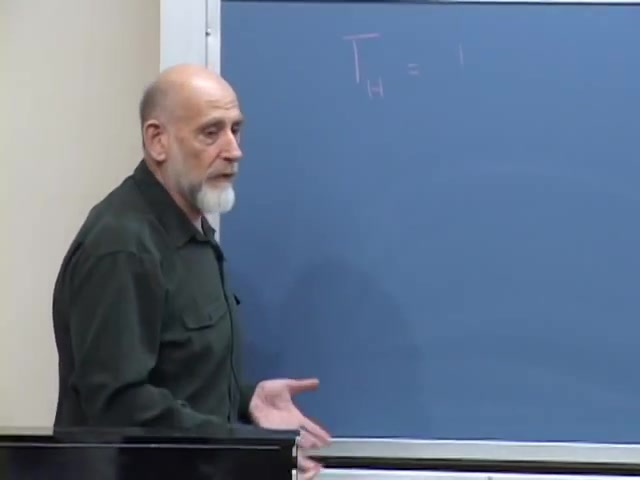
\includegraphics[width=0.68\textwidth]{lecture_09_figure_02.png}
\caption{自然単位でのホーキング温度\(T_H=1/(8\pi M)\)。}
\lectureframe{00:08:12}
\end{figure}

より大きなブラックホールはより低温である。講義ではこれを、典型的な光子を逆向きにたどることで説明する。熱的光子は特性エネルギー\(E_\gamma\sim T_H\)を持つ。\(M^{-1}\)程度のエネルギーで無限遠に到達する光子は、地平線近くを出発したときにはるかに大きな局所エネルギーを持っていた。地平線近傍の層と無限遠との間の赤方偏移は、より大きなブラックホールに対してより厳しくなり、より低い漸近温度を残す。

\begin{classroomqa}
\audiencequestion{もしシュヴァルツシルト時間が地平線で凍結するなら、もともと落下してブラックホールを形成した光子を追うべきではないのか。\lecturetimestamp{00:04:19}}
\lecturerresponse{温度の問題については、外向きに放出された光子を追えばよい。それらは非常に高い局所振動数で出発し、外へ登る間にエネルギーを失い、ホーキング放射として到達する。もともと落下した光子の運命は、別個の情報の問題である。}
\end{classroomqa}

\section{プランク層と引き伸ばされた地平線}

式~\eqref{eq:l09-local-temperature}の局所的な関係はどこまで信頼できるだろうか。この講義では、半古典的記述における意味を持つ最短距離としてプランク長を採用する。このことは、数学的な地平面のすぐ外側、およそプランク長一つ分の薄い層がプランクスケールの揺らぎで満たされていることを示唆する。それは絶えず放出と吸収を行っている。

放出された量子のほとんどは脱出しない。外向きの非常に狭い円錐へ向かうものだけが、落下して戻ることを免れる。一般的な角度で放たれた量子は地平面へ戻る。外向きと内向きの励起が衝突し、対やその他の粒子を生成する。この意味で、定常的な記述は極めて高温の物質の薄い殻を含んでいる。

\begin{figure}[htbp]
\centering
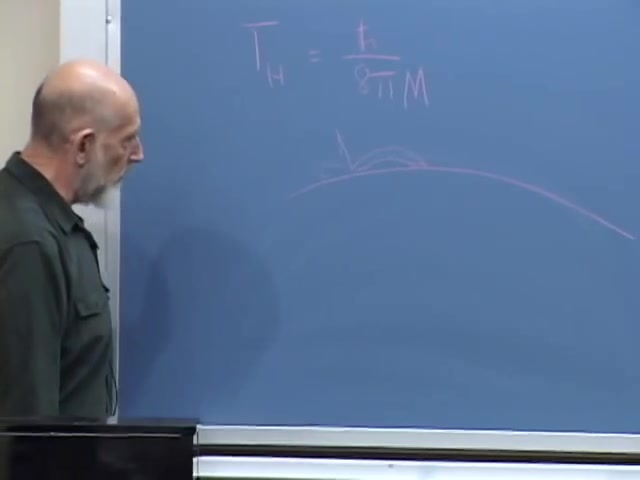
\includegraphics[width=0.74\textwidth]{lecture_09_figure_03.png}
\caption{地平面近傍の放射に対する狭い脱出円錐。局所的に放出された量子のほとんどは地平面へ戻る。}
\lectureframe{00:11:38}
\end{figure}

相補的な時空描像がある。地平面から離れては、仮想的な揺らぎは模式的に短い閉じたループで表されることがある。粒子・反粒子の励起が現れ、漸近状態になり得る前に消えるのである。地平面の近くでは、揺らぎは因果的境界をまたぐことができる。外部の観測者にとって、外側の部分は地平面から放出され、後に再吸収される粒子のように見える。ごくわずかな割合が脱出し、ホーキング放射となる。

\begin{classroomqa}
\audiencequestion{外部の図において、そのような揺らぎは\(t=-\infty\)から\(t=+\infty\)まで伸びるのか。\lecturetimestamp{00:15:00}}
\lecturerresponse{厳密な古典的地平面は、その特異に見える記述をもたらす。実際には、それを伸長地平面、すなわちおよそプランク長一つ分だけ外側にある時間的曲面で置き換える。すると放出と再吸収は有限の外部時間で起こる。}
\end{classroomqa}

\begin{figure}[htbp]
\centering
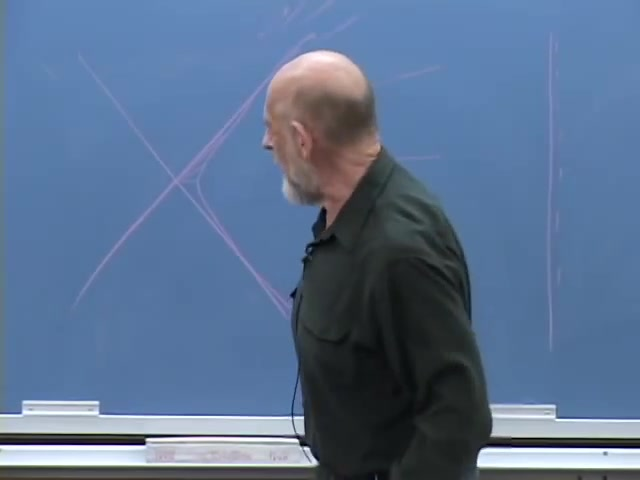
\includegraphics[width=0.72\textwidth]{lecture_09_figure_04.png}
\caption{古典的地平面と、外部記述で用いられる近傍の伸長地平面。}
\lectureframe{00:15:52}
\end{figure}

伸長地平面は新しい不変な境界ではない。それは半古典的幾何学が信頼できなくなる場所に置かれた有効な曲面である。物質および幾何学自体の量子揺らぎが、厳密な位置をプランクスケールでぼかす。この構成は、その不確定性を、外部記述が有限に保たれる曲面上にまとめ上げる。

この局所的な議論のどこにも、地平面がブラックホールに属するのか、加速する宇宙に属するのかを知る手がかりはない。それがド・ジッター空間への橋渡しである。

\section{膨張座標におけるド・ジッター空間}

正式な講義は、ド・ジッター時空の空間的に平坦なスライスから始まる。
\begin{equation}
ds^2=-dt^2+e^{2Ht}d\mathbf{x}^2,
\qquad
d\mathbf{x}^2=dx^2+dy^2+dz^2.
\label{eq:l09-flat-slicing}
\end{equation}
定数\(H\)はド・ジッター膨張率である。この因子が\(e^{2Ht}\)として現れるのは、計量が距離の二乗を測るからである。固定された座標間隔は物理的長さ
\begin{equation}
D(t)=e^{Ht}\lvert\Delta\mathbf{x}\rvert.
\end{equation}
を持つ。

\begin{figure}[htbp]
\centering
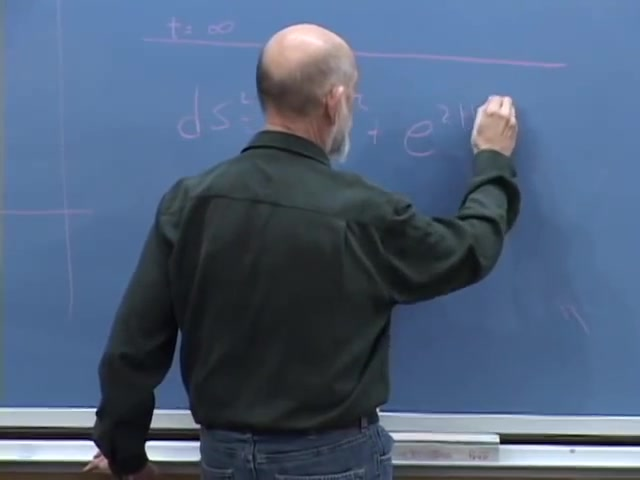
\includegraphics[width=0.78\textwidth]{lecture_09_figure_05.png}
\caption{平坦座標における指数的に膨張するド・ジッター計量。}
\lectureframe{00:18:50}
\end{figure}

これらの座標は膨張を明瞭にするが、未来の無限遠をページのはるか上方に置く。それを黒板に持ち込むために、共形時間を導入する。
\begin{equation}
\eta=-\frac{1}{H}e^{-Ht},
\qquad
-\infty<\eta<0.
\label{eq:l09-conformal-time}
\end{equation}
すると
\begin{equation}
dt=\frac{d\eta}{-H\eta},
\qquad
e^{Ht}=-\frac{1}{H\eta},
\end{equation}
であり、式~\eqref{eq:l09-flat-slicing}は
\begin{equation}
ds^2=\frac{1}{H^2\eta^2}
\left(-d\eta^2+d\mathbf{x}^2\right).
\label{eq:l09-conformal-metric}
\end{equation}
となる。\(t\to+\infty\)のとき、\(\eta\to0^{-}\)である。無限の固有時間が、有限の水平線\(\eta=0\)へ圧縮されたのである。

\editorialnote{時間の変換は黒板に書いている間に何度か修正される。式~\eqref{eq:l09-conformal-time}が整合的な形である。初期の宇宙時間は\(\eta\to-\infty\)へ写り、未来の無限遠は\(\eta\to0^{-}\)へ写る。}

\begin{figure}[htbp]
\centering
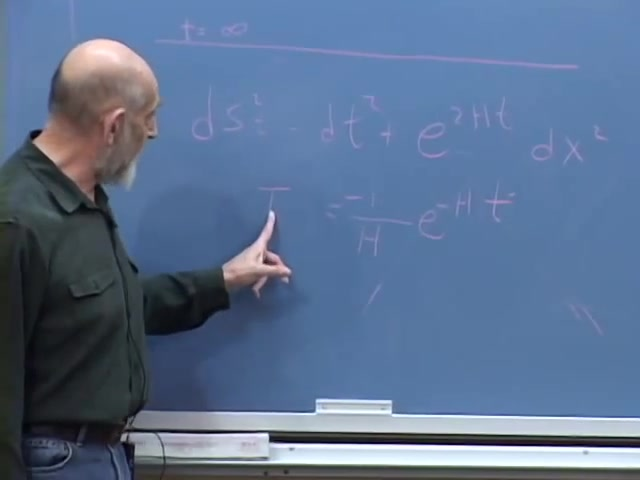
\includegraphics[width=0.82\textwidth]{lecture_09_figure_06.png}
\caption{共形時間の変換と共形的に平坦な計量。}
\lectureframe{00:21:24}
\end{figure}

共形因子は時間項と空間項の両方に掛かるので、ヌル方向を変えない。動径方向の光線に対して
\begin{equation}
ds^2=0
\quad\Longrightarrow\quad
-d\eta^2+dx^2=0
\quad\Longrightarrow\quad
\frac{dx}{d\eta}=\pm1.
\label{eq:l09-null-rays}
\end{equation}
したがって光は共形図において\(45^\circ\)で進む。これが座標変換が有用である理由である。因果的可到達性が見えるようになるのである。

\section{一人の観測者の因果的パッチ}

世界線が無限の固有時間にわたって続く観測者を想像しよう。コンパクト化された図では、それは\(\eta=0\)上の一点で終わる。その観測者が受け取ることのできるあらゆる信号は、その端点の過去光円錐の内側にある。円錐の外側の事象は、観測者がどれほど長く待っても、その観測者と決して通信できない。

\begin{figure}[htbp]
\centering
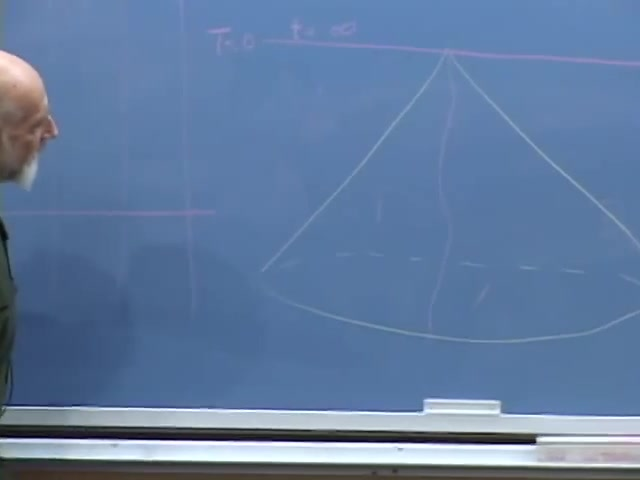
\includegraphics[width=0.78\textwidth]{lecture_09_figure_07.png}
\caption{共形ド・ジッター座標における観測者の極限的な過去光円錐。}
\lectureframe{00:24:38}
\end{figure}

第二の観測者は異なる円錐を持つ。二つの可到達領域は重なるが、どちらも時空全体ではない。以下の議論では第一の観測者の視点を採用し、その過去光円錐をその観測者の因果的パッチと呼ぶ。

図はパッチが未来に向かって縮むように見えるが、座標幅は固有距離ではない。一定の\(\eta\)スライス上で、\(x=0\)にいる観測者と\(x=\Delta x\)にある地平線との間の物理的距離の二乗は
\begin{equation}
D^2=\frac{(\Delta x)^2}{H^2\eta^2}.
\label{eq:l09-horizon-distance-start}
\end{equation}
である。地平線は\(\eta=0\)で終わる\(45^\circ\)のヌル線であるから、
\begin{equation}
\Delta x=\lvert\eta\rvert.
\end{equation}
となる。代入すると
\begin{equation}
D_{\rm hor}^2=\frac{1}{H^2},
\qquad
D_{\rm hor}=\frac{1}{H}.
\label{eq:l09-horizon-radius}
\end{equation}
が得られる。座標間隔は縮むが、共形因子はちょうど補償する分だけ大きくなる。固有地平線半径は一定である。

\begin{figure}[htbp]
\centering
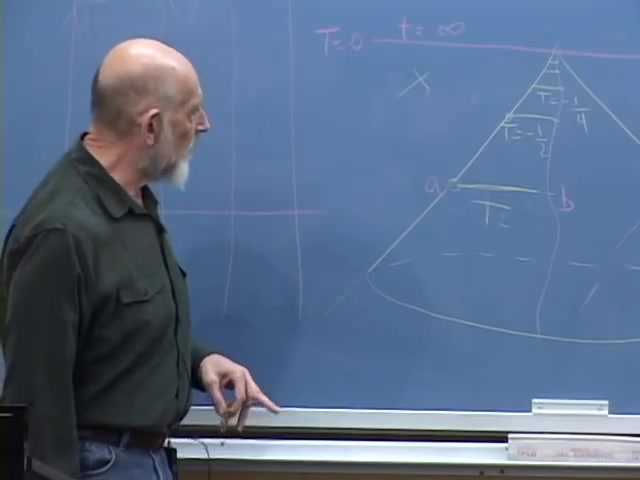
\includegraphics[width=0.80\textwidth]{lecture_09_figure_08.png}
\caption{縮む座標間隔を固定された固有距離\(H^{-1}\)に変換する板書の導出。}
\lectureframe{00:28:42}
\end{figure}

\section{静的パッチ}

地平線半径が固定されていることは、中心の観測者に適合した座標を示唆する。座標変換を導出することなく、講義は結果を次のように書く：
\begin{equation}
ds^2=
-\left(1-H^2r^2\right)d\tau^2
+\frac{dr^2}{1-H^2r^2}
+r^2d\Omega_2^2.
\label{eq:l09-static-patch}
\end{equation}
係数は\(\tau\)ではなく\(r\)に依存する。このチャートは観測者の静的パッチを覆い、
\begin{equation}
0\le r<\frac{1}{H}.
\end{equation}

\begin{figure}[htbp]
\centering
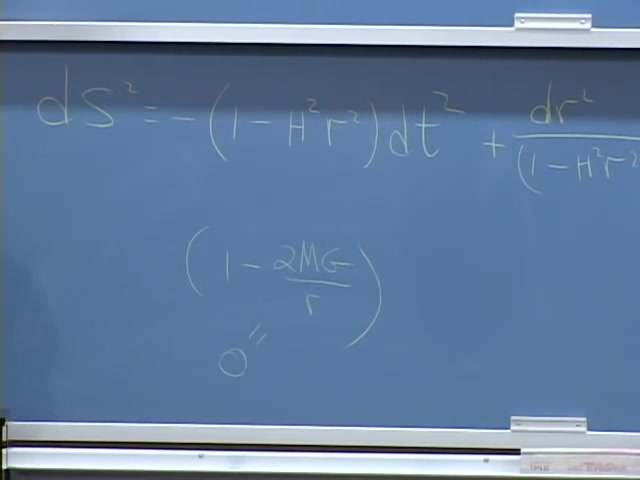
\includegraphics[width=0.88\textwidth]{lecture_09_figure_09.png}
\caption{ド・ジッター静的パッチ計量と、シュヴァルツシルト因子との比較。}
\lectureframe{00:34:22}
\end{figure}

シュヴァルツシルトとの類似は即座に明らかである：
\begin{equation}
f_{\rm dS}(r)=1-H^2r^2,
\qquad
f_{\rm Schw}(r)=1-\frac{2G_NM}{r}.
\end{equation}
いずれの場合も、静的座標の地平線は\(f(r)=0\)となる場所に現れる。ド・ジッターの場合、
\begin{equation}
1-H^2r^2=0
\quad\Longrightarrow\quad
r_H=H^{-1}.
\end{equation}
このチャートはそこで特異であり、ちょうどシュヴァルツシルト座標がブラックホールの地平線で特異であるのと同じである。それにもかかわらず、大域的な幾何学は重要な点で異なる。ブラックホールの観測者は外側に立って内側を見る。ド・ジッターの観測者は内側に立って外側を見る。

\begin{classroomqa}
\audiencequestion{自由に放たれた粒子が指数関数的に膨張する宇宙で互いに離れていくとき、幾何学が静的でありうるのはなぜか。\lecturetimestamp{00:36:06}}
\lecturerresponse{静的とは、すべての粒子が固定されているという意味ではない。計量の係数と、繰り返された実験の結果が開始時刻に依存しないという意味である。今、二つの粒子を放てばそれらは加速しながら離れていく。同じ実験を後で繰り返せば、同じ運動が起こる。}
\end{classroomqa}

\begin{classroomqa}
\audiencequestion{離れていく二つの粒子は互いに赤方偏移を見るか。\lecturetimestamp{00:38:34}}
\lecturerresponse{はい。観測者に適合した計量が時間に依存しなくても、それらの間隔が増大することは相対的な赤方偏移を生む。}
\end{classroomqa}

\section{内側から見た温度}

シュヴァルツシルト空間とド・ジッター空間の地平線近傍の構造は局所的に等価である。したがってド・ジッター地平線は熱的量子を放出し再吸収する。まれな光子は中心の観測者へ内向きに伝播し、静的パッチのポテンシャルを登るにつれてエネルギーを失う。中心で測定されるギボンズ--ホーキング温度は
\begin{equation}
T_{\rm dS}=\frac{H}{2\pi}
\label{eq:l09-de-sitter-temperature}
\end{equation}
であり、自然単位を用いている。半径\(r\)にある静止した温度計はトールマン赤方偏移された値
\begin{equation}
T_{\rm local}(r)=
\frac{T_{\rm dS}}{\sqrt{1-H^2r^2}},
\label{eq:l09-tolman}
\end{equation}
を読み取り、これは\(r\to H^{-1}\)として発散し、地平線近くでは式~\eqref{eq:l09-local-temperature}に帰着する。

\editorialnote{講義は式~\eqref{eq:l09-de-sitter-temperature}と\eqref{eq:l09-tolman}を明示的に書く代わりに、地平線距離と赤方偏移からスケールを導出する。それらはその議論の標準的な規格化を述べている。}

観測された晩期の加速に対して、講義は期間の推定値
\begin{equation}
H^{-1}\sim 20\times10^9\ {\rm light\ years}.
\label{eq:l09-lecture-horizon-estimate}
\end{equation}
を用いる。すると典型的な地平線光子は数十億光年に匹敵する波長を持つ。これはマイクロ波背景放射ではない。はるかに低温である。

操作的思考実験は宇宙論的スケールの釣り竿である。アリスは\(r=0\)にとどまり、データも伝送する非常に長い糸に温度計を取り付け、宇宙の斥力に計器を外側へ運ばせる。彼女はそれを地平線のすぐ手前で止め、信号が戻るのを待つと、大きな局所温度を見出す。中心で彼女のそばにある温度計は微小な値\(H/(2\pi)\)を読み取る。一つの地平線が両方の読みを支えるのは、それらが異なる重力ポテンシャルで行われるからである。

\section{地平線の横断}

古典的な外側の記述は、よく知られたブラックホールの話に似ている。中心にいるボブはアリスが遠ざかるのを見る。彼女の信号はますます赤方偏移し、ますますゆっくりと到着する。彼女は地平線に押しつぶされて見え、最終的に薄れていく。後から来る旅行者ジェーンは、境界近くの堆積層の中のもう一つのより薄い層として現れる。

\begin{classroomqa}
\audiencequestion{我々の視点から、物体はかつて宇宙の地平線を通り抜けるのか。\lecturetimestamp{00:45:30}}
\lecturerresponse{静的観測者の古典的記述では通り抜けない。それらの信号は赤方偏移して薄れ、見かけの位置は地平線に近づく。しかし、それら自身の自由落下の記述では、それらは局所的に特異な面に出会うことなく横断する。}
\end{classroomqa}

\begin{classroomqa}
\audiencequestion{地平線が熱いのは、そこを越えずに近くにとどまる観測者にとってだけなのだろうか？落下する観測者は、ただ通過するだけで焼かれてしまうわけではないのだろう？\lecturetimestamp{00:48:27}}
\lecturerresponse{アリスは自身の座標系では滑らかに越えていく。極端な温度は静止した記述に属する。ボブがアリスを地平線にどこまでも近づけて分解しようと固執するなら、彼はますます短い波長でアリスを照らさなければならない。その試みられたハイゼンベルク顕微鏡は、観測しようとするものを焼くのに十分なエネルギーを注ぎ込むことになる。}
\end{classroomqa}

これは二つの局所的な事象の間の矛盾ではない。静止した観測者と落下する観測者は根本的に異なる測定を用いている。地平線相補性は、一方の観測者が重複した情報を直接比較することを許さずに、どのようにして両方の記述が妥当でありうるかを問うものである。

\section{真空の斥力のニュートン模型}

この時点で、学生がブラックホールの重力井戸に代わるものは何かと尋ねる。サスキンドはニュートン模型を構成することで答える。\(\phi\) を重力ポテンシャルとすると、試験粒子の加速度は
\begin{equation}
\mathbf{a}=-\boldsymbol{\nabla}\phi.
\end{equation}
通常の非相対論的物質に対しては、ポアソン方程式は
\begin{equation}
\nabla^2\phi=4\pi G_N\rho.
\label{eq:l09-poisson}
\end{equation}

\begin{classroomqa}
\audiencequestion{ブラックホールの効果がその重力井戸から来るのなら、ド・ジッター空間における対応する源は何か？\lecturetimestamp{00:49:36}}
\lecturerresponse{真空エネルギー自体が空間的に一様な重力源を与える。ニュートン的記述では、それは \(1/r\) の井戸ではなく二次のポテンシャルを生じる。}
\end{classroomqa}

\begin{figure}[htbp]
\centering
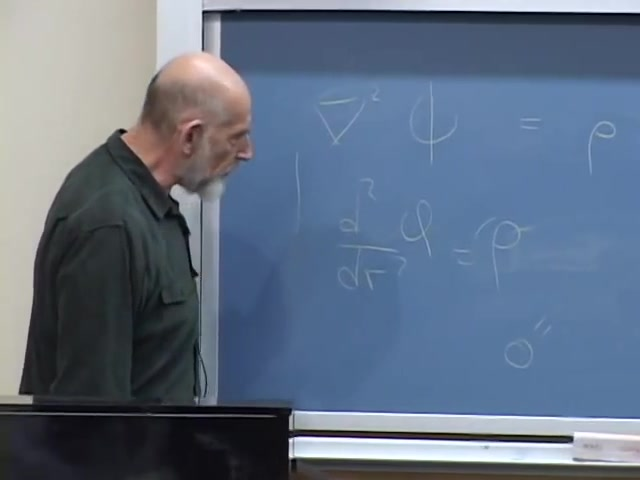
\includegraphics[width=0.78\textwidth]{lecture_09_figure_10.png}
\caption{ポアソン方程式と、講義で用いられた模式的な動径方向二階微分の形。}
\lectureframe{00:51:38}
\end{figure}

板書では規格化、球面測度の項、圧力、そして当初は全体の符号さえも省かれ、演習は
\begin{equation}
\frac{d^2\phi}{dr^2}\sim H^2.
\end{equation}
に還元される。本質的な推論は、一定の源が二次関数を与えるということである。ド・ジッター斥力に必要な符号をとると、
\begin{equation}
\phi_{\rm dS}(r)=-\frac{1}{2}H^2r^2,
\qquad
a_r=-\frac{d\phi_{\rm dS}}{dr}=H^2r.
\label{eq:l09-de-sitter-potential}
\end{equation}
加速度は外向きを向き、距離に比例して増大する。\(\ddot r=H^2r\) を解くと
\begin{equation}
r(\tau)=A e^{H\tau}+B e^{-H\tau},
\end{equation}
となり、増大する枝が指数的な分離を再現する。

\begin{figure}[htbp]
\centering
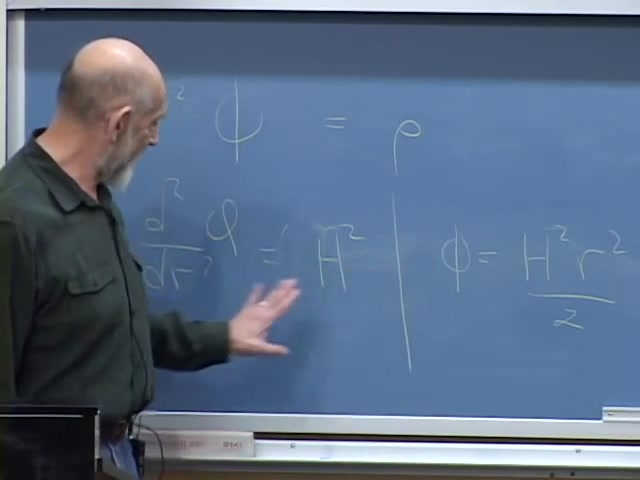
\includegraphics[width=0.76\textwidth]{lecture_09_figure_11.png}
\caption{一様な源の方程式と、二次のド・ジッターポテンシャル。}
\lectureframe{00:53:32}
\end{figure}

\editorialnote{一般相対論では、一様な流体の弱場加速度は \(\rho+3p\) に依存し、\(\rho\) だけには依存しない。真空エネルギーは \(p=-\rho\) をもつので、\(\rho+3p=-2\rho\) となり、加速度は斥力的である。式~\eqref{eq:l09-de-sitter-potential} は正しく規格化されたド・ジッターの結果であり、板書の計算は意図的に二次の依存性と符号のみを追っている。}

中心に通常の質量 \(M\) を置く。定性的なポテンシャルは
\begin{equation}
\phi(r)=-\frac{G_NM}{r}-\frac{1}{2}H^2r^2,
\label{eq:l09-combined-potential}
\end{equation}
となり、動径方向の加速度は
\begin{equation}
a_r=-\frac{G_NM}{r^2}+H^2r.
\end{equation}
である。小さい \(r\) では局所的な引力が勝ち、大きい \(r\) では真空の斥力が勝つ。それらの釣り合いは
\begin{equation}
r_\ast=\left(\frac{G_NM}{H^2}\right)^{1/3}.
\label{eq:l09-turnaround}
\end{equation}
で起こる。これは講義におけるポテンシャルの極大のきれいな版である。近くの重力束縛系がまとまったままでいられる一方、十分に遠い銀河が加速して遠ざかる理由を定性的に説明する。

\begin{figure}[htbp]
\centering
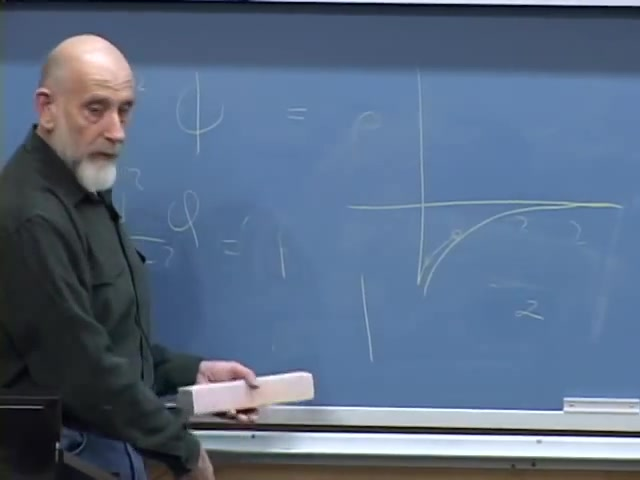
\includegraphics[width=0.78\textwidth]{lecture_09_figure_12.png}
\caption{通常の \(1/r\) 引力と、逆さまの二次のド・ジッターポテンシャルとの組み合わせ。}
\lectureframe{00:58:20}
\end{figure}

\begin{classroomqa}
\audiencequestion{通常の力は依然として重要か、それとも真空の斥力が最終的にあらゆる物質の島を引き裂くのか？\lecturetimestamp{00:57:29}}
\lecturerresponse{すべての力を含めなければならない。十分に小さいスケールでは、電磁気的な束縛と局所的な重力が支配する。真空の斥力が重要になるのは、\(H^{-1}\) と、束縛された質量に応じた釣り合いのスケールによって定まる巨大な距離を越えてのみである。}
\end{classroomqa}

\section{一つの源、いくつかの名前}

ここで議論は用語をめぐって小休止する。真空エネルギー、宇宙定数、暗黒エネルギーは、用いられている模型における三つの加算的な実体ではない。それらは同じ \(w=-1\) の源についての三つの記述である。アインシュタイン方程式における定数項、真空のローレンツ不変なエネルギー密度、あるいは後期の加速を駆動する成分について語ることができる。

\begin{classroomqa}
\audiencequestion{一様なニュートン的源と量子真空エネルギーは、別々の効果として両方存在するのか？\lecturetimestamp{00:59:14}}
\lecturerresponse{いいえ。一様な密度は同じ源のニュートン模型である。真空エネルギー、宇宙定数、そしてこの講義では暗黒エネルギーは、一つの物理的成分を指す。}
\end{classroomqa}

\begin{classroomqa}
\audiencequestion{それでは、同じ現象が古典的な記述と量子的な記述の両方をもつことになるのでしょうか。\lecturetimestamp{01:00:32}}
\lecturerresponse{その微視的起源は量子力学的でありうる。ちょうど電子の質量の一部が量子的起源をもつように。有効エネルギー密度がわかれば、それは通常の源として古典的な重力方程式に入る。観測された値の究極の起源はわかっていない。}
\end{classroomqa}

プランク単位では、観測されている真空エネルギー密度は極めて小さく、
\begin{equation}
\rho_\Lambda\sim10^{-123}\rho_{\rm Pl},
\label{eq:l09-planck-smallness}
\end{equation}
プランク密度に用いる規約にもよるが、その程度である。この小さな数が宇宙定数問題である。また、それゆえに地平線がこれほど大きいのである。4次元では、
\begin{equation}
H^2=\frac{8\pi G_N}{3}\rho_\Lambda,
\qquad
r_H=H^{-1}.
\end{equation}
もし\(H\)がより大きければ、地平線はより小さくなり、中心のド・ジッター温度はより高くなり、斥力的加速度\(H^2r\)はより強くなるであろう。

\begin{classroomqa}
\audiencequestion{この微小な宇宙定数は、プランク定数や量子ゆらぎと関係しているのでしょうか。\lecturetimestamp{01:03:27}}
\lecturerresponse{きれいな比較には無次元のプランク単位が用いられ、そこでは\(G_N=\hbar=c=1\)である。その単位では、真空密度は自然なプランク密度よりおよそ\(123\)桁小さい。この階層性を説明することは、基礎物理学の中心的難問の一つである。}
\end{classroomqa}

\begin{classroomqa}
\audiencequestion{真空エネルギーは厳密に一定の宇宙定数でなければならないのでしょうか。加速成分が減少し、最終的にゼロに落ち着くことはありえませんか。\lecturetimestamp{01:04:52}}
\lecturerresponse{それは論理的に可能な代替案である。すなわち、動的な暗黒エネルギー場が時間とともに変化しうる。講義では一定の場合を採用している。それは、当時利用可能な観測が宇宙定数に近い振る舞いをますます支持していたからであり、あらゆる代替案が不可能であると証明されていたからではない。}
\end{classroomqa}

\section{遠い未来の天文学}

漸近的にド・ジッター的な宇宙では、重力で束縛されていない構造はやがて観測者の地平線を越える。宇宙マイクロ波背景放射は検出限界以下に赤方偏移する。遠方の銀河は消える。生き残った天文学者は、そうでなければ暗い領域の中に、合体した局所的な重力の島だけを見るかもしれない。

\begin{classroomqa}
\audiencequestion{望遠鏡がなければ、遠方の銀河が消えたことに誰か気づくことさえあるでしょうか。\lecturetimestamp{01:06:17}}
\lecturerresponse{おそらくないであろう。深刻な問題はもっと深い。高度な観測機器があっても、未来の観測者は、今日われわれが膨張を推測するもととなる遠方のトレーサーやマイクロ波背景放射を欠くかもしれない。}
\end{classroomqa}

そのとき、古い島宇宙像が説得力をもつように見えるかもしれない。オルバースのパラドックスは別の結論を強いることはないであろう。なぜならそれは、無限で静的で一様な発光源の集団を仮定しているからであり、未来の観測者は局所的な島の有限個の恒星だけを見るであろう。暗黒エネルギーが空虚な空間から絶えず代わりの銀河を作り出すわけではない。

厳密なド・ジッター空間における地平線は、局所的な銀河の周りで縮まない。その物理的半径は\(H^{-1}\)のままであり、銀河よりはるかに大きい。消えるのは、その固定された因果的境界の向こうへ運ばれた束縛されていない物質である。

\begin{classroomqa}
\audiencequestion{銀河から放出された恒星は、大規模な幾何学を検出するための試験体として役立ちうるでしょうか。\lecturetimestamp{01:11:25}}
\lecturerresponse{しばらくの間は、役立つ。放出された天体や長基線の光信号は幾何学を探ることができる。しかし、その効果が有意になるのは10億光年の相当な割合程度の距離にわたってのみであり、したがってその実験には宇宙論的な時間がかかるであろう。}
\end{classroomqa}

\begin{classroomqa}
\audiencequestion{遠方の地平線がすでに宇宙の大部分をわれわれから隠しているのではないと、どうしてわかるのでしょうか。\lecturetimestamp{01:11:45}}
\lecturerresponse{われわれはすでに十分な数の銀河、赤方偏移、背景放射を見ており、膨張を測定し、大規模な幾何学を再構成できる。それらのトレーサーを奪われた未来の観測者は、はるかに難しい推論の問題に直面するであろう。}
\end{classroomqa}

\begin{classroomqa}
\audiencequestion{もし地平線がアンドロメダのすぐ向こうにあるなら、その存在は明らかでしょうか。\lecturetimestamp{01:12:19}}
\lecturerresponse{はい。そのように小さな地平線は、はるかに大きな\(H\)を必要とし、その結果生じる斥力はアンドロメダの運動を強く変えるであろう。測定された値はむしろ、漸近的な地平線をはるかに大きなスケールに置く。}
\end{classroomqa}

\begin{classroomqa}
\audiencequestion{われわれの地平線の向こうで新しいビッグバンが起こっていることはありえませんか。\lecturetimestamp{01:13:25}}
\lecturerresponse{地平線の向こうの事象は、われわれにもわれわれの子孫にも見えない。関連するがより精密な可能性である、永遠のインフレーションにおける泡の核生成については、講義の後半で導入する。}
\end{classroomqa}

ロケットと時計、そして数十億年があれば、未来の観測者は探検者たちをパッチの大部分にわたって送り込み、その計量を再構成できるだろう。しかし通常の実験室規模や文明規模の時間スケールでは、この効果はほとんど到達不可能である。この区別は、膨張を発見することは不可能であろうという過度に強い主張を正す。それは操作上はるかに遠いのであって、原理的に禁じられているのではない。

\begin{classroomqa}
\audiencequestion{未来の探検者たちは、熱的再帰を待つよりもずっと早く幾何を決定できるだろうか。\lecturetimestamp{01:21:40}}
\lecturerresponse{もちろんである。再帰は提案された測定ではない。数十億光年の基線にわたって光信号を交換する探検者たちは、はるかに短い、しかしそれでも宇宙論的な時間スケールで静的パッチを地図化できるだろう。}
\end{classroomqa}

\begin{classroomqa}
\audiencequestion{赤方偏移は、そのような探検者たちが返すすべての情報を消し去ってしまうだろうか。\lecturetimestamp{01:23:24}}
\lecturerresponse{彼らが地平線のはるか内側のスケールを探るのであれば、そうはならない。数十億光年程度の基線は、中程度の赤方偏移しか生じないにもかかわらず、すでに膨張に敏感である。この実験は主としてその膨大な持続時間によって制限される。}
\end{classroomqa}

\section{有限エントロピーと再帰}

静的パッチは熱力学的な意味で空ではない。その地平線は面積
\begin{equation}
A_H=4\pi H^{-2},
\end{equation}
温度\(T_{\rm dS}=H/(2\pi)\)、そしてエントロピー
\begin{equation}
S_{\rm dS}=\frac{A_H}{4G_N}
=\frac{\pi}{G_NH^2}
\label{eq:l09-de-sitter-entropy}
\end{equation}
を持ち、単位は\(\hbar=c=k_B=1\)である。エントロピーは有限である。したがって、静的パッチを、適切な注意を払いつつ、定常的な記述において励起が地平線近くに集中する有限エントロピーの熱的キャビティとして思い描いてもよい。

平衡状態にある通常の気体の箱は、短い時間スケールでは特徴のないものに見えるが、統計力学は揺らぎを禁じてはいない。あるマクロ状態が平衡状態に対してエントロピー不足\(\Delta S\)を持つならば、その確率はおよそ
\begin{equation}
P\sim e^{-\Delta S}.
\label{eq:l09-fluctuation-probability}
\end{equation}
である。対応する待ち時間は
\begin{equation}
t\sim t_0 e^{\Delta S}.
\end{equation}
のように増大する。有限な系では、それ以前の状態に任意に近い状態を再訪するまでの時間はポアンカレ再帰時間であり、
\begin{equation}
t_{\rm rec}\sim H^{-1}e^{S_{\rm dS}}.
\label{eq:l09-recurrence}
\end{equation}
である。我々の地平線に対する\(S_{\rm dS}\)は\(10^{120}\)の程度であるから、講義ではそのスケールを\(e^{10^{120}}\)と要約する。前因子が年で測られようと、ハッブル時間で測られようと、微視的な単位で測られようと、二重指数の前では無関係である。

\begin{figure}[htbp]
\centering
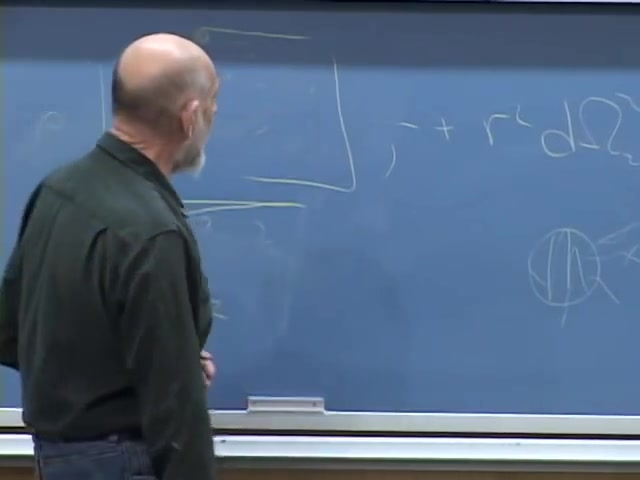
\includegraphics[width=0.76\textwidth]{lecture_09_figure_13.png}
\caption{黒板に書かれた、膨大な指数関数的待ち時間スケールを伴う再帰の議論。}
\lectureframe{01:16:24}
\end{figure}

そのような再帰の前には、より小さな揺らぎのほうがはるかに頻繁に起こる。部屋の中の分子がすべて一隅に集まることもあるかもしれない。複雑な渦が一時的に形成されることもあるかもしれない。講義の遊び心ある階層では、熱運動が象を組み立てることもあるかもしれない。要求されるエントロピー不足が小さいほど、その揺らぎはより安価である。

\begin{classroomqa}
\audiencequestion{ポアンカレ再帰は特に量子力学の帰結なのか。\lecturetimestamp{01:25:44}}
\lecturerresponse{いいえ。再帰と稀な揺らぎはすでに古典統計力学において生じる。それらをド・ジッター空間に適用する際には我々の現在の物理的枠組みを用いるが、それはいつか改訂されるかもしれない。しかし熱力学と統計的推論は、我々が知る最も頑健な構造の一つである。}
\end{classroomqa}

確率そのものの意味は、将来の理論においてより深まるかもしれない。サスキンドはそうでないとは主張していない。彼のより狭い論点は、統計力学の長期的な含意が奇妙であるというだけの理由でそれを放棄することは、物理学で最もよく検証された組織原理の一つを捨て去ることになる、というものである。

\section{ボルツマン脳と典型的観測者}

熱的な揺らぎがビッグバンのような状態全体を創り出すと仮定しよう。それには膨大なエントロピー減少が必要である。一つの太陽系を生み出す揺らぎはより安価であり、すでに暖かい地球はさらに安価である。唯一の要件が一人の観測者であるならば、最も費用のかからない揺らぎは、見かけの記憶を備えた機能する脳だけを創り出すかもしれない。そのような仮説的観測者はボルツマン脳と呼ばれる。

問題は、一つの奇妙な揺らぎが論理的に可能かどうかではない。ある宇宙論的モデルが、ほとんどすべての観測者はそのような揺らぎであると予測するかどうかである。我々は、自分たちが途方もなく非典型的であるとは仮定しないことによって、観測から推論する。首尾一貫した宇宙史を持つ通常の観測者が、孤立した熱的脳によって指数関数的に圧倒される理論は、その推論を損なう。

したがってボルツマン脳問題は、定量的な整合性のテストを名指ししている。通常の観測者の期待される存在量と、揺らぎから生まれた観測者の存在量を比較する。後者が支配するならば、それらが増殖する前に真空が崩壊しなければならないか、測度を変更しなければならないか、あるいは宇宙論的仮定を再検討しなければならない。

紫外--赤外の繋がりに関する以前の問いは、明示的に先送りされる。再帰の議論は、その別個の問題を解決することに依存していない。

\section{永遠のインフレーションと泡宇宙}

次に講義は、完全な導出を試みることなく、第二の確率問題を導入する。準安定なド・ジッター真空は、真空エネルギーがより低い泡を核生成しうる。泡の壁は膨張し、その内部は開いたフリードマン--ロバートソン--ウォーカー宇宙へと発展しうる。一方、周囲のインフレーション領域は膨張を続け、さらに多くの泡を核生成する。

\begin{figure}[htbp]
\centering
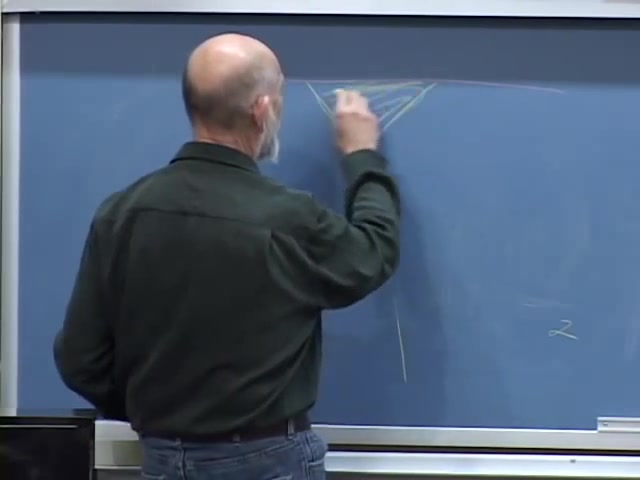
\includegraphics[width=0.74\textwidth]{lecture_09_figure_14.png}
\caption{膨張するド・ジッター背景の内部に描かれた、より低い真空エネルギーの泡。}
\lectureframe{01:29:38}
\end{figure}

決定的な特徴は指数関数的な個体数の増加である。新しい物理的体積は泡がそれを取り除くよりも速く生成されるため、泡領域の数は際限なく増大する。異なる泡は異なる低エネルギー状態に落ち着き、したがって異なる有効物理を示しうる。

統計的な困難を明らかにするため、サスキンドはまず宇宙論を離れ、有限だが未知の資源を持つ指数関数的に増加する人類人口を考える。観測者はこれまでに生きるすべての人々の中で典型的であると仮定する。人口が各世代で倍増し、その後終わるとすれば、全人類の半分は最後の世代に生き、四分の三は最後の二世代に生き、八分の七は最後の三世代に生きる：
\begin{equation}
f_n=1-2^{-n}.
\label{eq:l09-last-generations}
\end{equation}
その場合、典型性は、全資源供給について何も知らないにもかかわらず、われわれを不快なほど終末の近くに位置づける。これは人類絶滅の信頼できる予測として提示されているのではない。指数関数的成長が、数の集計をカットオフに支配させるという警告である。

コイン投げの例は、通常の典型性仮定をより明快に述べている。多数の実験者がそれぞれ公正なコインを\(N\)回投げるなら、圧倒的多数は
\begin{equation}
n_H=\frac{N}{2}+O(\sqrt{N}).
\end{equation}
を得る。極端な観測者は、証拠なしに自分が途方もなく稀な裾に位置すると仮定するよりも、まず悪いモデルか悪いコインを疑うべきである。宇宙論的確率も同じ典型性の直観を用いるが、無限の母集団においては、数を数えるための明確に定義された方法を必要とする。

\section{エッシャーの境界と測度問題}

サスキンドの幾何学的な類推は、M.\ C.\ エッシャーの\emph{円の極限 IV}、すなわち境界に向かって小さく見える天使と悪魔で敷き詰められた円盤である。その絵が表す双曲幾何学では、図形は等価であり、その見かけのユークリッド的な大きさは射影によってのみ変化する。

\begin{figure}[htbp]
\centering
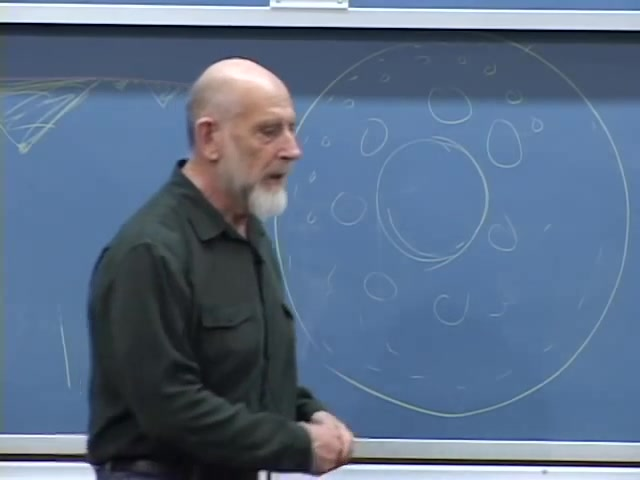
\includegraphics[width=0.76\textwidth]{lecture_09_figure_15.png}
\caption{円形の境界近くで指数関数的に増殖するエッシャーの図形に対応する黒板の代用図。}
\lectureframe{01:37:54}
\end{figure}

エッシャーが有限の時間、インク、忍耐しか持たないと想像しよう。縁の近くで彼はやがて描くのをやめ、おそらくいくつかの図形を未完成のまま残す。図形の数は双曲半径とともに指数関数的に増大するため、有限の外側の層は、描かれたすべての図形の一定の割合を含む。カットオフをどれほど外側へ動かしても、およそ半分が最終層に存在しうる。

次に天使と悪魔の比を問う。理想的な無限の模様では、対称性は一対一の等しさを示唆する。しかし任意の有限の数え上げでは、わずかに異なる境界が一方の型の図形をはるかに多く含みうる。数の大半は境界の近くにあるため、その境界の小さな変形が答えにオーダー1の変化を生む。

\begin{figure}[htbp]
\centering
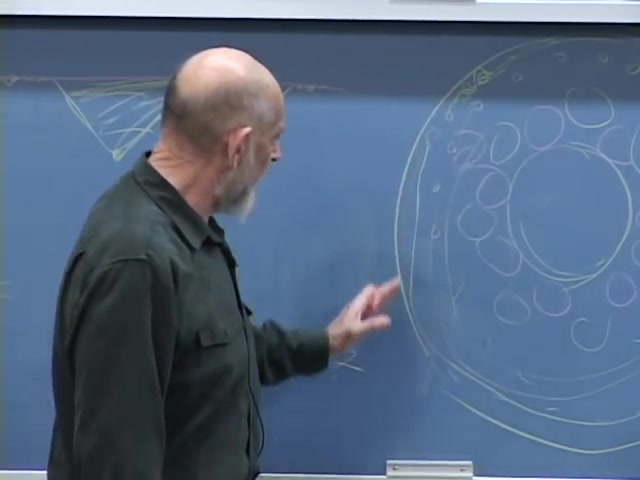
\includegraphics[width=0.76\textwidth]{lecture_09_figure_16.png}
\caption{指数関数的に増大する模様では、カットオフ境界が数の集計を支配する。}
\lectureframe{01:43:06}
\end{figure}

同じ曖昧さが永遠のインフレーションにも現れる。ある時間カットオフより下の青とピンクの泡宇宙を数え、次にカットオフをより後に押しやる。どちらの数も発散し、その比は\emph{時間}が何を意味するか、またカットオフ面がどのように描かれるかに敏感に依存しうる。確率測度とは、無限の母集団を正則化し、相対確率を抽出する処方である。異なるもっともらしい処方が一致しないことが測度問題である。

\begin{classroomqa}
\audiencequestion{このカットオフ問題と繰り込みの間に関係はありますか。\lecturetimestamp{01:45:43}}
\lecturerresponse{類推はある。量子場の理論では、格子または紫外カットオフを導入し、それを細かくし、正則化の縁の詳細に敏感でない量を求める。宇宙論者たちは永遠のインフレーションから同様に頑健な抽出を望んでいるが、ここで論じられる枠組みでは、それに匹敵する決定的な処方はまだ利用可能ではない。}
\end{classroomqa}

この類推を過大に評価すべきではない。繰り込みが成功するのは、制御された流れが正則化に依存しない観測量を特定する場合である。測度問題とはまさに、対応する不変な問いと極限手続きが不明瞭なままであるということである。われわれは間違った問いをしているのかもしれないと言うことは、正しい問いが提示されるまでは解決ではない。

\begin{classroomqa}
\audiencequestion{このバブル描像は、我々の初期宇宙におけるインフレーションと同じ現象なのか？\lecturetimestamp{01:48:19}}
\lecturerresponse{密接に関係している。永遠のインフレーションでは、親背景はインフレーションを続けながら、局所的なバブル内部は独自の宇宙論的進化を遂げる。我々の観測可能な宇宙は、そのような領域の一つの中に位置している可能性がある。}
\end{classroomqa}

\section{バブル衝突は観測できるか？}

二つのバブルは出会ったときに単に真空エネルギーを足し合わせるのではない。ドメインウォールが異なる真空状態を持つ領域を隔てており、その壁の幾何学がどちら側で何を観測できるかを決める。衝突の位置が我々の過去光円錐に対してどこにあるかに応じて、その痕跡は隠されることもあれば可視となることもある。

\begin{classroomqa}
\audiencequestion{二つの真空バブルが衝突すると何が起こるのか？\lecturetimestamp{01:52:07}}
\lecturerresponse{衝突はドメインウォールの幾何学を生み出し、その振る舞いは二つの真空と壁の張力に依存する。好都合な因果的条件の下では、その擾乱は我々の観測可能な領域に入り込み、異方的な痕跡を残しうる。}
\end{classroomqa}

この講義では、宇宙マイクロ波背景放射における低温領域を可能な候補として論じ、円形の特徴の周囲の偏光を判別要因として指摘する。これは意図的に、検出ではなく可能性として提示されている。説得力のある衝突の痕跡は革命的であろう。なぜなら、隣接するバブル領域の直接的な証拠を与え、測度問題を実験的に緊急のものとするからである。

\begin{figure}[htbp]
\centering
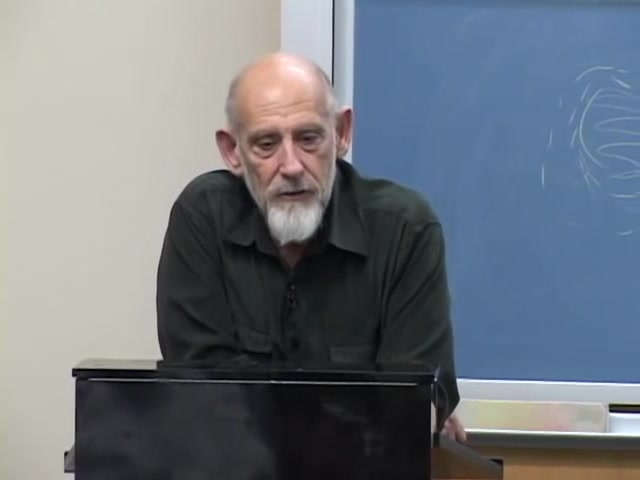
\includegraphics[width=0.70\textwidth]{lecture_09_figure_17.png}
\caption{バブル衝突の議論における円形の空の特徴とその可能な偏光パターン。}
\lectureframe{01:50:22}
\end{figure}

\editorialnote{低温スポットの議論は、講義当時の観測状況と提案を記録したものである。温度異常それ自体はバブル衝突の証拠ではなく、詳細で相関した痕跡が必要とされる。}

\begin{classroomqa}
\audiencequestion{バブルは四次元なのか、またその内部はどのような空間曲率を持つのか？\lecturetimestamp{01:53:37}}
\lecturerresponse{それらは時空領域であり、外部の時間の中で進化する三次元の石鹸膜ではない。その内部は典型的には負の空間曲率を持つ開いたFRW宇宙である。衝突はその幾何学を摂動するが、負の曲率を単純に正の曲率に変えるわけではない。}
\end{classroomqa}

\section{弦理論が確立することと確立しないこと}

最後の議論は、弦理論が正しい確率を割り当てるよう促すところから始まる。サスキンドは、その命題が曖昧すぎるとして数値を拒否する。代わりに彼は二つの主張を区別する。

第一に、量子力学と重力を組み合わせた高度に制約された数学的構造がある。それは精密な結果と深い数学的同一性を生み出し、その内部整合性は広範な精査に耐えてきた。講義の非公式な用語では、これは大文字の\(S\)を伴う\emph{String Theory}である。最も鋭く理解されている版は、超対称性に大きく依存している。

第二に、観測される世界は到達可能なエネルギーでは超対称ではない。厳密な超対称的構成を我々の非超対称的な宇宙に結びつけるには、超対称性の破れと、同じ精度では制御されないより大きな枠組みが必要である。講義の用語では、その望まれる拡張は小文字の\(s\)を伴う\emph{string theory}である。

\begin{classroomqa}
\audiencequestion{弦理論が自然の正しい理論である確率を割り当てることはできるか？\lecturetimestamp{01:54:18}}
\lecturerresponse{どの主張を意味するのかを特定せずに責任を持って行うことはできない。厳密な数学的構造は存在し、量子重力を含んでいるが、厳密に制御された超対称的模型は文字通り我々の観測する世界ではない。より大きな拡張が我々の世界を含むかどうかは、物理学者が情報に基づく先入観を持ちうる事柄であり、明確に定義された数値的確率ではない。}
\end{classroomqa}

完全な数学的機構が利用可能になる前の力学との類推である。\(F=ma\)と逆二乗の力を知っていても、高度に対称な円軌道しか解けないかもしれない。解ける部門は本物であろうが、理論全体ではない。同様に、厳密な超対称的弦構成は、より大きな構造の特別で異常に扱いやすい領域かもしれない。

\begin{figure}[htbp]
\centering
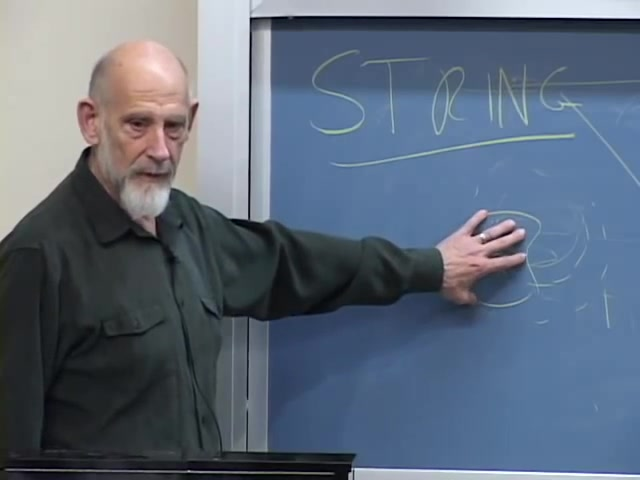
\includegraphics[width=0.60\textwidth]{lecture_09_figure_18.png}
\caption{講義の入れ子描像：推測的により大きな枠組みの中にある、厳密に制御された超対称的弦構成。}
\lectureframe{01:57:34}
\end{figure}

\begin{classroomqa}
\audiencequestion{なぜ厳密理論において単純に超対称性を破らないのか。\lecturetimestamp{01:57:02}}
\lecturerresponse{多くの近似的構成が超対称性の破れを研究しているが、完全に制御された非超対称的な骨格こそがまさに欠けているものである。標準的な近似を行った後に計算することはできるが、それらの近似が近づいていく厳密な対象を常に知っているわけではない。}
\end{classroomqa}

\begin{classroomqa}
\audiencequestion{厳密な超対称理論は、我々の世界を含むより大きな、より対称性の低い拡張を排除するのか。\lecturetimestamp{02:00:33}}
\lecturerresponse{否。それは観測される世界が厳密な超対称的セクターのみによって記述されないことを確立する。このセクターが現実的な物理を含むより大きな理論と結びついていることを証明も反証もしない。}
\end{classroomqa}

\begin{classroomqa}
\audiencequestion{弦の構成は、素粒子物理学の対称性の破れに類似した対称性の破れを含むのか。\lecturetimestamp{02:01:21}}
\lecturerresponse{超対称性の破れに関する広範な研究があり、超対称的な数学については多くが知られている。未解決の点は、現実的な破れを制御された近似のみならず完全な理論と組み合わせる、精密な非摂動的定式化である。}
\end{classroomqa}

\begin{classroomqa}
\audiencequestion{特殊相対性理論は弦理論において要請されるのか、それとも予言として現れるのか。\lecturetimestamp{02:03:02}}
\lecturerresponse{基礎となる規則はローレンツ不変である。たとえ物質で満たされた特定の背景が好ましい静止系を選び出しうるとしても。重力はさらに避けがたい。弦のスペクトルは、重力子の相互作用を持つ質量ゼロのスピン2の励起を含む。}
\end{classroomqa}

\begin{classroomqa}
\audiencequestion{弦理論は一般相対性理論および背景独立性と整合するのか。\lecturetimestamp{02:04:11}}
\lecturerresponse{その低エネルギー重力動力学は一般相対性理論と整合し、局所的な背景は動的に変化しうる。微妙な点は漸近的境界条件にある。それらは問題そのものを指定するものであり、一般にその時空内の局所的操作によって変えることはできない。}
\end{classroomqa}

講義は、堅牢な数学的核と未完成の物理的外挿との間のその区別で閉じられる。それは核が無用であるという判定でもなく、外挿が確立されたという主張でもない。厳密な知識がどこで終わるかを述べたものである。

\end{document}
